\documentclass[a4paper,12pt,twoside]{book}
\usepackage[a4paper,top=2.8cm,bottom=3.2cm,inner=3.2cm,outer=2.8cm,headheight=30pt]{geometry}

\UseRawInputEncoding

% Standard Latex math fonts and symbols packages
\usepackage{latexsym,amsfonts,amssymb,amsmath,amsthm,sansmath}

% Math packages
\usepackage{mathtools}

% Language package
\usepackage[english]{babel}
% \usepackage[latin1]{inputenc}
\usepackage{lipsum}

% Floats packages (put them in this way, otherwise images do not appear)
\usepackage{graphicx}
\usepackage{epstopdf}                   % allows the use of .eps graphics
% !TeX root = main.tex

\usepackage{tabularx}                   % tables package
\usepackage{multirow}
\usepackage{float} 					    % to place figures
\newcommand{\myfloatalign}{\centering}  % to center each float
\usepackage{caption}
\usepackage{subcaption}          
\usepackage[export]{adjustbox}          % to adjust figures box       
\captionsetup{format=hang,font=small}
%\usepackage{subfig}

%\usepackage{rotating} %to rotate figure and caption as well.

%\usepackage[TABTOPCAP,FIGBOTCAP]{subfig}  
\usepackage{fancyhdr}
\pagestyle{fancy}
\usepackage{colortbl}
\usepackage{color}
\usepackage{textcomp}	  % introduced to use \textquotesingle
%\usepackage{dropping}    % big letters

\usepackage{listings}   % code insertion
\usepackage{setspace}   % allow \singlespacing (by default) \onehalfspacing \doublespacing
\usepackage{longtable}
\usepackage{lscape}
\usepackage[T1]{fontenc}
% \usepackage{bookman}
\usepackage{booktabs}
\usepackage{array}
\usepackage[sort&compress,numbers]{natbib}


\usepackage{xr}                    % allow cross-referencing between different files

\usepackage{algorithm}		       % allow the inclusion of algorithms
\usepackage[noend]{algpseudocode}

\usepackage[titletoc]{appendix}    % to habe \begin{appendices} environment

\usepackage{pdfpages} % to insert a pdf into the latex document


%stuff for quotes

%% stuff for quotes ends


\usepackage{minted}


\usepackage{changepage}
%% stuff for definitions


%% stuff for definitions ends


% \usepackage[breaklinks=true, colorlinks,linkcolor=blue,citecolor=red]{hyperref}% PDF This must be the LAST package to allow a good performance!
\usepackage[bookmarks=true, breaklinks=true, colorlinks=true ,linkcolor=black, citecolor=black, urlcolor=black, linktocpage=true]{hyperref}% BW_PRINT  This must be the LAST package to allow a good performance!

\newcommand{\sans}[1]{\mbox{\sansmath$\mathsf{#1}$}} % command for sans mathematical font

% BState in algorithm package
\makeatletter
\def\BState{\State\hskip-\ALG@thistlm}
\makeatother

% Set vertical space between algorithm lines
\let\Algorithm\algorithm
\renewcommand\algorithm[1][]{\Algorithm[#1]\setstretch{1.3}}

% Define colors to be used un listings package
\definecolor{codegreen}{rgb}{0,0.6,0}
\definecolor{codegray}{rgb}{0.5,0.5,0.5}
\definecolor{codeblue}{rgb}{0.0,0.0,0.6}
\definecolor{backcolour}{rgb}{1.0,1.0,1.0}

% Define custom style for listings package
\lstdefinestyle{mystyle}{
    backgroundcolor=\color{backcolour},   
    commentstyle=\color{codegray},
    keywordstyle=\color{codeblue},
    numberstyle=\tiny\color{codegray},
    stringstyle=\color{codegreen},
    basicstyle=\tiny,
    breakatwhitespace=false,         
    breaklines=true,                 
    captionpos=b,                    
    keepspaces=true,                 
    numbers=left,                    
    numbersep=5pt,                  
    showspaces=false,                
    showstringspaces=false,
    showtabs=false,                  
    tabsize=2
}
 
\lstset{style=mystyle}

%
% %
% % i comandi seguenti impediscono la scrittura in maiuscolo
% % dei nomi dei capitoli e dei paragrafi nelle intestazioni
\renewcommand{\chaptermark}[1]{\markboth{#1}{}}
\renewcommand{\sectionmark}[1]{\markright{\thesection\ #1}}

%%Definisce lo stile del capitolo
\usepackage[Lenny]{fncychap}    %possibili anche Lenny,Sonny,Glenn,Conny
% \ChNameVar{\Huge\centering\bfseries}
% \ChTitleVar{\Huge\rm\bfseries}
\ChNameVar{\Huge\rm\centering}
\ChTitleVar{\Huge\rm\bfseries}
%%%%%%%%
% \newfont{\scaledfont}{cmr10 scaled 4000}

%----------------------LAYOUT---------------------------------
\fancypagestyle{plain} {
    \fancyhead{} \fancyfoot[C]{} \fancyfoot[LE,RO]{}
    \renewcommand{\headrulewidth}{0pt}
    \renewcommand{\footrulewidth}{0pt}
}

\fancypagestyle{main}{
	\fancyhead{}
    \fancyhead[LE,RO]{\rm\thepage}
    \fancyhead[LO]{\it\rightmark}
    \fancyhead[RE]{\it\leftmark}
    \fancyfoot{}
    \renewcommand{\headrulewidth}{0.4pt}
    \renewcommand{\footrulewidth}{0pt}
}

\pagestyle{main}
%\pagestyle{plain}

\addtolength{\textheight}{0.5cm}%2.2
\addtolength{\textwidth}{3cm} \addtolength{\voffset}{0.cm}
\addtolength{\headsep}{0.7cm}
\addtolength{\evensidemargin}{-1.35cm}
\addtolength{\oddsidemargin}{-1.35cm}
\renewcommand{\chaptermark}[1]{\markboth{#1}{}}
\renewcommand{\sectionmark}[1]{\markright{#1}{}}
\fancyhfoffset[H]{0.2cm} \setlength{\parindent}{0.1cm}
\setlength{\parskip}{0.05cm}
% \newenvironment{remark}[1][Remark]{\begin{trivlist}
% \item[\hskip \labelsep {\bfseries #1}]}{\end{trivlist}}

% % Environment to create theorems, Lemmas, Corollaries in italics with section numbering and Remark and Definition in roman style
\newtheorem{remark}{Remark}
\newtheorem{theorem}{Theorem}[section]
\newtheorem{corollary}[theorem]{Corollary}
\newtheorem{lemma}[theorem]{Lemma}

% \theoremstyle{remark}
% \newtheorem{remark}[theorem]{Remark}

\theoremstyle{definition}
\newtheorem{definition}[theorem]{Definition}


%tabular environment
\setlength{\heavyrulewidth }{0.1 em } %%top and bottom rule width
\setlength{\lightrulewidth }{0.03 em } %% mid rule width

%%CarosLAbra page layout
% %%%%%%%%%%%%%%%%%%%%%%%%%%%%%%%%%%%%%%%%%%%%%%%%%%%%%%%%%%%%
% % Page setup A4
% % On a4 (21cm width) we have 2.cm for the right margin
% % and 3.0 cm for the left margin giving 16.cm for the text.
% % Then we have
% % 3cm as margin on odd pages  ==> 3.0cm - 1in =  0.44cm
% % 2cm as margin on even pages ==> 2.0cm - 1in = -0.54cm
% %
% %%%%%%%%%%%%%%%%%%%%%%%%%%%%%%%%%%%%%%%%%%%%%%%%%%%%%%%%%%%%
% \oddsidemargin 0.44cm
% \evensidemargin -0.54cm
% %%%%%%%%%%%%%%%%%%%%%%%%%%%%%%%%%%%%%%%%%%%%%%%%%%%%%%%%%%%%
% % Page setup MAG
% % On a4 (21cm width) with mag 0.081 we leave
% % odd pages: 1 in. on the left and 16cm*0.81=12.96cm for the
% %            text giving 5.5cm for the right
% % Therefore for even pages:
% % 5.5cm-1in=2.96cm so setting 2.96cm/0.81=3.654cm as evenside
% % should work. The HP CLJ 3800 needs 4.148 to print correctly.
% %
% %%%%%%%%%%%%%%%%%%%%%%%%%%%%%%%%%%%%%%%%%%%%%%%%%%%%%%%%%%%%
% %\oddsidemargin 0.0cm
% %\evensidemargin 3.654cm
% %\evensidemargin 4.148cm
% %%%%%%%%%%%%%%%%%%%%%%%%%%%%%%%%%%%%%%%%%%%%%%%%%%%%%%%%%%%%
% \pretolerance=10000
% \tolerance=10000
% \topmargin -1.04cm
% \headheight 1.0cm
% \headsep 1.0cm
% \textheight 23.0cm
% \footskip 1.5cm
% \textwidth 16.0cm
% \parindent 0.7cm
% \textfloatsep 1.0cm
\renewcommand{\baselinestretch}{1.2}
% \newcommand{\stackunder}{\underset}
%
%
%
%
% %\numberwithin{equation}{section}  % Numera ecuaciones por secciones de capitulo
% \numberwithin{equation}{chapter}   % Numera ecuaciones por capitulo
% \setcounter{secnumdepth}{3}       % Profundidad para enumerar: 3 = \subsubsection
%
% \AtBeginDocument{
% \setlength{\abovedisplayshortskip}{-2pt}%
% \setlength{\belowdisplayshortskip}{13pt}%
% \setlength{\abovedisplayskip}{-2pt}%
% \setlength{\belowdisplayskip}{13pt}%
% }
%%CarlosLabra end

% %%spaziatura 1.5
% \onehalfspacing




\usepackage[T1]{fontenc}
\usepackage[utf8]{inputenc}

\usepackage{optidef}
\usepackage{amsmath}
\usepackage{amssymb}
\usepackage{amsthm}
\usepackage{bbm}
\usepackage{bm}
\newcommand{\norm}[1]{\left\lVert#1\right\rVert}
\usepackage{pdfpages}
\usepackage[titles]{tocloft}
% \setlength{\cftbeforetoctitleskip}{-10mm}

\begin{document}

% TITLE PAGE
\thispagestyle{empty}

{
\centering
\Large

~\vspace{\fill}

%\vspace{1cm}

{\Huge 
Reduced order models and machine learning techniques for digital twin applications
}

\vspace{2cm}

{\LARGE
Sebastian Ares de Parga Regalado
}

\vspace{3cm}
{\Large
Ph.D. thesis in Civil Engineering\\
Thesis submitted as a compendium of publications
\\[1em]
}

\begin{figure}[h]
	\centering
	
\includegraphics[width=4cm]{Figures/logo_camins}
\end{figure}


{\large
Universitat Polit\`ecnica de Catalunya\\
Barcelona School of Civil Engineering
}

\vspace{2cm}

\begin{tabular}{l l}
Supervisors: & Prof. Riccardo Rossi Bernecoli\\
             & Prof. Joaqu{\'i}n Alberto Hern{\'a}ndez Ortega
\end{tabular}

\vspace{\fill}

Barcelona, September 26, 2025

}


% ABSTRACT
\chapter*{Abstract}
\addcontentsline{toc}{chapter}{Abstract}

\noindent
This thesis advances intrusive projection-based reduced order modeling (PROM) as a scalable, physics-consistent foundation for real-time digital twins in industrial applications. By integrating high-fidelity numerical methods with robust model reduction techniques, it addresses the computational bottlenecks limiting the deployment of large-scale simulations for design, optimization, and operational monitoring.

Structured as a compendium of peer-reviewed articles, the work presents three key methodological contributions. First, it introduces a novel hyper-reduction framework for Petrov–Galerkin PROMs that eliminates the need for complementary meshes, enabling element-wise sampling fully compatible with standard finite element workflows, such as Kratos Multiphysics. Second, it proposes a scalable, HPC-enabled workflow for PROM training and deployment, leveraging parallel snapshot generation, distributed singular value decomposition, and a parallel version of the empirical cubature method, demonstrated on an industrial thermal digital twin of an electric motor. Third, it extends PROM methodologies into nonlinear regimes using latent-space closure strategies, including PROM-ANN and interpretable kernel-based surrogates (PROM-GPR, PROM-RBF), to overcome the Kolmogorov $n$-width barrier in convection-dominated flows. This extension includes a discrete physics-informed training strategy aligning neural network-based manifolds with the residual behavior of the underlying numerical scheme, ensuring physical consistency.

The developed methods are systematically validated on canonical model problems such as the inviscid one-dimensional Burgers' equation, and extended to industrial configurations like the Ahmed body wake flow using the AERO-F framework. Classical techniques, including piecewise-linear and quadratic manifolds, are also discussed to contextualize the limitations of global linear subspaces and motivate the nonlinear strategies presented.

All contributions have been implemented in the Kratos Multiphysics and AERO-F open-source frameworks, highlighting their practical applicability for large-scale engineering workflows. While this thesis does not implement a closed-loop digital twin, it provides a robust foundation for future \textit{Component Twins} and \textit{Asset Twins}, bridging high-fidelity modeling and real-time predictive capabilities.

Lastly, this thesis supports technology transfer through the \textit{SimTwins} spin-off initiative, delivering scalable and open-source digital shadows and digital twins tailored to meet emerging Industry 4.0 and 5.0 demands. Collectively, these contributions position intrusive projection-based ROMs as robust, interpretable, and high-performance tools essential for next-generation digital twin ecosystems.

\chapter*{Resumen}
\addcontentsline{toc}{chapter}{Resumen}

\noindent
Esta tesis desarrolla los modelos de orden reducido intrusivos basados en proyección (PROM) como base escalable y con consistencia física para habilitar gemelos digitales industriales con operación en tiempo real. Al integrar métodos numéricos de alta fidelidad con técnicas sólidas de reducción de modelos, aborda los cuellos de botella computacionales que dificultan el despliegue de simulaciones a gran escala para diseño, optimización y monitorización de la operación.

Estructurada como un compendio de artículos revisados por pares, la tesis presenta tres contribuciones metodológicas principales. En primer lugar, se propone un marco de hiperreducción para PROM de Petrov-Galerkin que elimina la necesidad de mallas complementarias y permite un muestreo a nivel de elemento plenamente compatible con los flujos de trabajo estándar de elementos finitos (por ejemplo, Kratos Multiphysics). En segundo lugar, se plantea un flujo de trabajo escalable habilitado para computación de alto rendimiento (HPC) para el entrenamiento y el despliegue de PROM, que aprovecha la generación paralela de instantáneas (snapshots), la descomposición en valores singulares (SVD) distribuida y una versión paralela del método de cubatura empírica (ECM), demostrada en un gemelo digital térmico industrial de un motor eléctrico. En tercer lugar, se extienden las metodologías PROM a regímenes no lineales mediante estrategias de cierre en espacio latente, incluidas PROM-ANN (redes neuronales artificiales) y modelos sustitutos interpretables basados en kernel, como PROM-GPR (regresión por procesos gaussianos) y PROM-RBF (funciones de base radial), con el fin de superar la barrera de la anchura n de Kolmogórov en flujos dominados por la convección. Esta extensión incorpora una estrategia de entrenamiento informada por la física discreta que alinea las variedades aprendidas con redes neuronales con el comportamiento del residuo del esquema numérico subyacente y garantiza la consistencia física.

Los métodos desarrollados se validan de forma sistemática en problemas canónicos, como la ecuación de Burgers unidimensional inviscida, y se trasladan a configuraciones industriales como la estela del cuerpo de Ahmed mediante el entorno AERO-F. Asimismo, se revisan técnicas clásicas, como las variedades lineales a trozos y las cuadráticas, para contextualizar las limitaciones de los subespacios lineales globales y motivar las estrategias no lineales propuestas.

Todas las contribuciones se han implementado en los marcos de código abierto Kratos Multiphysics y AERO-F, lo que subraya su aplicabilidad práctica en flujos de trabajo de ingeniería a gran escala. Aunque esta tesis no implementa un gemelo digital de bucle cerrado, proporciona una base sólida para futuros gemelos digitales de componente y de activo, y tiende un puente entre la modelización de alta fidelidad y las capacidades predictivas en tiempo real.

Por último, la tesis impulsa la transferencia tecnológica mediante la iniciativa SimTwins, que ofrece sombras digitales y gemelos digitales escalables y de código abierto, adaptados a las demandas emergentes de la Industria 4.0 y 5.0. En conjunto, estas contribuciones sitúan a los PROM intrusivos basados en proyección como herramientas robustas, interpretables y de alto rendimiento, esenciales para los ecosistemas de gemelos digitales de próxima generación.



% ACKNOWLEDGEMENTS
\chapter*{Acknowledgements}
\addcontentsline{toc}{chapter}{Acknowledgements}

\noindent
Quiero dedicar esta tesis especialmente a mi \textbf{familia}, por su amor incondicional y su apoyo en cada circunstancia. A mi esposa \textbf{Simonetta}, por todo tu amor y apoyo, porque sé que incluso en los momentos más difíciles siempre estuviste ahí para levantarme; porque este no es un esfuerzo individual y eres el mejor equipo. Gracias por acompañarme en cada aventura sin pensarlo y por ser siempre mi fuente de energía.

A mi mamá \textbf{María de los Ángeles}, por estar siempre pendiente de mi bienestar y por su apoyo constante en cada paso. A mi papá \textbf{Gonzalo}, por tus consejos y respaldo en los momentos clave, y por enseñarme con tu ejemplo a mantenerme firme ante los retos. A ambos, por su apoyo desde mis primeros estudios hasta ahora y por todo su amor que siempre me ha acompañado. A mis hermanos \textbf{Ángela} y \textbf{Gonzalo}, por estar ahí para conversar, escucharme y darme su apoyo sin condiciones. Y a \textbf{Fifa} y \textbf{Gol}, por darme tantas alegrías y recordarme disfrutar cada día. Una mención especial a mi grupo más cercano de amigos: \textbf{Jose}, \textbf{Juliana}, \textbf{Ricardo}, \textbf{Daniela} y \textbf{Laura}, por su amistad, risas y apoyo durante todos estos años.

\vspace{0.5cm}

I want to express my sincere gratitude to my \textbf{supervisors} \textbf{Riccardo Rossi} and \textbf{Joaquín Hernández} for being exceptional advisors, guiding me in my training as a researcher, and always supporting me in reaching my goals. Thank you for helping me grow both professionally and personally.

I am especially thankful to my \textbf{closest friend and collaborator} \textbf{Raul Bravo}, who worked side by side with me during my PhD thesis. It was truly an honor to work together, you made this journey smoother, more enriching, and full of valuable lessons.

I am also grateful to my \textbf{internal collaborators} at \textbf{CIMNE}: \textbf{Carlos Roig}, \textbf{Ruben Zorrilla}, \textbf{Nicolas Sibuet}, and \textbf{Marco Lopez}, for all the academic contributions, teamwork, and constant support throughout this thesis. Working with you was a pleasure. I also want to thank all the amazing people at \textbf{CIMNE} with whom I shared so many good moments during lunch breaks, coffee chats, and different activities: \textbf{Nicolò}, \textbf{Mehdi}, \textbf{Gabriel}, \textbf{Uxue}, \textbf{Andrea Gorgi}, \textbf{Shardool}, \textbf{Mirna}, \textbf{Rodi}, \textbf{Michele}, \textbf{Andrea Montanino}, \textbf{Agustina}, \textbf{Runeal}, \textbf{Ignacio}, \textbf{Carlos}, \textbf{Lu}, \textbf{Junior}, \textbf{Ricardo Tosi}, \textbf{Eduard}, \textbf{Pau}, \textbf{Saman}, \textbf{Polytimi}, \textbf{Henning}, \textbf{Mariano}, \textbf{Ivan}, \textbf{Javad}, and everyone who made the daily work so much better.

I would also like to thank my \textbf{broader collaborators}: \textbf{Stefan Boschert}, \textbf{Rosa M. Badia}, \textbf{Jorge Ejarque}, \textbf{Enrique Quintana}, \textbf{Andrés Tomás}, \textbf{Cristian Catalin}, \textbf{Jorge Vazquez}, \textbf{Karim}, \textbf{Giovanni Stabile}, and all the other members of the \textbf{eFlows4HPC project}, for our work together. These collaborations showed me the value of cross-institutional and cross-industry collaboration, broadened my perspective beyond academia, and strengthened my drive for research that has real impact across domains.

I am deeply grateful to \textbf{Professor Charbel Farhat} for inviting me as part of the \textbf{Fulbright program} and giving me all the tools for a fruitful collaboration. I am also thankful for my direct work with \textbf{Radek Tezaur} and \textbf{Carlos Hernández}, which made this experience even more rewarding. I also thank the whole \textbf{Stanford FRG team}: \textbf{Rodrigo}, \textbf{Jeremy}, \textbf{Faisal}, \textbf{Bruce}, \textbf{Brahmini}, \textbf{Taggart}, \textbf{Christian}, \textbf{Ali}, and the rest of the team, for the enriching discussions during my visit and for welcoming me as one more member of the group.

I truly appreciate the help and support of the \textbf{administrative staff} who guided me along the way: \textbf{Jordi Jiménez}, \textbf{Jazmin Rios}, \textbf{Silvia Aranda}, \textbf{Maria Roses}, \textbf{David Luna}, as well as \textbf{Carinna}, \textbf{Linnea}, and \textbf{Victoria} from \textbf{Fulbright} for their constant dedication and assistance.

I gratefully acknowledge the financial support of the \textbf{FI-SDUR program} (Department of Research and Universities, \textbf{Generalitat de Catalunya}), which funded the majority of my PhD research, including international stays, conferences, and summer schools. I also thank the \textbf{Universitat Politècnica de Catalunya (UPC)} and \textbf{CIMNE} for their institutional and financial support throughout my doctoral studies, including access to research infrastructure and funding for scientific dissemination. In this context, I extend my appreciation to the \textbf{Kratos Multiphysics Group} for their continuous collaboration and for supporting part of my research efforts. I am also thankful to the \textbf{eFlows4HPC European project} for providing access to tools and resources, and for supporting several dissemination and publication efforts related to this thesis. Additionally, I acknowledge the \textbf{X4HPC network} and \textbf{Barcelona Activa} for their support in my technology transfer and entrepreneurship training, through workshops, mentoring, and innovation programs. I further thank the \textbf{Stanford University Department of Aeronautics and Astronautics} for partially funding my research visit and providing a stimulating academic environment.  I am deeply grateful to the \textbf{Fulbright Program} for funding my Visiting Student Researcher stay at Stanford University, which marked a key stage in my academic and professional development.

\textit{This international research stay at Stanford University lasted eight months (October 2024 – June 2025) and meets the requirements for the International Mention of the PhD.}

Lastly, I want to thank all my \textbf{football teammates} from every team I have played with; you made every match unforgettable. And to my big \textbf{family in Mexico}, including all my lifelong friends from my hometown, thank you for always being there. The list would be way too long to include here, but you know who you are. And to everyone else who contributed in any way to this journey, thank you.



% TABLE OF CONTENTS
\tableofcontents
% \clearpage
% %% %%%%% List of Figures ******************************************
% \phantomsection
% \addcontentsline{toc}{chapter}{\protect\numberline{}List of Figures}
\listoffigures
\clearpage
 
\listoftables
\clearpage

% CHAPTER 1 - Introduction
\chapter{Introduction}

\section{Background and motivation}


Numerical simulations have become an indispensable tool across numerous domains of engineering and applied sciences, significantly impacting design, analysis, and optimization processes. Their use spans many areas: from the structural design of complex infrastructures \cite{carrera2014finite, ranzi2018structural}, advanced vehicle development \cite{stork2008towards}, to the modeling of intricate natural phenomena \cite{gingold1977smoothed}, and the optimization of industrial operations \cite{kiran2020numerical,davidson2003role}. By leveraging simulation-based approaches, researchers and engineers can explore, predict, and optimize the behavior of physical systems efficiently, significantly reducing dependence on costly, time-consuming, and potentially hazardous experimental campaigns \cite{belytschko2014nonlinear,zienkiewicz2005finite}.

The widespread adoption and success of simulation methods have been propelled by substantial advances in computational power, algorithmic accuracy, and the growing availability of high-resolution datasets \cite{Gunal2019Industry, Rodic2017Industry}. In recent years, these advancements have paved the way for transformative technological paradigms such as Industry 4.0 and, more recently, Industry 5.0. These paradigms integrate advanced simulations with real-time sensor data and artificial intelligence, fostering cyber-physical systems that exhibit greater autonomy, adaptability, and operational efficiency \cite{Agostino2020Using, Onggo2018SYMBIOTIC, Catelani2021From}. Within these evolving frameworks, high-fidelity simulations provide critical support for real-time decision-making, predictive analytics, and the design of intelligent manufacturing and monitoring systems \cite{Sandberg2019Current, Muhammet2021Industry, Muhuri2019Industry}.

Nevertheless, as model fidelity and complexity escalate, computational demands have grown considerably \cite{elmisaoui2023high}. High-resolution simulations, essential for accurately capturing intricate physical behaviors, often necessitate extensive computational resources and prolonged execution times on high-performance computing (HPC) infrastructures \cite{hosseini2016direct}. This computational intensity significantly limits their practical deployment in scenarios demanding rapid response, including real-time control \cite{ra2023real, ballin1988high}, extensive parametric optimization studies \cite{breitkopf2013multidisciplinary}, and continuous monitoring of dynamic systems \cite{dyskin2018computational}.

To overcome these limitations, the development and adoption of reduced order models (ROMs) have gained prominence. ROMs efficiently encapsulate the essential dynamics of complex systems within reduced-dimensional representations, achieving substantial reductions in computational cost while preserving the accuracy of the underlying high-fidelity models \cite{quarteroni2015reduced}. Integrating these ROMs with modern machine learning approaches has further enhanced their ability to effectively capture nonlinear behaviors, improve model generalization, and broaden applicability across varying operational conditions \cite{lee2020model}.

Furthermore, embedding ROMs within comprehensive operational frameworks, particularly digital twins, has opened new horizons for real-time simulation-based optimization and continuous system monitoring \cite{kapteyn2022data}. Digital twins, empowered by ROMs and machine learning, enable precise, dynamic, and actionable insights into physical systems, representing a powerful synthesis of simulation, data-driven modeling, and real-time analytics.

In this context, the research presented herein aims to advance the development and integration of ROM methodologies and machine learning techniques. The goal is to effectively address contemporary computational challenges, fostering more responsive, accurate, and cost-effective simulation solutions tailored to the rigorous demands of modern engineering and industrial applications.

Several European research initiatives provide a direct backdrop to these objectives. For instance, the \href{https://cordis.europa.eu/project/id/800898}{ExaQUte} project~\cite{tosi2021parallel} laid the theoretical and computational groundwork for scalable exascale simulations, particularly in uncertainty quantification (UQ) and optimization under uncertainty. In parallel, the \href{https://cordis.europa.eu/project/id/946009}{EdgeTwins} project extended these exascale-driven insights into real-time digital twins running on constrained devices, demonstrating the viability of linear ROMs in edge deployments. Building on both, the \href{https://www.eflows4hpc.eu/}{eFlows4HPC} project~\cite{ejarque2022enabling} offers a unified workflow framework that integrates HPC, data analytics, and artificial intelligence for large-scale digital twin deployment (see Figure~\ref{fig:rom_workflow_eflows}). Within these efforts, ROMs serve as the linchpin for bridging high-fidelity physics with the fast, adaptive, and resource-efficient requirements of modern cyber-physical systems.

\begin{figure}[ht]
    \centering
    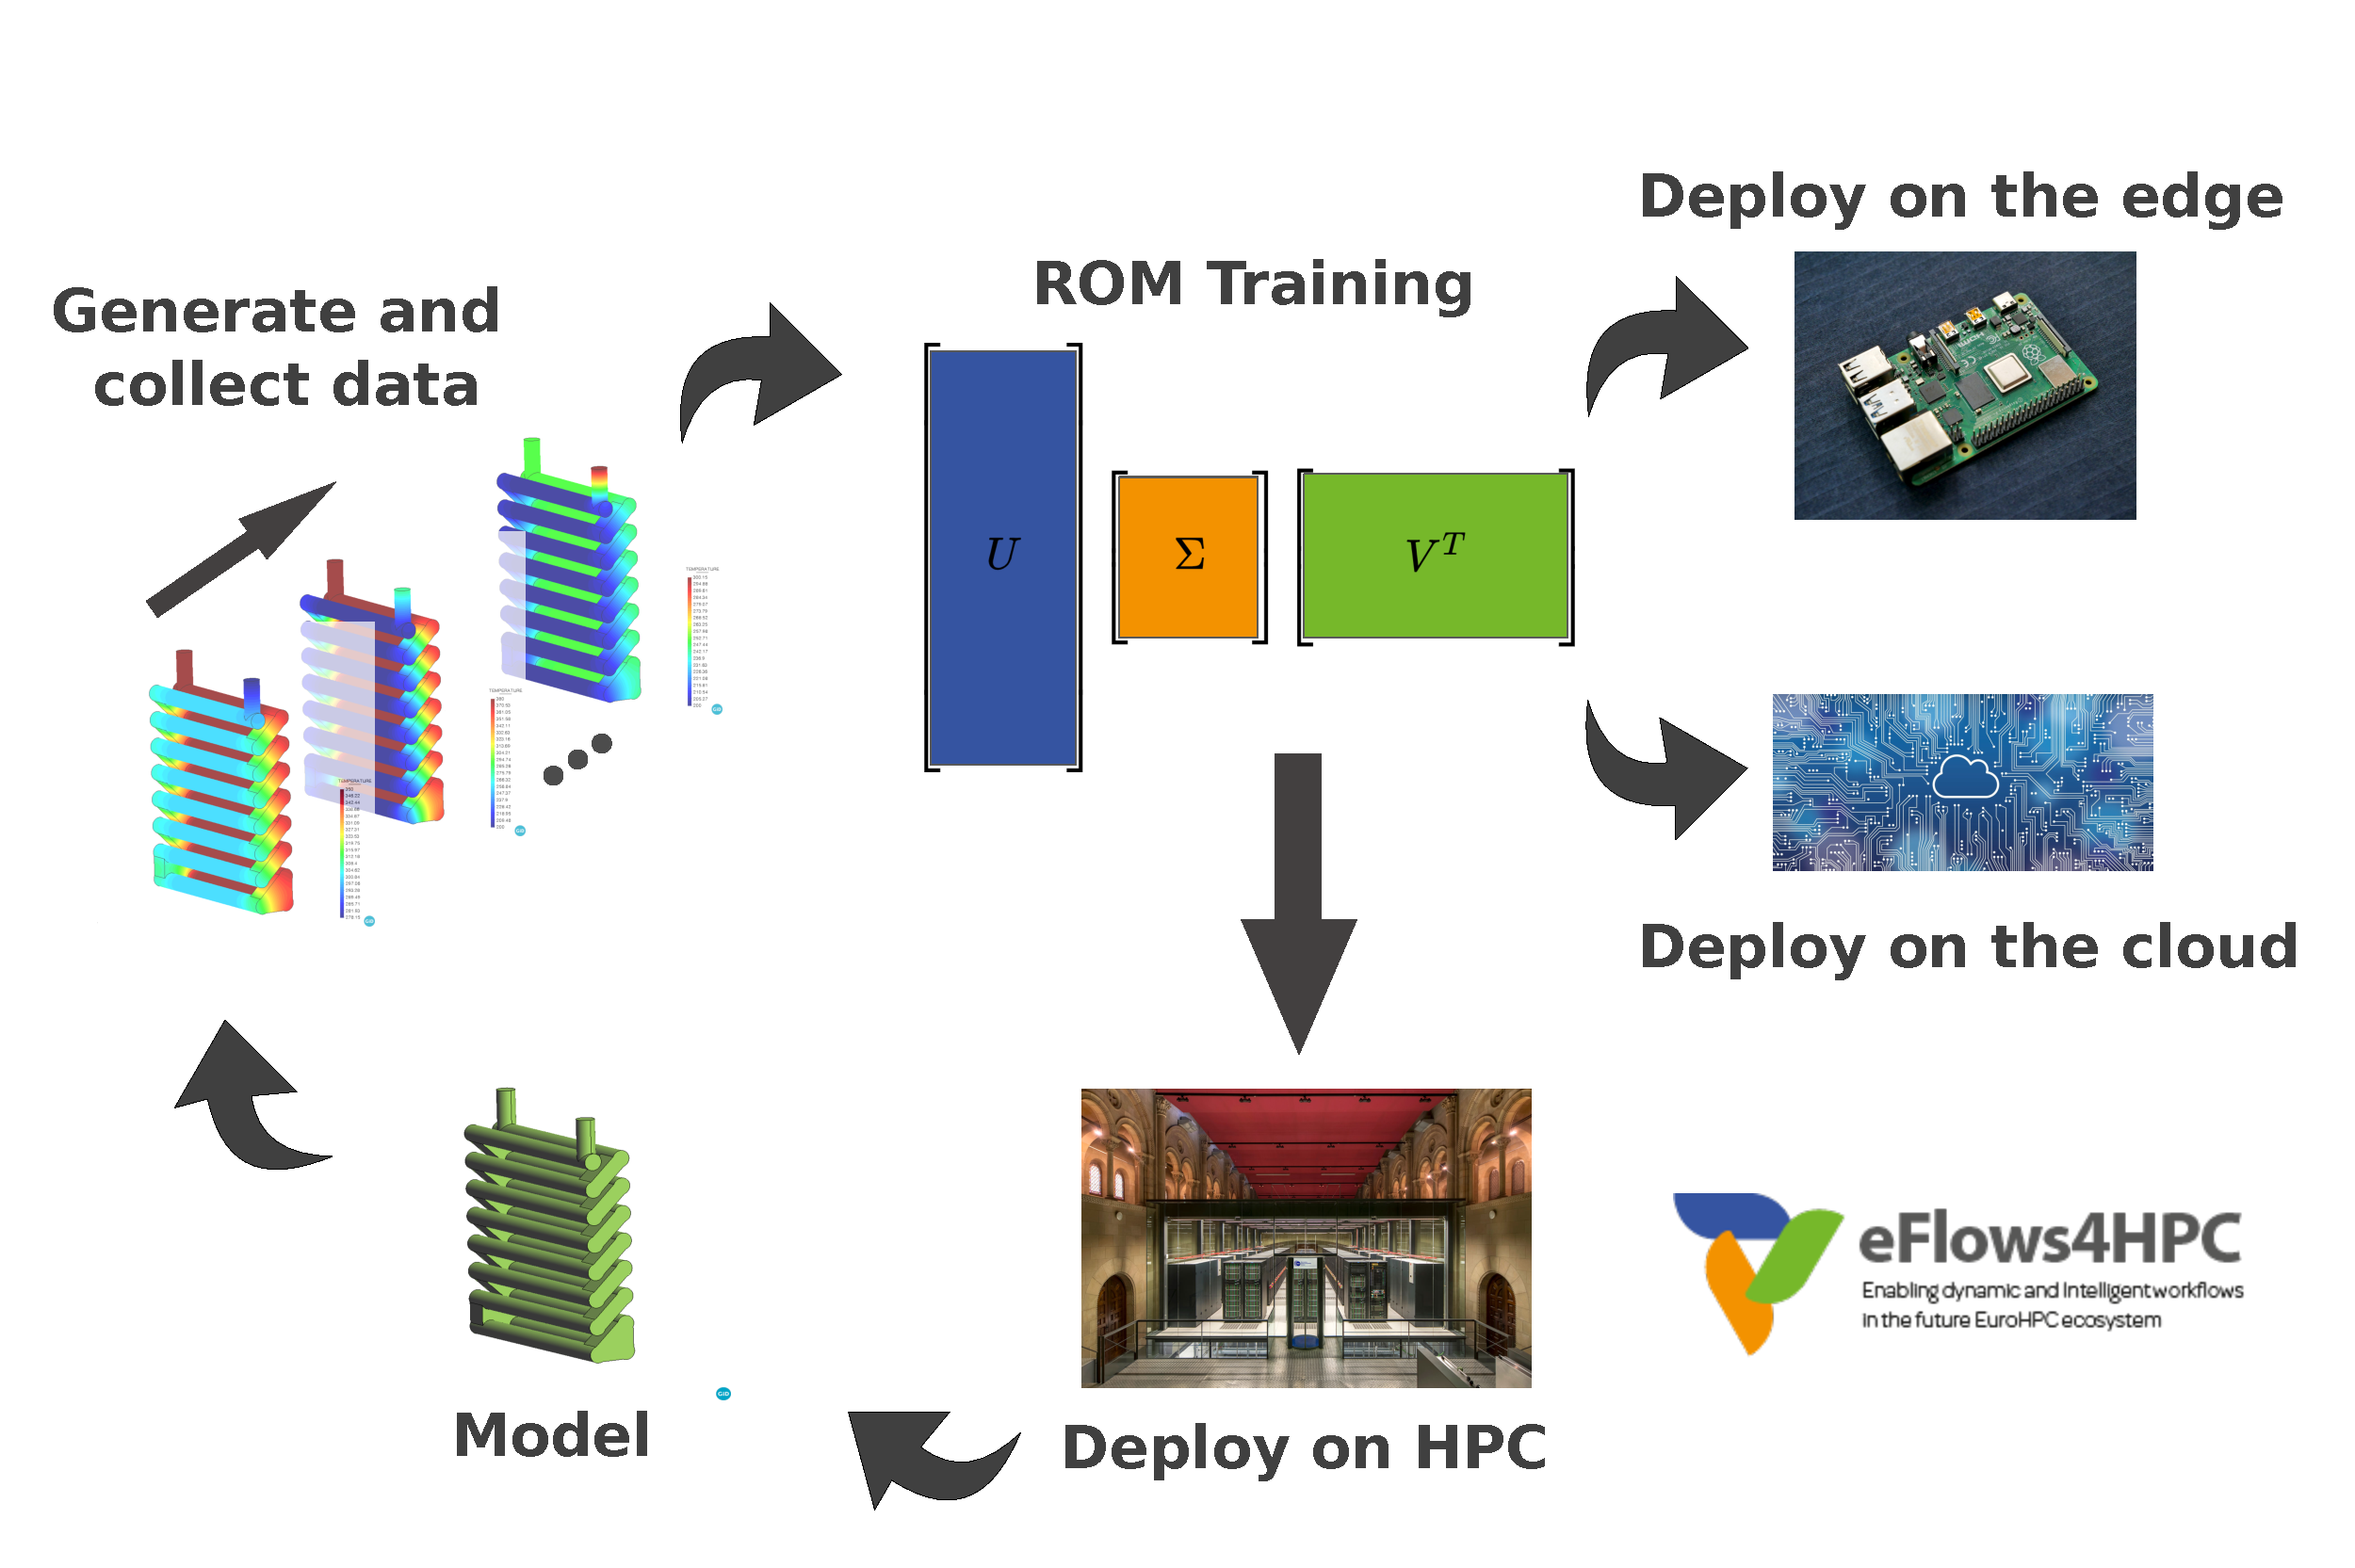
\includegraphics[width=0.92\textwidth]{Figures/Poster.pdf}
    \caption{Main phases in the ROM workflow: data generation using high-fidelity simulations, training via dimensionality reduction, and deployment on target platforms (cloud, edge, HPC). Adapted from~\cite{ejarque2022enabling}.}
    \label{fig:rom_workflow_eflows}
\end{figure}


By leveraging this broader ecosystem of HPC-enabled simulation, reduced order modeling, and digital twin technologies, the present thesis consolidates and extends these efforts through four core research directions:

(1) the development of hyper-reduction techniques for Petrov–Galerkin projection-based ROMs, enabling efficient acceleration for convection-dominated systems~\cite{Ares2023};

(2) the design of scalable, parallel workflows for the training and deployment of projection-based reduced order models on HPC infrastructures, enabling real-time digital twin applications~\cite{Ares2024};

(3) the introduction of a discrete physics-informed training strategy for projection-based ROMs, ensuring that learned nonlinear manifolds remain consistent with the governing residual structure during intrusive projection~\cite{sibuet2025discrete};

and (4) the extension and systematic assessment of nonlinear closure strategies based on machine learning, specifically, radial basis functions (RBF) and Gaussian processes (GP), to improve robustness and interpretability for strongly nonlinear problems~\cite{de2025nonlinear}.

Together, these contributions address key computational bottlenecks and advance the state-of-the-art and practical deployment of projection-based ROMs in high-dimensional, real-time industrial digital twin applications.



\section{Literature review}
\subsection{High-fidelity modeling: Numerical methods in engineering}

High-fidelity numerical simulations are essential tools for understanding, predicting, and optimizing complex physical phenomena in engineering. These simulations are generally based on mathematical models expressed as partial differential equations (PDEs), which describe diverse physical behaviors across numerous disciplines. Due to the inherent complexity of solving PDEs analytically, numerical methods have become indispensable for practical engineering solutions.

Among the most established and versatile numerical approaches are the Finite Element Method (FEM), particularly effective for structural mechanics, fluid-structure interaction, and multiphysics simulations \cite{zienkiewicz2005finite,onate2009structural}; the Finite Difference Method (FD), widely used for wave propagation, heat conduction, and electromagnetics due to its simplicity and ease of implementation \cite{mitchell1980finite,taflove2005computational}; and the Finite Volume Method (FV), favored for fluid dynamics applications owing to its robust enforcement of conservation principles across control volumes \cite{versteeg2007introduction,moukalled2016finite}. Throughout this thesis and its associated publications, these three methodologies constitute the core numerical strategies employed.

Each of these high-fidelity numerical methods has achieved remarkable maturity, integrating advanced discretization techniques, adaptive meshing, and multiphysics coupling. However, their high accuracy comes at significant computational costs, demanding extensive computational resources and specialized hardware, particularly problematic in real-time, optimization-driven, or resource-constrained scenarios. These limitations motivate the pursuit of faster, more efficient surrogate models that can emulate high-fidelity simulations at a fraction of the cost, particularly ROMs, which offer a promising trade-off between accuracy and computational efficiency. The ROMs developed and analyzed in this thesis are consistently formulated using a discrete residual framework, ensuring seamless integration across FEM, FD, and FV schemes. These models are implemented using a combination of open-source and in-house simulation tools, including 
\href{https://github.com/KratosMultiphysics/Kratos}{Kratos Multiphysics}~\cite{dadvand2010object}, 
\href{https://bitbucket.org/frg/aero-f/src/master/}{AERO-F}, 
and academic solvers developed in Python and C++.



\subsection{Reduced order modeling}

The high computational cost associated with high-fidelity numerical simulations has motivated the development of surrogate modeling strategies capable of accelerating repeated or real-time evaluations. In many applications, including parametric studies, optimization loops, uncertainty quantification, and digital twins, traditional solvers become impractical due to their high dimensionality and intensive resource demands~\cite{brunton2022data, rozza2022advanced}.

ROMs offer a powerful alternative by seeking low-dimensional representations that approximate the behavior of complex systems with significantly reduced computational effort. The central assumption behind ROMs is that, despite the high dimensionality of the full-order model (FOM), the set of solutions of interest often lies on or near a low-dimensional manifold embedded in the high-dimensional space~\cite{ryckelynck2024manifold}.

Among the most widely used ROM techniques are those based on linear dimensionality reduction. The Proper Orthogonal Decomposition (POD) is one of the most established methods and extracts dominant modes from a set of solution snapshots (see Figure~\ref{fig:pod_snapshots_overview}) using techniques such as singular value decomposition (SVD), which provides a compressed, low-rank approximation of the snapshot matrix by extracting a reduced basis from its dominant patterns (see Figure~\ref{fig:svd_illustration})~\cite{Sirovich1987, Balachandar1998}.
Other classical approaches include the Reduced Basis (RB) method~\cite{hesthaven2016certified, hesthaven2022reduced}, which constructs reduced spaces tailored to parametric PDEs, and the Proper Generalized Decomposition (PGD)~\cite{nouy2010priori}, which decomposes multivariate functions into separable representations.

\begin{figure}[htbp!]
    \centering
    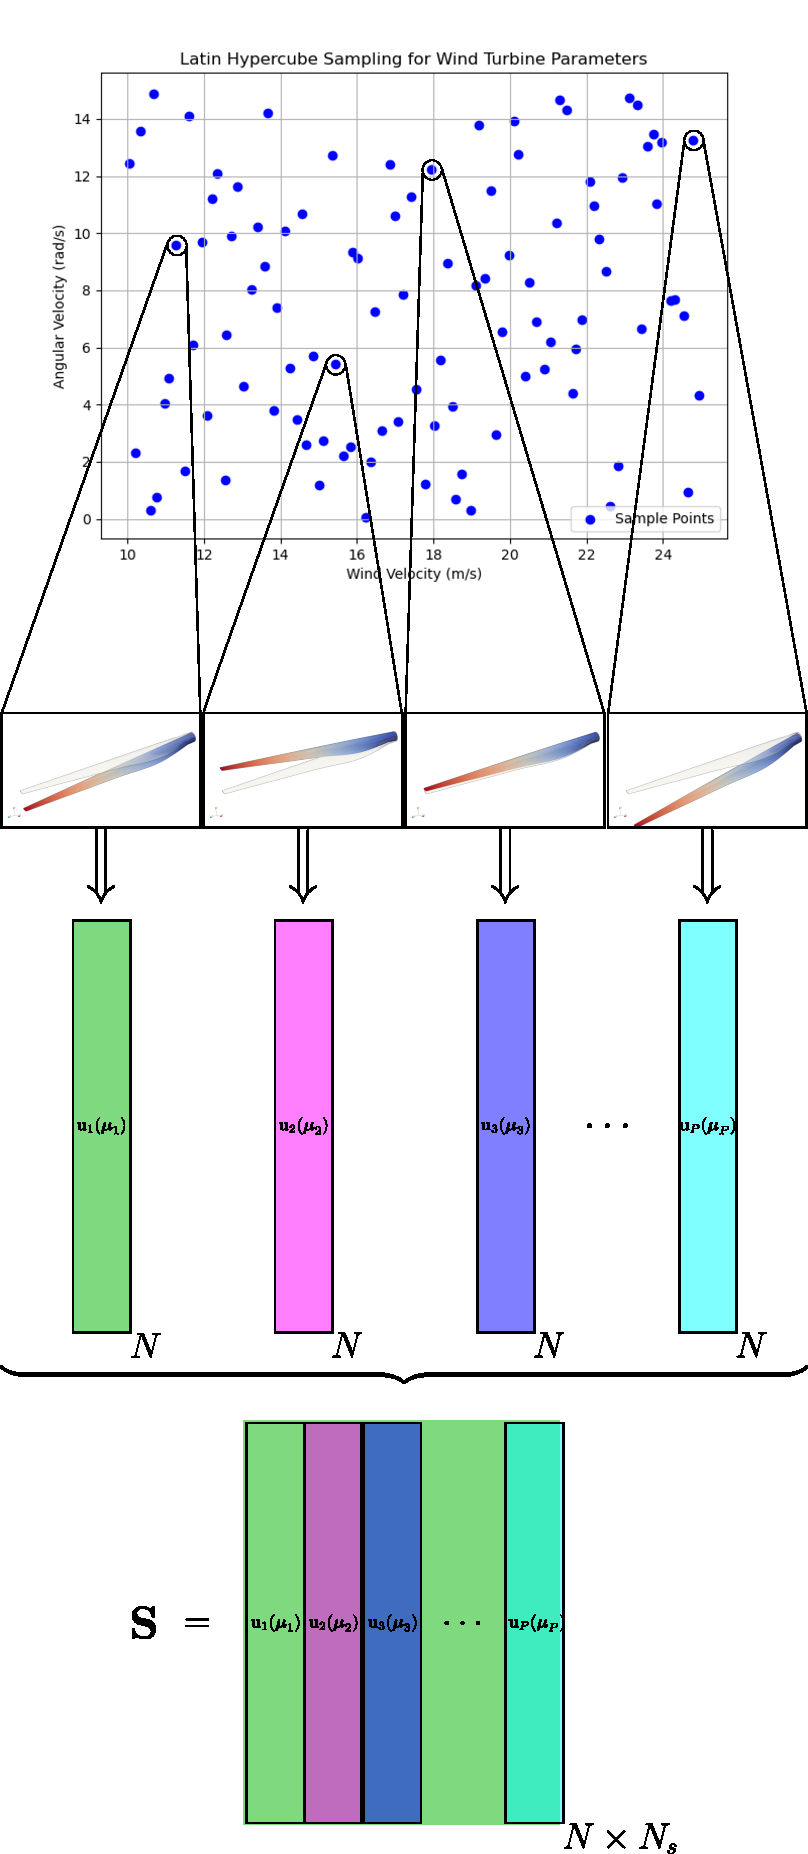
\includegraphics[width=0.5\textwidth]{Figures/SnapshotMatrixConstruction.pdf}
    \caption{Illustration of snapshot matrix construction for a structural model of a wind turbine blade. A set of training points, here defined by angular velocity and wind speed (sampled via Latin Hypercube Sampling), leads to parallel high-fidelity simulations whose results are stored in vectors and stacked to form the snapshot matrix~$\mathbf{S}$.}
    \label{fig:pod_snapshots_overview}
\end{figure}

\begin{figure}[htbp!]
    \centering
    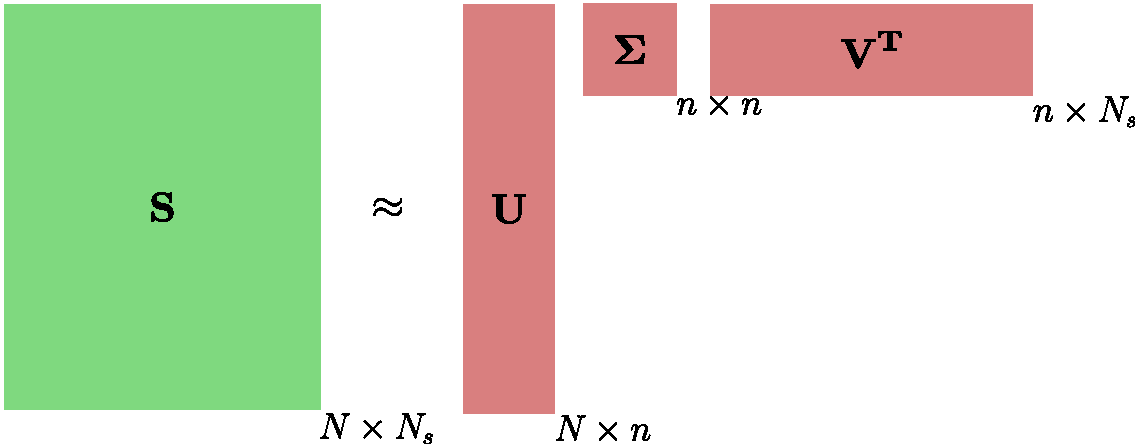
\includegraphics[width=0.7\textwidth]{Figures/SVD_Decomposition.pdf}
    \caption{Visual interpretation of the Singular Value Decomposition. The high-dimensional snapshot matrix~$\mathbf{S}$ is approximately factorized into a reduced basis~$\mathbf{U}$, a diagonal matrix of singular values~$\boldsymbol{\Sigma}$, and temporal or parametric coefficients~$\mathbf{V^T}$. This structure allows for compression and efficient low-dimensional representation.}
    \label{fig:svd_illustration}
\end{figure}



A robust strategy for constructing ROMs, known as projection-based reduced order models (PROMs), involves projecting the governing equations of the full-order model onto a reduced space spanned by the dominant modes (see Figure~\ref{fig:galerkin_prom_visual}). These PROMs rely on the assumption that the system dynamics can be accurately represented in a lower-dimensional subspace derived from high-fidelity snapshots. In the classical Galerkin projection, the residual of the governing equations is enforced to be orthogonal to the reduced basis, making it particularly effective for problems with symmetric positive definite (SPD) operators~\cite{carlberg2017galerkin, benner2015survey, Rowley2004}. For more general problems, especially those dominated by convection or exhibiting non-symmetric Jacobians, the Least-Squares Petrov–Galerkin (LSPG) approach offers a more robust alternative by minimizing the discrete residual in a least-squares sense~\cite{carlberg2011efficient}. While LSPG has proven effective in finite difference and finite volume contexts, its implementation in finite element settings often requires auxiliary constructions to enable efficient approximation. In this thesis, we explore an alternative yet equivalent Petrov–Galerkin formulation tailored for finite element discretizations, specifically designed to preserve element-level assembly during least-squares residual minimization. This modification anticipates the challenges posed by hyper-reduction in nonlinear settings and enables seamless integration of PROMs with efficient mesh-based approximation strategies~\cite{Ares2023}.

\begin{figure}[ht]
    \centering
    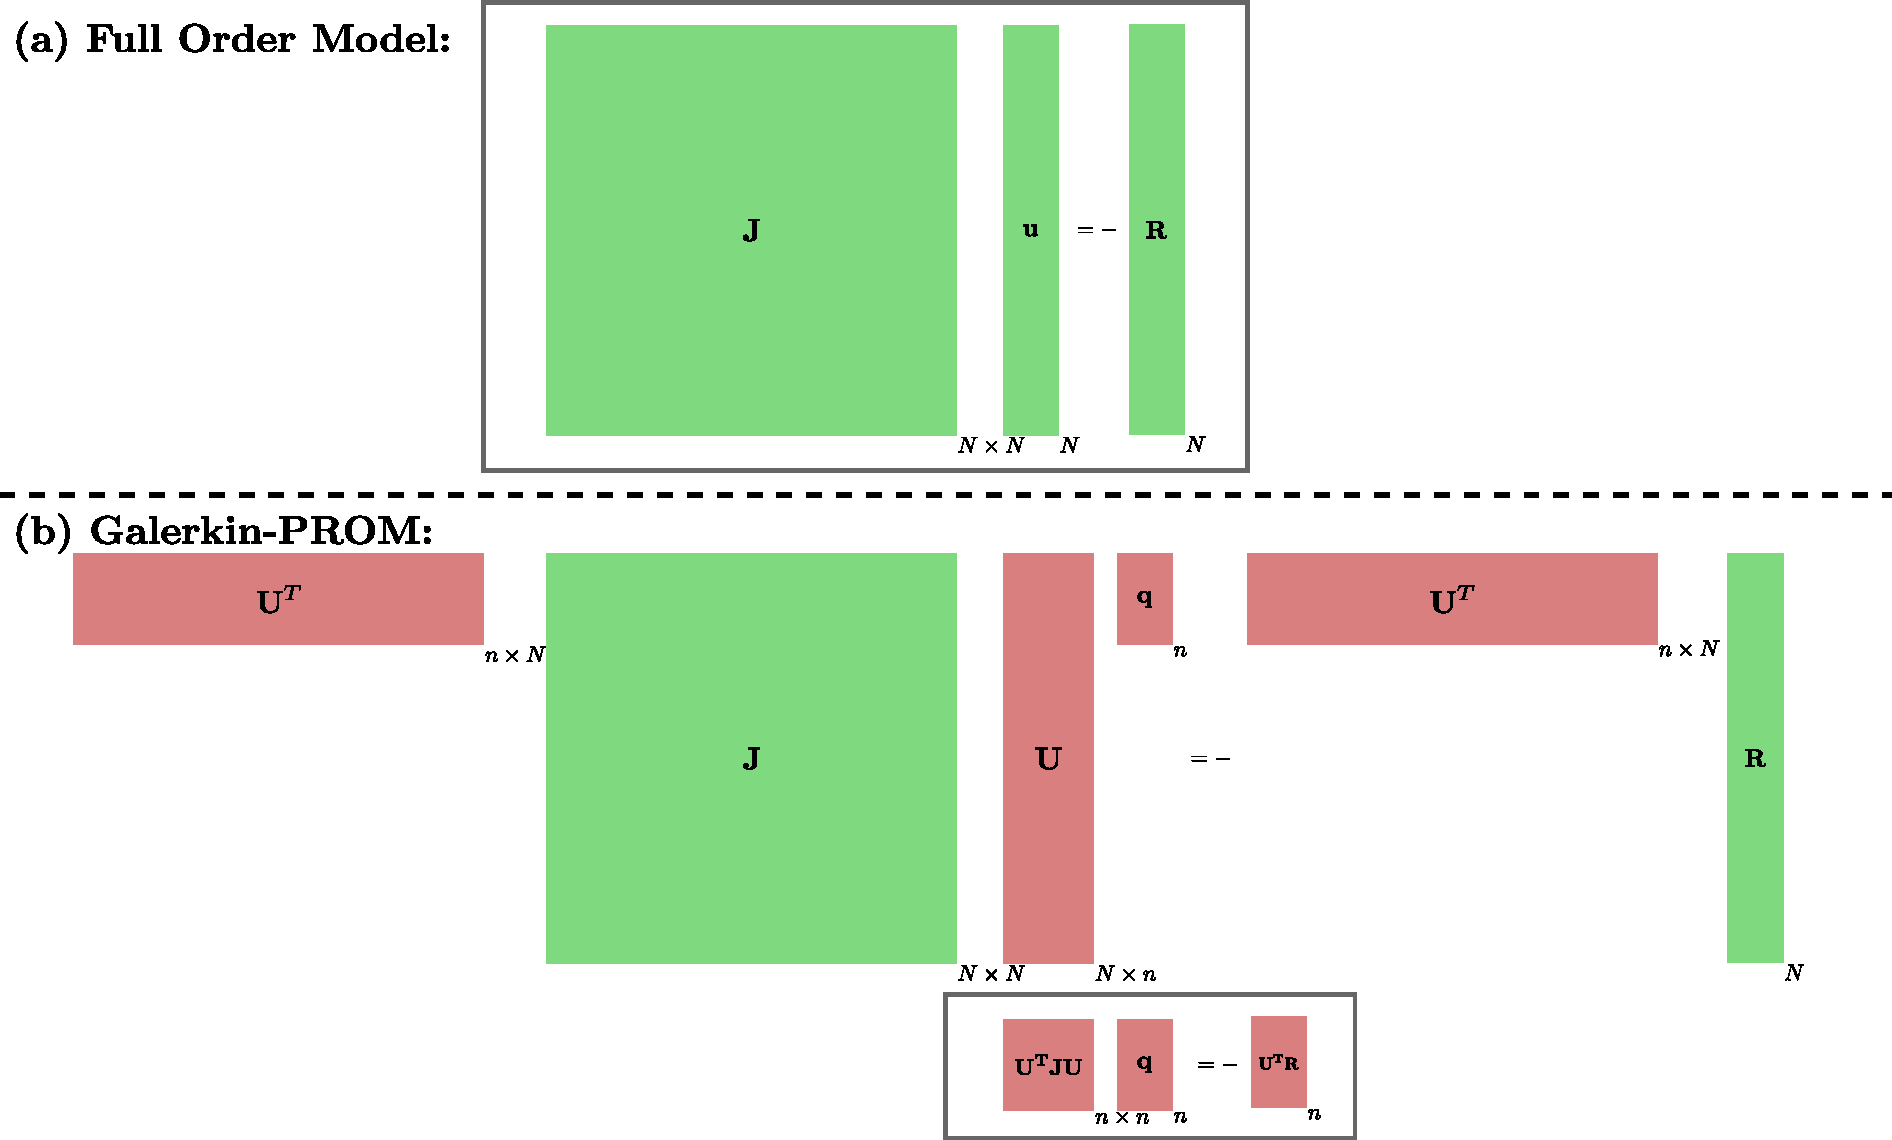
\includegraphics[width=0.95\textwidth]{Figures/SystemReduction.pdf}
    \caption{Schematic comparison between the full-order model and its Galerkin projection-based reduced order model. The full system of dimension~$N$ is projected onto a reduced space of dimension~$n$ using a basis~$\mathbf{U}$, yielding a smaller system with the same governing structure but much lower computational cost.}
    \label{fig:galerkin_prom_visual}
\end{figure}


Projection-based methods have been extensively applied in combination with different spatial discretizations, including finite elements, finite volumes, and finite differences~\cite{balajewicz2016projection,mcclellan2020projection,lucia2003projection}. These methods can be broadly categorized according to their level of intrusiveness. \textit{Intrusive ROMs} require direct access to the governing equations or their discretized form, as they project and assemble reduced systems explicitly. This is the category where the present thesis is primarily situated. In contrast, \textit{Non-intrusive ROMs} treat the original model as a black box and rely exclusively on input–output data pairs. Among the most common approaches are regression-based strategies like PODI~\cite{demo2019non}, POD-RBF~\cite{ostrowski2008solving}, POD-GP~\cite{ma2021data}, and POD-NN~\cite{hesthaven2018non}, which combine POD-based basis construction with surrogate models that map physical or parametric inputs to the generalized coordinates, using general interpolation strategies, radial basis functions, Gaussian processes, or neural networks, respectively.

Between these two ends lies a growing class of \textit{hybrid} or \textit{gray-box} approaches, which seek to blend physical modeling with data-driven flexibility. Notably, \textit{operator inference} methods~\cite{Peherstorfer2016,benner2020operator} and \textit{physics-informed neural networks} (PINNs)~\cite{raissi2019physics, chen2021physics} attempt to incorporate governing physics either as soft constraints or as part of the optimization process. Recent developments have extended these ideas to more structured formulations that combine PINNs with discrete numerical schemes such as the finite element method~\cite{gao2022physics,as2022mechanics}.

Despite their differences, all these techniques aim to reduce computational complexity without compromising the essential physical accuracy of the simulation. The methods studied in this thesis focus primarily on \textit{intrusive projection-based ROMs}, where access to the residual and its discrete structure enables greater control over accuracy and stability, as well as the ability to incorporate physics-consistent formulations and efficient approximation techniques.

Nonetheless, when dealing with nonlinear problems or parametrically rich systems, even the evaluation of reduced operators can become a computational bottleneck. In such cases, hyper-reduction methods are introduced to alleviate the cost of evaluating residuals and Jacobians, which would otherwise scale with the full-order dimension. Hyper-reduction techniques can be broadly categorized into two main philosophies: \textit{approximate-then-project} and \textit{project-then-approximate}. In the first category, nonlinear terms are approximated before projection using a reduced set of interpolation points. This includes the Empirical Interpolation Method (EIM)~\cite{barrault2004empirical}, its discrete variant, the Discrete Empirical Interpolation Method (DEIM)~\cite{chaturantabut2010nonlinear}, and the Gauss–Newton with Approximated Tensors (GNAT) method~\cite{Carlberg2013}, which integrates DEIM-like approximations within a least-squares Petrov–Galerkin framework. In the second category, the full-order residual is first projected and then approximated, preserving key structural and variational properties of the original problem. Prominent examples of this \textit{project-then-approximate} class include the Energy-Conserving Sampling and Weighting (ECSW) method~\cite{Farhat2015, grimberg2021mesh} and the Empirical Cubature Method (ECM)~\cite{hernandez2017dimensional, hernandez2020multiscale, Hernandez2024}, which construct efficient cubature rules for element-level assembly in reduced systems. As previously anticipated, this thesis extends the applicability of these techniques by introducing a Petrov–Galerkin projection strategy that preserves compatibility with element-wise hyper-reduction, even when minimizing the full discrete residual as in LSPG~\cite{Ares2023}.

Despite their efficiency, PROMs built on linear subspaces face fundamental limitations when dealing with systems characterized by complex nonlinear behavior. These models rely on the assumption that the solution manifold can be well-approximated by a low-dimensional linear subspace. However, in many practical scenarios, such as advection-dominated flows, moving discontinuities, or sharp fronts, the Kolmogorov $n$-width decays slowly, meaning that a large number of modes is required to capture the solution accurately~\cite{ohlberger2015reduced, peherstorfer2020model, ohlberger2013nonlinear, dahmen2014double, taddei2015reduced}. As a result, linear ROMs may become inefficient or lose predictive power in such regimes.

To overcome these limitations, a variety of nonlinear reduced order modeling strategies have been developed. \textit{Local ROMs}, also known as piecewise linear ROMs or Local POD, partition the parameter space into clusters and construct separate reduced bases for each region, improving expressiveness while maintaining linear structure locally~\cite{amsallem2012nonlinear, grimberg2021mesh}. Another approach involves enriching the reduced space with nonlinear terms, such as in \textit{quadratic ROMs}, which approximate the solution manifold using a quadratic expansion in the reduced coordinates, allowing for more accurate and compact representations of nonlinear dynamics~\cite{barnett2022quadratic}.

More recent advances leverage machine learning to construct nonlinear latent representations of the solution manifold. \textit{Autoencoder-based ROMs} (AE-ROMs), and particularly \textit{convolutional autoencoder ROMs} (CAE-ROMs), use neural networks to learn nonlinear encoders and decoders that map between high-fidelity fields and low-dimensional latent variables, enabling the capture of complex solution features with fewer reduced or generalized coordinates~\cite{lee2020model, romor2023non}. While these approaches have shown promise in high-dimensional settings, they often rely on structured mesh data and convolutional architectures, which limit their applicability to regular geometries. To overcome this, recent developments explore the use of graph neural networks (GNNs) to generalize autoencoder-based methods to unstructured meshes and irregular domains~\cite{gao2022physics}.

Nevertheless, these models are typically trained and evaluated over the full-order field, making them less suitable for large-scale problems with millions of degrees of freedom, such as those encountered in industrial applications. One could imagine overcoming this limitation by adapting the POD-DL-ROM strategy~\cite{FRESCA2022114181}, which performs an initial POD on the snapshot data before learning a further nonlinear compression, to an intrusive setting. However, in the current context of PROMs, a more scalable alternative is offered by \textit{neural-network-augmented projection-based ROMs}, where the core physics-embedded structure of the reduced model is preserved. In particular, PROM-ANN introduces a learned nonlinear correction term that approximates the closure error induced by projecting the governing equations onto a reduced basis~\cite{barnett2023neural, chmiel2025unified}. Crucially, the neural network operates entirely in the reduced latent space, mapping the primary generalized coordinates to secondary ones, and thus avoids any dependency on the high-dimensional FOM size~\footnote{This approach maintains compatibility with hyper-reduction techniques and should not be confused with non-intrusive regressors like POD-NN, as it remains embedded in a fully intrusive, projection-based framework.}.

To strengthen the physical consistency of such neural-network-based manifolds, this thesis further proposes a discrete physics-informed training strategy for PROMs, which augments standard latent-space training with a residual-based loss derived directly from the governing discretization. In parallel, to broaden the applicability of nonlinear PROMs to regimes with limited data availability or increased interpretability demands, this work also explores alternative closure strategies that replace the neural network in PROM-ANN with radial basis functions (RBF) and Gaussian processes (GP)~\cite{de2025nonlinear}. These approaches retain the desirable properties of PROM-ANN, such as scalability and compatibility with hyper-reduction, while offering more deterministic behavior and transparent functional forms, which can be advantageous in engineering design, control, and certification contexts.

Given their potential to deliver fast, accurate, and physically consistent approximations, ROMs, and in particular projection-based models, play a central role in enabling real-time capabilities and decision-making in modern simulation frameworks. However, the construction and deployment of PROMs for industrial-scale problems remain a challenge due to the cost of generating training data and computing reduced bases from massive high-dimensional datasets. To address this, the present thesis develops an HPC, parallel workflow for constructing PROMs, combining distributed snapshot generation, parallelized singular value decomposition algorithms, and partitioned hyper-reduction techniques. This scalable end-to-end infrastructure, designed for deployment via Functional Mock-up Units (FMUs), enables the transition of ROMs from research prototypes to real-time industrial digital twins~\cite{Ares2024}.


\subsection{Digital twins and their connection to ROMs}

Digital twins (DTs) are dynamic, simulation-enabled representations of physical assets that maintain real-time links with their counterparts through continuous data exchange, sensing, and modeling. Recognized as a top strategic technology trend~\cite{panetta2018gartner}, digital twins have evolved from simple CAD models into intelligent, integrated frameworks combining high-fidelity simulations, sensor analytics, and artificial intelligence. This fusion supports predictive analytics, diagnostics, prognostics, autonomous control, and informed decision-making within closed-loop cyber-physical architectures~\cite{boschert2016digital, rosen2019next, grieves2014digital}.

Modern digital twins are understood not merely as single models but as evolving ecosystems of digital artifacts interacting throughout the lifecycle of physical systems, from design to operation, maintenance, and decommissioning. These artifacts often include geometric representations, physics-based simulations, sensor data streams, control logic, and data-driven models. What distinguishes digital twins from traditional simulation environments is their inherent \textit{permanent connectivity}, \textit{continuous adaptation}, and \textit{real-time integration} with operational systems~\cite{rosen2019next}. As emphasized in NASA's digital twin roadmap~\cite{Shafto2010}, successful digital twins require scalable modeling frameworks capable of integrating high-fidelity physics, real-time responsiveness, and continuous data assimilation. Figure~\ref{fig:windturbine_digitaltwin} illustrates such a digital twin configuration applied to a wind turbine blade.

\begin{figure}[ht]
    \centering
    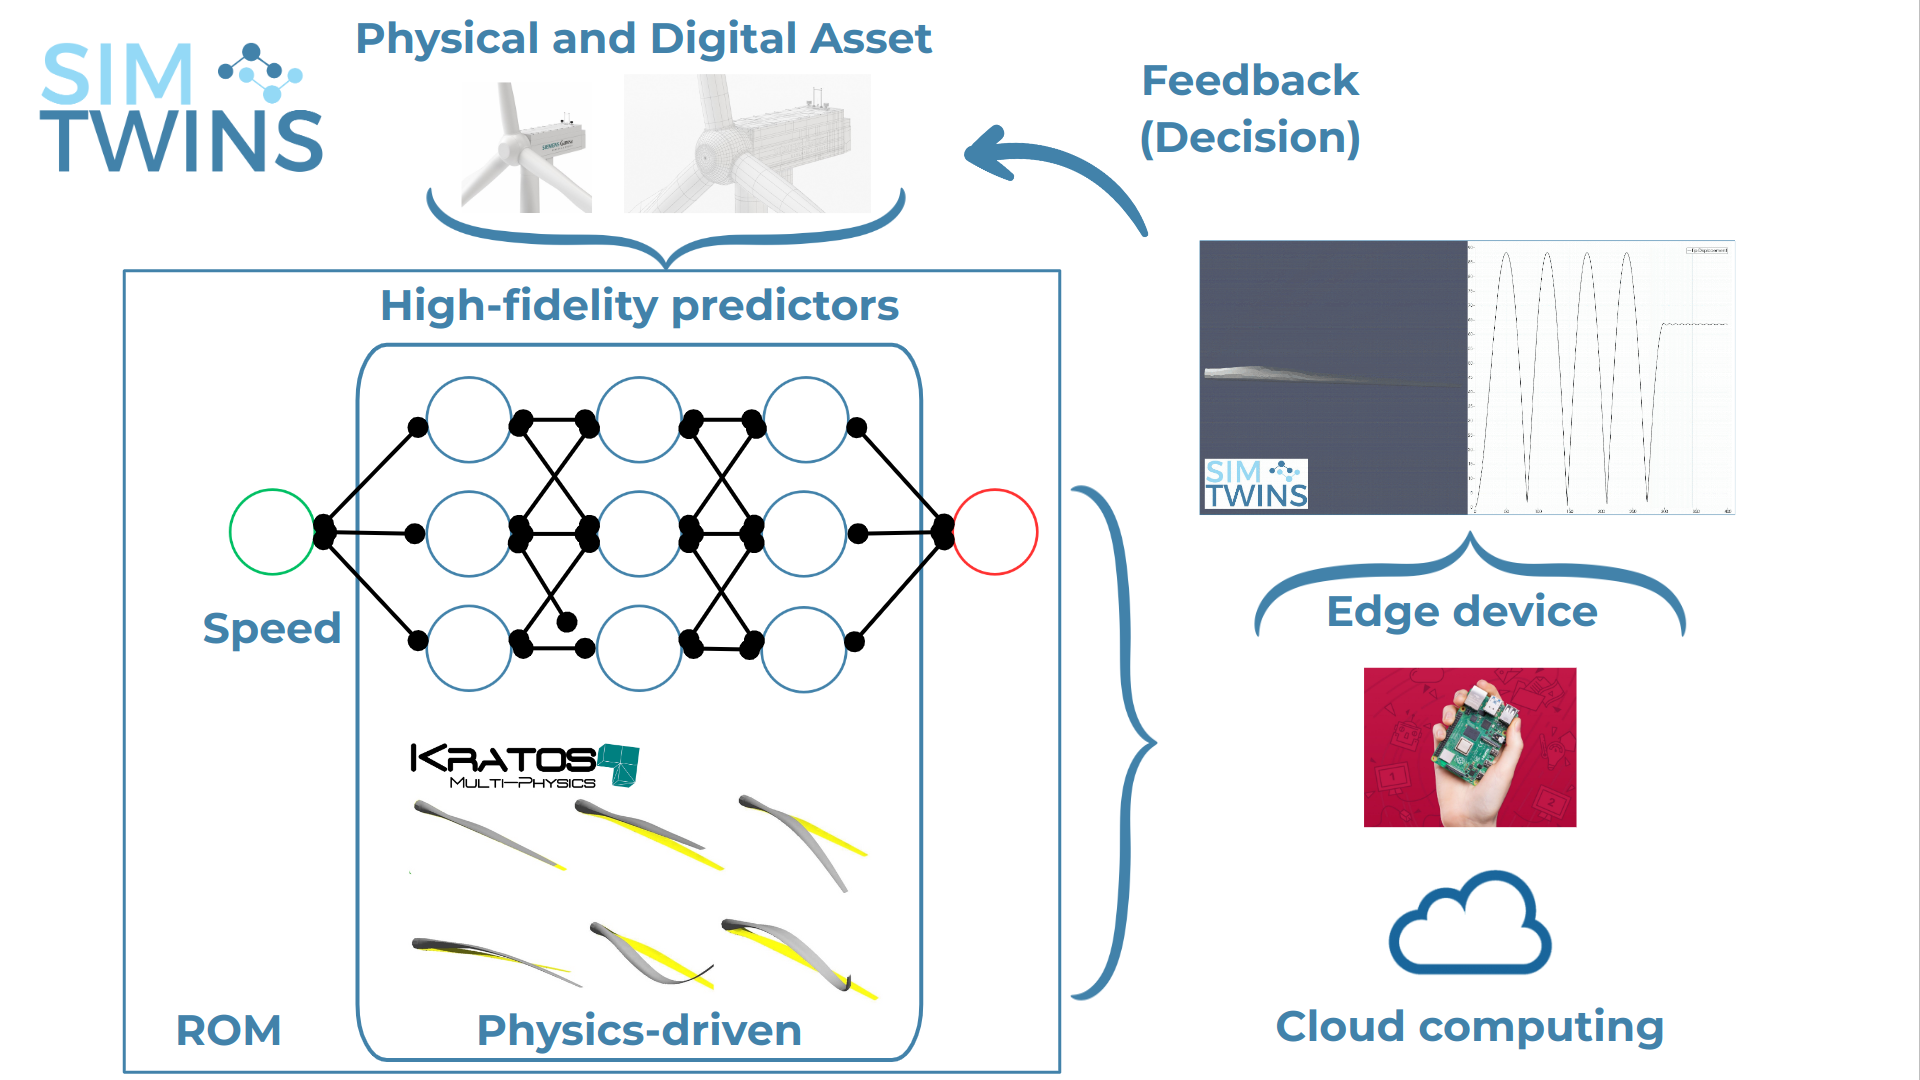
\includegraphics[trim=0mm 0mm 6mm 0mm, clip, width=0.92\textwidth]{Figures/DigitalTwinChartWindTurbine.png}
    \caption{Example of a wind turbine blade digital twin setup combining a physical asset, high-fidelity simulation-based predictors, and deployment across edge and cloud computing environments.}
    \label{fig:windturbine_digitaltwin}
\end{figure}

At the core of digital twins are simulation engines that replicate system behavior under varying conditions~\cite{hinchy2020using}. Despite their predictive power, high-fidelity simulations often demand substantial computational resources, constraining their practical application in scenarios that require rapid and repeated model evaluations. To address this challenge, ROMs have become integral components of digital twin technology. ROMs significantly reduce evaluation times and computational cost while preserving critical physical characteristics, enabling fast and accurate analyses required by digital twins~\cite{hartmann2018model, haas2012predictive}.

Among various ROM approaches, intrusive PROMs offer a compelling balance between accuracy, interpretability, and computational performance. Their preservation of the underlying physics and compatibility with advanced reduction methods make them especially suitable for digital twin applications in engineering. ROM-based digital twins are increasingly deployed via the \textit{Functional Mock-up Interface} (FMI) standard, which encapsulates ROMs into portable \textit{Functional Mock-up Units} (FMUs)~~\cite{blochwitz2011functional}. This approach enables seamless integration across diverse platforms and facilitates real-time interactions between simulations and operational systems. In this thesis, these concepts are consolidated into a parallel, scalable workflow designed explicitly for deploying ROM-based digital twins through FMUs in high-dimensional industrial scenarios~~\cite{Ares2024}.

Building upon these ideas, the present thesis proposes methodological advancements and robust implementation frameworks aimed at overcoming current limitations in ROM technologies. The subsequent sections formalize these motivations, outlining the specific research objectives and methodological approaches guiding this work.

\section{Approach and objectives}

To address the persistent gap between high-fidelity simulation capabilities and the real-time, scalable demands of modern digital twin applications, this thesis develops a cohesive framework for PROM that bridges the spectrum from simplified model problems to complex industrial scenarios. Recognizing that convection-dominated regimes, nonlinear dynamics, and extensive parametric studies pose significant challenges for conventional ROMs, this work systematically combines methodological advances in projection, hyper-reduction, nonlinear manifold closure, and HPC-enabled workflows.

The approach begins with the inviscid one-dimensional Burgers' equation, serving as a canonical model problem that clearly exposes the limitations of linear subspace approximations and motivates robust enhancements such as Petrov–Galerkin projection and residual-minimizing formulations. These insights are then scaled to more realistic engineering configurations, including the thermal dynamics of an electric motor within the eFlows4HPC context and the turbulent wake flow of the Ahmed body, a benchmark relevant to automotive industry aerodynamics, using Kratos Multiphysics and AERO-F. By embedding these developments within open-source platforms and implementing distributed training and hyper-reduction strategies, this thesis advances the practical deployment of PROMs for high-dimensional, real-time applications.

The specific objectives of this thesis are therefore to:
\begin{enumerate}
    \item Develop and assess linear projection-based ROMs (Galerkin, LSPG) for convection-dominated systems, using both canonical model problems and representative industry-like cases to characterize their performance and inherent limitations.
    \item Formulate and implement a novel hyper-reduction strategy for Petrov–Galerkin PROMs, enabling element-wise acceleration compatible with finite element assembly in Kratos Multiphysics.
    \item Design and validate a parallel HPC workflow for the scalable training and deployment of intrusive ROMs, demonstrated through an industrial digital twin application for motor thermal management within the eFlows4HPC framework.
    \item Advance physics consistency in neural-network-based manifolds through discrete physics-informed training strategies that align data-driven approximations with the residual behavior of the underlying numerical scheme.
    \item Extend the PROM methodology to nonlinear regimes by investigating latent-space closure strategies, including PROM-ANN and interpretable kernel-based surrogates (PROM-GPR, PROM-RBF), to mitigate the Kolmogorov $n$-width barrier, demonstrated on both model problems and more complex configurations such as the Ahmed body wake flow using AERO-F.
\end{enumerate}

Collectively, these objectives consolidate the thesis contributions toward robust, scalable, and physically consistent projection-based ROMs, enabling their practical use in high-dimensional, real-time digital twin applications for industrial contexts.

% \clearpage

% \section*{Nomenclature}

% \begin{tabular}{ll}
% HPC           & High-Performance Computing \\
% ROM           & Reduced Order Model \\
% PROM          & Projection-Based Reduced Order Model \\
% FOM           & Full Order Model \\
% POD           & Proper Orthogonal Decomposition \\
% RB            & Reduced Basis \\
% PGD           & Proper Generalized Decomposition \\
% PDE           & Partial Differential Equation \\
% FEM           & Finite Element Method \\
% SVD           & Singular Value Decomposition \\
% LSPG          & Least-Squares Petrov--Galerkin \\
% EIM           & Empirical Interpolation Method \\
% DEIM          & Discrete Empirical Interpolation Method \\
% GNAT          & Gauss--Newton with Approximated Tensors \\
% ECSW          & Energy-Conserving Sampling and Weighting \\
% ECM           & Empirical Cubature Method \\
% ANN           & Artificial Neural Network \\
% PINN          & Physics-Informed Neural Network \\
% DT            & Digital Twin \\
% FMU           & Functional Mock-up Unit \\
% FMI           & Functional Mock-up Interface \\
% UQ            & Uncertainty Quantification \\
% nn           & Number of retained POD modes \\
% nn-width     & Kolmogorov nn-width \\
% \end{tabular}


% CHAPTER 2 - Model Problem
\chapter{Model problem}
\label{sec:model_problem}

In this chapter, a simplified yet representative model problem is defined to facilitate the analysis, demonstration, and comparison of advanced PROM methodologies developed throughout this thesis. The chosen model is the inviscid one-dimensional Burgers' equation, a canonical nonlinear PDE that captures essential features of convection-dominated phenomena, including nonlinear wave propagation, steep gradients, and shock formation. Its simplified yet rich structure allows clear examination of these phenomena while remaining computationally tractable, making it particularly suitable as a benchmark for the PROM techniques introduced later.

The chapter is organized as follows. First, the inviscid one-dimensional Burgers' equation is introduced in both strong and weak forms, explicitly defining boundary conditions and parameterized source terms. Next, the equation is discretized primarily using the finite element method (FEM), providing details on spatial discretization, stabilization, time integration schemes, and nonlinear solver strategies. A comprehensive parametric analysis is then presented, highlighting the nonlinear dependence of the solution on key parameters. Subsequently, results from the FEM discretization are compared with solutions obtained from finite volume (FV) and finite difference (FD) methods. These alternative approaches, fully detailed in Appendices~\ref{appendix:fvm_burgers} and~\ref{appendix:fd_burgers}, reinforce the consistency and robustness of the numerical solutions obtained. The chapter concludes by identifying a generalized discrete residual formulation common to all discretizations, laying the foundational algebraic framework for the unified PROM methodologies developed in subsequent chapters.

\section{Inviscid one-dimensional Burgers' equation}

The inviscid Burgers' equation serves as an ideal model problem to systematically investigate the capabilities and limitations of reduced-order models in nonlinear, convection-dominated PDE contexts. Its relatively simple form provides an accessible yet rigorous intermediate step before tackling more complex equations, such as the compressible Euler or Navier–Stokes equations encountered in fluid dynamics, aerospace engineering, and related fields. The Burgers' equation notably encapsulates fundamental nonlinear phenomena, including wave steepening and shock formation, thus offering critical insights into the challenges faced by projection-based methods when applied to hyperbolic PDEs and nonlinear transport problems.

While primary attention is given to the finite element discretization, chosen for its direct compatibility with the Kratos Multiphysics framework, alternative discretizations via finite volume and finite difference methods are introduced to enable comprehensive validation. These additional discretizations respectively align with AERO-F and provide a straightforward computational framework for rapid testing and algorithmic development. Detailed numerical developments and validations across all three discretizations facilitate a rigorous assessment of projection-based model reduction techniques under diverse numerical frameworks.

The following sections detail the mathematical formulation, numerical treatments, and parametric analyses of the Burgers' equation, establishing the groundwork necessary for effective reduced-order modeling discussed in the subsequent chapters.


\subsection{Strong form}

The one-dimensional Burgers' equation with a source term is given by:
\begin{equation}
\frac{\partial u(x,t)}{\partial t} 
\;+\; 
u(x,t)\,\frac{\partial u(x,t)}{\partial x} 
\;=\; 
f(x,t),
\quad
\forall x \in [0, L], 
\quad
\forall t \in [0, T],
\end{equation}
where \( u(x,t) \) denotes the velocity field, \( f(x,t) \) is a prescribed source term, \( L \) is the length of the spatial domain, and \( T \) is the final simulation time.

The governing equation is supplemented by the following boundary and initial conditions:
\begin{equation}
\begin{aligned}
&u(0, t) = u_{\text{left}}(t) = \mu_1, 
&&\quad \forall t \in [0, T], \\
&u(x, 0) = u_{\text{initial}}(x) = 1, 
&&\quad \forall x \in [0, L],
\end{aligned}
\end{equation}
where $\mu_1$ is a parameter controlling the Dirichlet inflow boundary condition at the left end of the domain.

The source term $f(x,t)$ is defined as:
\begin{equation}
f(x,t) = 0.02 \, e^{\mu_2 x},
\end{equation}
where $\mu_2$ is a spatial parameter that modulates the exponential growth of the source along the domain.

\subsection{Weak form}

To derive the weak form of the one-dimensional Burgers' equation with a source term, consider its strong form:
\begin{equation}
\frac{\partial u(x,t)}{\partial t} 
\;+\;
u(x,t) \,\frac{\partial u(x,t)}{\partial x}
\;=\;
f(x,t).
\end{equation}

Multiplying both sides by a test function \(v(x)\) and integrating over the spatial domain \([0, L]\) yields:
\begin{equation}
\int_0^L 
\Bigl(
\frac{\partial u}{\partial t}
\;+\;
u\,\frac{\partial u}{\partial x}
\;-\;
f(x,t)
\Bigr) 
\,v(x)\,\mathrm{d}x 
\;=\; 
0.
\end{equation}

Since there is no diffusion term, no integration by parts is required. The resulting weak form is therefore:
\begin{equation}
\int_0^L 
\Bigl(
\frac{\partial u}{\partial t}\,v
\;+\;
u\,\frac{\partial u}{\partial x}\,v
\Bigr)\,\mathrm{d}x
\;=\;
\int_0^L 
f(x,t)\,v\,\mathrm{d}x.
\end{equation}

This variational formulation must be satisfied by all admissible test functions \(v(x)\) in an appropriate Sobolev space (e.g.\ \(H_0^1([0,L])\)).

% \paragraph{Remark on non-homogeneous boundaries.}
% Strictly speaking, the above derivation assumes homogeneous Dirichlet boundary conditions if one requires \(v\) to vanish on \(\partial \Omega\). When dealing with non-homogeneous boundaries (e.g., \(u(0,t)=\mu_1\neq0\)), a common practice is to shift the unknown or incorporate the boundary data directly into the finite element basis, ensuring that the test functions still vanish on \(\partial \Omega\). This approach preserves the same weak formulation while properly enforcing the non-homogeneous boundary conditions in practice.

\section{Finite element discretization}
\label{sec:fem_discretization}
\subsection{Spatial discretization}

To numerically solve the weak form of the one-dimensional Burgers' equation, the spatial domain \([0, L]\) is subdivided into \(N_e\) finite elements with nodes \(x_i\), \(i = 1, \dots, N\), where \(N = N_e\ + 1\) is the total number of nodes.

The solution \(u(x,t)\) and the test function \(v(x)\) are approximated using standard finite element basis functions \(N_j(x)\) as
\begin{equation}
u(x,t) \;\approx\; \sum_{j=1}^{N} u_j(t)\,N_j(x), 
\quad 
v(x) \;=\; N_i(x),
\end{equation}
where \(u_j(t)\) denotes the time-dependent nodal values and \(N_j(x)\) are the associated shape functions.

Substituting these approximations into the weak form of the inviscid Burgers' equation with source term 
\begin{equation}
\int_0^L 
\Bigl(\,
\tfrac{\partial u}{\partial t}
\;+\;
u\,\tfrac{\partial u}{\partial x}
\;-\;
f(x,t)
\Bigr)\,v\,\mathrm{d}x
\;=\;
0
\end{equation}
yields the following semi-discrete system:
\begin{equation}
\begin{split}
\sum_{j=1}^{N} \frac{du_j(t)}{dt} 
\int_0^L 
N_j(x)\,N_i(x)\,\mathrm{d}x
\;+\;
\sum_{j=1}^{N} 
u_j(t)
\int_0^L 
\Bigl(\sum_{k=1}^{N} u_k(t)\,N_k(x)\Bigr)
\frac{\partial N_j(x)}{\partial x}\,N_i(x)\,\mathrm{d}x
\\
\;=\;
\int_0^L 
f(x,t)\,N_i(x)\,\mathrm{d}x.
\end{split}
\label{eq:standard_semidiscrete}
\end{equation}

This formulation leads naturally to the following mass matrix \(\mathbf{M}\), nonlinear convection matrix \(\mathbf{C}(\mathbf{u})\), and load vector \(\mathbf{F}(t)\):
\begin{subequations}
\begin{align}
M_{ij} &\;=\; \int_0^L N_i(x)\,N_j(x)\,\mathrm{d}x,
\\
C_{ij}(\mathbf{u}) &\;=\; \int_0^L 
\Bigl(\sum_{k=1}^{N} u_k(t)\,N_k(x)\Bigr) 
\frac{\partial N_j(x)}{\partial x}\,N_i(x)\,\mathrm{d}x,
\\
F_i(t) &\;=\; \int_0^L f(x,t)\,N_i(x)\,\mathrm{d}x.
\end{align}
\end{subequations}

Collecting these elements into matrix form provides a (nonlinear) ordinary differential equation (ODE):
\begin{equation}
\mathbf{M} \,\frac{d\mathbf{u}(t)}{dt} 
\;+\;
\mathbf{C}\bigl(\mathbf{u}(t)\bigr)\,\mathbf{u}(t)
\;=\;
\mathbf{F}(t),
\end{equation}
where \(\mathbf{u}(t) \in \mathbb{R}^N\) is the vector of nodal unknowns. The nonlinearity stems from the convective term \(\mathbf{C}(\mathbf{u})\). %Appropriate boundary conditions are enforced by modifying the system matrix and right-hand side.

\subsection{SUPG stabilization}

In purely convective or convection-dominated regimes, the standard Galerkin approach described in \eqref{eq:standard_semidiscrete} may suffer from spurious oscillations. To address this, a \textit{Streamline-Upwind/Petrov--Galerkin} (SUPG) term can be added to the spatial discretization. In the one-dimensional case, the SUPG weak form augments the integral with a residual-based term aligned with the flow direction:
\begin{equation}
\int_0^L 
\Bigl(
\tfrac{\partial u}{\partial t} + u\,\tfrac{\partial u}{\partial x} - f
\Bigr)\,v
\,\mathrm{d}x
\;+\;
\sum_{e=1}^{N_e} 
\int_{\Omega_e} 
\tau_e \,
\Bigl(u\,\tfrac{\partial u}{\partial x} - f\Bigr)\,
\frac{\partial v}{\partial x}
\,\mathrm{d}x
\;=\;
0,
\end{equation}
where \(\Omega_e\) denotes the physical domain of element \(e\) and  \(\tau_e\) is an elementwise stabilization parameter (e.g.\ \(\tau_e \sim \tfrac{h_e}{2\,|u|}\) in one-dimensional). After discretization in finite elements, this introduces an additional stabilization vector \(\mathbf{S}\bigl(\mathbf{u}\bigr)\) that modifies the final ODE system to:
\begin{equation}
\mathbf{M} \,\frac{d\mathbf{u}(t)}{dt} 
\;+\;
\mathbf{C}\bigl(\mathbf{u}\bigr)\,\mathbf{u}(t)
\;+\;
\mathbf{S}\bigl(\mathbf{u}(t)\bigr)
\;=\;
\mathbf{F}(t).
\end{equation}

With this stabilized spatial discretization in place, the system is now ready for a suitable time integration scheme, as discussed in the subsequent section.


\subsection{Time discretization}

Let \(\Delta t\) denote the time step, and define \(\mathbf{u}^n\) as the solution at \(t^n = n\,\Delta t\). For simplicity, a first-order accurate \textit{Backward Euler method} is adopted here, due to its stability properties in convection-dominated problems. In the presence of SUPG stabilization, the resulting fully discrete equation at each time step \(n\) becomes:
\begin{equation}
\mathbf{M} \,\frac{\mathbf{u}^{n+1} - \mathbf{u}^n}{\Delta t}
\;+\;
\mathbf{C}\bigl(\mathbf{u}^{n+1}\bigr)\,\mathbf{u}^{n+1}
\;+\;
\mathbf{S}\bigl(\mathbf{u}^{n+1}\bigr)
\;=\;
\mathbf{F}^{n+1},
\label{eq:BE_supg_inviscid}
\end{equation}
where \(\mathbf{M}\) is the mass matrix, \(\mathbf{C}\bigl(\mathbf{u}^{n+1}\bigr)\) denotes the nonlinear convection operator, \(\mathbf{S}\bigl(\mathbf{u}^{n+1}\bigr)\) represents the SUPG stabilization vector, and \(\mathbf{F}^{n+1}\) is the load vector at the new time level. Because of the nonlinear convective term and the dependence of \(\mathbf{S}\) on \(\mathbf{u}^{n+1}\), a nonlinear system must be solved at each time step.

A second-order accurate alternative, often referred to as the \textit{Crank--Nicolson method}, is discussed in Appendix~\ref{appendix:cranknicolson}.

\subsection{Defining the residual}

Once the system is discretized in both space and time using \eqref{eq:BE_supg_inviscid}, the resulting nonlinear algebraic equation at each time step \(n\) can be rearranged to define a \textit{residual} 
\(\mathbf{R}\bigl(\mathbf{u}^{n+1}\bigr)\). Specifically,
\begin{equation}
\mathbf{R}\bigl(\mathbf{u}^{n+1}\bigr) 
\;=\;
\mathbf{M}\,\frac{\mathbf{u}^{n+1} - \mathbf{u}^n}{\Delta t} 
\;+\;
\mathbf{C}\bigl(\mathbf{u}^{n+1}\bigr)\,\mathbf{u}^{n+1} 
\;+\;
\mathbf{S}\bigl(\mathbf{u}^{n+1}\bigr)
\;-\;
\mathbf{F}^{n+1}.
\label{eq:R_supg_inviscid}
\end{equation}
Equivalently, one may write
\begin{equation}
\mathbf{R}\bigl(\mathbf{u}^{n+1}\bigr) 
\;=\;
\mathbf{A}\bigl(\mathbf{u}^{n+1}\bigr)\,\mathbf{u}^{n+1} 
\;-\;
\mathbf{b}^{n+1}
\;+\;
\mathbf{S}\bigl(\mathbf{u}^{n+1}\bigr),
\label{eq:R_full_inviscid}
\end{equation}
where 
\begin{equation}
\mathbf{A}\bigl(\mathbf{u}^{n+1}\bigr) 
\;=\;
\mathbf{M} 
\;+\;
\Delta t\,\mathbf{C}\bigl(\mathbf{u}^{n+1}\bigr),
\quad
\mathbf{b}^{n+1} 
\;=\;
\mathbf{M}\,\mathbf{u}^n 
\;+\;
\Delta t\,\mathbf{F}^{n+1}.
\end{equation}
Since \(\mathbf{S}\bigl(\mathbf{u}^{n+1}\bigr)\) also depends on the unknown solution, the final system remains fully nonlinear. The vector \(\mathbf{R}\bigl(\mathbf{u}^{n+1}\bigr)\) measures the mismatch between the left- and right-hand sides of the fully discrete equation, and the objective is to find \(\mathbf{u}^{n+1}\) such that 
\(\mathbf{R}\bigl(\mathbf{u}^{n+1}\bigr) = \boldsymbol{0}\).

\subsection{Residual minimization via nonlinear solvers}

Once the fully discrete system 
\begin{equation}
\mathbf{R}\bigl(\mathbf{u}^{n+1}\bigr) 
\;=\;
\boldsymbol{0},
\label{eq:residual_fem}
\end{equation}
is formed (for instance, from a Backward Euler discretization with SUPG stabilization), the objective is to find \(\mathbf{u}^{n+1}\) such that the residual \(\mathbf{R}\) vanishes at each time step. Two prominent approaches for solving this nonlinear system are the \textit{Newton--Raphson method} and the \textit{Picard} (fixed-point) iteration method.

\paragraph{Newton--Raphson method}

In the Newton--Raphson method, the residual is expanded in a first-order Taylor series around the current iterate \(\mathbf{u}^{(k)}\), yielding
\begin{equation}
\mathbf{R}\bigl(\mathbf{u}^{(k+1)}\bigr)
\,\approx\,
\mathbf{R}\bigl(\mathbf{u}^{(k)}\bigr)
\;+\;
\mathbf{J}\bigl(\mathbf{u}^{(k)}\bigr)\,
\Bigl(\mathbf{u}^{(k+1)} - \mathbf{u}^{(k)}\Bigr),
\end{equation}
where \(\mathbf{J}\bigl(\mathbf{u}^{(k)}\bigr) = \tfrac{\partial \mathbf{R}}{\partial \mathbf{u}}\) is the \textit{Jacobian matrix} of partial derivatives evaluated at \(\mathbf{u}^{(k)}\). By enforcing
\(\mathbf{R}\bigl(\mathbf{u}^{(k+1)}\bigr)=\boldsymbol{0},\) one obtains the standard Newton update:
\begin{subequations}
\begin{align}
\mathbf{J}\bigl(\mathbf{u}^{(k)}\bigr)\,\delta \mathbf{u}^{(k)} 
&=\;
-\,\mathbf{R}\bigl(\mathbf{u}^{(k)}\bigr),\\
\mathbf{u}^{(k+1)} 
&=\;
\mathbf{u}^{(k)}
\;+\;
\delta \mathbf{u}^{(k)},
\end{align}
\end{subequations}
where \(\delta \mathbf{u}^{(k+1)}\) is the correction term. Provided that \(\mathbf{u}^{(k)}\) is sufficiently close to the true solution, Newton--Raphson typically converges \textit{quadratically}, meaning the error is reduced very rapidly with each iteration. However, computing or assembling the full Jacobian \(\mathbf{J}\) can be expensive, especially if the nonlinear terms involve complex operators (e.g., \(\mathbf{C}(\mathbf{u})\) and the SUPG stabilization vector \(\mathbf{S}(\mathbf{u})\)) that depend intricately on \(\mathbf{u}\).

\paragraph{Picard (fixed-point) iteration}

Picard iteration offers a simpler approach in which the Jacobian is approximated by a \emph{frozen} or \emph{simplified} operator. In many convection-dominated problems, one may treat the convective and SUPG terms as if they are constant with respect to \(\mathbf{u}\) (or use a partial linearization). Concretely, Picard iteration can be written in the same two-step form:
\begin{subequations}
\begin{align}
\mathbf{A}\bigl(\mathbf{u}^{(k)}\bigr)\,\delta \mathbf{u}^{(k)}
&=\;
-\,\mathbf{R}\bigl(\mathbf{u}^{(k)}\bigr),
\\
\mathbf{u}^{(k+1)} 
&=\;
\mathbf{u}^{(k)} 
\;+\;
\delta \mathbf{u}^{(k)}.
\end{align}
\end{subequations}
but now the \emph{iteration matrix} \(\mathbf{A}\bigl(\mathbf{u}^{(k)}\bigr)\) is chosen to be a simpler approximation to the true derivative \(\mathbf{J}\). For instance, \(\mathbf{A}\) might come from freezing the convection matrix \(\mathbf{C}\) and SUPG term \(\mathbf{S}\) at the old iterate. This often makes each iteration cheaper and can be more robust if the initial guess is far from the solution, but at the expense of slower convergence than Newton--Raphson.

\paragraph{Comparison and practical usage}

Both methods share a common framework of linear updates:
\begin{equation}
\mathbf{J}\bigl(\mathbf{u}^{(k)}\bigr)\,\delta\mathbf{u}^{(k)}
\;=\;
-\,\mathbf{R}\bigl(\mathbf{u}^{(k)}\bigr),
\end{equation}
with the distinction that in \textbf{Newton--Raphson} the Jacobian \(\mathbf{J}\) is computed from the exact derivative of all nonlinear terms (including SUPG), whereas in \textbf{Picard iteration} one substitutes a simpler operator, such as the system matrix \(\mathbf{A}\bigl(\mathbf{u}^{(k)}\bigr)\) or even a partially linearized version. Consequently:
\begin{itemize}
    \item \textbf{Newton--Raphson} converges faster \textit{(often quadratically)} if the Jacobian is well-defined and the solution guess is reasonably close;
    \item \textbf{Picard iteration} is easier to implement and more robust for large or uncertain initial guesses, but often converges more slowly.
\end{itemize}

In many convection-dominated PDE codes, Picard iteration is favored for its balance of simpler assembly (avoiding the full partial derivatives of \(\mathbf{C}(\mathbf{u})\mathbf{u}\) and \(\mathbf{S}(\mathbf{u})\)). Newton--Raphson remains valuable when rapid convergence is critical or when the cost of each iteration is not prohibitively large. For the present study, the Picard approach is employed, referring to its iteration matrix generically as \(\mathbf{J}\), even though it may not be the exact derivative of the residual.

\section{Numerical results and assesment}

This subsection presents and analyzes numerical results obtained from simulations of the one-dimensional inviscid Burgers' equation. These experiments involve varying key parameters such as the inflow boundary condition parameter (\(\mu_1\)) and the source-term parameter (\(\mu_2\)). The evolution of the solution over time is systematically examined, emphasizing characteristic phenomena such as shock formation, wave propagation speed, and nonlinear effects.

The performance and accuracy of the finite element discretization presented in this chapter are directly compared against the finite volume and finite difference implementations detailed in Appendices~\ref{appendix:fvm_burgers} and~\ref{appendix:fd_burgers}. The spatial domain \([0, 100]\) is discretized using 511 linear finite elements, resulting in 512 nodes and thus 512 spatial degrees of freedom for the finite element model. This nodal discretization aligns with the Galerkin formulation introduced in Section~\ref{sec:fem_discretization}. Equivalent resolutions are adopted for the comparison schemes: the finite volume method employs 512 control volumes centered at equally spaced locations in the domain, while the finite difference scheme uses 512 uniformly spaced nodes. This consistent spatial resolution across all methods ensures fair numerical comparisons and enables consistent offline–online decomposition for the reduced-order models.

This comparative analysis underscores the consistency and robustness of the proposed discretizations and serves as validation for the subsequent reduced-order modeling strategies explored in later chapters. 

\subsection{Parametric sensitivity}

To investigate how the dynamics of the one-dimensional inviscid Burgers' equation respond to changes in boundary and source parameters, a structured parametric study is performed using the high-fidelity finite element model developed in this chapter. This analysis lays the groundwork for understanding the structure of the solution manifold and its dependence on input parameters, an essential step before constructing any reduced-order model.

The study considers the following cases:

\begin{itemize}
    \item \textbf{Varying the inflow parameter \(\mu_1\)} while keeping the source parameter fixed at \(\mu_2 = 0.0225\). We explore three representative values: \(\mu_1 = 4.250\), \(4.875\), and \(5.500\).
    \item \textbf{Varying the source parameter \(\mu_2\)} while keeping the inflow parameter fixed at \(\mu_1 = 4.875\). We consider \(\mu_2 = 0.0150\), \(0.0225\), and \(0.0300\).
\end{itemize}

To visualize the transient dynamics, both 3D surface plots of the solution \(u(x,t)\) and 2D time-slice profiles at selected snapshots \(t = \{5, 10, 15, 20\}\,\text{s}\) are generated. These results are presented in Figures~\ref{fig:3d_parametric}--\ref{fig:subplots_mu2_fixed_mu1}.

\vspace{0.5em}
\noindent The key observations are:

\begin{itemize}
    \item Increasing \(\mu_1\) (with \(\mu_2 = 0.0225\) fixed) leads to faster wavefront propagation, steeper shock gradients, and higher early-time amplitudes.
    \item Increasing \(\mu_2\) (with \(\mu_1 = 4.875\) fixed) amplifies the effect of the exponential source term, significantly raising the downstream solution over time.
\end{itemize}

These experiments reveal how each parameter affects both the magnitude and shape of the evolving wavefront. The results confirm that the system exhibits strong nonlinear dependence on both \(\mu_1\) and \(\mu_2\), with the influence of \(\mu_1\) being more prominent during early time evolution and \(\mu_2\) dominating the late-time response.

\begin{figure}[htbp]
    \centering
    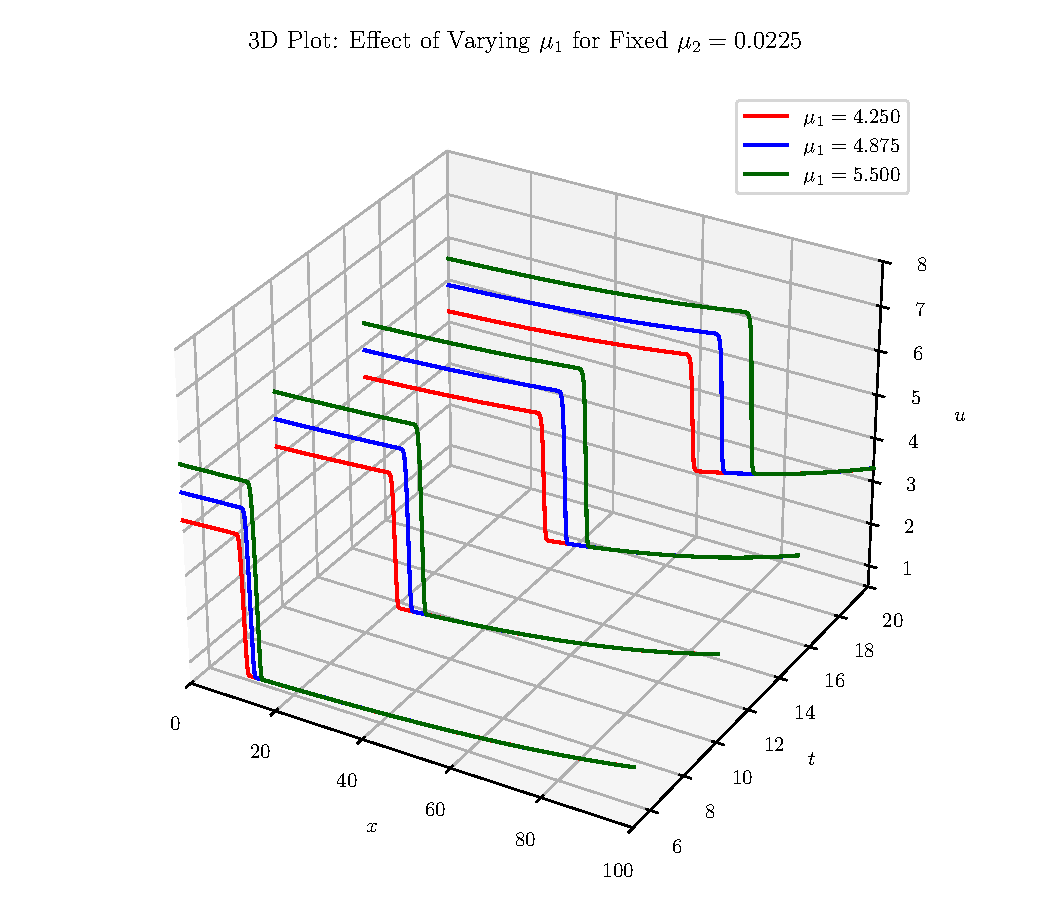
\includegraphics[width=0.45\textwidth]{Figures/plot_mu1_variation.pdf}
    \hfill
    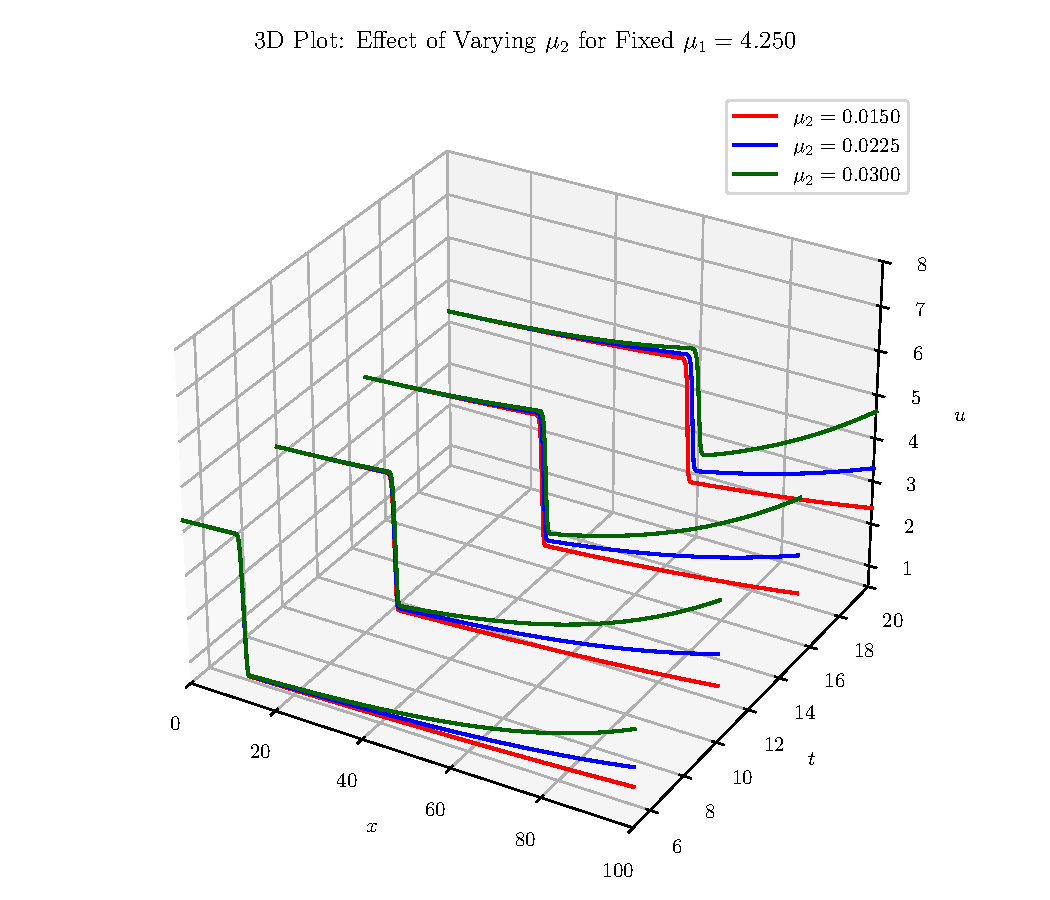
\includegraphics[width=0.45\textwidth]{Figures/plot_mu2_variation.pdf}
    \caption{3D plots of the full-order solution \(u(x,t)\). \textbf{Left:} Varying \(\mu_1 \in \{4.250, 4.875, 5.500\}\) with fixed \(\mu_2 = 0.0225\). \textbf{Right:} Varying \(\mu_2 \in \{0.0150, 0.0225, 0.0300\}\) with fixed \(\mu_1 = 4.875\).}
    \label{fig:3d_parametric}
\end{figure}

\begin{figure}[htbp]
    \centering
    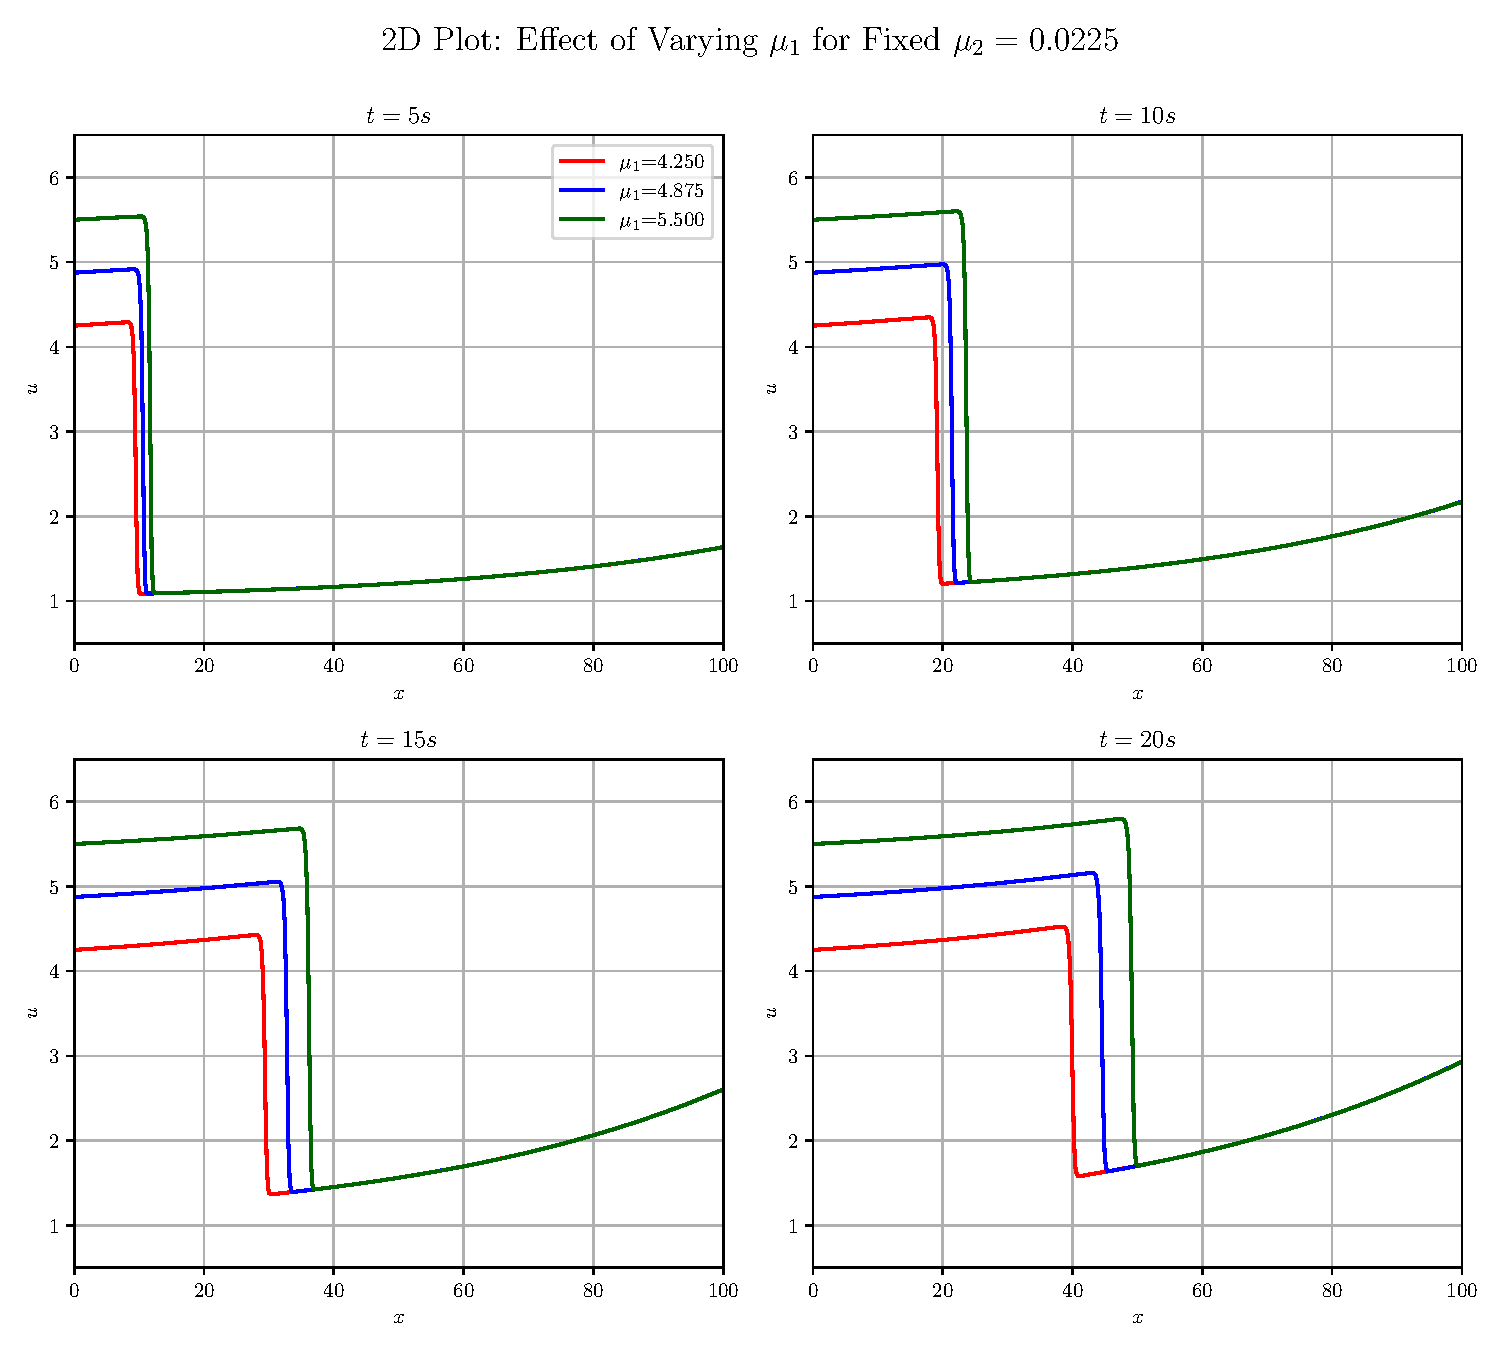
\includegraphics[width=0.65\textwidth]{Figures/subplot_mu1_variation.pdf}
    \caption{2D time-slice profiles at \(t = \{5,10,15,20\}\) seconds for different \(\mu_1\) values, with \(\mu_2 = 0.0225\) fixed.}
    \label{fig:subplots_mu1_fixed_mu2}
\end{figure}

\begin{figure}[htbp]
    \centering
    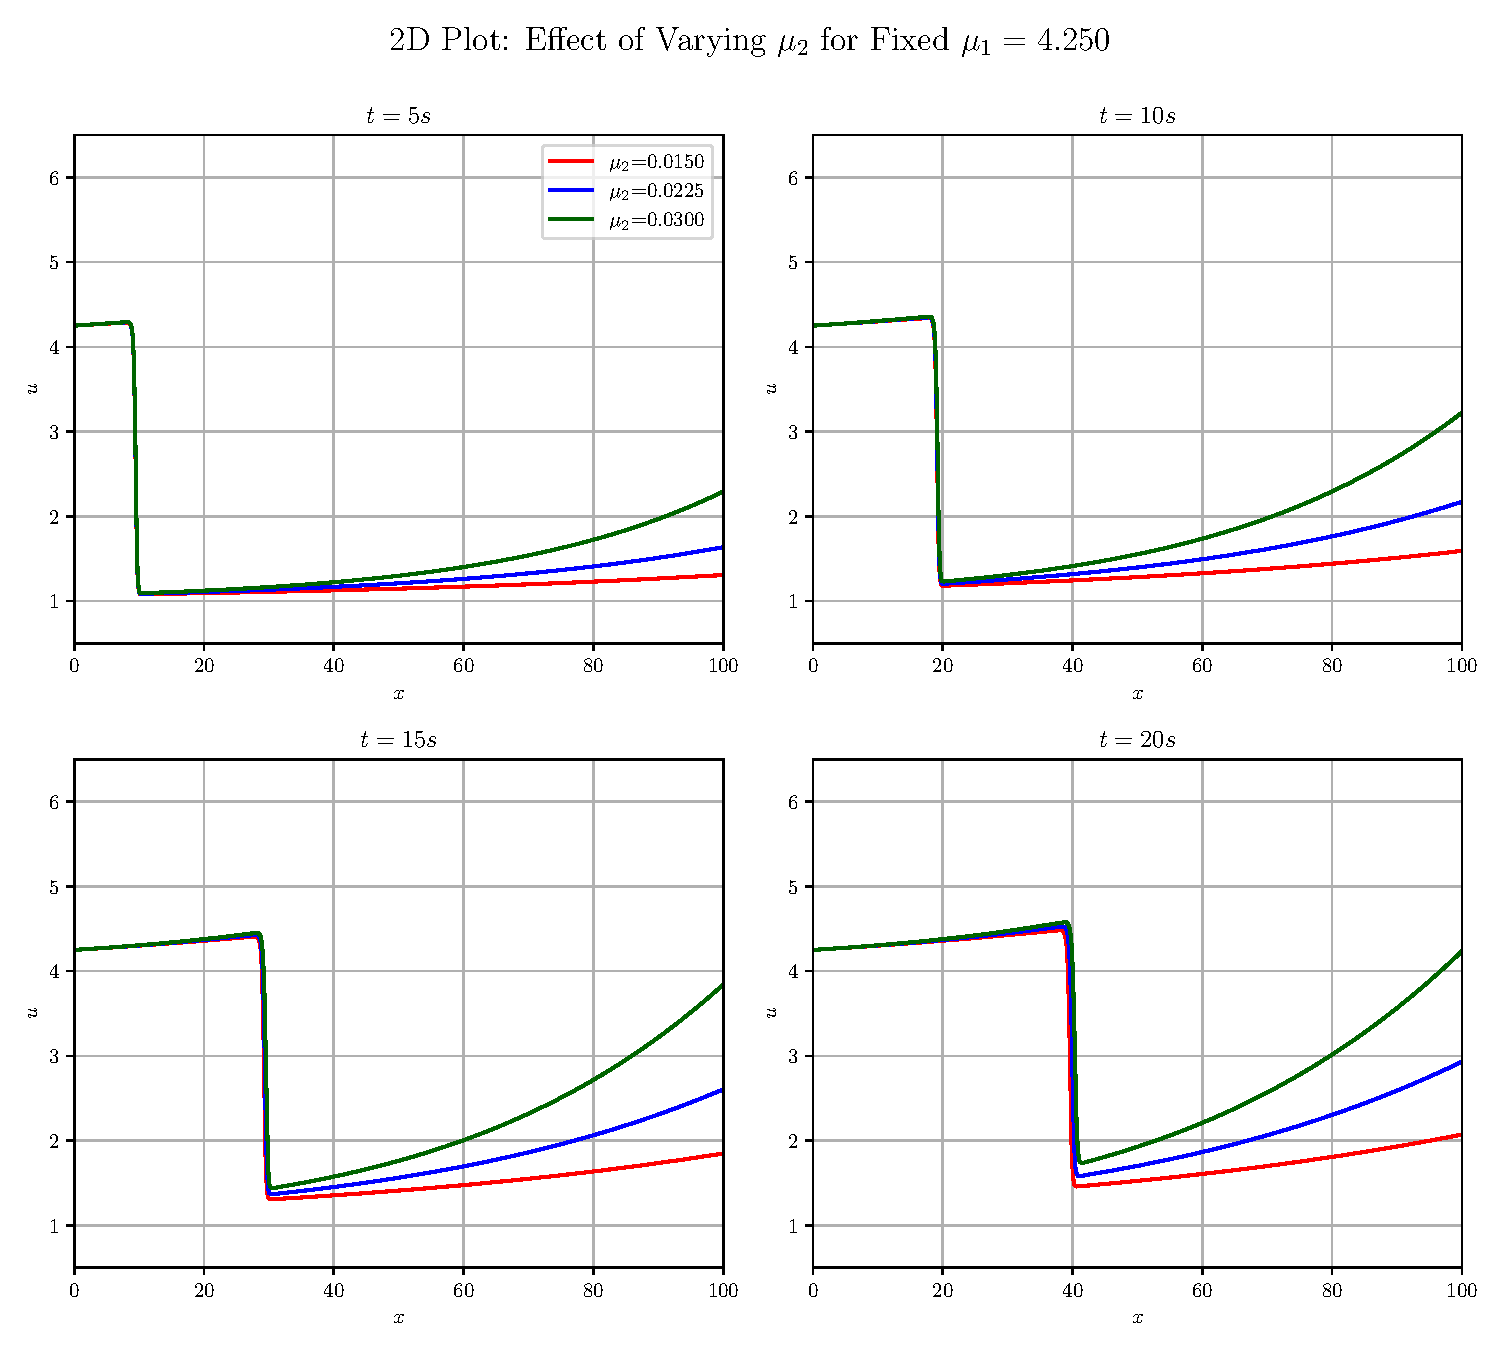
\includegraphics[width=0.65\textwidth]{Figures/subplot_mu2_variation.pdf}
    \caption{2D time-slice profiles at \(t = \{5,10,15,20\}\) seconds for different \(\mu_2\) values, with \(\mu_1 = 4.875\) fixed.}
    \label{fig:subplots_mu2_fixed_mu1}
\end{figure}

Since full 3D or multi-panel 2D visualizations are impractical for repeated comparison, Figure~\ref{fig:overlay_mu1_4875_mu2_0225} provides a compact view of the solution evolution by overlaying selected time instants for a representative parameter configuration. This will serve as a reference for subsequent comparisons across discretization methods and reduced-order approximations.

\begin{figure}[htbp]
    \centering
    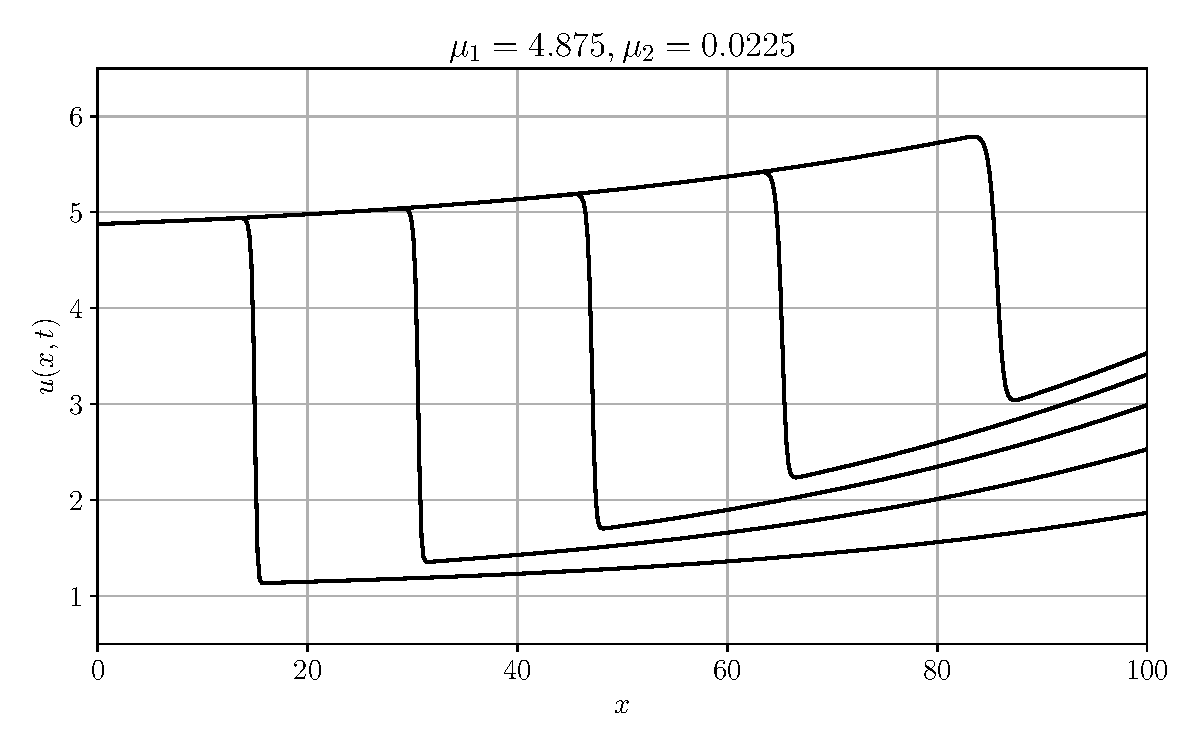
\includegraphics[width=0.7\textwidth]{Figures/overlayed_fom_mu1_4.875_mu2_0.0225.pdf}
    \caption{
    Overlay of the velocity field \( u(x,t) \) at several time instants for parameter configuration \( \bm{\mu} = [4.875,\; 0.0225] \). 
    The selected snapshots illustrate the evolution of the nonlinear wave profile at \( t = 5,\,10,\,15,\,20,\,25\,\text{s} \). 
    This compact visualization is used to qualitatively assess solution features such as steepening fronts and overall transport behavior. 
    Labels are omitted to keep the plot clean for later comparisons between discretization strategies and reduced-order models.
    }
    \label{fig:overlay_mu1_4875_mu2_0225}
\end{figure}

\subsection{Comparison across discretization methods}

To validate the finite element formulation introduced in this chapter and to benchmark its performance, its results are compared against two alternative discretization strategies: finite volume and finite difference. These additional implementations are described in detail in Appendices~\ref{appendix:fvm_burgers} and~\ref{appendix:fd_burgers}, respectively.

The comparison is conducted for two representative parameter configurations:
\begin{itemize}
    \item \(\bm{\mu}_\text{A} = [4.250,\; 0.0150]\): low inflow and mild source;
    \item \(\bm{\mu}_\text{B} = [5.500,\; 0.0300]\): high inflow and steep source.
\end{itemize}

Figure~\ref{fig:discretization_comparison_muA} and Figure~\ref{fig:discretization_comparison_muB} present overlayed plots of the velocity field at selected time instants for each method. In all cases, the same initial and boundary conditions, source term, and time stepping scheme are used to ensure a fair comparison.

Overall, the three methods exhibit excellent qualitative agreement in wave propagation and steepening behavior. Minor differences are observed in the sharpness of the wave front and dissipation characteristics. These discrepancies can be attributed to differences in numerical diffusion, order of accuracy, and stabilization mechanisms inherent to each scheme.

For the remainder of this chapter, the finite element method is adopted as the baseline discretization for the model problem. This choice is motivated by its alignment with the Kratos Multiphysics framework, which supports the broader reduced-order modeling developments presented in the thesis. Nevertheless, the finite difference implementation proved invaluable during early-stage algorithmic development and testing due to its simplicity and flexibility. Furthermore, the finite volume is revisited in Chapter~\ref{chap:article4}, where it is employed in the context of nonlinear subspace reduced-order models through its integration with the AERO-F platform.

\begin{figure}[htbp]
    \centering
    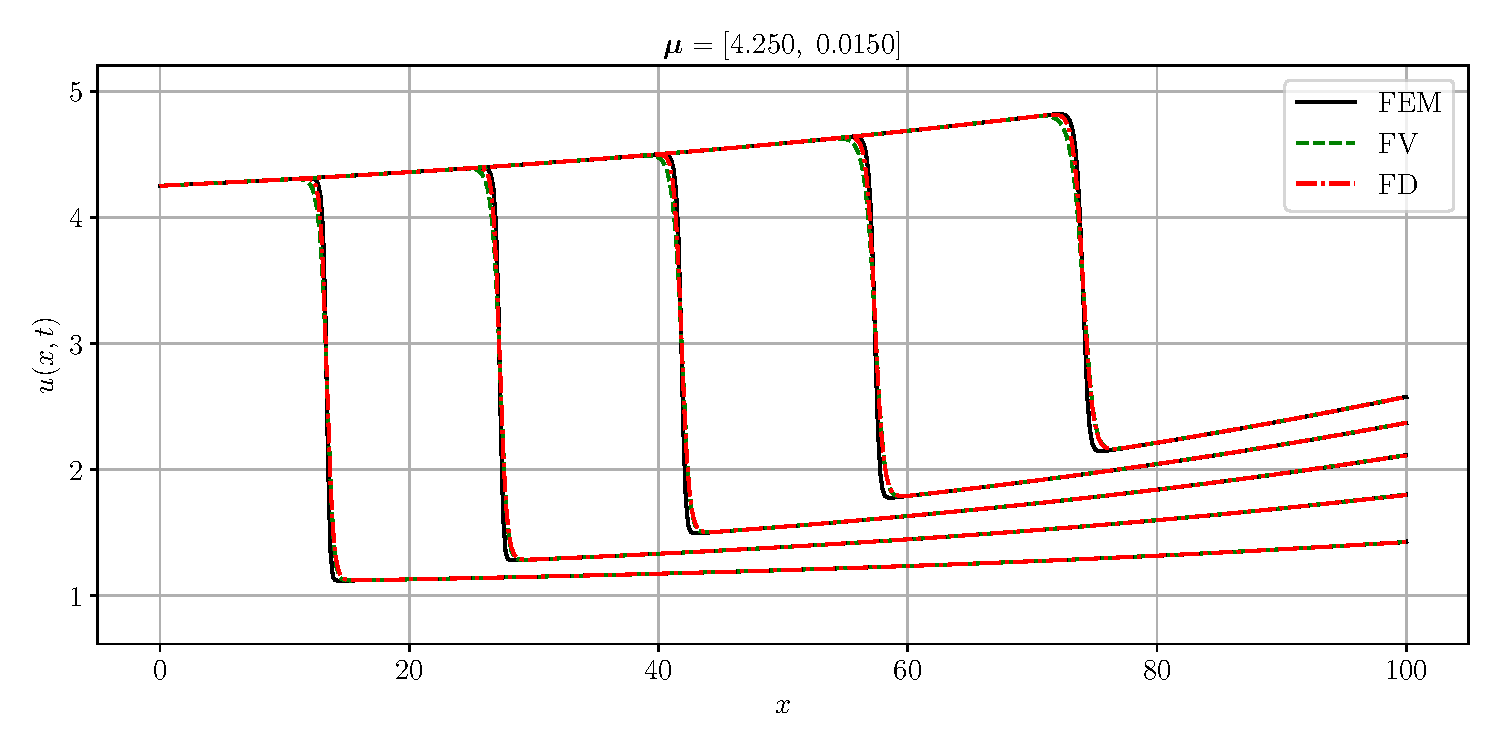
\includegraphics[width=0.7\textwidth]{Figures/discretization_comparison_overlay_mu1_4.250_mu2_0.0150.pdf}
    \caption{
    Comparison of FEM, FV, and FD results for parameter configuration \(\bm{\mu}_\text{A} = [4.250,\; 0.0150]\).
    The figure shows overlayed velocity profiles at multiple time instants.
    All methods produce consistent solutions, with minor variations in wave steepness and dissipation due to numerical differences.
    }
    \label{fig:discretization_comparison_muA}
\end{figure}

\begin{figure}[htbp]
    \centering
    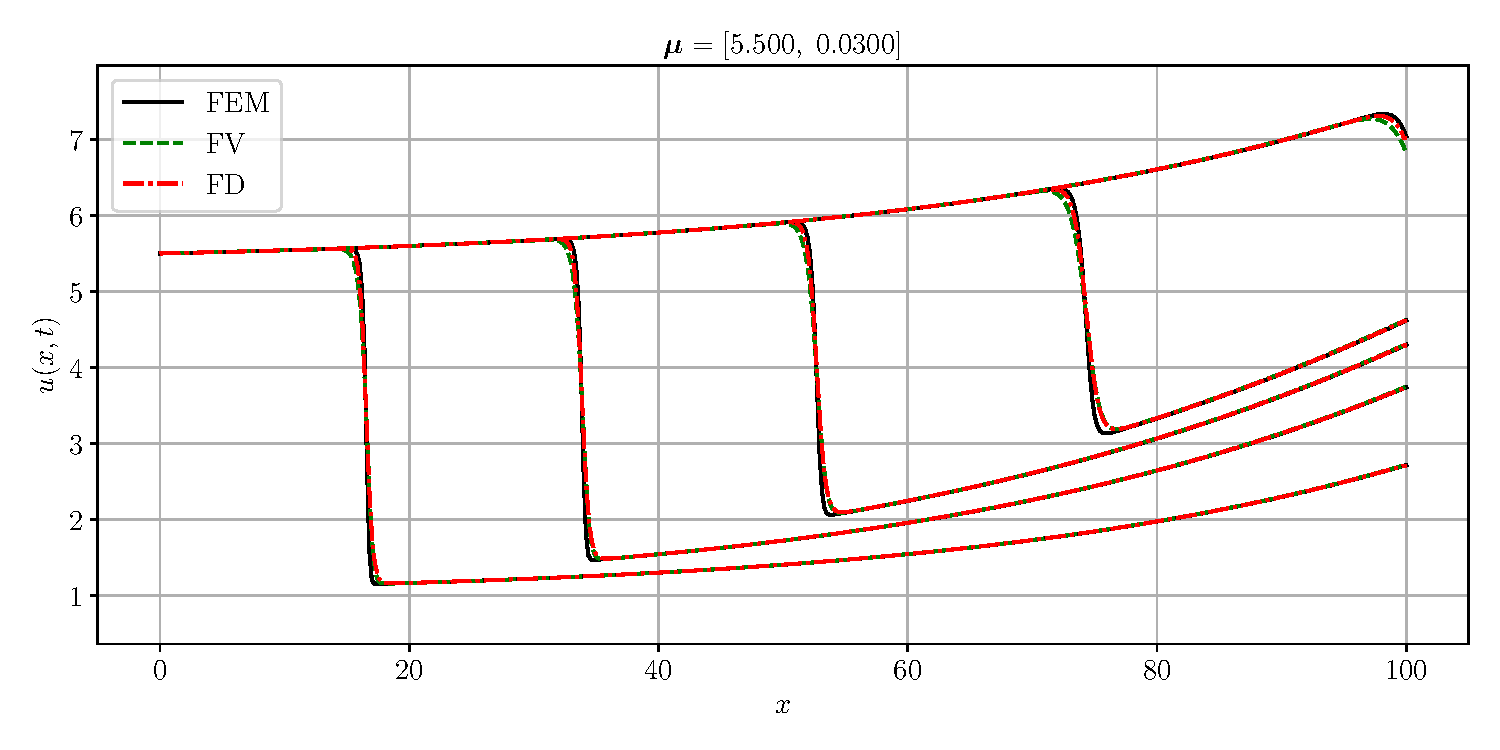
\includegraphics[width=0.7\textwidth]{Figures/discretization_comparison_overlay_mu1_5.500_mu2_0.0300.pdf}
    \caption{
    Comparison of FEM, FV, and FD results for parameter configuration \(\bm{\mu}_\text{B} = [5.500,\; 0.0300]\).
    The figure reveals sharper gradients and nonlinear transport effects.
    The agreement between methods supports the fidelity of the implemented solvers.
    }
    \label{fig:discretization_comparison_muB}
\end{figure}

\paragraph{Toward a unified reduced formulation.}
Equations~\eqref{eq:residual_fem}, \eqref{eq:residual_fv}, and \eqref{eq:residual_fd_vector} show that, irrespective of whether the governing equations are discretised by finite elements, finite volumes, or finite differences, the fully discrete problem always reduces to solving a nonlinear residual equation of the generic form
\begin{equation}
\mathbf{R}(\mathbf{u}) = \boldsymbol{0}.
\label{eq:general_residual}
\end{equation}
Here \(\mathbf{u}\) denotes the discrete state vector and \(\mathbf{R}\) the associated residual operator; the suppressed dependences on the time level and the parameter vector \(\boldsymbol{\mu}\) will be introduced in the following chapters.  

The focus of the remainder of this thesis is to develop projection‑based reduced‑order models that operate directly on~\eqref{eq:general_residual}, replacing the large‑scale system with a much smaller one while preserving accuracy for all three underlying discretisations.  Chapter~\ref{chap:linear_prom} begins this programme by constructing linear subspace models (also introducing the notion of hyper‑reduction techniques) that minimise the discrete residual in a reduced coordinate space; subsequent chapters extend the framework for nonlinear reduction.


% \clearpage

% \section*{Nomenclature}

% \begin{tabular}{ll}
% FEM                    & Finite Element Method \\
% SUPG                   & Streamline-Upwind/Petrov--Galerkin stabilization \\
% $u(x,t)$               & Velocity field (scalar continuous) \\
% $\mathbf{u}$           & Vector of nodal unknowns (discrete velocity field) \\
% $v(x)$                 & Test function (scalar) \\
% $f(x,t)$               & Source term (scalar continuous) \\
% $L$                    & Spatial domain length \\
% $T$                    & Final simulation time \\
% $\mu_1$                & Dirichlet inflow boundary condition parameter \\
% $\mu_2$                & Source term parameter \\
% $N_e$                  & Number of finite elements \\
% $N$                    & Number of nodes (degrees of freedom) \\
% $N_j(x)$               & Finite element shape function (scalar) \\
% $\mathbf{M}$           & Mass matrix \\
% $\mathbf{C}(\mathbf{u})$ & Nonlinear convection matrix/operator \\
% $\mathbf{S}(\mathbf{u})$ & SUPG stabilization vector/operator \\
% $\mathbf{F}(t)$        & Load vector \\
% $\Delta t$             & Time step size \\
% $\mathbf{R}(\mathbf{u})$ & Nonlinear residual vector \\
% $\mathbf{J}(\mathbf{u})$ & Jacobian matrix of the residual \\
% \end{tabular}



% CHAPTER 3 - Linear Projection-Based ROMs
\chapter{Linear subspace projection-based reduced order models}
\label{chap:linear_prom}

PROMs significantly reduce the computational time and storage requirements associated with solving high-fidelity discretized PDE-based computational models, commonly known as high-dimensional or full-order models. PROMs are particularly valuable in time-critical applications such as digital twins, design, and control optimization. By projecting the high-dimensional system onto an appropriately chosen lower-dimensional subspace, PROMs enable rapid simulations while maintaining a high level of accuracy.

Typically, constructing a PROM involves an offline-online decomposition strategy. In the offline phase, computationally intensive tasks are carried out, including the generation of high-fidelity solution data and the construction of a reduced-order basis (ROB). POD is a widely-used, data-driven method to extract dominant spatial patterns from these solution snapshots, thereby creating an optimal linear subspace~\cite{Sirovich1987, Balachandar1998}. Subsequently, in the online phase, the precomputed ROB projects the original high-fidelity equations onto the reduced subspace, significantly reducing computational costs per simulation~\cite{Antoulas2005, ngoc2005certified}. This paradigm is effective for linear and nonlinear problems with rapidly decaying Kolmogorov $n$-width, indicative of smooth, compressible solution manifolds~\cite{Rowley2004, benner2015survey}.

This chapter specifically addresses linear PROMs, where the reduced approximation subspace is predetermined offline and fixed throughout the simulation. Although many physical systems of interest exhibit nonlinear and time-dependent behavior, linear PROMs represent the approximate solution as a linear combination of precomputed basis functions. This linear representation simplifies implementation and execution, providing a foundational understanding essential for the advanced nonlinear and generalized projection methodologies explored in subsequent chapters. To illustrate the strengths and limitations of this approach, the chapter presents two representative case studies: a nonlinear structural dynamics problem governed by symmetric positive-definite operators, and a convection-dominated hyperbolic system characterized by non-symmetric residuals. These examples highlight both the effectiveness of Galerkin projection in favorable settings and its limitations in more challenging regimes, motivating the adoption of residual-minimizing alternatives such as the Least-Squares Petrov--Galerkin (LSPG) method.

The structure of this chapter is as follows. Initially, classical modal analysis, an archetypal linear PROM approach from structural dynamics, is revisited to provide an intuitive perspective on projection onto physically meaningful vibration modes. Next, the theoretical foundations of POD and Galerkin projection are rigorously introduced. An illustrative example involving the nonlinear structural dynamic response of a wind turbine blade subjected to realistic transient loading conditions demonstrates both the efficiency of linear POD–Galerkin methods and their inherent computational bottlenecks. Specifically, this example underscores that, despite dramatic reductions in degrees of freedom, the assembly of full-order residual and Jacobian terms still significantly constrains computational efficiency.

Motivated by these practical limitations, advanced projection strategies such as the LSPG method are briefly introduced. LSPG explicitly minimizes the residual norm, significantly improving robustness and accuracy for convection-dominated and nonlinear systems~\cite{carlberg2011efficient, carlberg2017galerkin}. Additionally, the substantial computational demands associated with the offline phase of PROM construction, particularly hyper-reduction methodologies, motivate the adoption of HPC strategies. Essential HPC-enabled steps include parallel snapshot generation, distributed computation of the SVD, and scalable hyper-reduction algorithms such as the Empirical Cubature Method (ECM).

While this chapter provides a high-level introduction and overview of these linear projection-based approaches, the subsequent chapters present comprehensive, rigorous derivations, detailed algorithmic implementations, and thorough validation. Specifically:

\begin{itemize}
    \item \textbf{Chapter~\ref{chap:article1}} fully details the theoretical foundation and optimality conditions of Galerkin and LSPG projections, introducing a generalized Petrov–Galerkin framework that significantly enhances the practicality of hyper-reduction strategies by removing the need for a complementary mesh~\cite{Ares2023}. Multiple nonlinear multiphysics examples rigorously validate these methods, demonstrating their effectiveness across diverse, complex systems.
    \item \textbf{Chapter~\ref{chap:article2}} presents a complete HPC-enabled workflow specifically developed for PROM training in industrial-scale digital twin scenarios. Building upon methodologies introduced earlier, this work addresses computational bottlenecks through parallelized training simulations, distributed parallel SVD strategies, and scalable hyper-reduction methods~\cite{Ares2024}. The results clearly illustrate the feasibility of deploying robust, efficient reduced-order models in realistic, large-scale industrial applications, enabled by HPC resources.
\end{itemize}

Collectively, the material in this chapter serves as an accessible entry point, preparing the reader for the detailed theoretical, computational, and practical developments that follow in the thesis and its corresponding peer-reviewed article chapters. In addition, some of the findings presented here also reveal the intrinsic limitations of linear subspace approximations in capturing sharp, nonlinear, or convection-driven dynamics, highlighting the motivation for the nonlinear manifold models explored later in the thesis.

\section{Modal analysis as a classical reduced order modeling approach}

Classical modal analysis represents one of the earliest and most influential forms of reduced order modeling, particularly within the field of linear structural dynamics. Its fundamental idea is to approximate the dynamic response of a mechanical system using a limited number of vibration modes, spatial patterns that describe how the structure tends to oscillate naturally when disturbed.

When a structure is modeled using the finite element method, the equations of motion for small displacements and linear material behavior typically take the form
\begin{equation}
\mathbf{M} \ddot{\mathbf{u}}(t) + \mathbf{K} \mathbf{u}(t) = \mathbf{f}(t),
\end{equation}
where \( \mathbf{M} \in \mathbb{R}^{N \times N} \) is the mass matrix, \( \mathbf{K} \in \mathbb{R}^{N \times N} \) is the stiffness matrix, \( \mathbf{u}(t) \in \mathbb{R}^N \) is the displacement vector, and \( \mathbf{f}(t) \in \mathbb{R}^N \) is the external force. Here, \( N \) denotes the number of degrees of freedom in the full-order finite element model.

In the absence of external forcing, the system reduces to a free vibration problem, which admits harmonic solutions of the form \( \mathbf{u}(t) = \boldsymbol{\phi} \, e^{i \omega t} \). Substituting this ansatz leads to the generalized eigenvalue problem
\begin{equation}
\mathbf{K} \boldsymbol{\phi} = \omega^2 \mathbf{M} \boldsymbol{\phi},
\end{equation}
where \( \omega \) denotes the natural frequency and \( \boldsymbol{\phi} \in \mathbb{R}^N \) is the associated vibration mode. The set of eigenvectors \( \{ \boldsymbol{\phi}_1, \dots, \boldsymbol{\phi}_N \} \) forms a basis for the displacement space. The general solution can thus be written as a linear combination of the modes:
\begin{equation}
\mathbf{u}(t) = \sum_{i=1}^N q_i(t) \, \boldsymbol{\phi}_i,
\end{equation}
where \( q_i(t) \) are time-dependent modal coordinates.

In most engineering applications, only a small number of modes are needed to accurately capture the structural response. By retaining only the first \( n \ll N \) dominant eigenmodes (truncating), one obtains a reduced-order approximation that accurately captures the essential structural dynamics. Letting \( \boldsymbol{\Phi} = [\boldsymbol{\phi}_1, \dots, \boldsymbol{\phi}_n] \in \mathbb{R}^{N \times n} \), the reduced displacement is expressed as
\begin{equation}
\mathbf{u}(t) \approx \mathbf{\tilde{u}}(t) = \boldsymbol{\Phi}\mathbf{q}(t),
\end{equation}
where \( \mathbf{q}(t) \in \mathbb{R}^n \) contains the reduced modal coordinates. Substituting this into the original equations and applying Galerkin projection yields the reduced system
\begin{equation}
\mathbf{M}_r \ddot{\mathbf{q}}(t) + \mathbf{K}_r \mathbf{q}(t) = \mathbf{f}_r(t),
\end{equation}
with
\begin{equation}
\mathbf{M}_r = \boldsymbol{\Phi}^T \mathbf{M} \boldsymbol{\Phi}, \quad
\mathbf{K}_r = \boldsymbol{\Phi}^T \mathbf{K} \boldsymbol{\Phi}, \quad
\mathbf{f}_r(t) = \boldsymbol{\Phi}^T \mathbf{f}(t).
\end{equation}

The reduced system retains the second-order structure of the full model and inherits its stability and conservation properties, assuming \( \mathbf{M} \) and \( \mathbf{K} \) are symmetric and positive-definite.

While modal analysis assumes linearity and time-invariance, it encapsulates the central principle of projection-based reduced modeling: constraining the solution to evolve within a low-dimensional subspace defined by a set of basis functions. In this sense, modal analysis can be regarded as a special case of linear projection-based reduction, with the basis derived from the physics of the system rather than from data. This perspective serves as a foundation for the data-driven and more general reduced modeling approaches presented in the following sections.

\subsection{Application to wind turbine blade vibration modes}

To illustrate the relevance of modal decomposition, the first vibration modes of a solid wind turbine blade, modeled using finite elements, are computed. The blade is clamped at the root and treated as a linear elastic solid. No external loads or damping are considered, and the analysis corresponds to the free vibration regime.

Solving the generalized eigenvalue problem yields a set of mode shapes and their associated natural frequencies. Figure~\ref{fig:blade_modes} shows the first six modes, ordered by increasing frequency.\footnote{Modes computed using Kratos Multiphysics.} These include flapwise and edgewise bending as well as torsional deformation, capturing the dominant structural behaviors of the blade.

\begin{figure}[ht!]
    \centering
    \begin{subfigure}[b]{0.3\textwidth}
        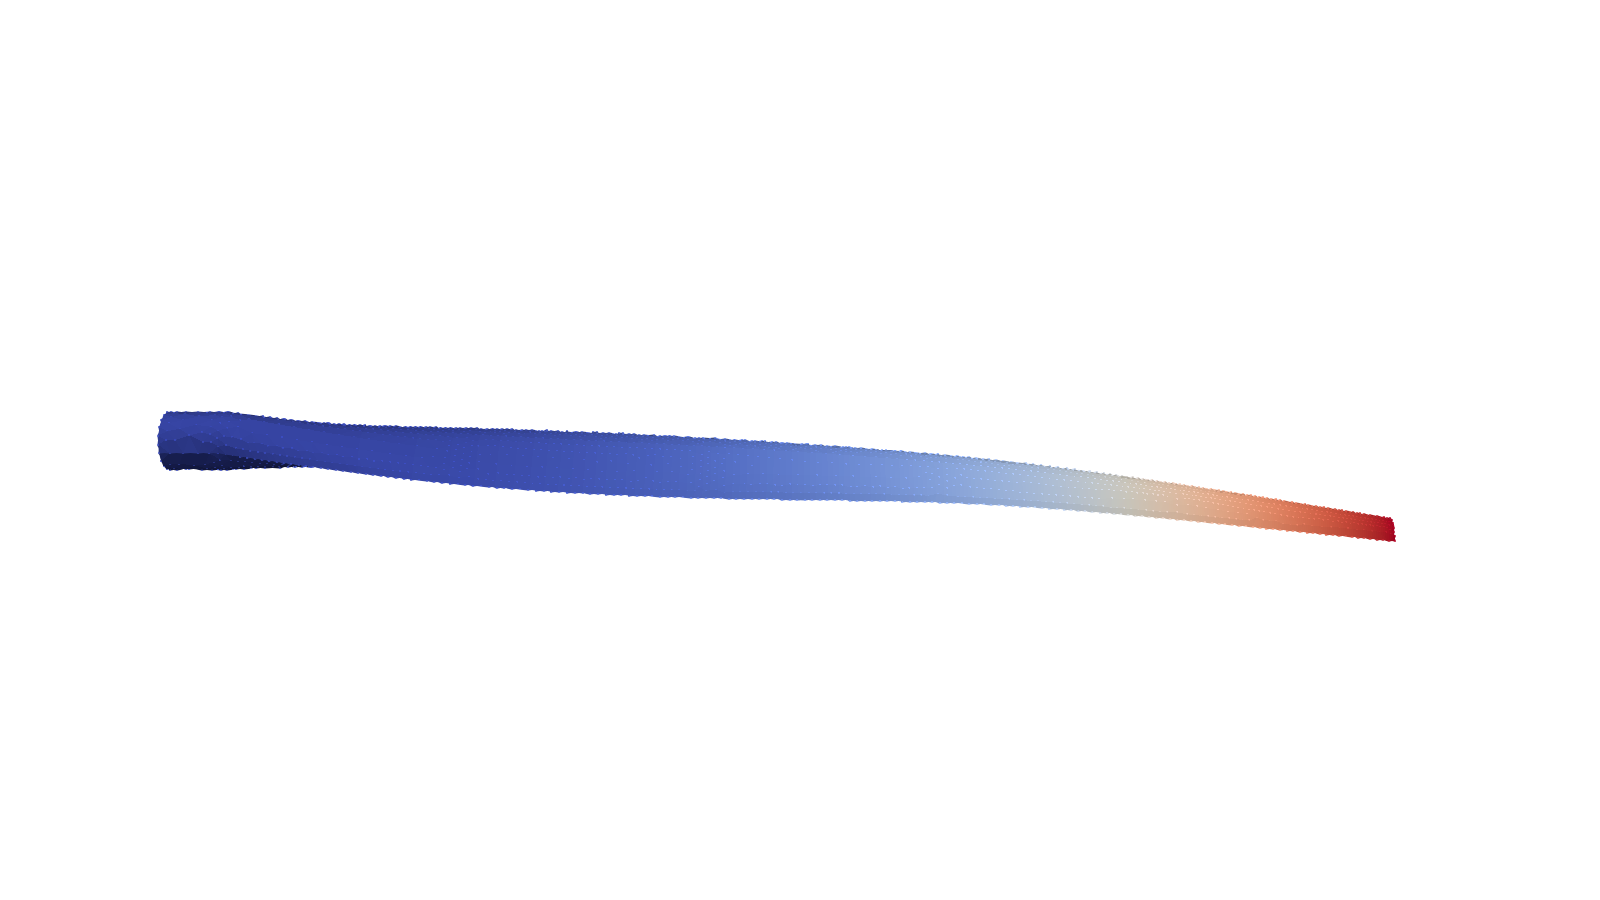
\includegraphics[width=\textwidth]{Figures/WindTurbineBladeModalAnalysisMode1.png}
        \caption{Mode 1: 0.81 Hz}
    \end{subfigure}
    \hfill
    \begin{subfigure}[b]{0.3\textwidth}
        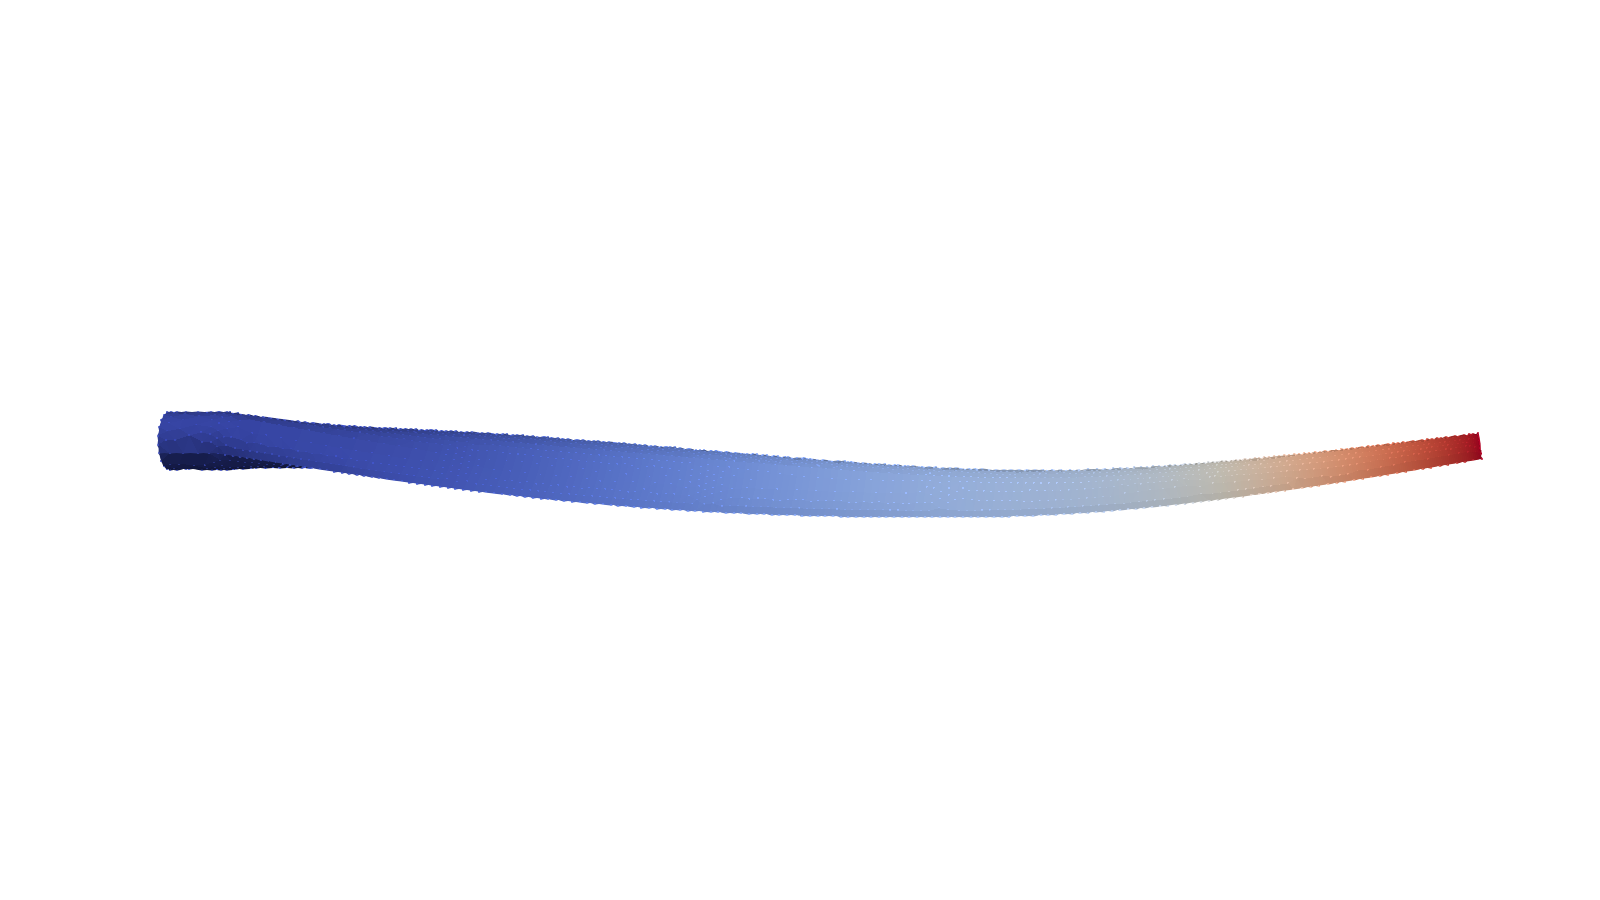
\includegraphics[width=\textwidth]{Figures/WindTurbineBladeModalAnalysisMode2.png}
        \caption{Mode 2: 1.90 Hz}
    \end{subfigure}
    \hfill
    \begin{subfigure}[b]{0.3\textwidth}
        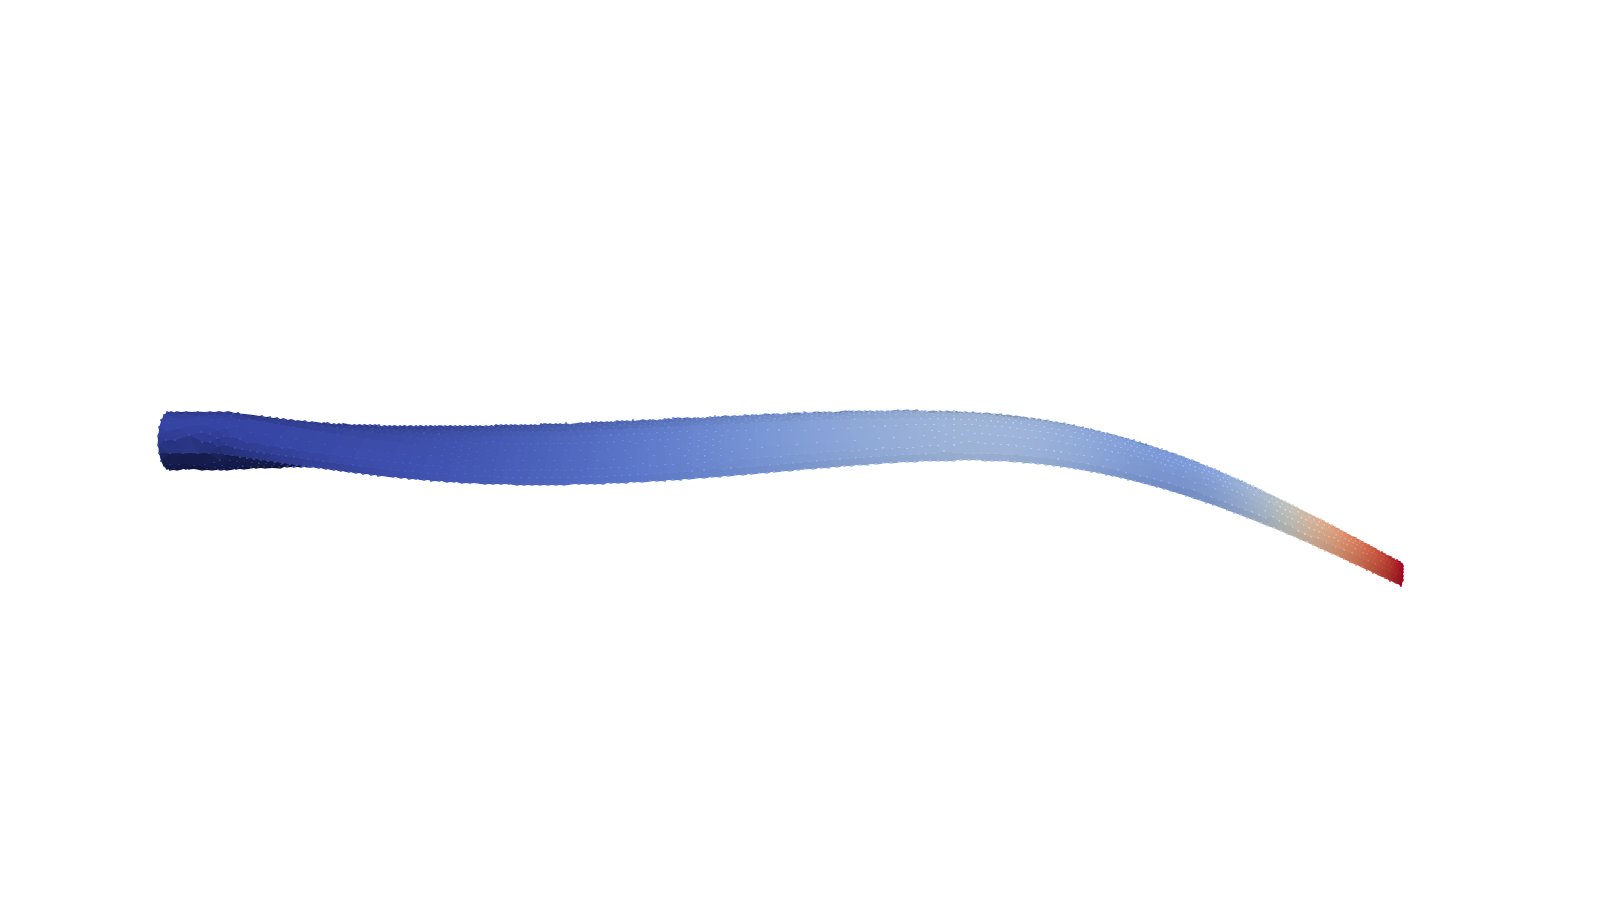
\includegraphics[width=\textwidth]{Figures/WindTurbineBladeModalAnalysisMode3.png}
        \caption{Mode 3: 2.51 Hz}
    \end{subfigure}
    
    \vspace{1em}
    
    \begin{subfigure}[b]{0.3\textwidth}
        
\includegraphics[width=\textwidth]{Figures/WindTurbineBladeModalAnalysisMode4.png}
        \caption{Mode 4: 5.37 Hz}
    \end{subfigure}
    \hfill
    \begin{subfigure}[b]{0.3\textwidth}
        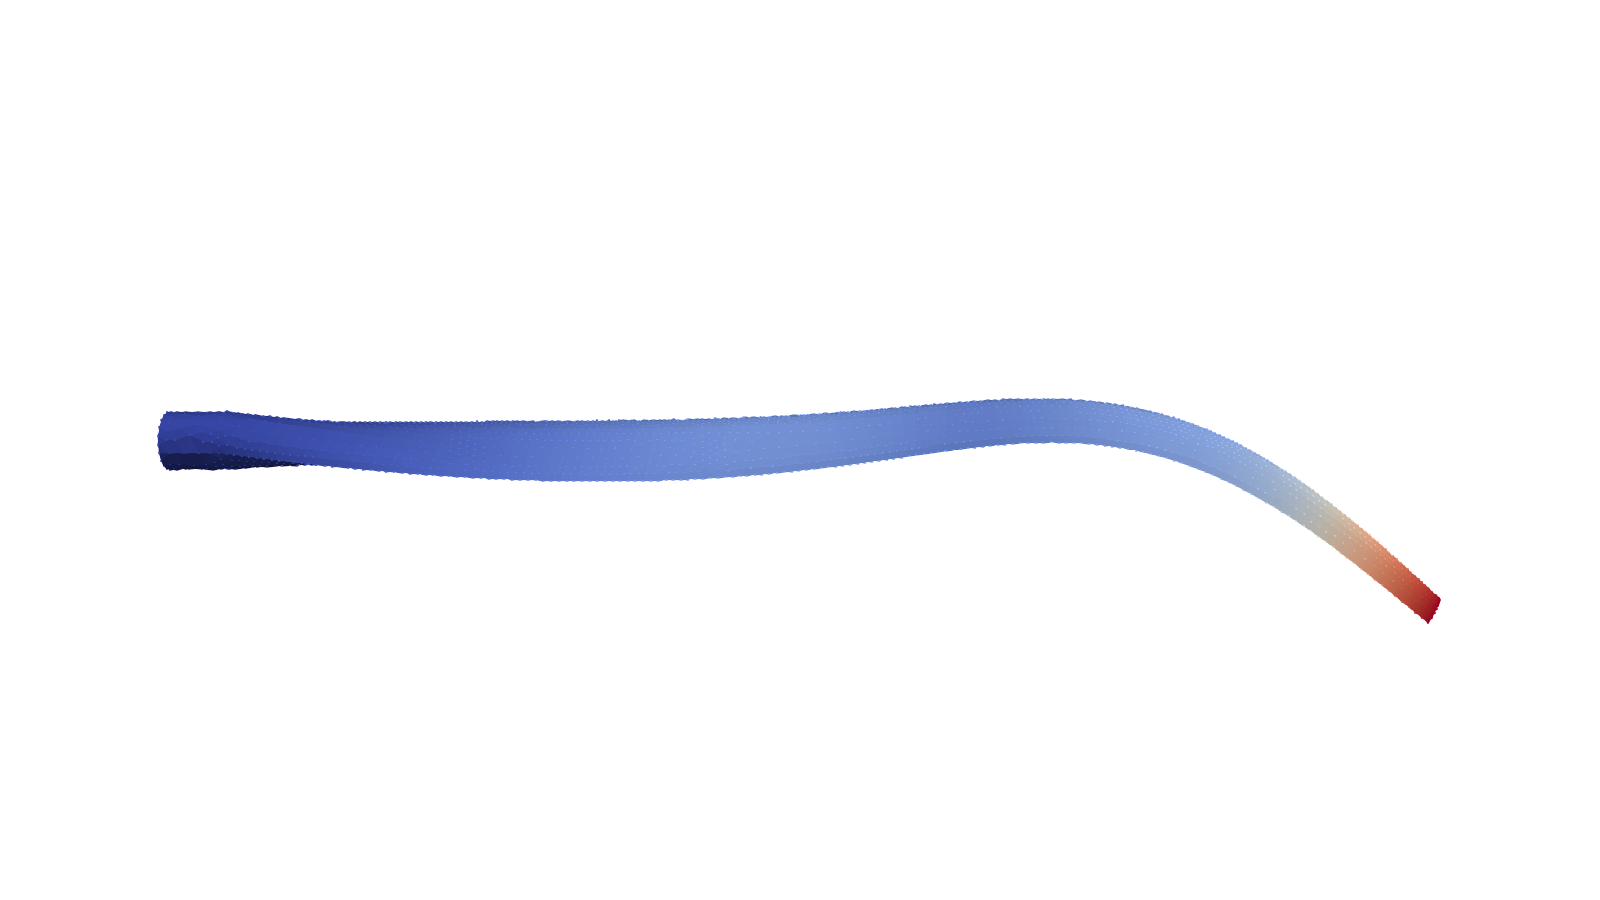
\includegraphics[width=\textwidth]{Figures/WindTurbineBladeModalAnalysisMode5.png}
        \caption{Mode 5: 6.21 Hz}
    \end{subfigure}
    \hfill
    \begin{subfigure}[b]{0.3\textwidth}
        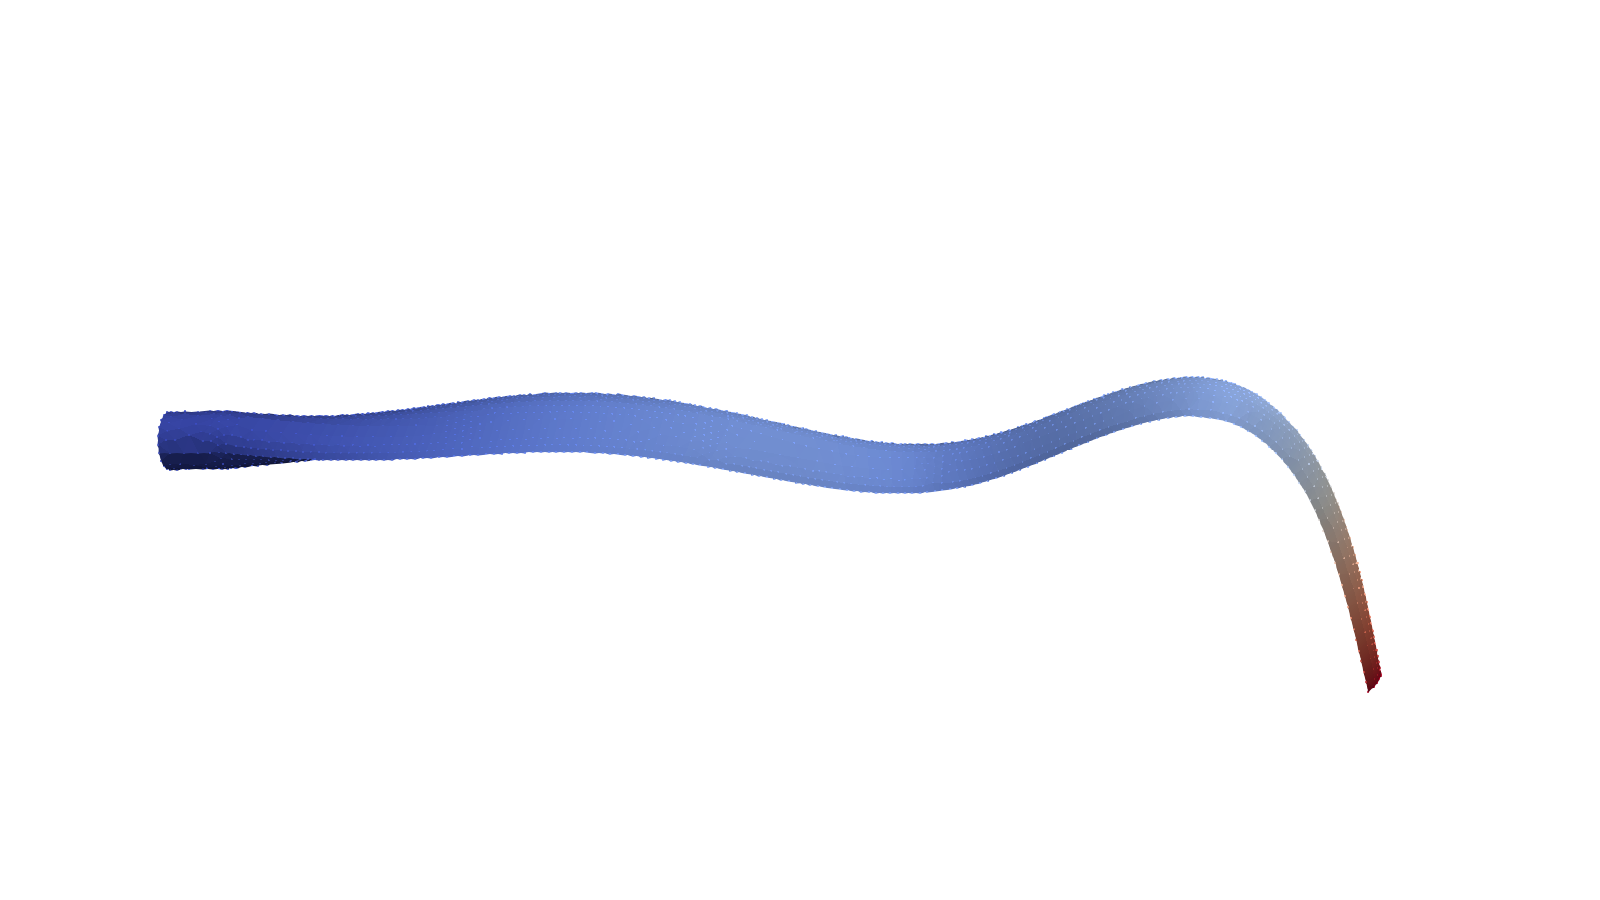
\includegraphics[width=\textwidth]{Figures/WindTurbineBladeModalAnalysisMode6.png}
        \caption{Mode 6: 9.41 Hz}
    \end{subfigure}

    \caption{
    First six vibration modes of the wind turbine blade obtained from free vibration analysis using linear elasticity. The modes are ordered by increasing natural frequency, ranging from 0.81 Hz to 9.41 Hz. The shapes reflect dominant deformation patterns, including bending and torsional behavior, and illustrate the concentration of dynamic energy in a small number of low-frequency modes.
    }
    \label{fig:blade_modes}
\end{figure}


Although the full-order model contains \( N = 17\,683 \) degrees of freedom, the blade's dynamic response is largely governed by a small number of low-frequency modes. This low-dimensional behavior supports the rationale behind projection-based reduction.

While modal analysis is not used directly in this thesis as a solver, it exemplifies the idea of restricting the dynamics to a low-dimensional subspace spanned by physically meaningful basis functions. It also motivates the need for more flexible, data-driven basis construction techniques, such as proper orthogonal decomposition, for problems where linearity, symmetry, or time-invariance do not hold.

\vspace{0.5em}
\textit{See, for example,}~\cite{craig2006fundamentals, meirovitch1975elements, kerschen2005method} \textit{for classical and modern treatments of modal analysis in structural dynamics.}

\section{Proper orthogonal decomposition}

Proper orthogonal decomposition (POD) constructs a low-dimensional linear subspace that best approximates a family of high-dimensional solution snapshots in the least-squares sense.  
Unlike classical modal analysis, POD is data-driven and makes no assumptions about linearity, symmetry, or time-invariance.

Let the system's behavior be governed by underlying equations (often partial differential equations) dependent on spatial coordinates $\mathbf{x} \in \Omega$, time $t \in [0, T]$, and a set of parameters $\boldsymbol{\mu} \in \mathcal{D} \subset \mathbb{R}^p$. The application of a suitable spatial discretization method (e.g., Finite Element, Finite Volume, Finite Difference) to these equations yields the high-fidelity solution, represented by a time- and parameter-dependent state vector $\mathbf{u} \in \mathbb{R}^N$, where $N$ is the number of degrees of freedom.

A specific instance of this discrete state vector at time $t$ and for parameter configuration $\boldsymbol{\mu}$ is denoted as:
\begin{equation}
\mathbf{u}(t, \boldsymbol{\mu}) \in \mathbb{R}^N
\end{equation}
This vector represents the high-dimensional state of the system within the chosen discretization.

For POD, solution snapshots are collected at selected discrete time instances $t_k \in \{t_1, t_2, \dots, t_{N_t}\} \subset [0, T]$ and for various parameter samples $\boldsymbol{\mu}_j \in \{\boldsymbol{\mu}_1, \boldsymbol{\mu}_2, \dots, \boldsymbol{\mu}_P\} \subset \mathcal{D}$. These snapshots are assembled into the columns of the snapshot matrix $\mathbf{S}$:

\begin{equation}
\label{eq:snapshot_matrix}
\mathbf{S} = 
\begin{bmatrix}
\mathbf{u}(t_1, \boldsymbol{\mu}_1), \mathbf{u}(t_2, \boldsymbol{\mu}_1), \dots, \mathbf{u}(t_{N_t}, \boldsymbol{\mu}_1), \mathbf{u}(t_1, \boldsymbol{\mu}_2), \dots, \mathbf{u}(t_{N_t}, \boldsymbol{\mu}_2), \dots, \mathbf{u}(t_1, \boldsymbol{\mu}_P), \dots, \mathbf{u}(t_{N_t}, \boldsymbol{\mu}_P)
\end{bmatrix}
\in \mathbb{R}^{N \times N_s},
\end{equation}
where $N_s = N_t \cdot P$ is the total number of snapshots or samples, $N_t$ is the number of time instances sampled per parameter, and $P$ is the number of parameter samples.

\paragraph{POD basis.}
Given the snapshot matrix $\mathbf{S} \in \mathbb{R}^{N \times N_s}$, the objective of POD is to find an orthonormal matrix $\boldsymbol{\Phi} \in \mathbb{R}^{N \times n}$, whose columns span the $n$-dimensional subspace that minimizes the Frobenius‐norm projection error:
\begin{equation}
\label{eq:pod_opt}
\min_{\boldsymbol{\Phi}^{\!T}\boldsymbol{\Phi}=\mathbf{I}_n}
\;\bigl\|\,\mathbf{S} - \boldsymbol{\Phi}\boldsymbol{\Phi}^{\!T}\mathbf{S}\bigr\|_{F}^{2}.
\end{equation}
Here, $\mathbf{I}_n$ is the $n \times n$ identity matrix, and $\boldsymbol{\Phi}\boldsymbol{\Phi}^{\!T}$ represents the orthogonal projector onto the subspace spanned by the columns of $\boldsymbol{\Phi}$. The solution to this optimization problem \eqref{eq:pod_opt} is obtained via the SVD of the snapshot matrix. Considering the thin SVD,
\begin{equation}
\mathbf{S}= \mathbf{U}\boldsymbol{\Sigma}\mathbf{V}^{\!T},
\end{equation}
where $\mathbf{U} \in \mathbb{R}^{N \times r}$ has orthonormal columns (left singular vectors), $\mathbf{V} \in \mathbb{R}^{N_s \times r}$ has orthonormal columns (right singular vectors), $r = \operatorname{rank}(\mathbf{S})$, and $\boldsymbol{\Sigma}=\operatorname{diag}(\sigma_1,\dots,\sigma_r) \in \mathbb{R}^{r \times r}$ contains the positive singular values ordered non-increasingly ($\sigma_1 \ge \sigma_2 \ge \dots \ge \sigma_r > 0$). The optimal rank-$n$ POD basis ($n \le r$) consists of the first $n$ left singular vectors:
\begin{equation}
\boldsymbol{\Phi}= \mathbf{U}_{[:,1:n]}.
\end{equation}

\paragraph{Energy criterion.}
A common heuristic for selecting the basis dimension $n$ involves monitoring the cumulative energy captured by the retained singular values. The \emph{squared POD energy loss}, or fraction of unexplained variance, is defined as:
\begin{equation}
\label{eq:pod_energy_loss}
\epsilon^{2}(n)
\;=\;
1 - \frac{\displaystyle\sum_{i=1}^{n}\sigma_i^{\,2}}
         {\displaystyle\sum_{j=1}^{r}\sigma_j^{\,2}},
\qquad 0 \le \epsilon^{2}(n) \le 1,
\end{equation}
This quantity $\epsilon^2(n)$ represents the fraction of energy discarded by the rank-$n$ approximation. Intuitively, it quantifies the proportion of the system’s dynamic energy not captured by the reduced basis.

It is equivalent to the squared relative reconstruction error of the snapshot matrix in the Frobenius norm:
\begin{equation}
\epsilon^2(n) = \frac{\|\mathbf{S} - \boldsymbol{\Phi}\boldsymbol{\Phi}^{\!T}\mathbf{S}\|_F^2}{\|\mathbf{S}\|_F^2}.
\end{equation}
Consequently, $\epsilon(n)$ is the relative Frobenius error associated with approximating $\mathbf{S}$ by its projection onto the $n$-dimensional POD basis $\boldsymbol{\Phi}$. A desired tolerance $\epsilon_{tol}$ is often set (e.g., $10^{-3}$), and the smallest $n$ is chosen such that $\epsilon(n) \le \epsilon_{tol}$.


\subsection{Projection-based reduced order model via Galerkin projection}

Let $\mathbf{R}(\mathbf{u}(t,\boldsymbol{\mu});\,t,\boldsymbol{\mu}) = \mathbf{0}$ 
denote a general discrete residual arising from a finite element, finite volume, or finite difference discretization, such as the one introduced in Section~\ref{sec:model_problem}. 
Here, $\mathbf{u}(t,\boldsymbol{\mu}) \in \mathbb{R}^N$ is the full-order solution at time $t$ and parameter $\boldsymbol{\mu} \in \mathcal{D}$.

In projection-based model reduction, $\mathbf{u}(t,\boldsymbol{\mu})$ is approximated as
\begin{equation}
\mathbf{u}(t,\boldsymbol{\mu}) \;\approx\; 
\mathbf{\tilde{u}}(t,\boldsymbol{\mu}) 
= \mathbf{u}_{\text{ref}} + \boldsymbol{\Phi}\,\mathbf{q}(t,\boldsymbol{\mu}),
\end{equation}
where $\mathbf{u}_{\text{ref}} \in \mathbb{R}^N$ is a reference state, 
$\boldsymbol{\Phi} \in \mathbb{R}^{N \times n}$ is the reduced basis matrix, 
and $\mathbf{q}(t,\boldsymbol{\mu}) \in \mathbb{R}^n$ are the reduced generalized coordinates. 
The reference $\mathbf{u}_{\text{ref}}$ is often chosen as the mean of the snapshot set or as the initial condition of the system. 
For simplicity, and without loss of generality in the following derivations, 
we take $\mathbf{u}_{\text{ref}} = \mathbf{0}$.  

The encoder–decoder structure of this approximation is illustrated in Figure~\ref{fig:linear_reduction_encoder_decoder}.


\begin{figure}[ht!]
    \centering
    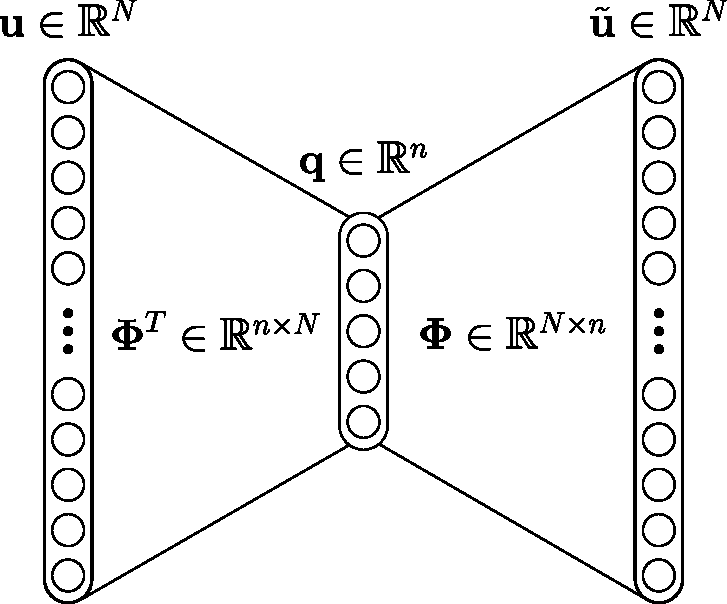
\includegraphics[width=0.5\textwidth]{Figures/linear_prom_encoder_decoder.pdf}
    \caption{
    Schematic representation of the linear subspace reduction and reconstruction process.
    The high-dimensional state \( \mathbf{u} \in \mathbb{R}^N \) is projected onto a low-dimensional subspace via \( \mathbf{q} = \boldsymbol{\Phi}^T \mathbf{u} \), and an approximation \( \tilde{\mathbf{u}} = \boldsymbol{\Phi} \mathbf{q} \) is reconstructed from the reduced coordinates \( \mathbf{q} \in \mathbb{R}^n \).
    }
    \label{fig:linear_reduction_encoder_decoder}
\end{figure}


The Galerkin projection seeks a reduced solution such that the residual is orthogonal to the subspace spanned by \( \boldsymbol{\Phi} \), i.e.,
\begin{equation}
\boldsymbol{\Phi}^{\!T}\,\mathbf{R}\bigl(\boldsymbol{\Phi}\,\mathbf{q}(t,\boldsymbol{\mu});\, t,\boldsymbol{\mu}\bigr) = \mathbf{0},
\label{eq:galerkin_orthogonality}
\end{equation}

\begin{equation}
\mathbf{R}_{r}\bigl(\mathbf{q}(t,\boldsymbol{\mu});\, t,\boldsymbol{\mu}\bigr)
\;:=\;
\boldsymbol{\Phi}^{\!T}\,\mathbf{R}\bigl(\boldsymbol{\Phi}\,\mathbf{q}(t,\boldsymbol{\mu});\, t,\boldsymbol{\mu}\bigr)
\in \mathbb{R}^{n}.
\label{eq:galerkin_reduced_residual}
\end{equation}



In the nonlinear case, the reduced system cannot be solved directly and requires iterative methods. A common approach is Newton’s method (applied to the projected residual), which yields the reduced linear system at each iteration (schematically illustrated in Figure~\ref{fig:galerkin_newton_projection}):
\begin{subequations}
\begin{align}
\mathbf{J}_{r}\bigl(\mathbf{q}^{(k)}(t,\boldsymbol{\mu});\,t,\boldsymbol{\mu}\bigr)\,\delta \mathbf{q}^{(k)} 
&= -\,\mathbf{R}_{r}\bigl(\mathbf{q}^{(k)}(t,\boldsymbol{\mu});\,t,\boldsymbol{\mu}\bigr),
\label{eq:galerkin_newton_linear}\\[0.5em]
\mathbf{q}^{(k+1)}(t,\boldsymbol{\mu}) 
&= \mathbf{q}^{(k)}(t,\boldsymbol{\mu}) + \delta \mathbf{q}^{(k)}.
\label{eq:galerkin_newton_update}
\end{align}
\end{subequations}


\begin{figure}[ht!]
    \centering
    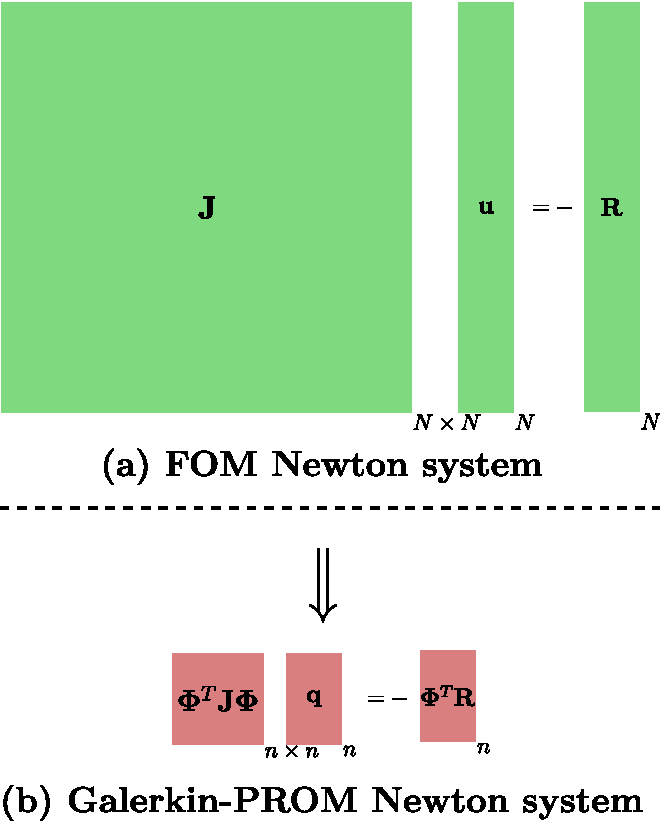
\includegraphics[width=0.52\textwidth]{Figures/SystemReduction2.pdf}
    \caption{
    Visual comparison of Newton systems before and after Galerkin projection.
    \textbf{(a)} Full-order model (FOM) Newton system: the nonlinear system is defined over the high-dimensional space \( \mathbb{R}^N \), involving the full residual \( \mathbf{R} \) and Jacobian \( \mathbf{J} \).
    \textbf{(b)} Galerkin-PROM system: projection via the reduced basis \( \boldsymbol{\Phi} \) yields a low-dimensional system in terms of reduced coordinates \( \mathbf{q} \in \mathbb{R}^n \).
    }
    \label{fig:galerkin_newton_projection}
\end{figure}


where \( \delta \mathbf{q} \in \mathbb{R}^n \) is the correction to the reduced state iterate, and the reduced Jacobian \( \mathbf{J}_{r} \) (evaluated at the current iterate \( \mathbf{q}(t, \boldsymbol{\mu}) \)) is given by
\begin{equation}
\label{eq:reduced_jacobian}
\mathbf{J}_{r}\bigl(\mathbf{q}(t,\boldsymbol{\mu});\,t,\boldsymbol{\mu}\bigr) 
= \boldsymbol{\Phi}^{\!T}\,
\mathbf{J}\bigl(\boldsymbol{\Phi}\,\mathbf{q}(t,\boldsymbol{\mu});\,t,\boldsymbol{\mu}\bigr)\,
\boldsymbol{\Phi}
\;\in\; \mathbb{R}^{n \times n}.
\end{equation}
Here, \( \mathbf{J}(\mathbf{u};\,t,\boldsymbol{\mu}) \in \mathbb{R}^{N \times N} \) is the full-order Jacobian matrix, defined as the derivative of the full-order residual with respect to the full-order state:
\begin{equation}
\label{eq:full_jacobian_def}
\mathbf{J}\bigl(\mathbf{u}(t,\boldsymbol{\mu});\,t,\boldsymbol{\mu}\bigr) 
:= \frac{\partial \mathbf{R}\bigl(\mathbf{u}(t,\boldsymbol{\mu});\,t,\boldsymbol{\mu}\bigr)}{\partial \mathbf{u}}.
\end{equation}

In Equation~\eqref{eq:reduced_jacobian}, the full-order Jacobian \( \mathbf{J} \) is evaluated at the state corresponding to the current reduced iterate, i.e., \( \mathbf{u}(t, \boldsymbol{\mu}) = \boldsymbol{\Phi}\mathbf{q}(t, \boldsymbol{\mu}) \).

While Galerkin projection is optimal when the full-order Jacobian 
\(\mathbf{J}\bigl(\mathbf{u}(t,\boldsymbol{\mu});\,t,\boldsymbol{\mu}\bigr)\) 
is symmetric and positive-definite, it may perform poorly for convection-dominated problems, as there is no guarantee of optimality. A more general treatment of these issues is provided in Section~\ref{subsec:galerkin_lspg_comparison} and Chapter~\ref{chap:article1}, where a Petrov--Galerkin formulation is introduced.

\subsection{POD-Galerkin PROM for the wind turbine blade}

To demonstrate the capabilities of POD for nonlinear dynamics and overcome the limitations of linear modal analysis, a projection-based reduced-order model is developed for the turbine blade. This problem, governed by second-order structural dynamics, is representative of a \emph{parabolic-type} system, characterized by smooth time evolution and symmetric positive-definite operators. The PROM is constructed using snapshots generated by a high-fidelity simulation (FOM).

\paragraph{Full-order model.}
The geometry, illustrated in Figure~\ref{fig:blade_geometry}, corresponds to a utility-scale wind turbine blade approximately 43.2~m in length, with a maximum chord of 3.1~m and a root diameter of around 2~m. The structure is modeled as a solid, homogeneous, and isotropic body to simplify internal detail while retaining global flexibility. The material properties are defined as
\begin{equation}
\rho = 108.48\;\text{kg\,m}^{-3}, 
\qquad   
E   = 2.333\;\text{GPa},
\qquad   
\nu = 0.29.
\end{equation}
The structural response is computed via dynamic analysis using Total Lagrangian solid elements and a compressible Neo-Hookean hyperelastic constitutive law. Large displacements and geometric nonlinearity are fully accounted for. The blade is clamped at the root by homogeneous Dirichlet conditions, no damping is included, and time integration is performed using the implicit Newmark average-acceleration method. The resulting FOM comprises $13\,488$ elements and $17\,683$ degrees of freedom.

\begin{figure}[ht!]
    \centering
    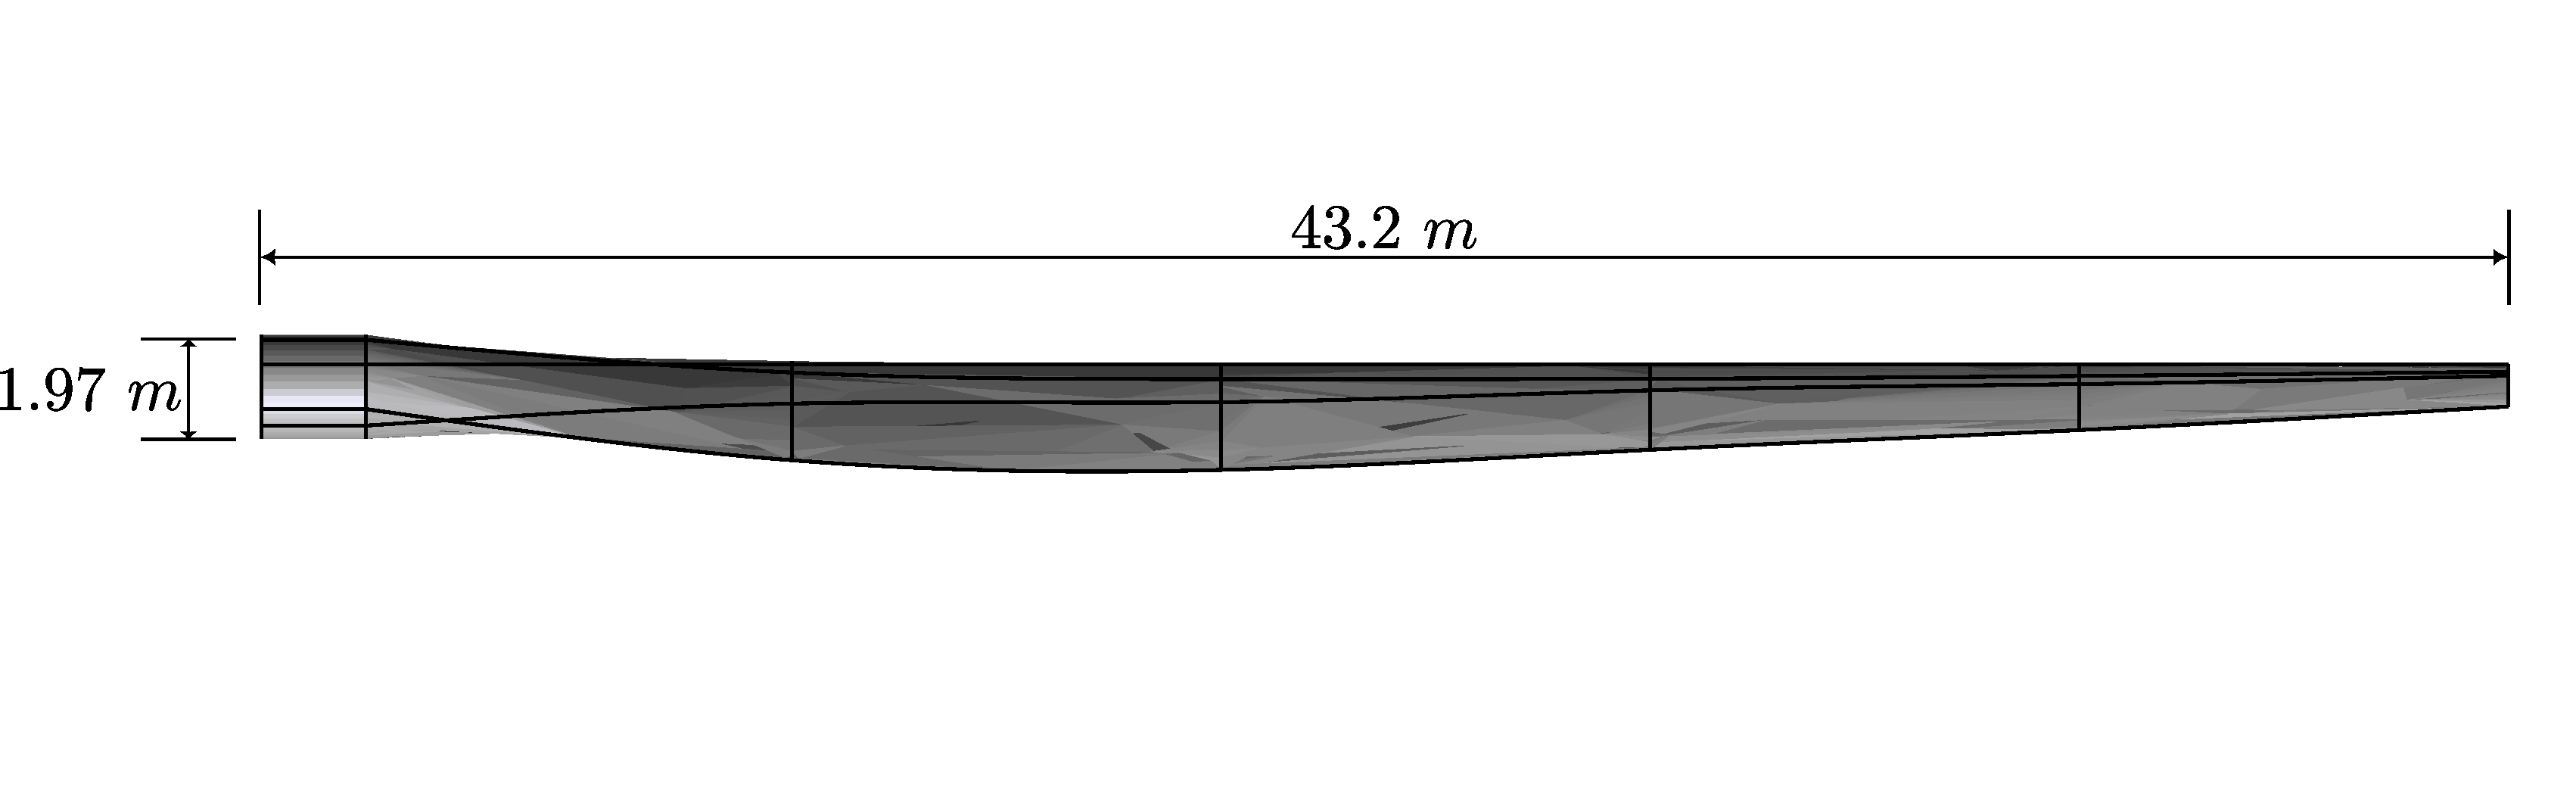
\includegraphics[width=0.85\textwidth]{Figures/WindTurbineBladeGeometry.pdf}
    \caption{
        Geometry and dimensions of the blade under study.
    }
    \label{fig:blade_geometry}
\end{figure}



\paragraph{Transient surface loading.}
Four smooth pressure pulses are imposed on the suction side, each lasting \(T_p = 2\,\text{s}\).  
The spatial and temporal variation is defined as
\begin{equation}
f(x,t) = A_i\, \sin^2\left( \dfrac{\pi (t - t_i)}{T_p} \right) \left( \frac{x}{L} \right)^2, \qquad t \in [t_i, t_i + T_p],
\end{equation}
where \(x\) denotes the axial position along the blade length. The amplitudes are specified as \(A = [500, 400, 600, 300]\,\text{Pa}\) for the training case and \(A = [500, 350, 650, 250]\,\text{Pa}\) for testing.

\begin{figure}[ht!]
    \centering
    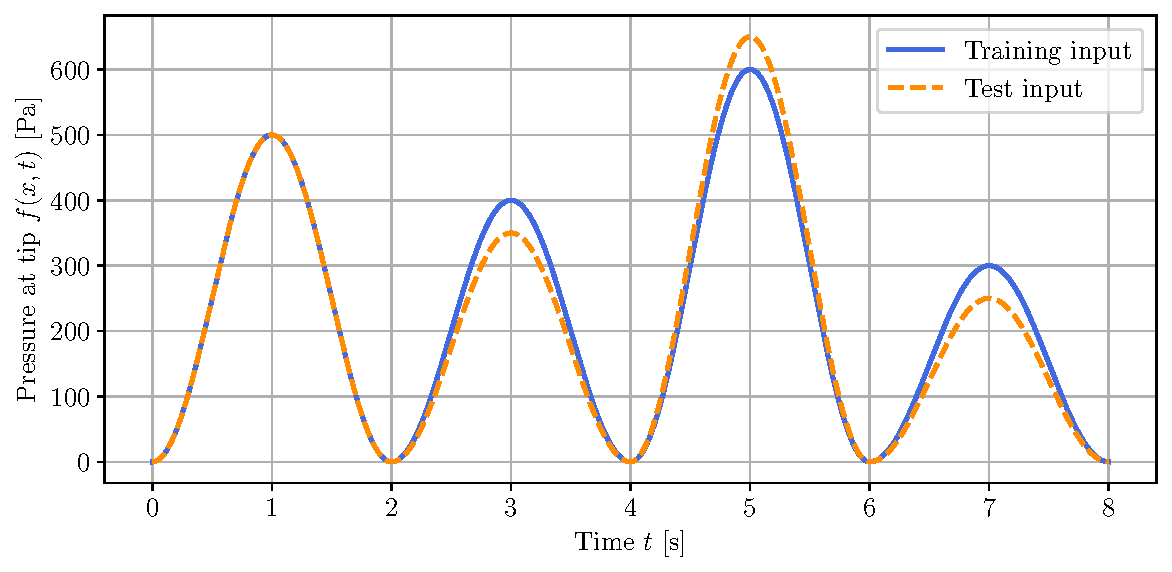
\includegraphics[width=0.85\textwidth]{Figures/training_vs_test_pressure_tip_pa.pdf}
    \caption{
        Time evolution of the pressure input at the blade tip for both training and test cases. 
        Each case consists of four localized pulses with smooth temporal profiles and slight amplitude variations used to evaluate generalization.
    }
    \label{fig:training_test_pulses}
\end{figure}

These loads drive the blade tip through displacements of approximately \(4\,\text{m}\), which is sufficient to trigger pronounced nonlinear effects while remaining within physically plausible bounds for large-scale blades (see Figure~\ref{fig:training_test_pulses}).


\paragraph{Snapshot collection and POD.}
The simulation is performed over a time interval \(t \in [0, 8]\,\text{s}\), using a constant time step \(\Delta t = 0.01\,\text{s}\). A total of 800 solution snapshots are collected during the training run and arranged into the snapshot matrix \(\mathbf{S} \in \mathbb{R}^{N \times N_s}\), where each column corresponds to a full-order solution vector at a given time.  
The singular values of \(\mathbf{S}\) decay rapidly (Figure~\ref{fig:svd_decay}), and the first \(n\) modes capture nearly all of the dynamic energy, enabling an efficient low-rank representation of the system evolution.

\begin{figure}[ht!]
    \centering
    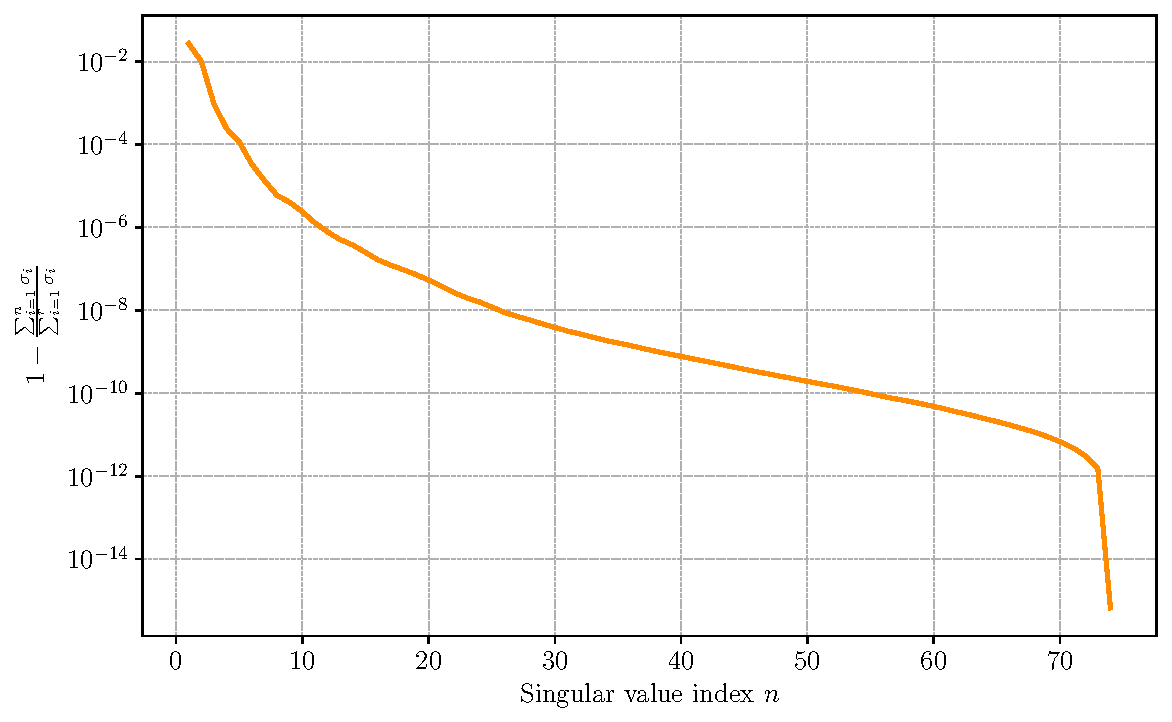
\includegraphics[width=0.65\textwidth]{Figures/svd_relative_loss_linear.pdf}
    \caption{
    Decay of the singular value energy fraction of the singular values of the snapshot matrix. The rapid decay reflects the compressibility of the solution manifold and justifies the use of a low-rank approximation.
    }
    \label{fig:svd_decay}
\end{figure}



\paragraph{POD basis and PROM assembly.}
The leading POD modes (Figure~\ref{fig:blade_pod_modes}) furnish the trial basis \(\boldsymbol{\Phi}\).  
Galerkin projection of the discrete residual yields the POD PROM.  
Accuracy is assessed against the perturbed test pulses.

\begin{figure}[ht!]
    \centering
    \begin{subfigure}[b]{0.3\textwidth}
        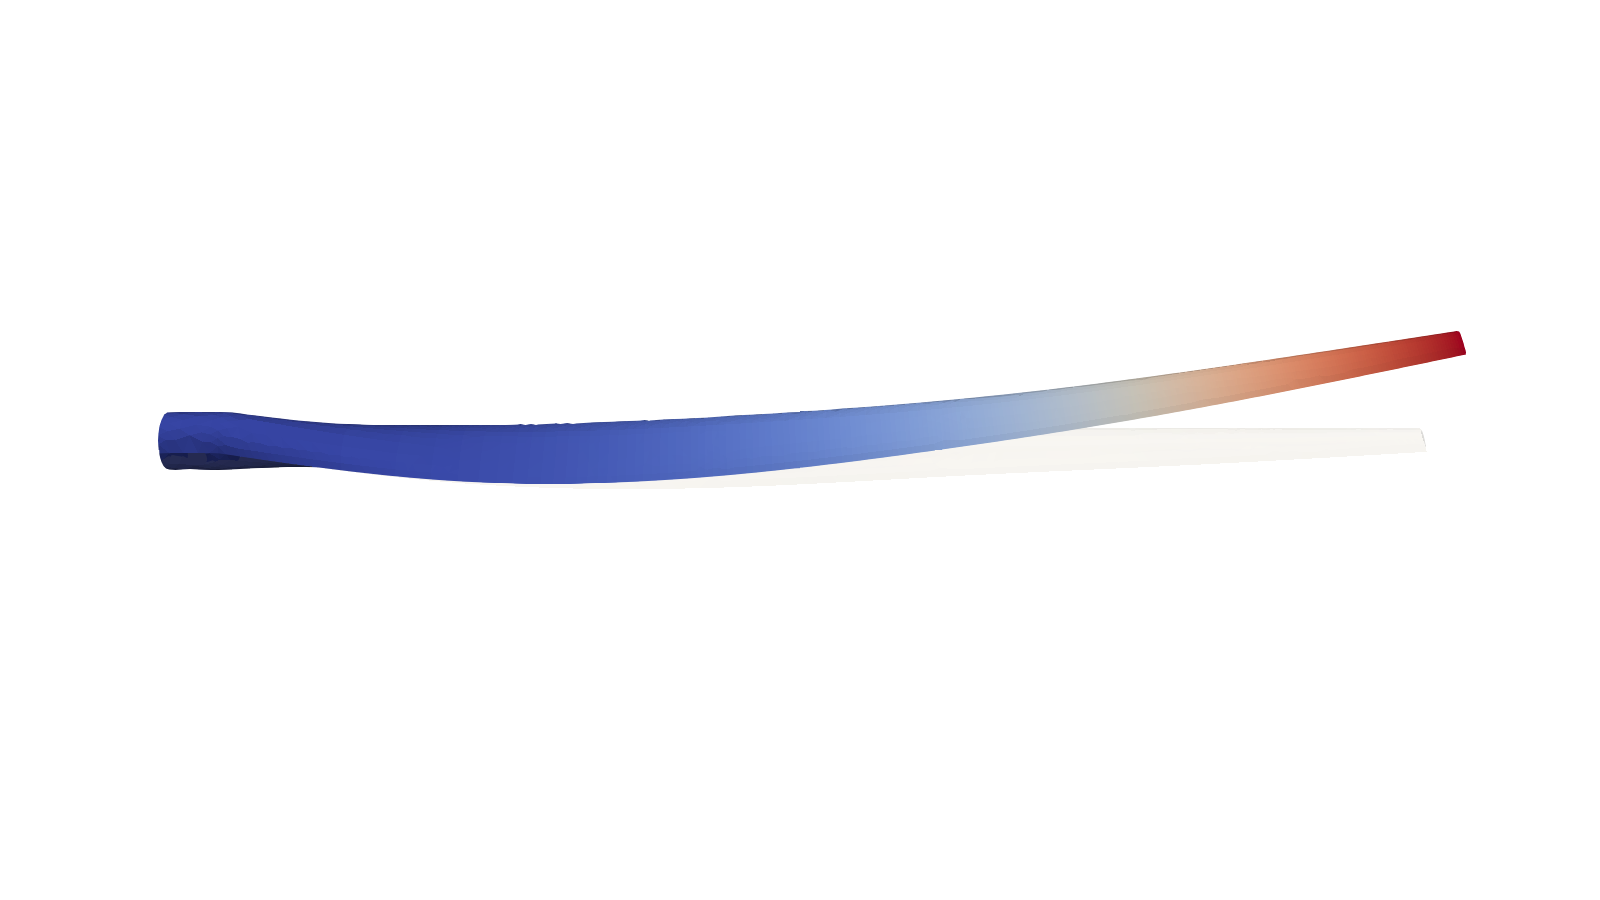
\includegraphics[width=\textwidth]{Figures/WindTurbineBladePODMode1.png}
        \caption{Mode 1}
    \end{subfigure}
    \hfill
    \begin{subfigure}[b]{0.3\textwidth}
        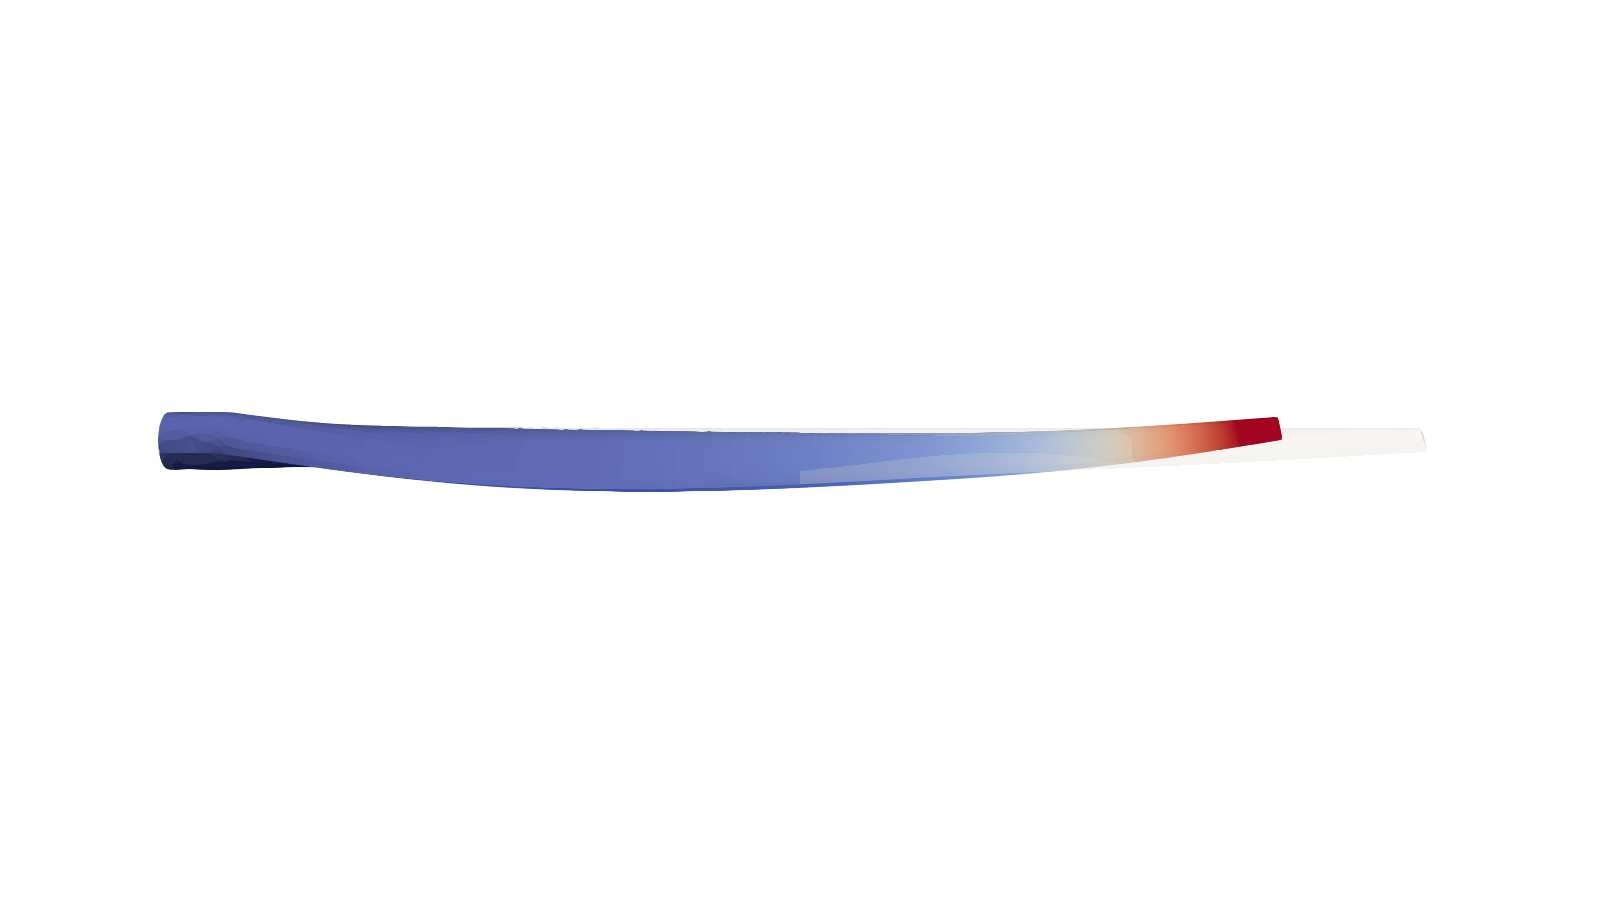
\includegraphics[width=\textwidth]{Figures/WindTurbineBladePODMode2.png}
        \caption{Mode 2}
    \end{subfigure}
    \hfill
    \begin{subfigure}[b]{0.3\textwidth}
        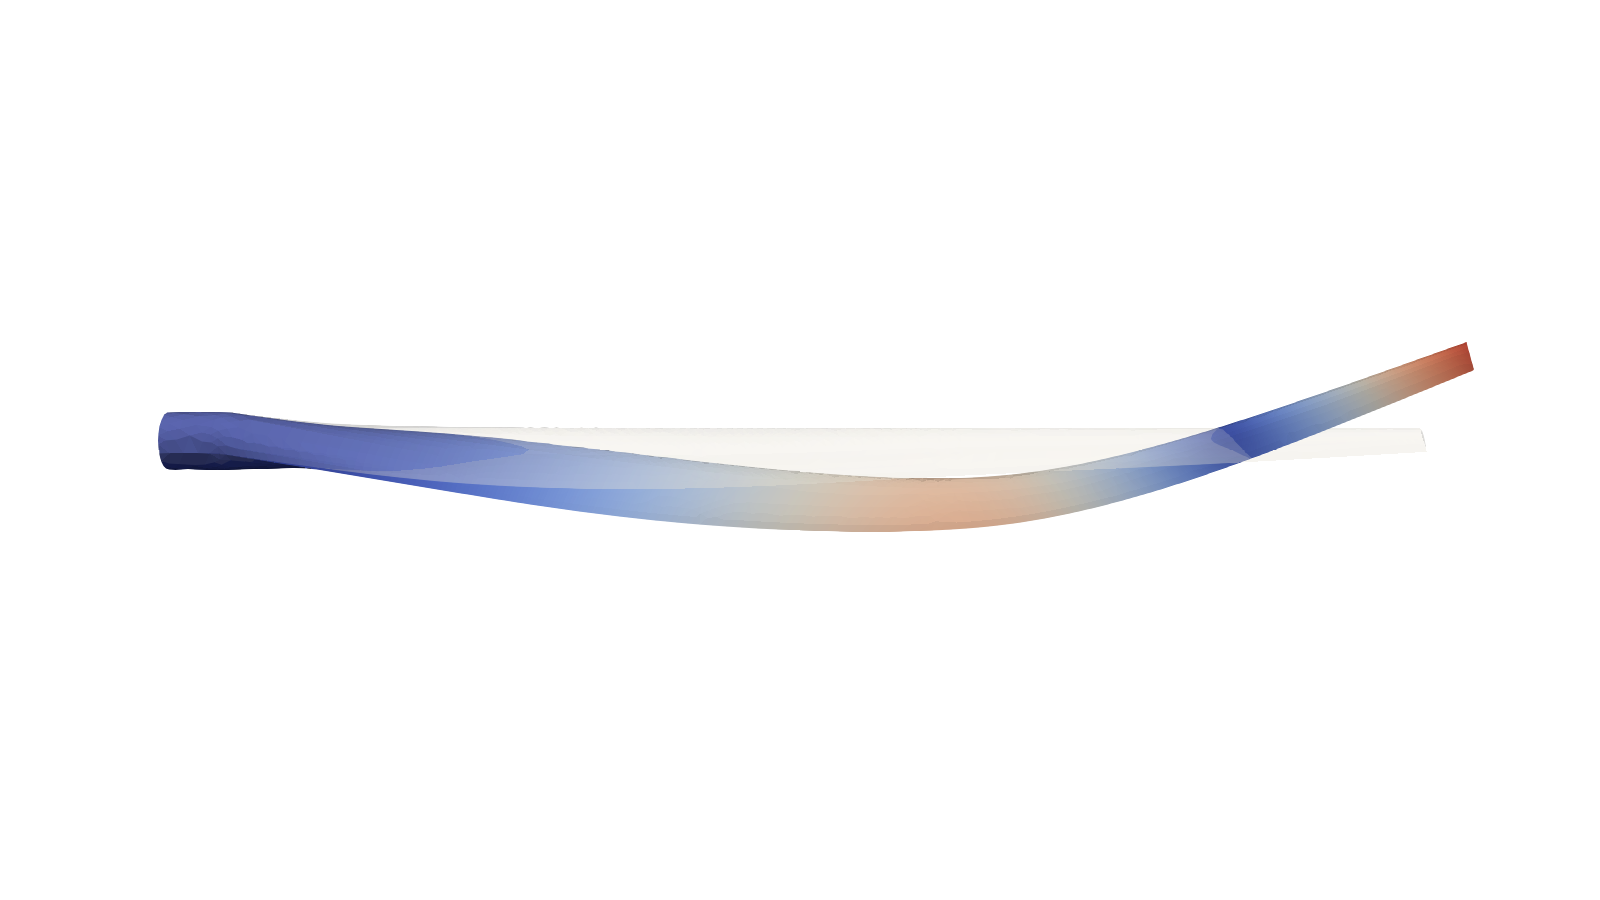
\includegraphics[width=\textwidth]{Figures/WindTurbineBladePODMode3.png}
        \caption{Mode 3}
    \end{subfigure}
    
    \vspace{1em}
    
    \begin{subfigure}[b]{0.3\textwidth}
        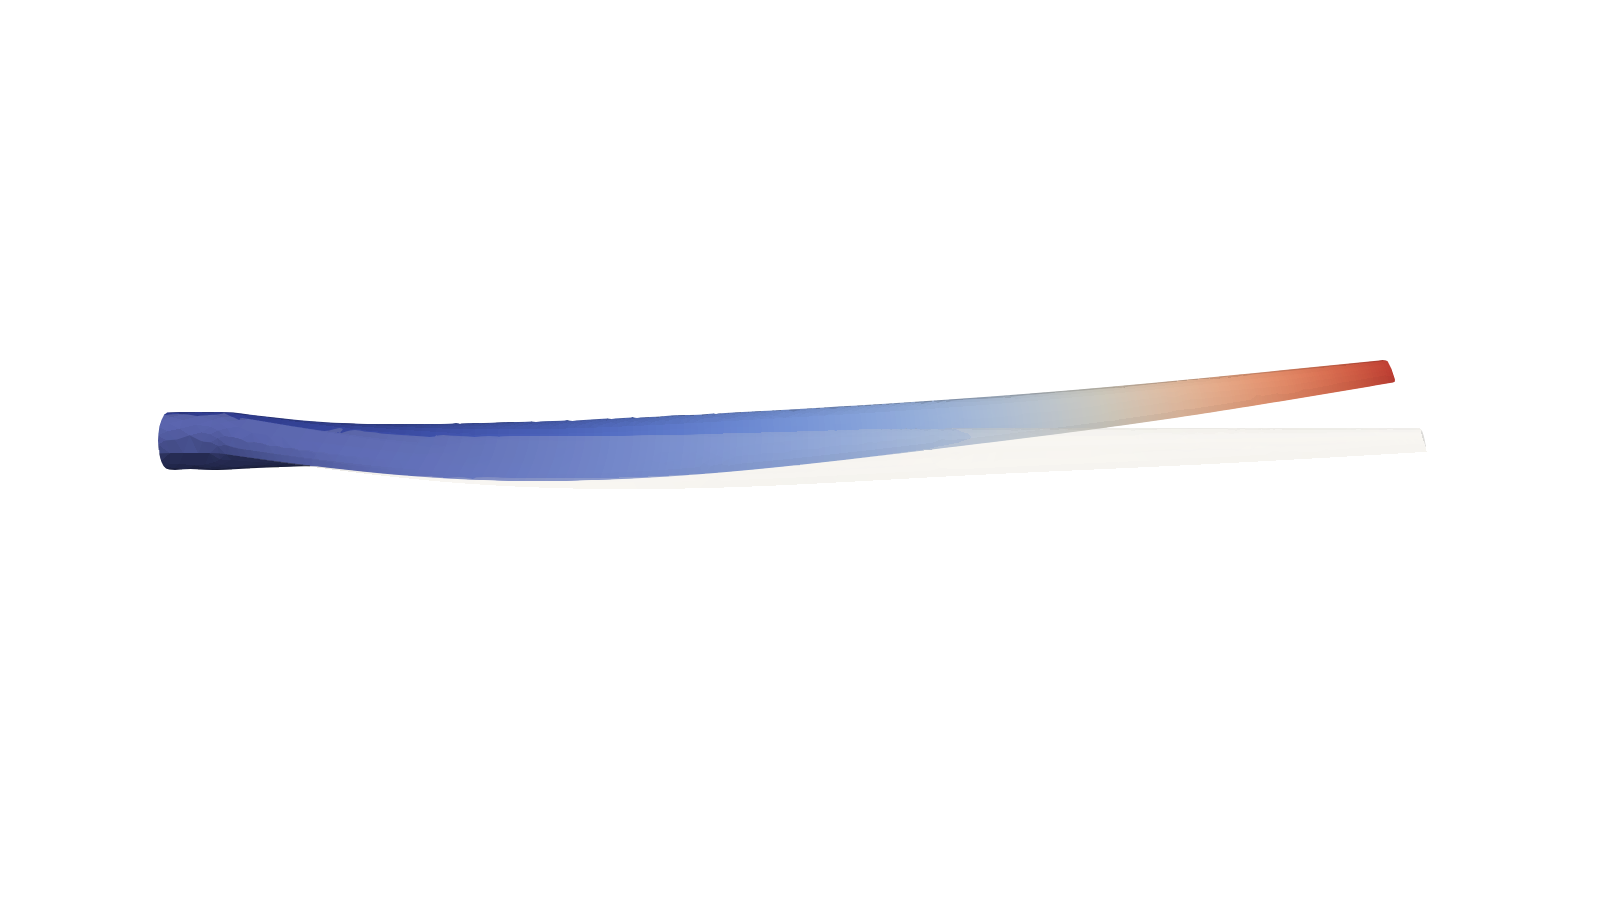
\includegraphics[width=\textwidth]{Figures/WindTurbineBladePODMode4.png}
        \caption{Mode 4}
    \end{subfigure}
    \hfill
    \begin{subfigure}[b]{0.3\textwidth}
        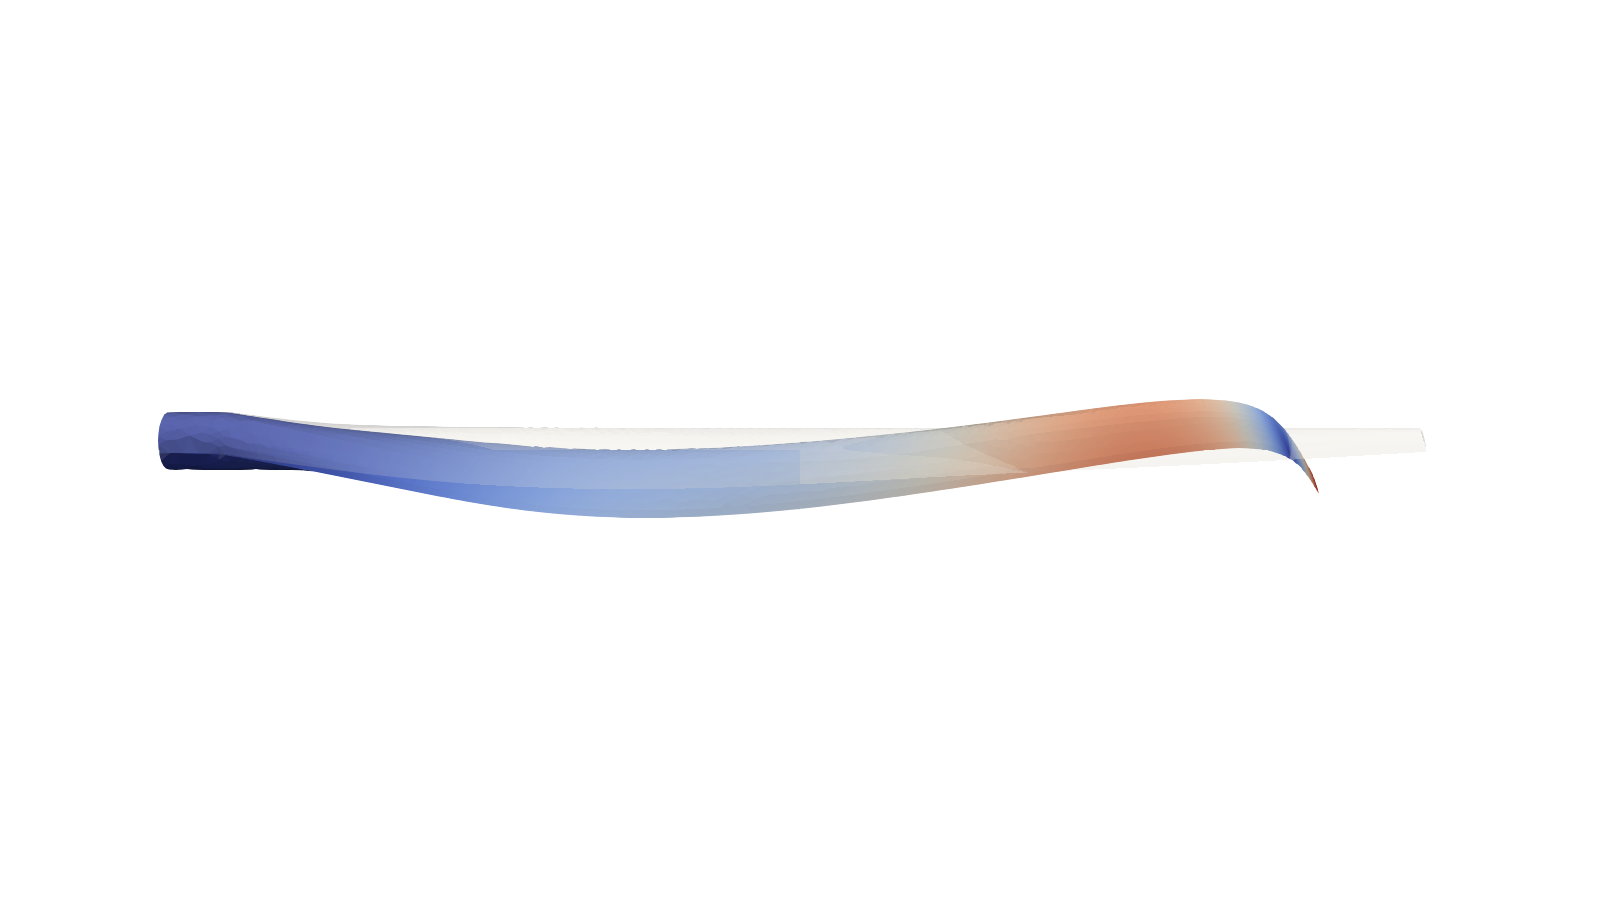
\includegraphics[width=\textwidth]{Figures/WindTurbineBladePODMode5.png}
        \caption{Mode 5}
    \end{subfigure}
    \hfill
    \begin{subfigure}[b]{0.3\textwidth}
        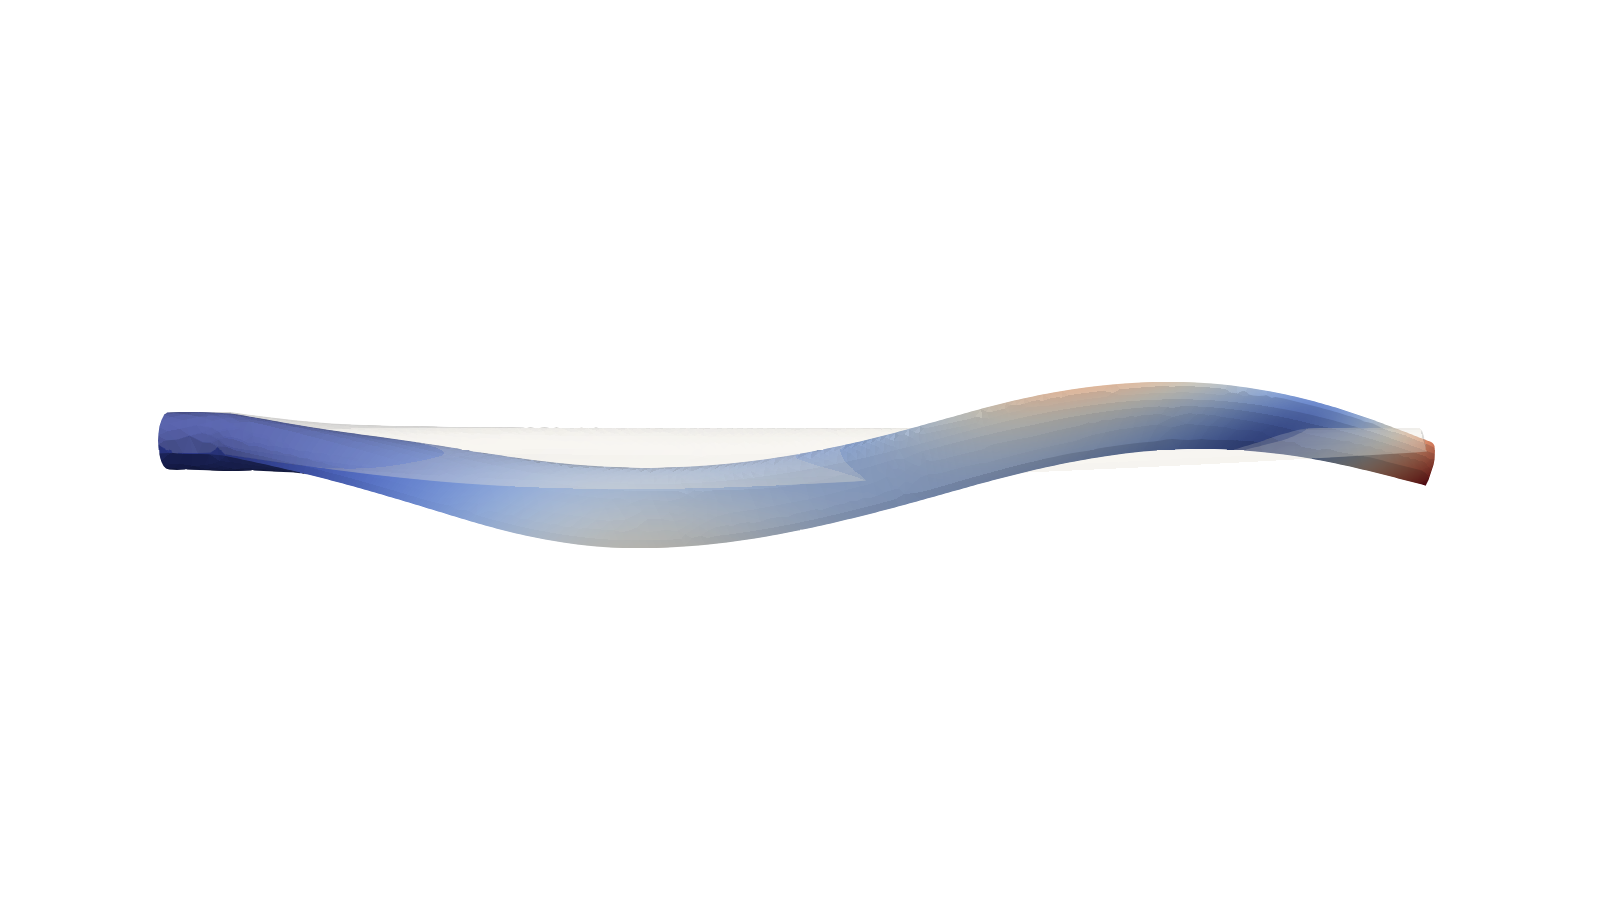
\includegraphics[width=\textwidth]{Figures/WindTurbineBladePODMode6.png}
        \caption{Mode 6}
    \end{subfigure}

    \caption{
    First six POD modes extracted from the full-order dynamic response of the wind turbine blade. These data-driven modes reflect dominant spatial deformation patterns learned from the high-fidelity simulation and serve as an efficient reduced basis for model order reduction.
    }
    \label{fig:blade_pod_modes}
\end{figure}


\paragraph{Results.}
A POD-based PROM is constructed using \(n=7\) modes based on maintaining a squared energy loss below \(\epsilon^2(n) \le 10^{-10}\). This criterion corresponds to a snapshot reconstruction error of \(\epsilon(n) = 10^{-5}\). 
When evaluated against the unseen test case loading, this 7-mode PROM achieves good predictive accuracy, exhibiting a relative error of approximately 0.14\% compared to the FOM. 
This relative error, denoted \(\mathbb{RE}_{2,\mathbf{u}}\), quantifies the difference between the PROM (\(\mathbf{\tilde{u}}\)) and FOM (\(\mathbf{u}\)) solutions over the trajectory for the test parameter case \(\boldsymbol{\mu}_{\text{test}}\), calculated using the time-accumulated 2-norm as:
\begin{equation} \label{eq:relative_error_def}
\mathbb{RE}_{2,\mathbf{u}} = 100\times\frac{\sqrt{\sum_{m=0}^{N_t} \|\mathbf{u}(t_m, \boldsymbol{\mu}_{\text{test}}) - \mathbf{\tilde{u}}(t_m, \boldsymbol{\mu}_{\text{test}})\|_2}}{\sqrt{\sum_{m=0}^{N_t} \|\mathbf{u}(t_m, \boldsymbol{\mu}_{\text{test}})\|_2}}.
\end{equation}
Qualitative comparisons of the tip displacement time histories and spatial deformation patterns are presented in Figure~\ref{fig:fom_vs_rom_tip} and Figure~\ref{fig:fom_rom_snapshots}, respectively.

Key quantitative performance metrics are summarised in Table~\ref{tab:rom_hrom_performance}. 
In terms of computational cost, the total wall-clock time was reduced from $348.41\,\text{s}$ for the FOM to $190.48\,\text{s}$ for the ROM, yielding an overall speed-up factor of $1.83\times$. 
This speed-up, while beneficial, is modest compared to the potential suggested by the drastic reduction in degrees of freedom ($N/n \approx 2526\times$). 
The discrepancy arises because, while the time required to solve the linear System of Equations (SoE) arising at each time step (or nonlinear iteration) is reduced dramatically (from \(0.20\,\text{s}\) for the FOM to \(8.3 \times 10^{-6}\,\text{s}\) for the ROM, yielding a speed-up factor of \(24\,096\times\)), the cost of assembling the reduced residual and Jacobian vectors dominates the computation. 
In the standard Galerkin projection framework used here, this assembly requires evaluating nonlinear terms over the full mesh ($13\,488$ elements), making its cost dependent on the FOM size. 
Therefore, despite the significant reduction in degrees of freedom, the computational complexity remains tied to the original FOM size. Addressing this assembly bottleneck is crucial for achieving substantial wall-clock time reductions and motivates the use of hyper-reduction techniques, which are introduced in the following section.

\subsection{Achieving real-time performance via hyper-reduction}
\label{sec:hrom_summary}

Despite the reduction in degrees of freedom achieved by the POD--Galerkin model (\(n = 7 \ll N = 17\,683\)), the total computational cost remains significantly influenced by the full-order discretization. This is because the residual and Jacobian assembly in the finite-element setting requires looping over all \(N_e = 13{,}488\) elements, with each elemental contribution accumulated into the global system.

Hyper-reduction techniques address this bottleneck by approximating the residual projection using only a subset of elements.  
Consider the full-order residual, assembled element-by-element,
\begin{equation}
\mathbf{R}(\boldsymbol{\Phi}\,\mathbf{q}) 
= \sum_{e=1}^{N_e} 
    \mathbf{L}_{e}^{\!T}\,
    \mathbf{R}_{e}\!\bigl(\mathbf{L}_{e}^{+}\,\boldsymbol{\Phi}\,\mathbf{q}\bigr),
\end{equation}
where \( \mathbf{R}_{e} \) is the local residual of mesh entity \(e\),  
\( \mathbf{L}_{e} \in \{0,1\}^{n_e \times N} \) is the Boolean scatter matrix that maps the \(n_e\) degrees of freedom (DOFs) associated with entity \(e\) into the global vector of size \(N\),  
and \( \mathbf{L}_{e}^{+} \in \{0,1\}^{n_e^+ \times N} \) gathers all DOFs needed by the stencil of the residual \( \mathbf{R}_{e} \).\footnote{The dependence of \( \mathbf{q} \) and \( \mathbf{R} \) on time and parameters \( \boldsymbol{\mu} \) is dropped here for simplicity of exposition.}  
For a finite element discretization, \( \mathbf{L}_{e}^{+} = \mathbf{L}_{e} \),  
while for a cell-centered finite volume or finite difference scheme, \( \mathbf{L}_{e}^{+} \) typically includes neighboring entities.  
Consequently, the reduced residual obtained by projection onto the POD basis \( \boldsymbol{\Phi} \) reads
\begin{equation}
\boldsymbol{\Phi}^{\!T}\mathbf{R}(\boldsymbol{\Phi}\,\mathbf{q}) 
= \sum_{e=1}^{N_e} 
    \bigl(\boldsymbol{\Phi}^{\!T}\mathbf{L}_{e}^{\!T}\bigr)
    \mathbf{R}_{e}\!\bigl(\mathbf{L}_{e}^{+}\,\boldsymbol{\Phi}\,\mathbf{q}\bigr)=\sum_{e=1}^{N_e}\boldsymbol{\Phi}_{e}^{\!T}
    \mathbf{R}_{e}\!\bigl(\mathbf{L}_{e}^{+}\,\boldsymbol{\Phi}\,\mathbf{q}\bigr),
\end{equation}
with \( \boldsymbol{\Phi}_{e} = \mathbf{L}_{e} \boldsymbol{\Phi} \in \mathbb{R}^{n_e \times n} \) the restriction of the reduced basis to the DOFs of element \(e\).

In this example, the hyper-reduction approximation is carried out using the Empirical Cubature Method (ECM). ECM selects a reduced mesh subset
\[
\widetilde{\mathcal{E}} \subset \{1,\dots,N_e\}, 
\quad |\widetilde{\mathcal{E}}| = n_e = 85,
\]
together with strictly positive cubature weights \( \{ \xi_{e} \}_{e \in \widetilde{\mathcal{E}}} \), such that the projected residual can be efficiently approximated as
\begin{equation}
\boldsymbol{\Phi}^{\!T}\mathbf{R}(\boldsymbol{\Phi}\,\mathbf{q})
\;\approx\;
\sum_{e \in \widetilde{\mathcal{E}}} \xi_{e} \,
\boldsymbol{\Phi}_{e}^{\!T} \, \mathbf{R}_{e}(\mathbf{L}_{e}^{+} \boldsymbol{\Phi}\,\mathbf{q}),
\end{equation}
where \( \boldsymbol{\Phi}_{e}^{\!T} := \boldsymbol{\Phi}^{\!T} \mathbf{L}_{e}^{\!T} \) denotes the restriction of the test space to the degrees of freedom associated with element \(e\).  
This formulation decouples the online cost from the full-order mesh while preserving projection accuracy.  
Other project-then-approximate hyper-reduction strategies, such as the Energy-Conserving Sampling and Weighting (ECSW)~\cite{Farhat2015} method, could also be employed.


A detailed derivation of the ECM formulation and the associated optimisation problem is provided in Chapters~\ref{chap:article1} and~\ref{chap:article2} and refs.~\cite{hernandez2017dimensional,hernandez2020multiscale}.  The remainder of this section summarises the computational impact of the resulting hyper‑reduced order model (HPROM).


Table~\ref{tab:rom_hrom_performance} consolidates the performance comparison of the FOM, the PROM, and the HPROM. Remarkably, the HPROM achieves a wall-clock time of only 5.91\,s, more than 32 times faster than the PROM and nearly 60 times faster than the FOM. This acceleration allows real-time execution of high-fidelity simulations, demonstrating the practical viability of PROM deployment in time-critical digital twin environments.

Figures~\ref{fig:fom_vs_rom_tip} and \ref{fig:fom_rom_snapshots} provide qualitative comparisons between the FOM, PROM, and HPROM solutions, highlighting the accuracy and effectiveness of the hyper-reduction approach in capturing the system's dynamic behavior.



\begin{table}[ht!]
\centering
\resizebox{\textwidth}{!}{% 
\begin{tabular}{@{}lccccccc@{}} 
\toprule 
\textbf{Computational Model} & 
\begin{tabular}[c]{@{}c@{}}$n$ \\ (\(N\) for FOM)\end{tabular} & 
\begin{tabular}[c]{@{}c@{}}$n_e$ \\ (\(N_e\) for FOM/PROM)\end{tabular} & 
\begin{tabular}[c]{@{}c@{}}\(\mathbb{RE}_{2,\mathbf{u}}\) \\ (\%)\end{tabular} & 
\begin{tabular}[c]{@{}c@{}}Wall-clock time \\ (\(s\))\end{tabular} & 
\begin{tabular}[c]{@{}c@{}}Wall-clock time \\ Speed-up\end{tabular} & 
\begin{tabular}[c]{@{}c@{}}Avg. SoE time \\ (\(s\))\end{tabular} & 
\begin{tabular}[c]{@{}c@{}}SoE time \\ speed-up\end{tabular} \\ 
\midrule 
FOM   & \(17\,683\) & \(13\,488\) & --   & 348.41 & --    & 0.20 & -- \\
PROM  & \(7\)       & \(13\,488\) & 0.14 & 190.48 & 1.83  & \(8.3 \times 10^{-6}\) & 24\,096 \\
HPROM & \(7\)       & \(\mathbf{85}\)     & 0.14 & \textbf{5.91} & \textbf{58.95} & \(8.3 \times 10^{-6}\) & 24\,096 \\
\bottomrule
\end{tabular}}% End resizebox
\caption{Performance comparison of the FOM, PROM, and HPROM for the wind turbine blade test case.}
\label{tab:rom_hrom_performance}
\end{table}


\begin{figure}[ht!]
    \centering
    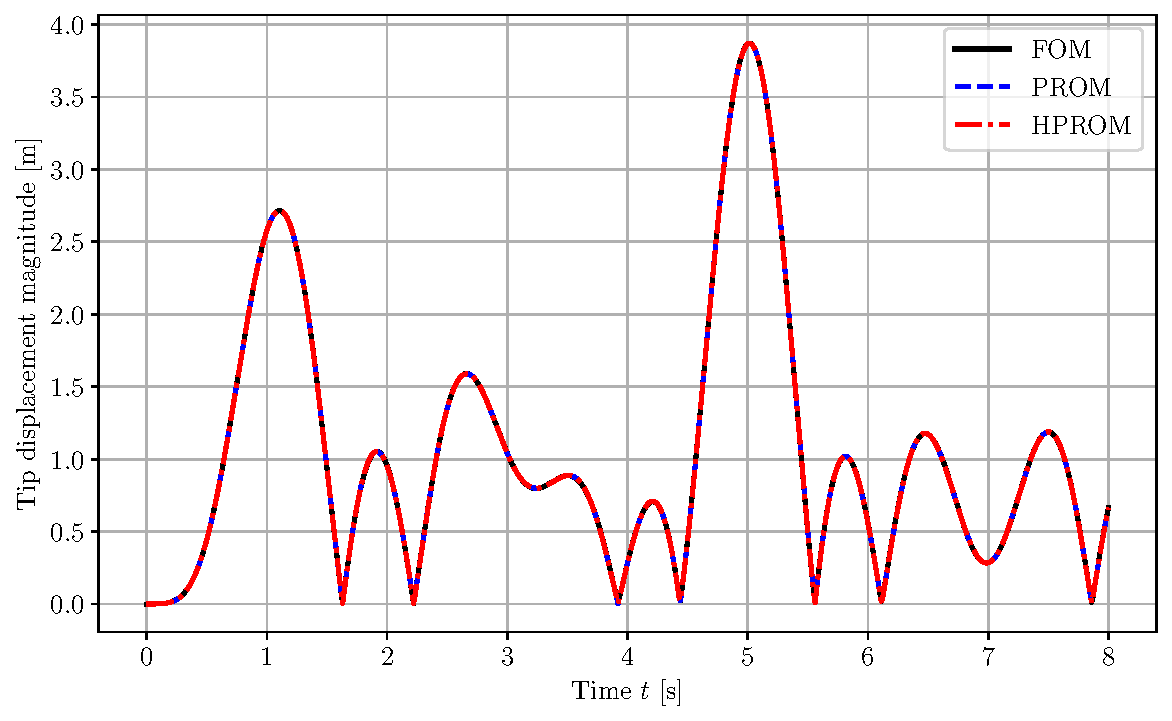
\includegraphics[width=0.75\textwidth]{Figures/tip_displacement_comparison.pdf}
    \caption{
    Time evolution of the wind turbine blade tip displacement under the test loading condition.
    }
    \label{fig:fom_vs_rom_tip}
\end{figure}

\begin{figure}[ht!]
    \centering

    % t = 1s
    \begin{subfigure}[b]{0.3\textwidth}
        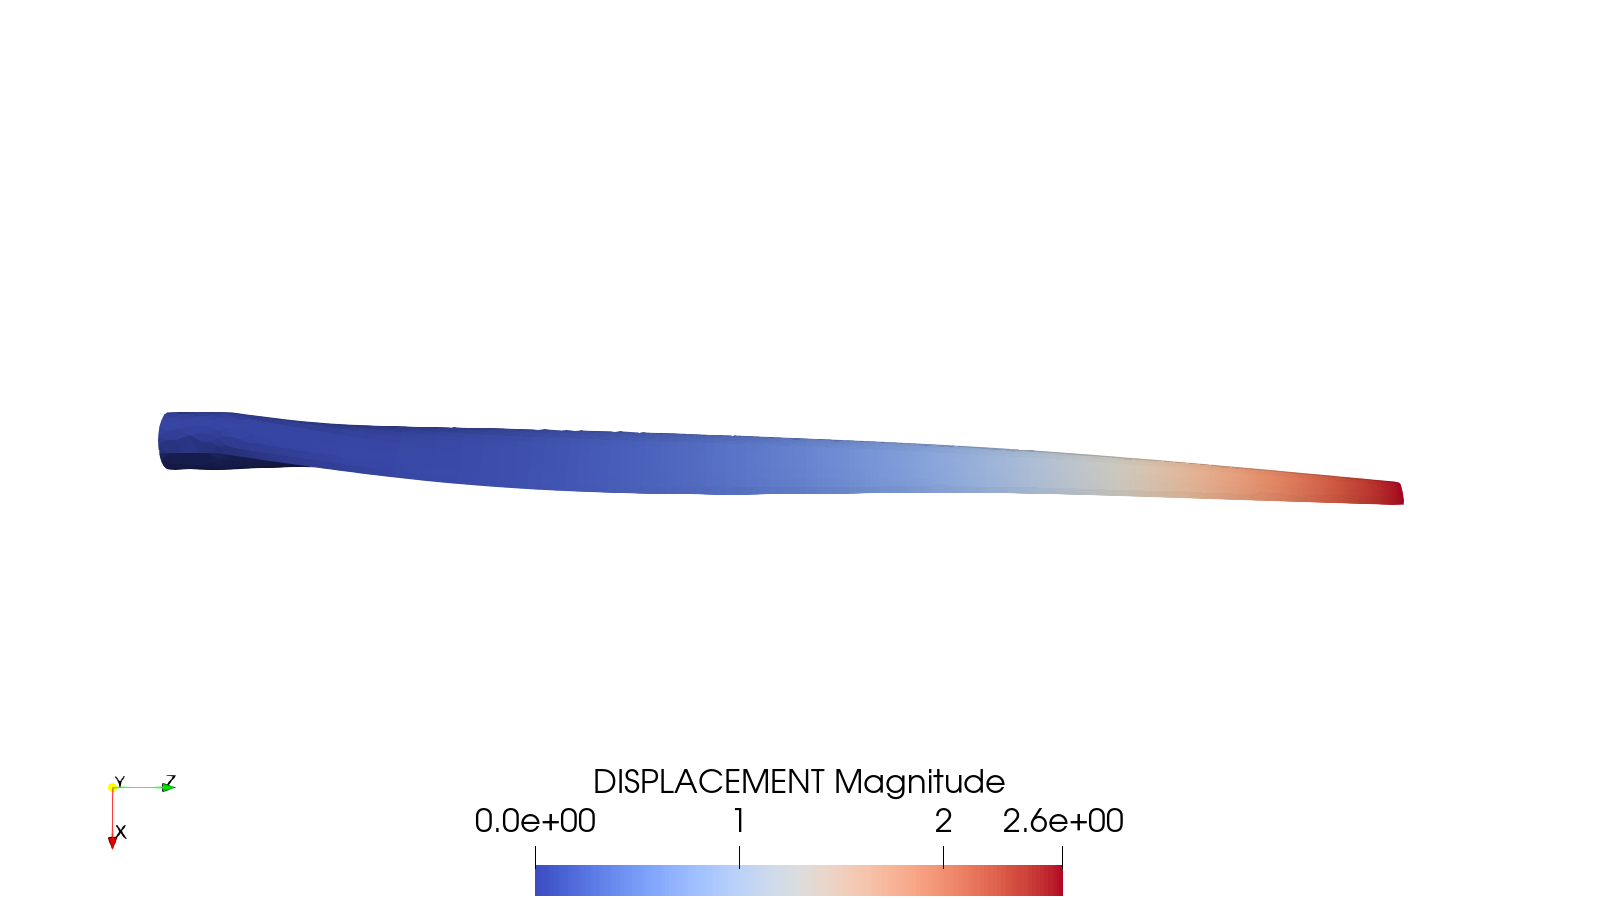
\includegraphics[width=\textwidth]{Figures/fom_t1.png}
        \caption{FOM at \(t = 1\,\text{s}\)}
    \end{subfigure}
    \hfill
    \begin{subfigure}[b]{0.3\textwidth}
        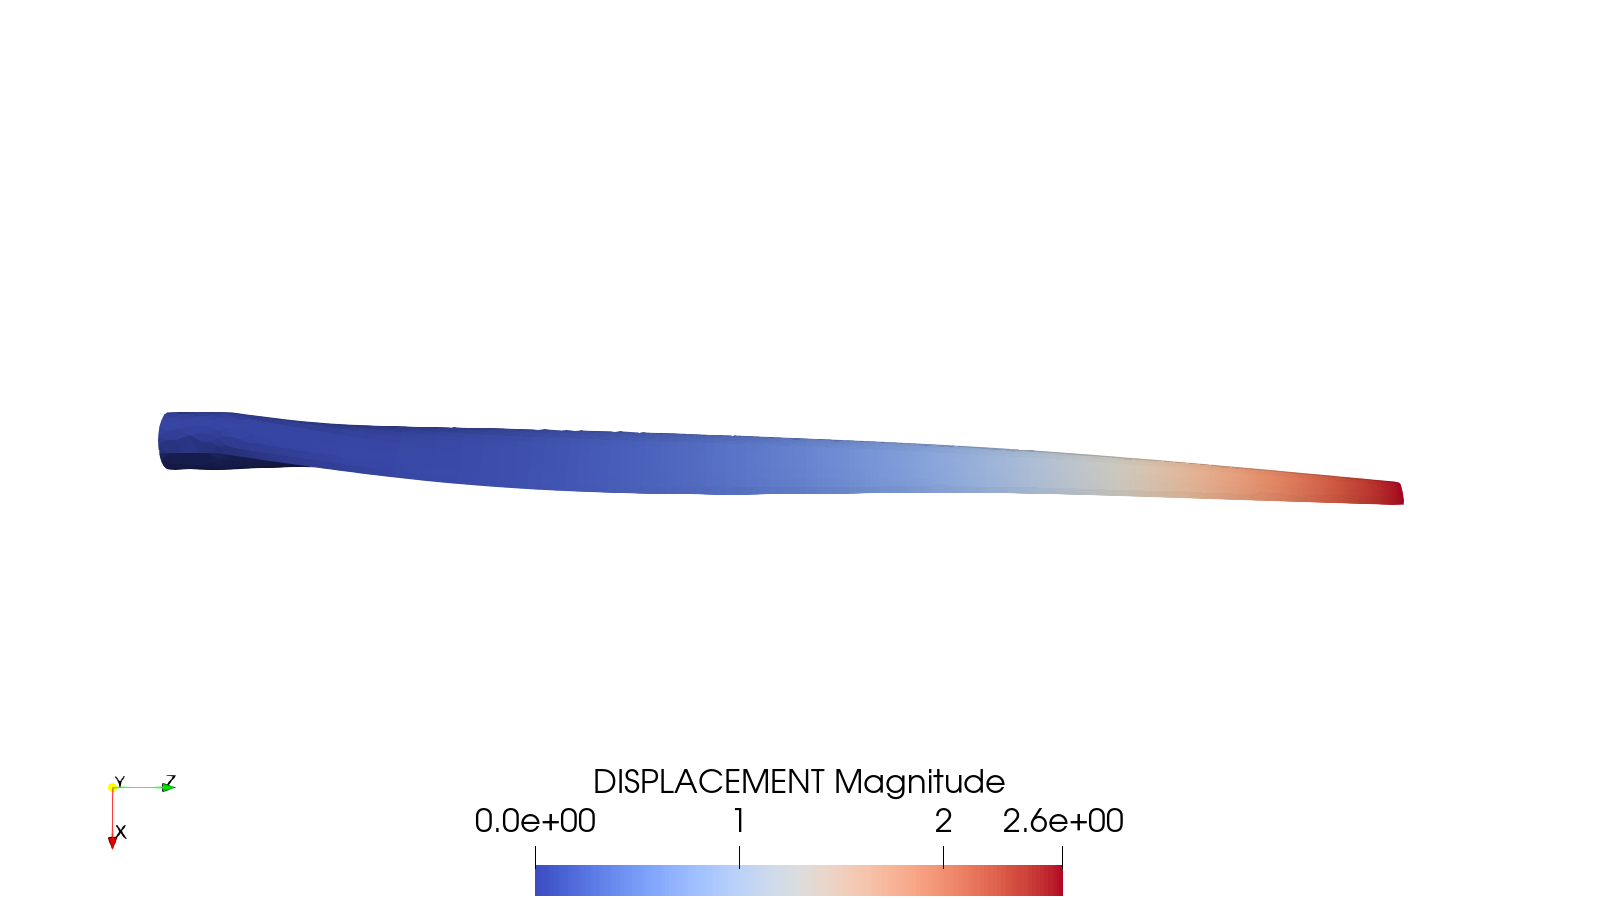
\includegraphics[width=\textwidth]{Figures/prom_t1.png}
        \caption{PROM at \(t = 1\,\text{s}\)}
    \end{subfigure}
    \hfill
    \begin{subfigure}[b]{0.3\textwidth}
        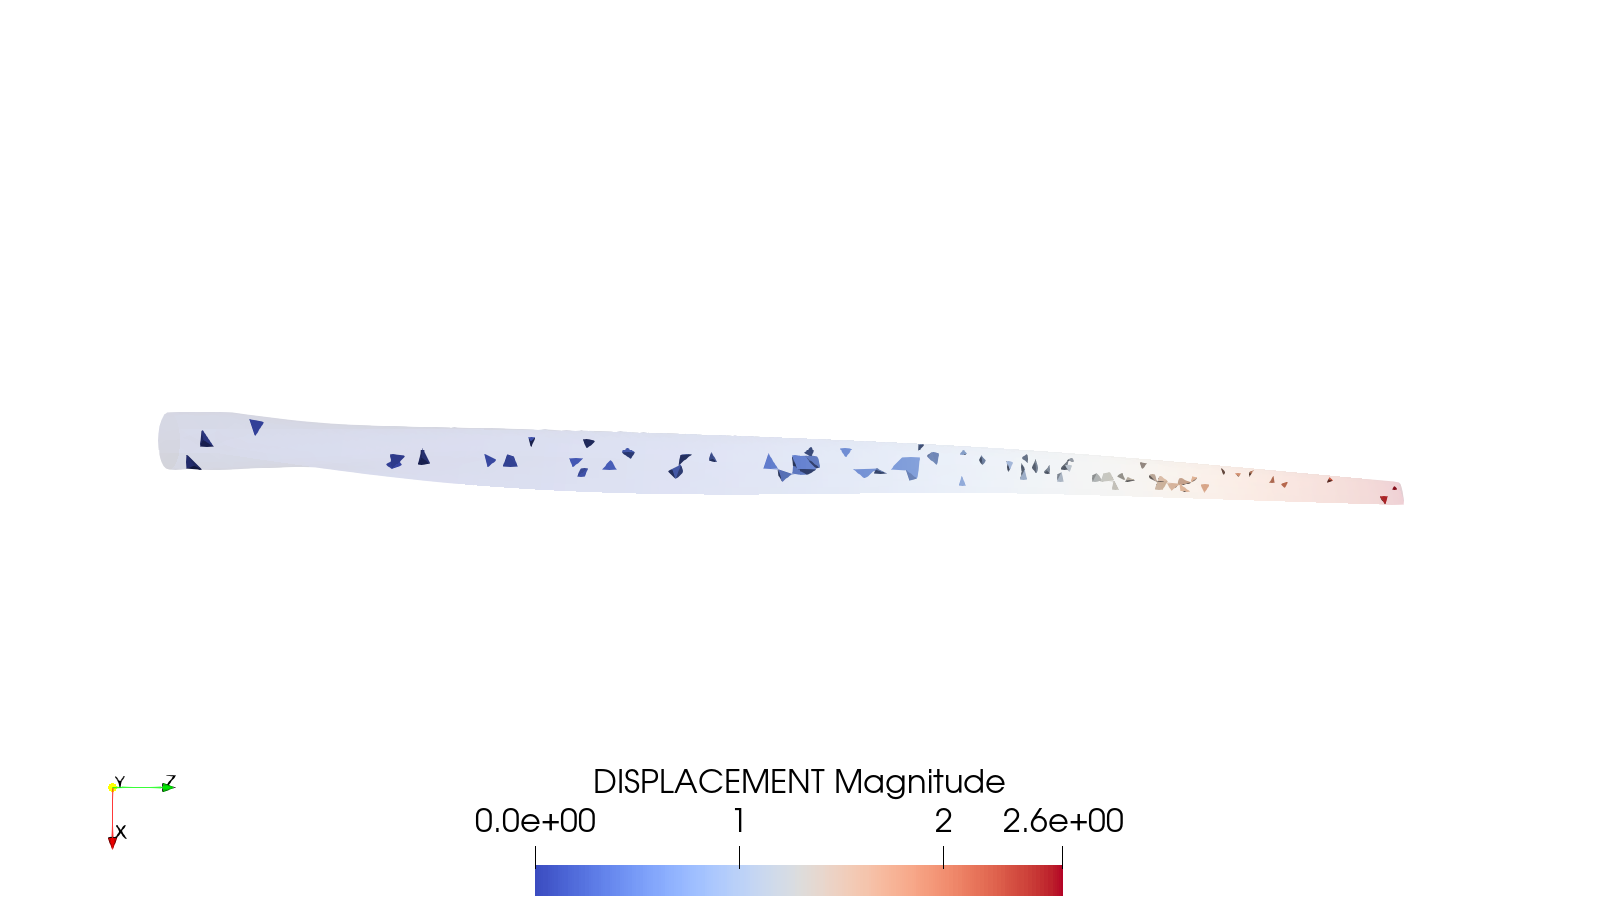
\includegraphics[width=\textwidth]{Figures/hprom_t1.png}
        \caption{HPROM at \(t = 1\,\text{s}\)}
    \end{subfigure}

    \vspace{1em}

    % t = 5s
    \begin{subfigure}[b]{0.3\textwidth}
        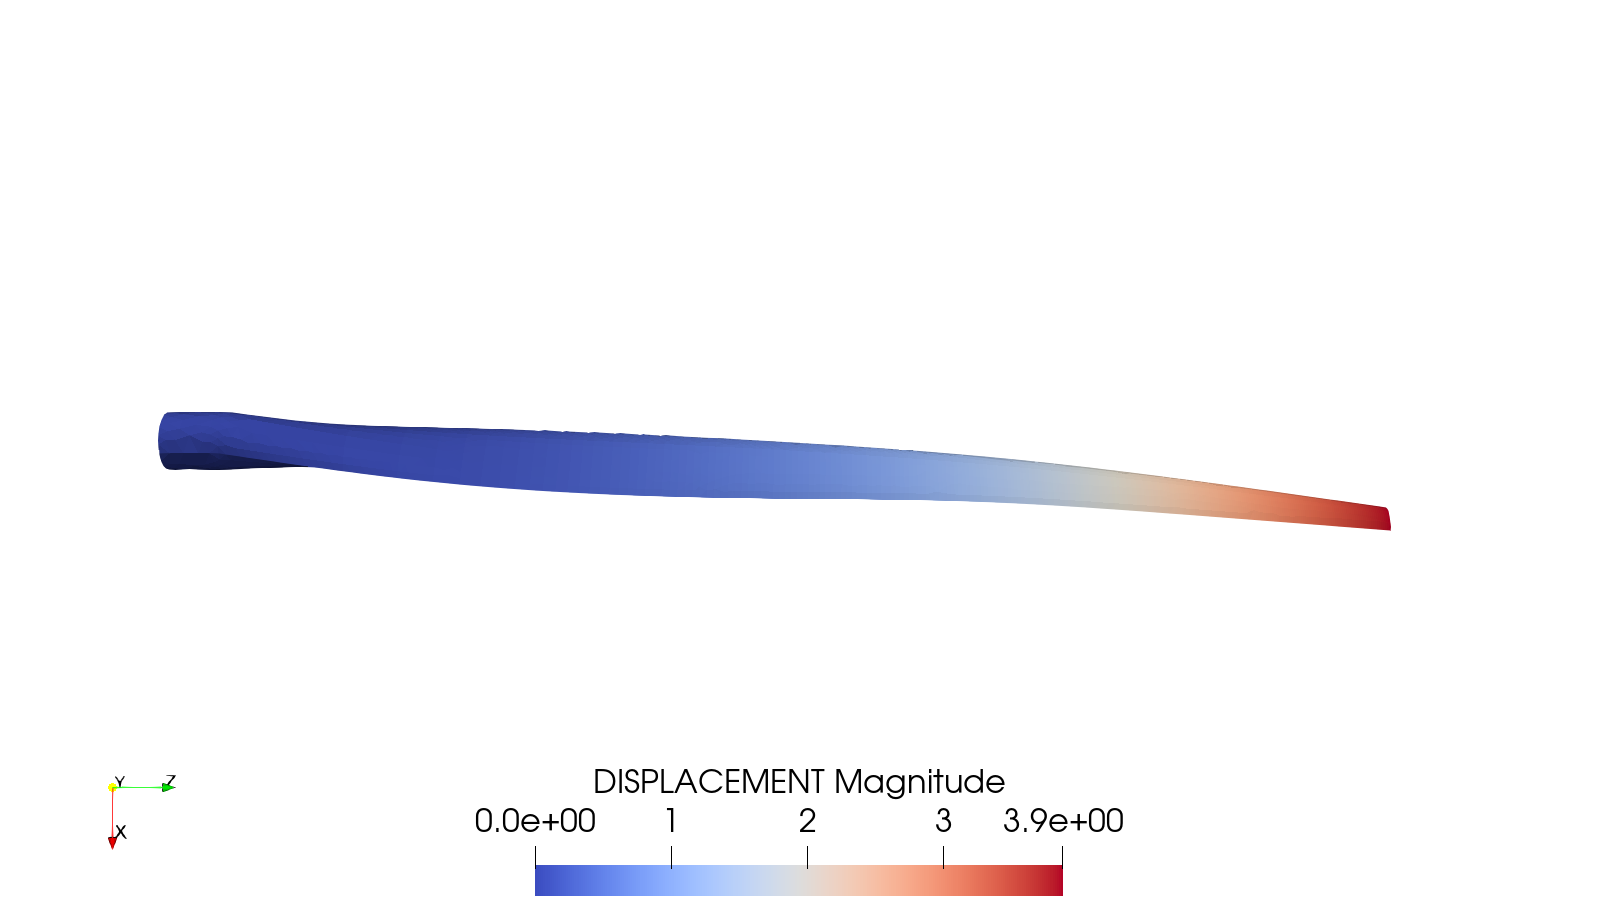
\includegraphics[width=\textwidth]{Figures/fom_t5.png}
        \caption{FOM at \(t = 5\,\text{s}\)}
    \end{subfigure}
    \hfill
    \begin{subfigure}[b]{0.3\textwidth}
        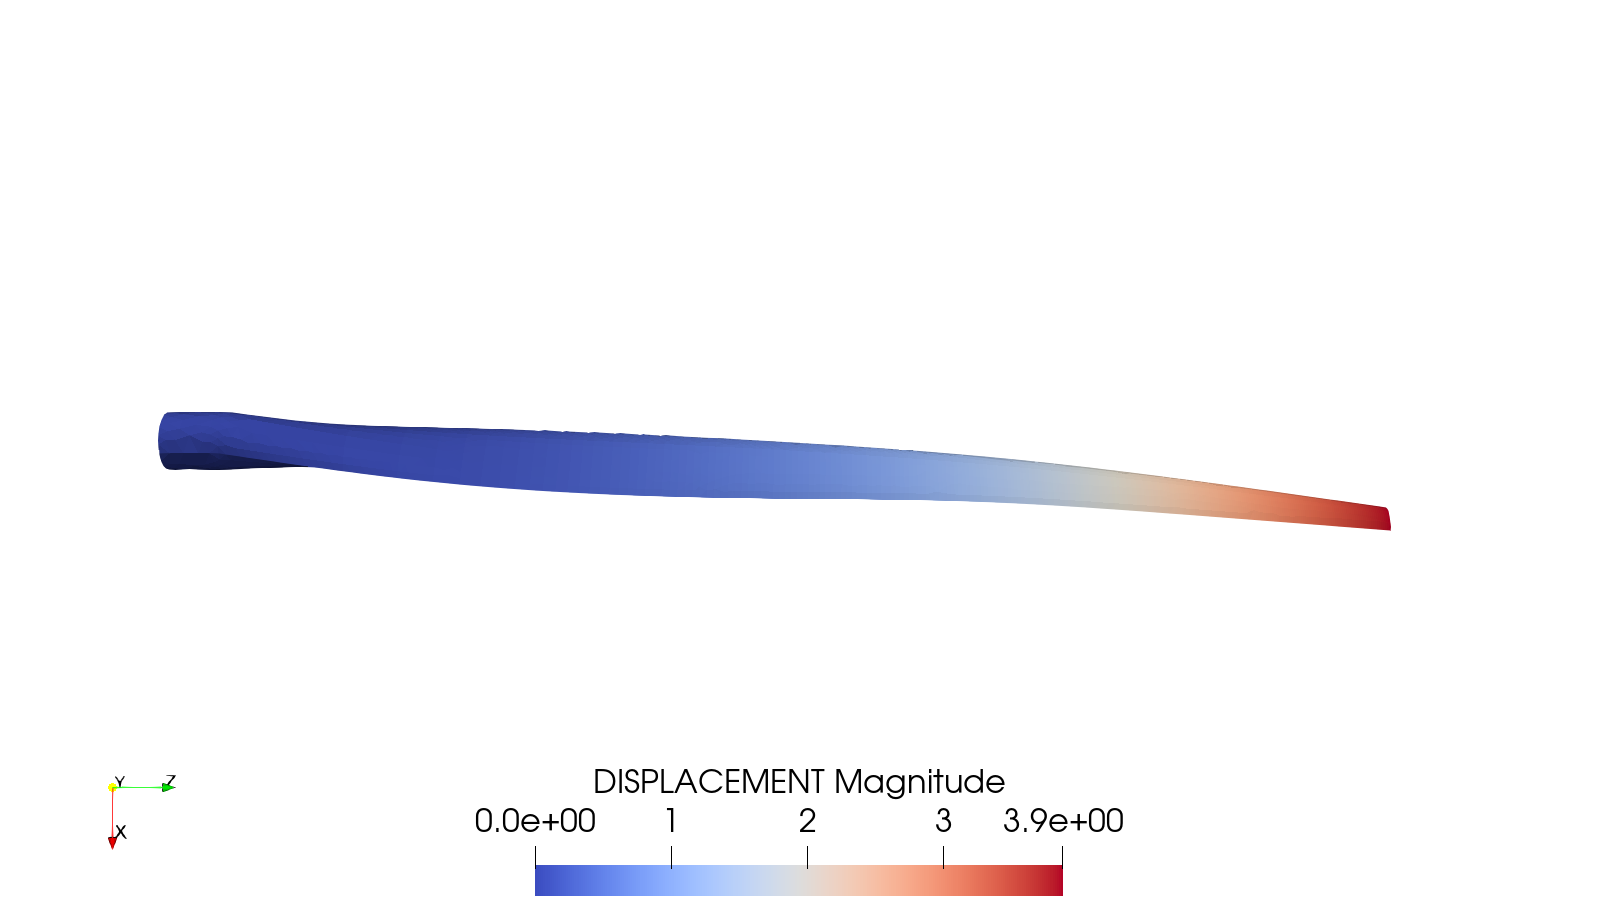
\includegraphics[width=\textwidth]{Figures/prom_t5.png}
        \caption{PROM at \(t = 5\,\text{s}\)}
    \end{subfigure}
    \hfill
    \begin{subfigure}[b]{0.3\textwidth}
        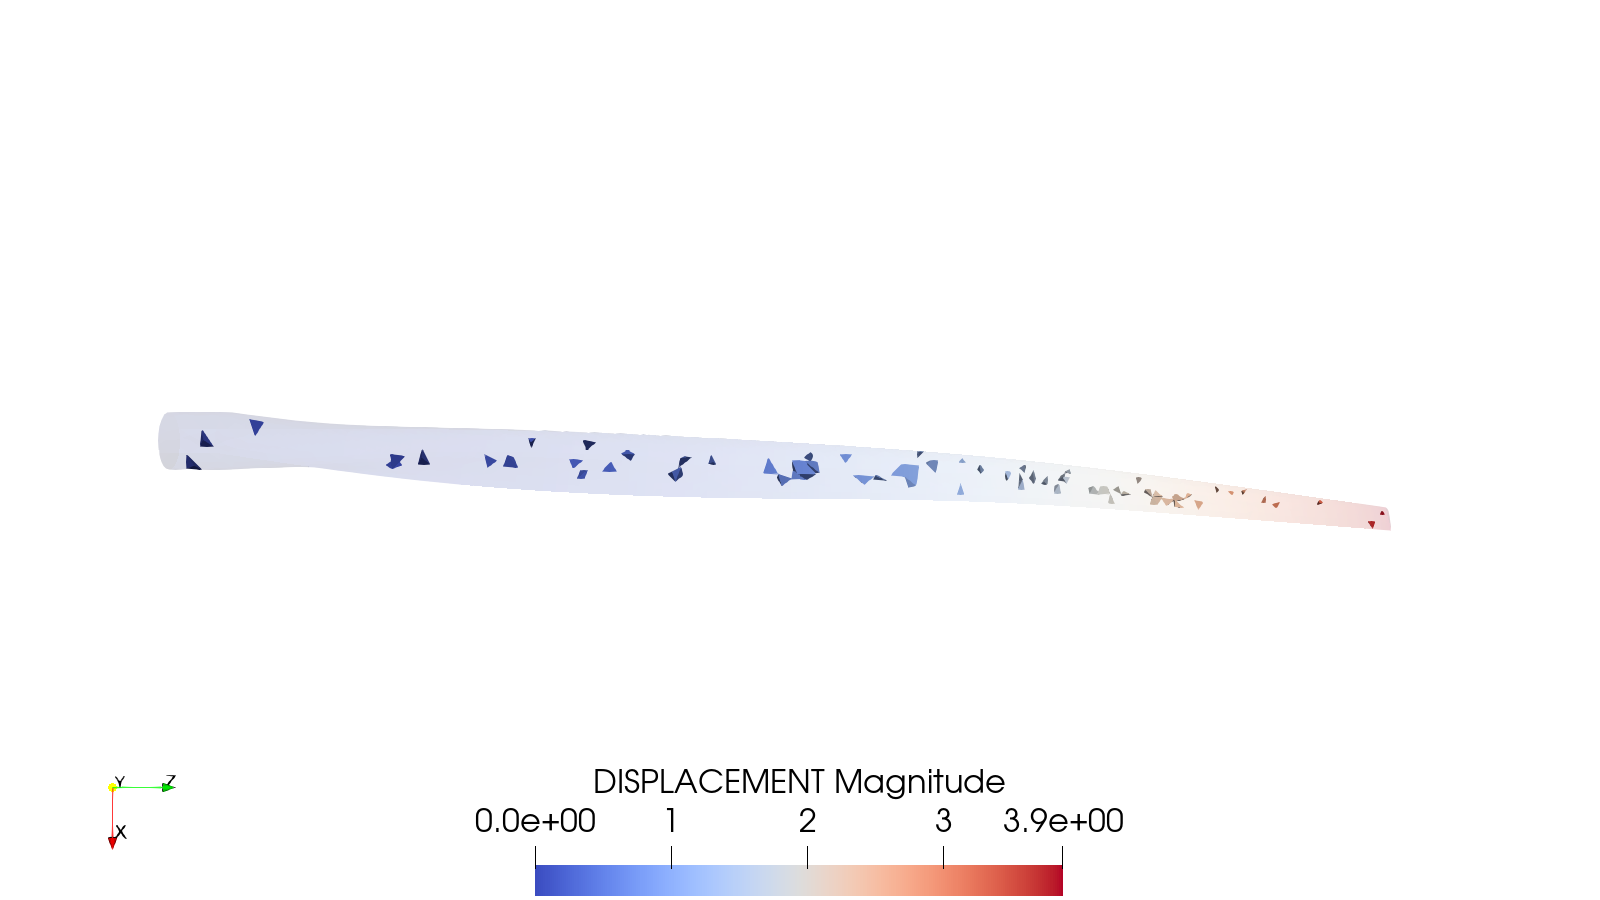
\includegraphics[width=\textwidth]{Figures/hprom_t5.png}
        \caption{HPROM at \(t = 5\,\text{s}\)}
    \end{subfigure}

    \caption{
    Spatial displacement fields of the wind turbine blade at two representative time instants during the test case simulation. Each row compares the FOM, PROM, and HPROM.
    }
    \label{fig:fom_rom_snapshots}
\end{figure}

\noindent
While the results confirm the effectiveness of POD-Galerkin for symmetric positive-definite problems, the next section shows that convection-dominated systems require a more robust projection, motivating the shift toward the LSPG framework.

\paragraph{Remark on industrial scalability.}
While the wind turbine blade example is solved efficiently using projection-based model reduction and hyper-reduction, it remains a relatively modest case in terms of size and parametric complexity. Nevertheless, it is derived from an actual industrial geometry and loading profile, and thus serves as a meaningful benchmark. In realistic engineering scenarios, featuring finer meshes, longer simulation horizons, richer material models, and high-dimensional parameter spaces, the offline construction of reduced-order models (e.g., snapshot generation, POD, and hyper-reduction via ECM) becomes a significant computational burden. These considerations motivate the need for parallel, HPC-enabled workflows to support scalable PROM construction for real-time digital twin applications. This broader perspective is discussed and addressed in the paper presented in Chapter~\ref{chap:article2}.

\section{Linear POD PROM for the model problem}
\label{sec:pod_prom_burgers}

\subsection{Parametric model problem and PROM setup}
\label{subsec:burgers_parametric_setup}

To evaluate the performance of linear subspace PROMs in convection-dominated regimes, the inviscid one-dimensional Burgers’ equation with a parametric source term is employed. This hyperbolic model problem, introduced in Chapter~\ref{sec:model_problem}, exhibits nonlinear wave propagation, shock formation, and non-symmetric residual operators, hallmarks of first-order hyperbolic PDEs that challenge standard projection methods due to their sharp gradients, low regularity, and parameter sensitivity.

For clarity of exposition, the governing equation is reprinted below in its parametric form:
\begin{equation}
\frac{\partial u}{\partial t} + u \frac{\partial u}{\partial x} = f(x; \mu_2),
\qquad
u(0, t) = \mu_1,
\label{eq:burgers_parametric}
\end{equation}
where \( \mu_1 \) denotes the left Dirichlet boundary condition, and \( \mu_2 \) modulates the spatial amplitude of the source term \( f(x; \mu_2) \). The full derivation of this model, including the weak form, finite element discretization with SUPG stabilization, time integration, and residual formulation, is presented in Section~\ref{sec:fem_discretization}.

The spatial domain \([0, 100]\) is discretized using 511 linear finite elements, yielding 512 nodes and therefore \( N = 512 \) spatial degrees of freedom. This discretization matches the setup introduced in Chapter~\ref{sec:model_problem} and is retained consistently throughout the PROM development.

The parametric domain is defined as
\[
\mathcal{D} = [4.25, 5.50] \times [0.015, 0.030],
\]
and is discretized using a uniform \( 3 \times 3 \) Cartesian grid (see Figure~\ref{fig:burgers_param_grid}), resulting in nine parameter configurations. For each \(\boldsymbol{\mu} \in \mathcal{D}\), a high-fidelity simulation is performed using backward Euler time integration and Newton–Raphson solvers, as described in Section~\ref{sec:fem_discretization}. Each trajectory consists of 500 time steps plus the initial condition, yielding 501 snapshots per parameter combination and resulting in the snapshot matrix \( \mathbf{S} \in \mathbb{R}^{N \times 4509} \).

\begin{figure}[ht!]
    \centering
    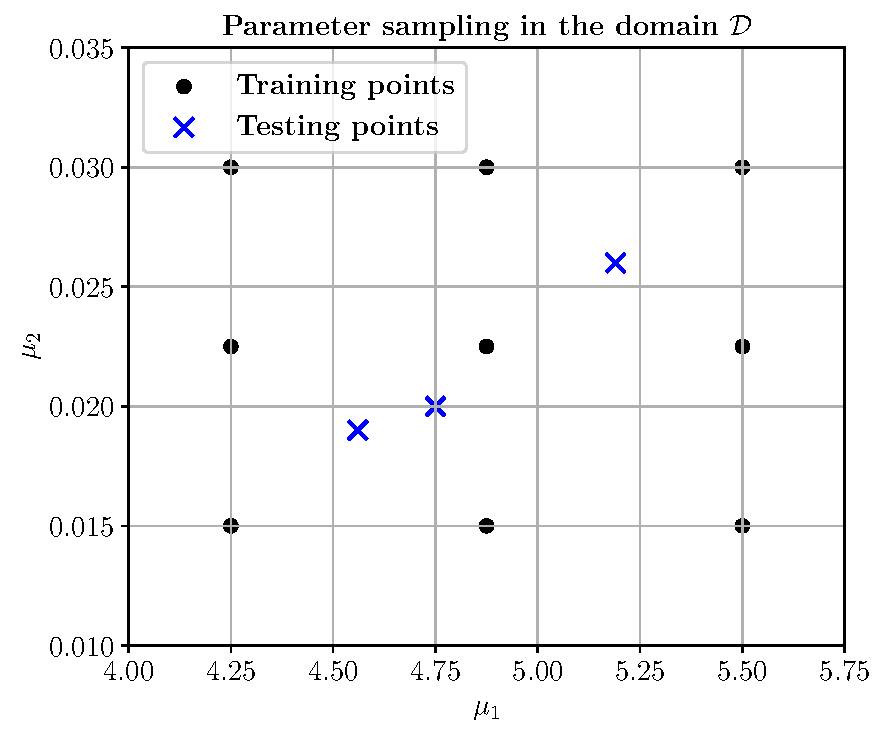
\includegraphics[width=0.65\textwidth]{Figures/parametric_domain.pdf}
    \caption{
        Training parameter combinations (black dots) and test configurations (blue crosses) in the parametric domain \( \mathcal{D} \subset \mathbb{R}^2 \).
    }
    \label{fig:burgers_param_grid}
\end{figure}

The nine training points \( \{\boldsymbol{\mu}^{(i)}_{\text{train}}\}_{i=1}^{9} \) form the basis of the offline stage for projection-based model reduction. In addition, three out-of-sample test configurations are selected within the domain to assess the generalization performance of the resulting PROM.

\subsection{Spectral decay and POD basis structure}
\label{subsec:pod_basis_structure}

The snapshot matrix \( \mathbf{S} \in \mathbb{R}^{N \times 4509} \), constructed from nine high-fidelity simulations across the parametric domain, is decomposed via SVD. The resulting singular values \( \{ \sigma_i \} \) quantify the projection error associated with truncating the left singular vectors, which define the reduced basis.

Figure~\ref{fig:singular_value_decay} presents the cumulative relative loss in linear energy as a function of the retained singular value index. The decay is notably slow, confirming that a high number of modes is required to achieve low approximation errors. This flat spectrum is a consequence of nonlinear transport phenomena, sharp wavefronts, and parametric variability, which reduce the compressibility of the solution manifold. This behavior is consistent with a system characterized by a high \emph{Kolmogorov \( n \)-width}~\cite{pinkus2012n}.

The vertical lines in Figure~\ref{fig:singular_value_decay} indicate the number of modes \( n \) needed to achieve different tolerance thresholds. Table~\ref{tab:mode_counts} summarizes the exact mode counts for the tolerances 
\[ \epsilon^2 = \{10^{-2}, 10^{-3}, 10^{-4}, 10^{-5}, 10^{-6}\}. \]

\begin{figure}[htbp]
    \centering
    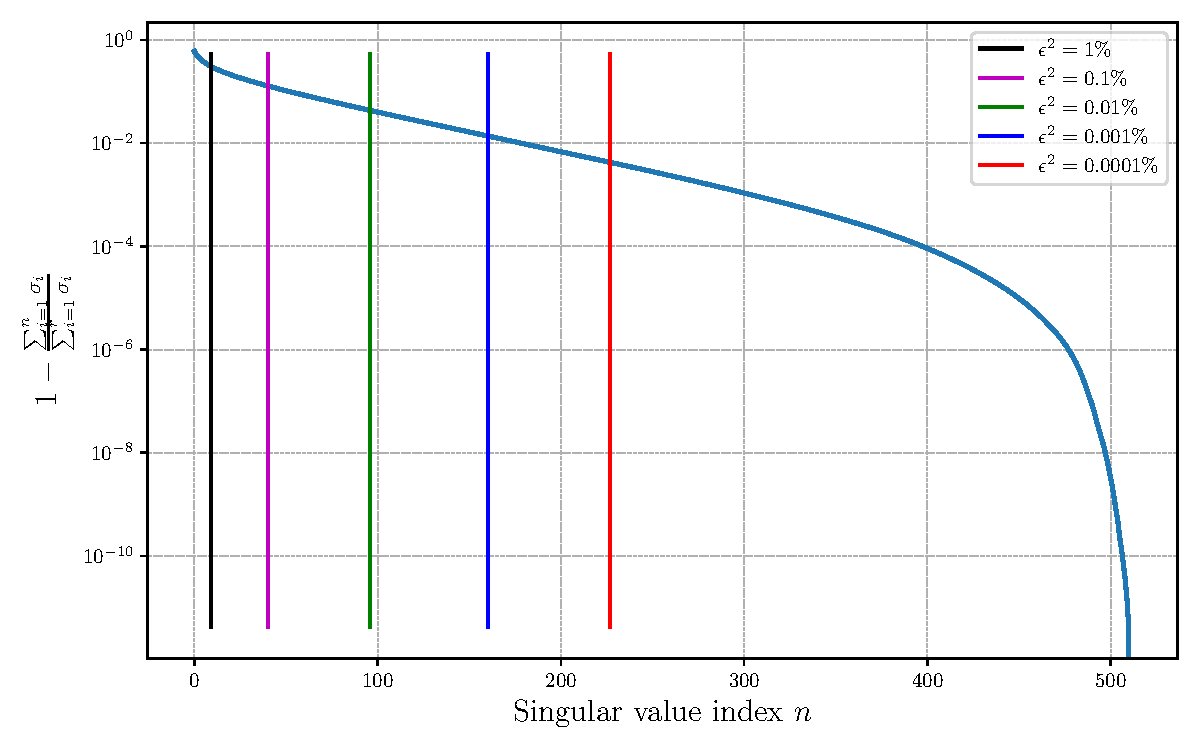
\includegraphics[width=0.7\textwidth]{Figures/singular_value_decay_linear_loss.pdf}
    \caption{Cumulative relative energy loss \( 1 - \sum_{i=1}^n \sigma_i / \sum_{i=1}^r \sigma_i \) for increasing number of retained singular values \( n \). Threshold lines show mode counts for selected tolerances \( \epsilon^2 \).}
    \label{fig:singular_value_decay}
\end{figure}

\begin{table}[!htbp]
    \centering
    \begin{tabular}{c|ccccc}
        \toprule
        \( \epsilon^2 \) & \( 10^{-2} \) & \( 10^{-3} \) & \( 10^{-4} \) & \( 10^{-5} \) & \( 10^{-6} \) \\
        \midrule
        \( n \) & 9 & 40 & 96 & 160 & 227 \\
        \bottomrule
    \end{tabular}
    \caption{Number of retained modes \( n \) for different squared tolerance thresholds \( \epsilon^2 \).}
    \label{tab:mode_counts}
\end{table}

Figure~\ref{fig:first6_pod_modes} displays the first six left singular vectors (POD modes). The modes exhibit increasing spatial oscillations and steepening fronts, aligned with the structure of propagating nonlinear waves.

\begin{figure}[!htbp]
    \centering
    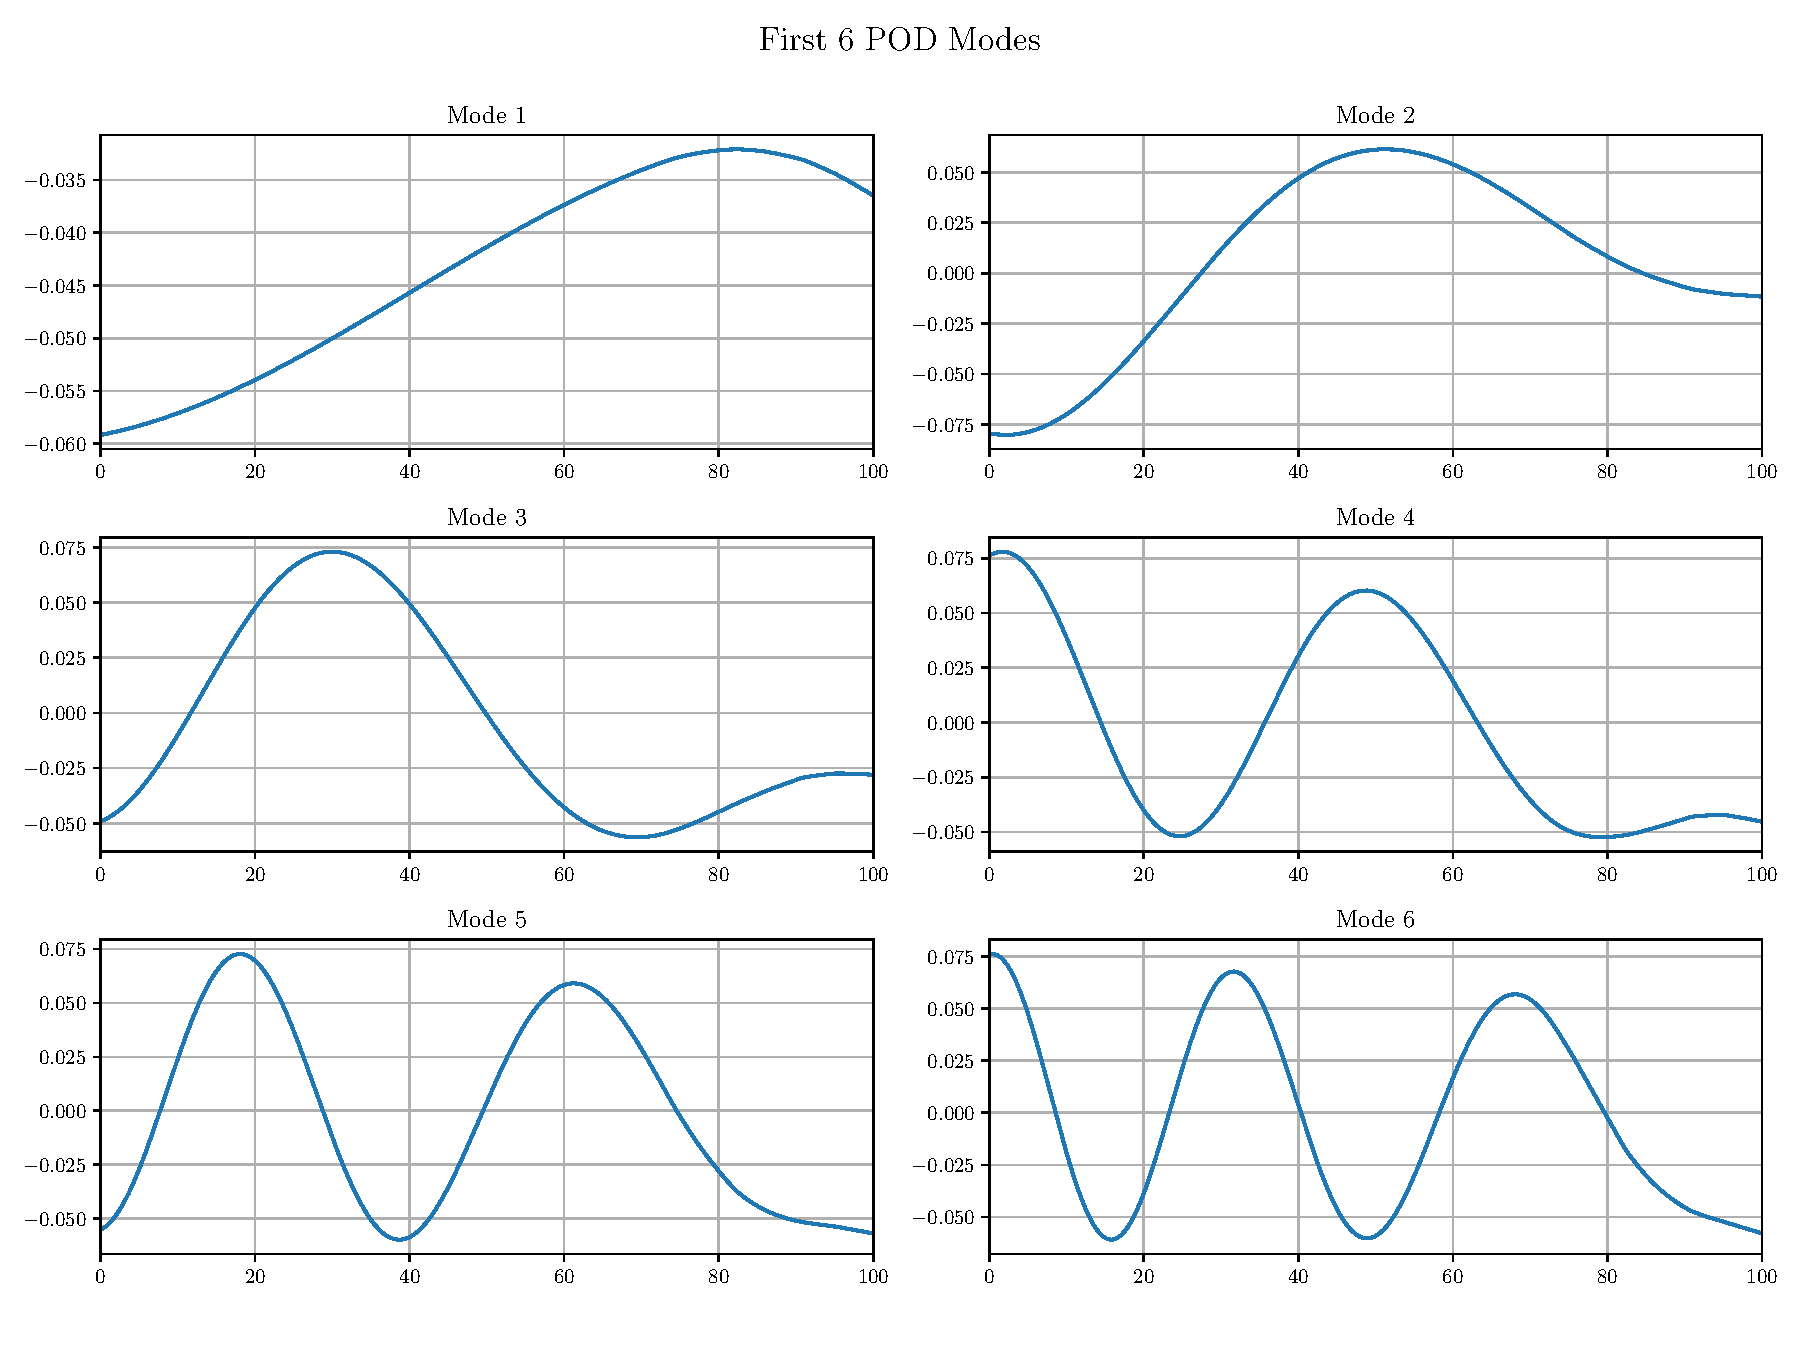
\includegraphics[width=0.75\textwidth]{Figures/first_6_modes.pdf}
    \caption{First six POD modes extracted from the SVD of the snapshot matrix. Each mode is defined over the domain \( x \in [0,100] \) with \( N = 512 \) spatial degrees of freedom.}
    \label{fig:first6_pod_modes}
\end{figure}

\subsection{Galerkin vs. LSPG projection for PROMs and the limitations of linear subspaces}
\label{subsec:galerkin_lspg_comparison}

Although the Galerkin projection offers optimality guarantees for symmetric positive-definite (SPD) operators, in convection-dominated flows, such as the one-dimensional inviscid Burgers equation considered here, the system operators are non-symmetric and dominated by transport terms, leading to suboptimal performance and potential instabilities with the Galerkin projection~\cite{carlberg2011efficient, carlberg2017galerkin}.

To address these limitations, the LSPG formulation replaces the orthogonality condition with a residual minimization principle, solving at each time step and parameter instance the nonlinear least-squares problem:
\begin{equation}
\min_{\mathbf{q}(t,\boldsymbol{\mu})} \; 
\tfrac{1}{2} \left\| 
\mathbf{R}\bigl(\boldsymbol{\Phi}\,\mathbf{q}(t,\boldsymbol{\mu});\,t,\boldsymbol{\mu}\bigr) 
\right\|_2^2.
\end{equation}
This optimization yields the first-order optimality condition
\begin{equation}\label{eq:lspg_residual}
\boldsymbol{\Phi}^{\!T}\,
\mathbf{J}^{\!T}\bigl(\boldsymbol{\Phi}\,\mathbf{q}(t,\boldsymbol{\mu});\,t,\boldsymbol{\mu}\bigr)\,
\mathbf{R}\bigl(\boldsymbol{\Phi}\,\mathbf{q}(t,\boldsymbol{\mu});\,t,\boldsymbol{\mu}\bigr)
= \mathbf{0},
\end{equation}
defining the LSPG reduced residual system
\begin{equation}
\mathbf{R}_{r}^{\text{LSPG}}\bigl(\mathbf{q}(t,\boldsymbol{\mu});\,t,\boldsymbol{\mu}\bigr) 
:= \boldsymbol{\Phi}^{\!T}\,
\mathbf{J}^{\!T}\bigl(\boldsymbol{\Phi}\,\mathbf{q}(t,\boldsymbol{\mu});\,t,\boldsymbol{\mu}\bigr)\,
\mathbf{R}\bigl(\boldsymbol{\Phi}\,\mathbf{q}(t,\boldsymbol{\mu});\,t,\boldsymbol{\mu}\bigr)
\;\in\; \mathbb{R}^n.
\end{equation}

This nonlinear reduced system is typically solved with Newton iterations, requiring the reduced LSPG Jacobian
\begin{equation}\label{eq:lspg_reduced_jacobian}
\mathbf{J}_{r}^{\text{LSPG}}\bigl(\mathbf{q}(t,\boldsymbol{\mu});\,t,\boldsymbol{\mu}\bigr) 
= \boldsymbol{\Phi}^{\!T}\,
\mathbf{J}^{\!T}\bigl(\boldsymbol{\Phi}\,\mathbf{q}(t,\boldsymbol{\mu});\,t,\boldsymbol{\mu}\bigr)\,
\mathbf{J}\bigl(\boldsymbol{\Phi}\,\mathbf{q}(t,\boldsymbol{\mu});\,t,\boldsymbol{\mu}\bigr)\,
\boldsymbol{\Phi}
\;\in\;\mathbb{R}^{n\times n}.
\end{equation}


The LSPG formulation enhances robustness for convection-dominated and non-SPD systems by relaxing the strict projection orthogonality and instead enforcing residual minimization in the full-order space (see Chapter~\ref{chap:article1} for a complete derivation).

To compare the performance of the Galerkin and LSPG projection methods, reduced-order solutions are evaluated for three test parameter configurations outside the training set: $\boldsymbol{\mu}_1 = [4.75,\, 0.0200]$, $\boldsymbol{\mu}_2 = [4.56,\, 0.0190]$, and $\boldsymbol{\mu}_3 = [5.19,\, 0.0260]$. Each model is tested across multiple truncation tolerances, and predictive accuracy is assessed through quantitative and qualitative comparisons with the corresponding FOM solutions.

\textbf{Quantitative assessment.}
To evaluate the predictive accuracy of the Galerkin and LSPG reduced-order models, the following relative error metric is adopted:
\begin{equation}
	\label{eq:error-metric}
	\mathbb{RE}_{2, \text{QoI}}(\boldsymbol{\mu}^\star) = 100\times \frac{\sqrt{\displaystyle \sum_{m=0}^{N_t} \left\|\,\text{QoI}_m(\boldsymbol{\mu^\star}) - \widetilde{\text{QoI}}_m (\boldsymbol{\mu^\star})\, \right \|_2^2}} {\sqrt{\sum\limits_{m=0}^{N_t} \left \|\,\text{QoI}_m (\boldsymbol{\mu^\star})\,\right\|_2^2}},
\end{equation}
where the quantity of interest (QoI) is the full solution vector $\mathbf{u}_m$, and the error is accumulated over the complete time horizon $[0, 25\,\text{s}]$.

Figure~\ref{fig:prom_multitols_finaltime} compares Galerkin and LSPG predictions against the FOM solution at final time $t = 25\,\text{s}$ for the test case $\boldsymbol{\mu}_2 = [4.56,\, 0.0190]$, across four different tolerances ($10^{-2}$ to $10^{-5}$). Both PROMs benefit from increasing basis resolution; however, LSPG consistently offers better agreement with the FOM for tolerances $\epsilon^2 \leq 10^{-3}$, while Galerkin suffers from visible post-shock oscillations.

\begin{figure}[htbp]
    \centering
    \begin{subfigure}{0.48\textwidth}
        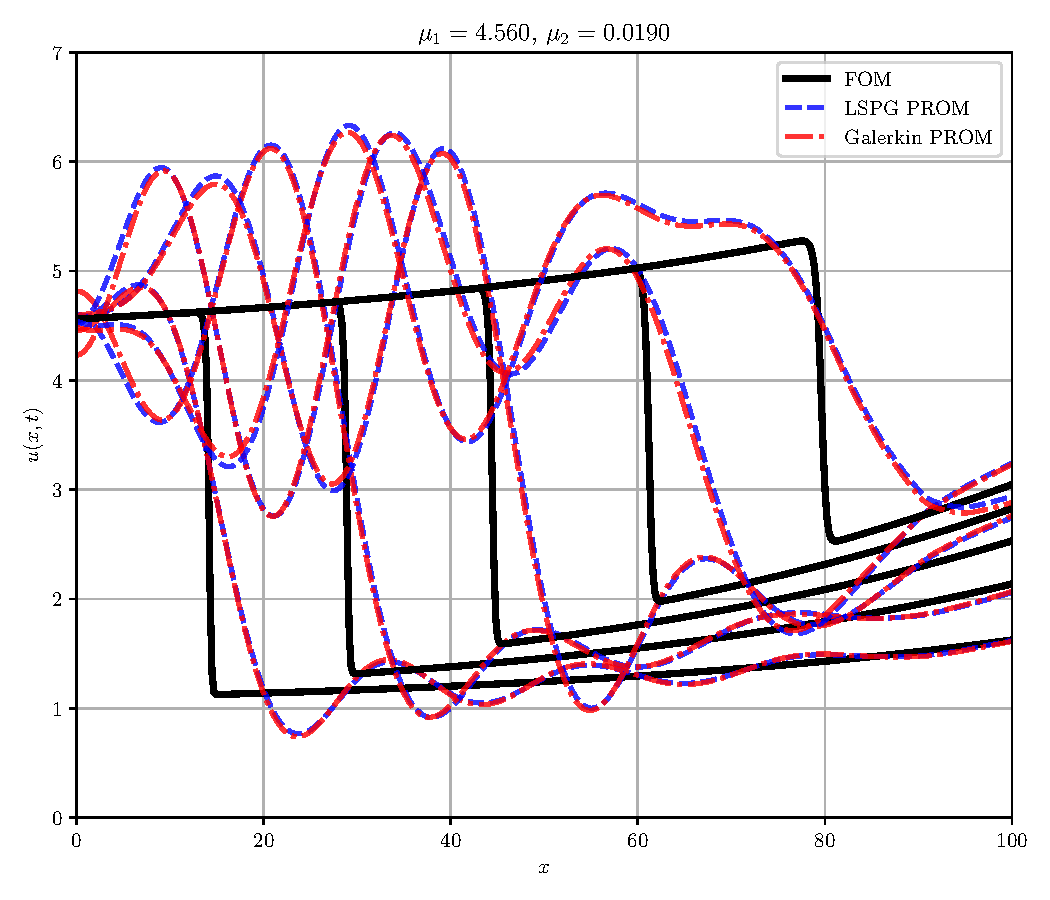
\includegraphics[width=\textwidth]{Figures/fom_pod_mu1_4.560_mu2_0.0190_tol_1e-02_modes_9.pdf}
        \caption{$\epsilon^2 = 10^{-2}$ ($n = 9$)}
    \end{subfigure}
    \hfill
    \begin{subfigure}{0.48\textwidth}
        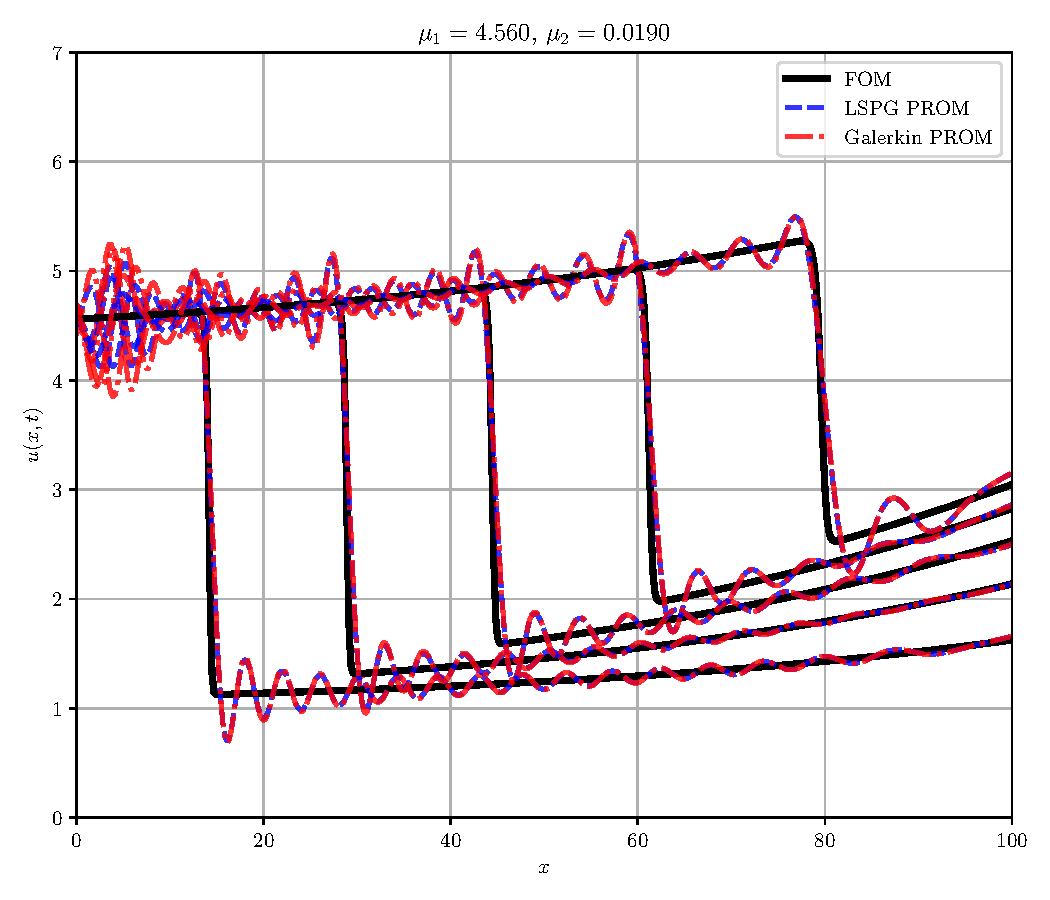
\includegraphics[width=\textwidth]{Figures/fom_pod_mu1_4.560_mu2_0.0190_tol_1e-03_modes_40.pdf}
        \caption{$\epsilon^2 = 10^{-3}$ ($n = 40$)}
    \end{subfigure}

    \vspace{0.5em}

    \begin{subfigure}{0.48\textwidth}
        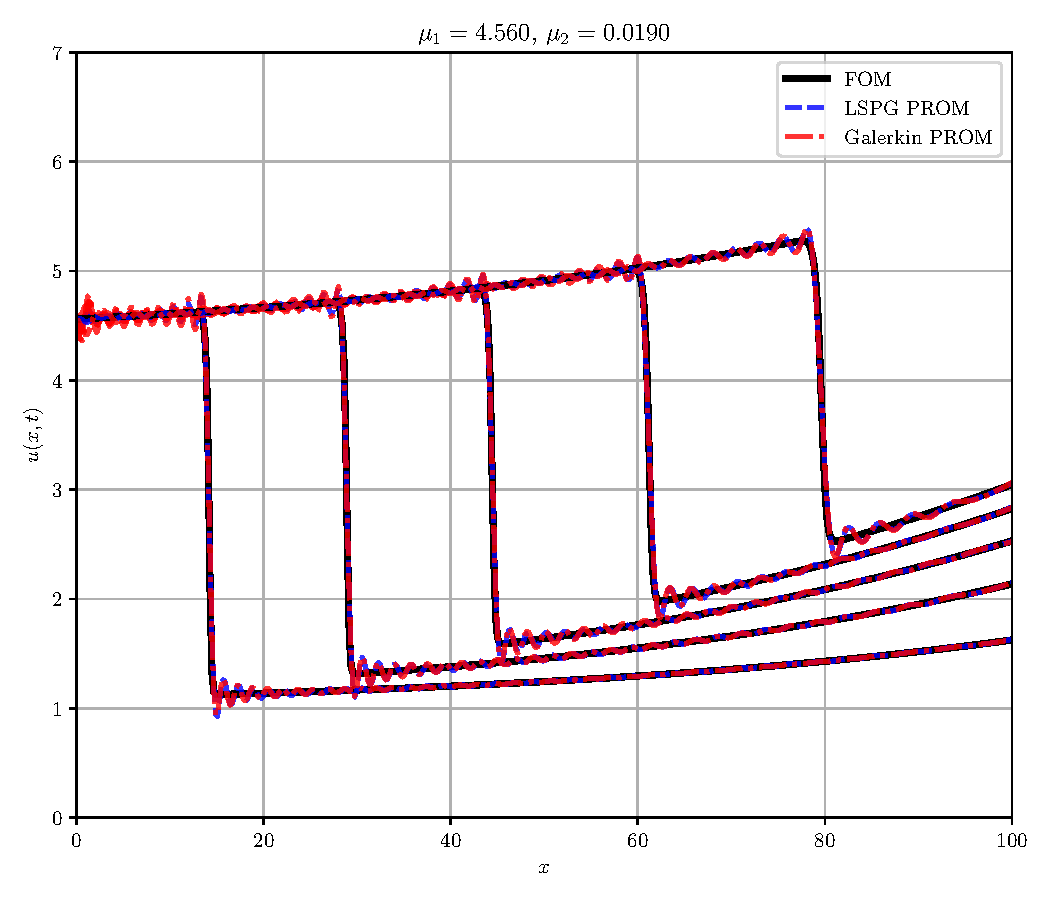
\includegraphics[width=\textwidth]{Figures/fom_pod_mu1_4.560_mu2_0.0190_tol_1e-04_modes_96.pdf}
        \caption{$\epsilon^2 = 10^{-4}$ ($n = 96$)}
    \end{subfigure}
    \hfill
    \begin{subfigure}{0.48\textwidth}
        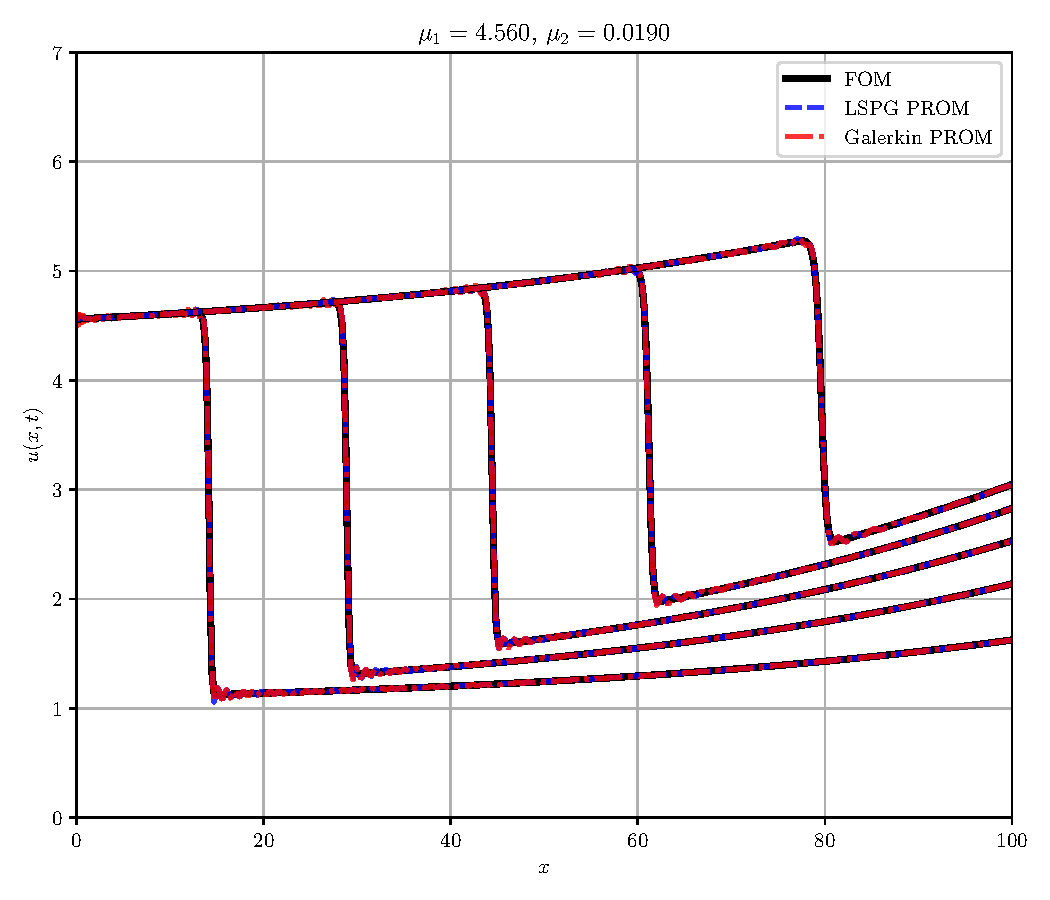
\includegraphics[width=\textwidth]{Figures/fom_pod_mu1_4.560_mu2_0.0190_tol_1e-05_modes_160.pdf}
        \caption{$\epsilon^2 = 10^{-5}$ ($n = 160$)}
    \end{subfigure}
    \caption{
        Galerkin and LSPG PROM predictions at $t = 25\,\text{s}$ for $\boldsymbol{\mu}^\star = [4.56,\, 0.0190]$ using different truncation tolerances. FOM reference is in black.
    }
    \label{fig:prom_multitols_finaltime}
\end{figure}

To summarize performance over all test cases, the maximum relative error is defined as:
\begin{equation*} 
	\mathbb{RE}_{2, \text{QoI}}^{\max} = \max_{\boldsymbol{\mu}_1, \boldsymbol{\mu}_2, \boldsymbol{\mu}_3} 
	\mathbb{RE}_{2, \text{QoI}} (\boldsymbol{\mu}),
\end{equation*}
and report it for each projection method and tolerance in Table~\ref{tab:prom_errors_summary}. The LSPG method outperforms Galerkin in all but the most severe truncation ($\epsilon^2 = 10^{-2}$), where the PROM dimension is insufficient to capture key features of the dynamics. Across all other settings, LSPG consistently yields lower maximum errors.

\begin{table}[!htbp]
    \centering
    \begin{tabular}{c c c c}
        \toprule
        \begin{tabular}[c]{@{}c@{}}Tolerance\\ $\epsilon^2$\end{tabular} & 
        \begin{tabular}[c]{@{}c@{}}Modes\\ $n$\end{tabular} & 
        \begin{tabular}[c]{@{}c@{}}Galerkin\\ $\mathbb{RE}_{2, \mathbf{u}}^{\max}$ (\%)\end{tabular} & 
        \begin{tabular}[c]{@{}c@{}}LSPG\\ $\mathbb{RE}_{2, \mathbf{u}}^{\max}$ (\%)\end{tabular} \\
        \midrule
        \( 10^{-2} \)  & 9    & 20.70 & 21.60 \\
        \( 10^{-3} \)  & 40   & 5.46  & 4.60  \\
        \( 10^{-4} \)  & 96   & 1.27  & 1.09  \\
        \( 10^{-5} \)  & 160  & 0.35  & 0.33  \\
        \( 10^{-6} \)  & 210  & 0.10  & 0.10  \\
        \bottomrule
    \end{tabular}
    \caption{Maximum relative error across three test configurations for Galerkin and LSPG PROMs at final time.}
    \label{tab:prom_errors_summary}
\end{table}

\textbf{Qualitative assessment.}
Figure~\ref{fig:prom_comparison_test1} shows the predicted solution at $t = 5\,\text{s}$ for the test configuration $\boldsymbol{\mu} = [4.75,\, 0.0200]$, using a reduced basis constructed with $\epsilon^2 = 10^{-4}$ (i.e., $n = 96$ modes). Both Galerkin and LSPG PROMs exhibit noticeable oscillations near the moving shock and in the post-shock region, reflecting the limitations of fixed linear subspaces in representing sharp, transport-dominated dynamics, an issue that arises independently of the projection method (i.e., standard POD reconstruction).
While neither approach yields highly accurate reconstructions, the LSPG projection consistently achieves slightly lower amplitude deviations compared to Galerkin.

These discrepancies are attributed to the residual-minimizing nature of LSPG, which improves robustness for hyperbolic, non-symmetric problems. Although the benefits of LSPG are moderate in this moderately reduced setting, the differences become more consequential in challenging configurations. In particular, while both PROMs remain stable in this benchmark case, the suboptimality of Galerkin can lead to unstable behavior or even numerical blow-up in more sensitive or industrial-scale applications, such as turbulent compressible flow simulations~\cite{carlberg2017galerkin}, underscoring the importance of careful projection design.

Altogether, these observations highlight the fundamental limitations imposed by the Kolmogorov $n$-width barrier when relying on linear trial subspaces. While increasing the number of modes can eventually improve accuracy (e.g., by reducing oscillations in the present case), overcoming the barrier often demands retaining an impractically large basis, which defeats the purpose of reduced-order modeling. \textbf{This motivates the transition to nonlinear manifold projection-based reduced-order models}, which relax the linear subspace constraint to better capture complex dynamics, a direction developed in detail in Chapter~\ref{chap:nonlinear_prom}. Furthermore, the improved performance of the LSPG projection reinforces its suitability for convection-dominated systems governed by non-symmetric operators (e.g., Navier--Stokes), where Galerkin projection may lead to unstable or inaccurate predictions.


\begin{figure}[ht!]
    \centering
    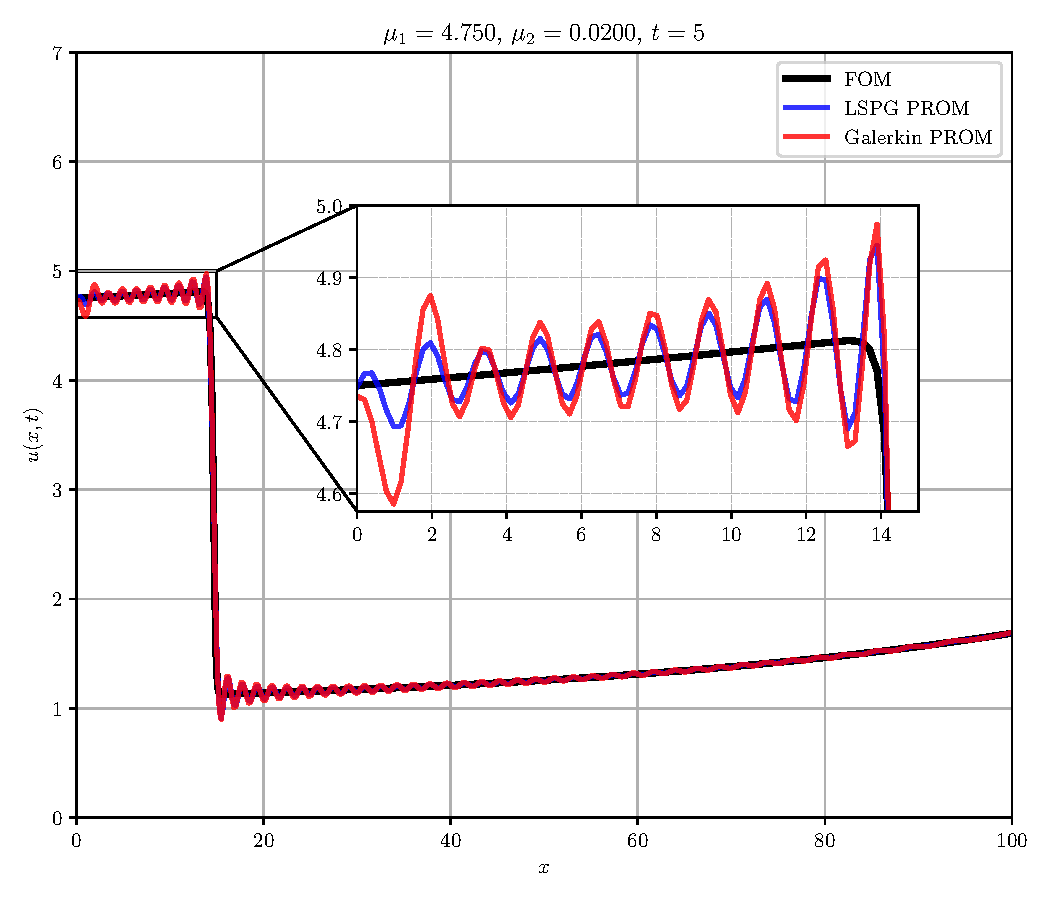
\includegraphics[width=0.7\textwidth]{Figures/fom_pod_comparison_tol_1e-04_mu1_4.750_mu2_0.0200_modes_96.pdf}
    \caption{Comparison of Galerkin and LSPG predictions at $t = 5\,\text{s}$ for $\boldsymbol{\mu} = [4.75,\, 0.0200]$, using a reduced basis with $n = 96$ modes ($\epsilon^2 = 10^{-4}$). LSPG exhibits slightly better agreement with the FOM, though both models show oscillations.}
    \label{fig:prom_comparison_test1}
\end{figure}

\section{Toward a Petrov--Galerkin framework and HPC-enabled training for industrial-scale applications}

The studies presented in this chapter underscore two complementary challenges critical for successfully applying PROMs in realistic industrial scenarios: the optimality of projection strategies and the computational efficiency required during the offline training phase.

On one hand, the one-dimensional inviscid Burgers equation, selected specifically for its nonlinear, convection-dominated character, illustrates the inherent suboptimality of classical Galerkin projection in systems governed by non-symmetric operators. While Galerkin projection is widely used in structural dynamics, where it guarantees optimality under SPD conditions, it often underperforms in computational fluid dynamics and other fields characterized by strong convection and non-symmetric operators. In such cases, Galerkin-based reduced-order models may exhibit suboptimal accuracy or even instability.

The LSPG projection offers a valuable alternative by explicitly minimizing the discrete residual norm, providing improved robustness and accuracy in these challenging regimes. However, standard LSPG implementations pose practical difficulties, particularly in the finite element setting, where evaluating residual contributions often requires a complementary mesh when applying hyper-reduction techniques such as ECM or ECSW.

Motivated by this critical limitation:
\begin{itemize}
    \item \textbf{Chapter~\ref{chap:article1}} introduces a novel Petrov--Galerkin formulation specifically developed to retain the optimal residual-minimization properties of LSPG while circumventing the necessity of using a complementary mesh. This innovative approach significantly streamlines hyper-reduced model implementation, particularly when integrated with standard finite element environments. Although this novel Petrov--Galerkin projection introduces an additional offline training phase, the associated computational overhead remains offline, and the resultant online computations achieve significant reductions in complexity, only requiring evaluations on the reduced set of elements directly selected by the hyper-reduction strategy (e.g., ECM).
\end{itemize}

On the other hand, the reduced-order modeling of the wind turbine blade served as an illustrative preamble for realistic industrial scenarios. Although simplified, this test case revealed that practical applications inherently demand extensive parametric studies, encompassing different loading conditions, material properties, geometric variations, and finer computational discretizations.
Such comprehensive explorations can quickly render offline PROM training prohibitively expensive, surpassing the capabilities of serial computational resources. Therefore, to ensure computational feasibility and scalability, it becomes imperative to leverage HPC resources during the offline training stage. Specifically, parallelized execution of parametric high-fidelity simulations, distributed computation of SVD, and scalable implementation of hyper-reduction algorithms such as ECM are essential steps toward efficiently constructing robust PROMs. Once trained, the resulting models can be readily deployed in computationally constrained edge environments, providing real-time and accurate digital twin capabilities.

Recognizing this necessity:
\begin{itemize}
    \item \textbf{Chapter~\ref{chap:article2}} presents a comprehensive HPC-enabled workflow explicitly designed for industrial-scale reduced-order modeling. This workflow seamlessly integrates parallel execution of high-fidelity simulations, distributed training through parallel SVD algorithms, and scalable hyper-reduction techniques (by introducing a partitioned version of the ECM). The practical effectiveness and computational efficiency of the developed approach are demonstrated through an industrially relevant multiphysics application involving the thermal dynamics of an electric motor. The results clearly illustrate how HPC-driven offline training facilitates the rapid and efficient creation of robust reduced-order models, enabling their successful deployment in edge and cloud environments for real-time digital twin applications.
\end{itemize}

Collectively, the subsequent chapters consolidate these two essential components: optimal residual minimization and scalable offline HPC training, into a cohesive methodological and computational framework. This combination provides a clear pathway toward robust, accurate, and computationally feasible projection-based ROM deployment in complex, industrially relevant scenarios.

% \clearpage

% \section*{Nomenclature}

% \begin{tabbing}
% \hspace{2cm} \= \kill
% $N$ \> Number of full-order degrees of freedom (DoFs) \\
% $n$ \> Number of reduced modes in the reduced-order basis \\
% $P$ \> Number of parameter samples \\
% $N_t$ \> Number of time steps per parameter \\
% $N_s$ \> Total number of snapshots, $N_s = P \times N_t$ \\
% \( N_e \) \> Number of elements in the full-order model mesh \\
% $n_e$ \> Number of elements in the hyper-reduced mesh \\
% $\boldsymbol{\Phi}$ \> Reduced-order basis (ROB) matrix \\
% $\mathbf{S}$ \> Snapshot matrix \\
% $\mathbf{U}, \boldsymbol{\Sigma}, \mathbf{V}$ \> SVD of $\mathbf{S}$: left singular vectors, singular values, right singular vectors \\
% $\mathbf{u}(t, \boldsymbol{\mu})$ \> Full-order state vector \\
% $\mathbf{\tilde{u}}(t, \boldsymbol{\mu})$ \> Reconstructed ROM solution \\
% $\mathbf{q}(t, \boldsymbol{\mu})$ \> Generalized coordinates (reduced) \\
% $\mathbf{R}(\cdot)$ \> Full-order residual \\
% $\mathbf{J}(\cdot)$ \> Full-order Jacobian \\
% $\mathbf{R}_r(\cdot)$ \> Reduced residual (Galerkin) \\
% $\mathbf{J}_r(\cdot)$ \> Reduced Jacobian (Galerkin) \\
% $\mathbf{R}_r^{\text{LSPG}}(\cdot)$ \> Reduced residual (LSPG) \\
% $\mathbf{J}_r^{\text{LSPG}}(\cdot)$ \> Reduced Jacobian (LSPG) \\
% $\epsilon^2(n)$ \> Squared POD energy loss \\
% $\mathbb{RE}_{2, \mathbf{u}}$ \> Relative error metric for solution accuracy \\
% $\widetilde{\mathcal{E}}$ \> Reduced element subset for hyper-reduction (ECM) \\
% $\xi_e$ \> Cubature weights (ECM) \\
% FOM \> Full-Order Model \\
% PROM \> Projection-based Reduced-Order Model \\
% HPROM \> Projection-based Hyper-reduced Order Model \\
% POD \> Proper Orthogonal Decomposition \\
% LSPG \> Least-Squares Petrov--Galerkin \\
% ECM \> Empirical Cubature Method \\
% SoE \> System of Equations \\
% HPC \> High-Performance Computing
% \end{tabbing}




% % CHAPTER 4 - Article 1
\chapter{Hyper-reduction for Petrov-Galerkin reduced order models (Article 1)}
\label{chap:article1}

\section*{Preface}

This chapter reproduces the peer-reviewed article \textit{``Hyper-reduction for Petrov–Galerkin Reduced Order Models''} published in \textit{Computer Methods in Applied Mechanics and Engineering} \cite{Ares2023}. The content of this chapter formally introduces the theoretical underpinnings and practical implementation of linear subspace PROMs, extending the material outlined in the preceding chapter.

In particular, this work rigorously characterizes the optimality properties of Galerkin and LSPG projection strategies, offering a detailed derivation of when and why Galerkin projection is suboptimal, especially in non-symmetric, or convection-dominated regimes. Beyond the theoretical insight, the chapter presents a generalization of the LSPG method through the introduction of a novel Petrov–Galerkin framework that eliminates the need for a complementary mesh during hyper-reduction, addressing a major bottleneck in standard LSPG implementations within finite elements.

This general framework is validated across multiple multiphysics applications, ranging from:
\begin{itemize}
    \item nonlinear structural mechanics (a hyperelastic cantilever beam),
    \item transient convection–diffusion with rotating pulses,
    \item and incompressible Navier–Stokes flow past a cylinder.
\end{itemize}

These case studies demonstrate the transition from benchmark model problems to fully nonlinear, multi-parametric, and real-world simulations. While the prior chapter emphasized application-level insights, the current chapter provides the foundational derivations, residual-based optimality conditions, and training procedures that support robust, accurate, and computationally efficient reduced-order models for complex systems.


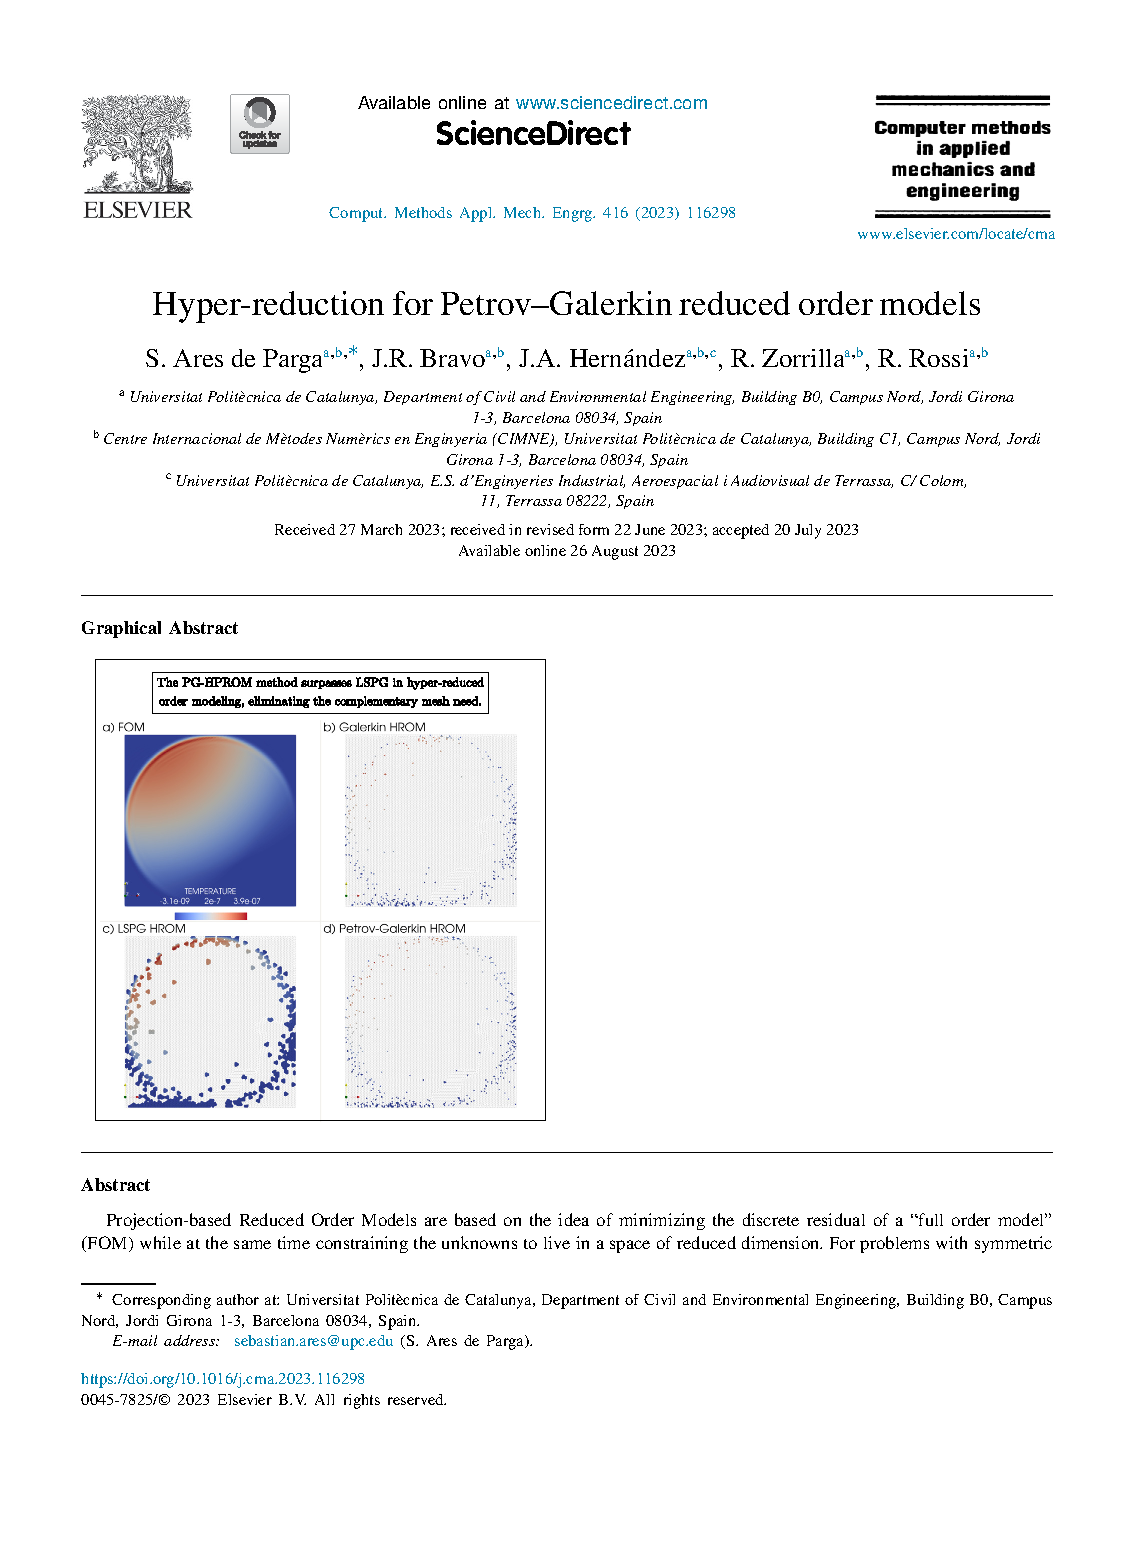
\includepdf[
  pages=-,
  pagecommand={},
  scale=0.92,
  delta=0 0,
  offset=32pt 0pt,
  turn=false
]{Papers/Hyper-reduction_for_Petrov–Galerkin_reduced_order_models.pdf}





% % % CHAPTER 5 - Article 2
\chapter{Parallel reduced order modeling for digital twins using high-performance computing workflows (Article 2)}
\label{chap:article2}

\section*{Preface}

This chapter reproduces the peer-reviewed journal article published in \emph{Computers and Structures}~\cite{Ares2024}, which addresses the integration of PROM techniques with HPC workflows for industrial applications. Building on the methodologies introduced in earlier chapters, this work focuses specifically on overcoming the computational bottlenecks that arise during the offline phase of PROM construction when scaling to large, complex systems.

This contribution represents the main intrusive reduced-order modeling outcome developed within the \href{https://www.eflows4hpc.eu/}{eFlows4HPC} framework, as part of a broader European research pathway that also includes the \href{https://cordis.europa.eu/project/id/800898}{ExaQUte} and \href{https://cordis.europa.eu/project/id/946009}{EdgeTwins} projects. These initiatives provided the theoretical and technological foundations for enabling scalable, real-time digital twin applications through a combination of exascale computing, projection-based ROMs, and edge deployment strategies. The results presented here adapt and extend this foundation to a full high-fidelity industrial use case, demonstrating how an intrusive PROM workflow can be embedded within an HPC-enabled pipeline.

The development of this workflow was made possible through close collaboration between CIMNE/UPC, Universitat Politècnica de València (UPV), Siemens, Barcelona Supercomputing Center (BSC), and partners such as Inria (mesh optimization) and SISSA (non-intrusive ROM methodologies).

The chapter is structured around the following main contributions:
\begin{itemize}
    \item The development of a complete HPC-enabled workflow for intrusive PROM construction, including parallelization of training simulations, distributed SVD algorithms, and the partitioned implementation of the ECM hyper-reduction across computational subdomains, facilitating efficient parallel deployment.
    \item The validation of the proposed workflow through a multiphysics case study involving motor thermal dynamics, demonstrating its scalability, performance, and practical applicability for digital twin scenarios.
    \item The demonstration of an end-to-end Workflow-as-a-Service strategy for industrial deployment, combining HPC, cloud, and edge computing environments (e.g., through Functional Mock-Up Units (FMUs)).
\end{itemize}

The overall workflow is illustrated in Figure~\ref{fig:rom_workflow}, which situates the main intrusive pipeline alongside the mesh optimization and non-intrusive developments carried out in parallel within the same framework.

Overall, this chapter shows that under real-world industrial conditions, even highly efficient projection-based methods require HPC resources for the offline training phase, particularly when handling large-scale multiparametric studies, complex physics, and high-dimensional full-order models. By leveraging HPC workflows and integrating expertise from multiple research partners, the PROMs developed here become viable tools for real-time industrial applications, bridging the gap between high-fidelity simulation and scalable digital twin deployment.

\begin{figure}[h!]
  \centering
  \includegraphics[width=0.95\textwidth]{Figures/Workflow.png}
  \caption{Overview of the ROM workflow developed within the eFlows4HPC framework, highlighting the intrusive PROM path, mesh optimization stage (Inria), and non-intrusive ROM developments (SISSA).}
  \label{fig:rom_workflow}
\end{figure}

\includepdf[
  pages=-,
  pagecommand={},
  scale=0.92,
  delta=0 0,
  offset=32pt 0pt,
  turn=false
]{Papers/Parallel_Reduced_Order_Modeling_for_Digital_Twins_using_High_Performance_Computing_Workflows.pdf}



% CHAPTER 6 - Nonlinear Projection-Based ROMs
\chapter{Nonlinear manifold projection-based reduced order models}
\label{chap:nonlinear_prom}

%Alternative
While linear reduced-order models have proven effective in a range of problems with smooth and low-dimensional solution manifolds, they face critical limitations in regimes dominated by transport phenomena, shock formation, and nonlinear interactions. As seen in the parametric one-dimensional Burgers' problem studied previously, even the most robust linear projections, such as LSPG, struggle to achieve accurate approximations without requiring a prohibitively large number of modes. This behavior reflects the well-known limitations imposed by the Kolmogorov $n$-width barrier~\cite{Quarteroni2014, pinkus2012n}, which restricts the compressibility of the solution manifold and ultimately the efficiency of any linear approximation.

To overcome this bottleneck, nonlinear PMOR has emerged as a powerful alternative. This broader class of methods has demonstrated strong potential in various applications, including structural dynamics~\cite{he2020situ}, compressible and hypersonic CFD~\cite{chmiel2025unified}, and turbulent wake flows~\cite{barnett2022quadratic}, among others.

A diverse set of nonlinear PMOR strategies has been proposed in the literature. Piecewise-affine approximations~\cite{amsallem2012nonlinear, grimberg2021mesh} exploit local linearity and have shown real-time performance in RANS simulations and LES-based fighter jet models. Registration-based techniques~\cite{taddei2020registration, mirhoseini2022model} offer a powerful framework for transport-dominated problems, introducing mesh motion to align dominant features across parameter configurations. Quadratic approximation manifolds~\cite{jain2017quadratic, barnett2022quadratic} offer a simulation-free or data-driven approach with demonstrable improvements in both accuracy and efficiency. Additionally, convolutional autoencoder-based models~\cite{lee2020model, romor2023non} leverage deep neural architectures to learn structured, low-dimensional manifolds directly from high-dimensional flow data, enabling expressive yet compact representations for complex nonlinear dynamics. While these deep learning-based methods effectively address the Kolmogorov $n$-width barrier, their scalability to full-scale industrial problems, particularly those involving high-resolution meshes with millions of degrees of freedom, remains limited and largely untested. This challenge has motivated hybrid strategies such as POD-DL-ROM~\cite{FRESCA2022114181}, which combine POD-based compression with neural decoders to mitigate computational overhead while retaining nonlinear expressivity.


A particularly promising direction is the intrusive latent-space closure modeling framework introduced in~\cite{barnett2023neural} and mathematically analyzed in~\cite{cohen2023nonlinear}, which augments the classical affine approximation by modeling its closure error using a nonlinear map in latent space. This methodology, implemented via PROM-ANN, has demonstrated state-of-the-art performance in large-scale CFD applications, including problems with millions of degrees of freedom, delivering online acceleration by up to three orders of magnitude while maintaining high accuracy, even at reduced dimensions as low as $n = 2$~\cite{chmiel2025unified}. However, these deep learning approaches often suffer from non-interpretability and require substantial training data, which limits their theoretical grounding and practical usability in data-scarce regimes.

To address these challenges, this thesis contributes to recent advances in interpretable, data-efficient, and physics-consistent nonlinear map constructions for reduced-order modeling. In particular, it explores two complementary research directions that target the limitations of nonlinear latent-space closure models: first, the introduction of a discrete physics-informed training strategy for PROM-ANN~\cite{sibuet2025discrete}, which augments standard snapshot-based training with a residual-based loss derived from the underlying finite element formulation; and second, the development of interpretable kernel-based latent-space closure models, namely PROM-GPR and PROM-RBF~\cite{de2025nonlinear}, which replace the neural network with Gaussian process regression (GPR) or radial basis function (RBF) interpolation. Both strategies preserve the latent-space correction structure while enhancing either the physical consistency or the theoretical interpretability of the resulting manifold PROMs.

This chapter does not develop these extensions in full; instead, it serves as a unified conceptual and methodological survey that establishes the context for these advancements. By reviewing the progression from global linear subspace approximations to more expressive nonlinear manifold formulations, culminating in latent-space closure modeling, this chapter situates the motivation for the methodological improvements and alternatives presented in the subsequent chapters. In doing so, it clarifies how overcoming the Kolmogorov $n$-width barrier through nonlinear manifold constructions can significantly improve the efficiency of reduced-order models, and why exploring the incorporation of physical insight into the training process may offer additional benefits in terms of stability, interpretability, or generalization.

A comprehensive formulation, implementation, and validation of the discrete physics-informed training for PROM-ANN is presented in Chapter~\ref{chap:article3}, while the PROM-GPR and PROM-RBF approaches are developed and analyzed in depth in Chapter~\ref{chap:article4}. The remainder of this chapter therefore focuses on situating these contributions within the broader landscape of nonlinear PMOR, using the one-dimensional Burgers' problem as a representative test case to illustrate the strengths and limitations of different manifold-based strategies.




\section{Minimum-residual projection on nonlinear manifolds}
\label{subsec:minres-manifold-rom}

Let us recall the fully discrete set of governing equations derived in the previous chapters, written in terms of a residual operator \( \mathbf{R}: \mathbb{R}^{N} \times [0, T] \times \mathcal{D} \rightarrow \mathbb{R}^{N} \), as
\begin{equation}
\mathbf{R}(\mathbf{u}(t, \boldsymbol{\mu}); t, \boldsymbol{\mu}) = \mathbf{0},
\label{eq:residual_discrete_manifold}
\end{equation}
where \( \mathbf{u}(t, \boldsymbol{\mu}) \in \mathbb{R}^{N} \) denotes the high-fidelity solution at time \( t \in [0, T] \) and for parameter configuration \( \boldsymbol{\mu} \in \mathcal{D} \subset \mathbb{R}^p \).

As discussed in Chapter~\ref{chap:article1}, solving this high-dimensional nonlinear system at each time step and for each parameter configuration can be computationally expensive. 
There, the solution $\mathbf{u}(t,\boldsymbol{\mu})$ was approximated using a linear subspace projection, and the corresponding residual was minimized in a weighted norm. 
To extend this strategy, a general approximation manifold is now considered by expressing the solution through a general decoder function:
\begin{equation}
\mathbf{u}(t,\boldsymbol{\mu}) \;\approx\; \mathbf{\tilde{u}}(t,\boldsymbol{\mu}) 
= \mathbf{u}_{\text{ref}} + D_u(\mathbf{q}(t,\boldsymbol{\mu})),
\label{eq:general_decoder}
\end{equation}
where $\mathbf{u}_{\text{ref}} \in \mathbb{R}^N$ is a chosen reference state, 
$D_u : \mathbb{R}^{n} \rightarrow \mathbb{R}^{N}$ is a general decoder, 
and $\mathbf{q}(t,\boldsymbol{\mu}) \in \mathbb{R}^{n}$ denotes the reduced generalized coordinates. 
An encoder $E_u : \mathbb{R}^{N} \rightarrow \mathbb{R}^{n}$ may also be defined, satisfying $\mathbf{q}(t,\boldsymbol{\mu}) = E_u(\mathbf{u}(t,\boldsymbol{\mu}))$. 
In the linear PROM of Chapter~\ref{chap:linear_prom}, this general formulation reduces to the affine approximation 
$\tilde{\mathbf{u}} = \mathbf{u}_{\text{ref}} + \boldsymbol{\Phi}\mathbf{q}$, which in practice is taken with $\mathbf{u}_{\text{ref}}=0$, 
so that $D_u(\mathbf{q}) = \boldsymbol{\Phi}\mathbf{q}$ and the encoder corresponds to the orthogonal projection $E_u(\mathbf{u}) = \boldsymbol{\Phi}^T \mathbf{u}$. 
For notational simplicity, the following derivations will assume $\mathbf{u}_{\text{ref}}=0$.

The nonlinear encoder–decoder structure associated with this general manifold approximation is illustrated in Figure~\ref{fig:nonlinear_manifold_encoder_decoder}.
\begin{figure}[ht!]
    \centering
    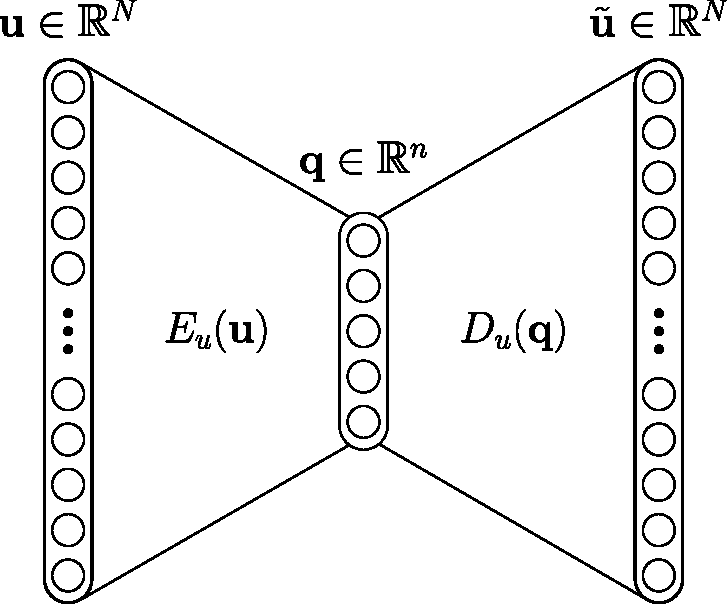
\includegraphics[width=0.5\textwidth]{Figures/nonlinear_manifold_encoder_decoder.pdf}
    \caption{
    Schematic representation of the nonlinear manifold reduction and reconstruction process.
    The high-dimensional state \( \mathbf{u} \in \mathbb{R}^{N} \) is encoded as latent coordinates \( \mathbf{q} \in \mathbb{R}^{n} \) via a nonlinear encoder \( E_u(\mathbf{u}) \), 
    and the approximation \( \tilde{\mathbf{u}} = D_u(\mathbf{q}) \) is reconstructed through a nonlinear decoder \( D_u \). 
    The linear PROM of Chapter~\ref{chap:linear_prom} is recovered as the special case \(D_u(\mathbf{q})=\boldsymbol{\Phi}\mathbf{q}\) with encoder \(E_u(\mathbf{u})=\boldsymbol{\Phi}^T\mathbf{u}\).
    }
    \label{fig:nonlinear_manifold_encoder_decoder}
\end{figure}

Substituting \eqref{eq:general_decoder} into the residual \eqref{eq:residual_discrete_manifold} (with $\mathbf{u}_{\text{ref}}=0$ for simplicity) yields a residual defined on the general approximation manifold:
\begin{equation}
\mathbf{R}(D_u(\mathbf{q}(t, \boldsymbol{\mu}));\,t,\boldsymbol{\mu}).
\end{equation}



Following the residual minimization formulation established for linear subspace PROMs in Chapters~\ref{chap:linear_prom} and ~\ref{chap:article1}, the projection problem is generalized to arbitrary decoders by solving
\begin{equation}
\min_{\mathbf{q}(t, \boldsymbol{\mu}) \in \mathbb{R}^{n}} 
\; \frac{1}{2} \left\lVert 
\mathbf{R}(D_u(\mathbf{q}(t, \boldsymbol{\mu})); t, \boldsymbol{\mu}) 
\right\rVert_{\mathbf{G}}^2,
\label{eq:nonlinear_projection_minimization}
\end{equation}
where \( \|\cdot\|_{\mathbf{G}} \) denotes a norm induced by a symmetric positive definite (SPD) matrix \( \mathbf{G} \in \mathbb{R}^{N \times N} \) (i.e. \( \|\mathbf{v}\|_{\mathbf{G}}^{2} := \mathbf{v}^{T}\mathbf{G}\mathbf{v} \)). This minimization problem extends the optimality conditions from linear PROMs to general approximation manifolds.

\textbf{Notation.} To avoid cumbersome expressions, explicit dependences on \(t\), \(\boldsymbol{\mu}\), and \(\mathbf{q}\) will be omitted after the next equations; unless stated otherwise, all quantities should be understood as functions of \(t\), \(\boldsymbol{\mu}\), and the current reduced state. These dependencies may be reintroduced later in the chapter where appropriate.

The first-order optimality condition associated with \eqref{eq:nonlinear_projection_minimization} leads to the nonlinear system:
\begin{equation}
\left[
\frac{\partial \mathbf{R}}{\partial \mathbf{u}} 
\frac{\partial D_u}{\partial \mathbf{q}}
\right]^T
\mathbf{G} \, 
\mathbf{R} = \mathbf{0},
\end{equation}
which can be expressed in terms of the Jacobian of the residual as:
\begin{equation}
\left[
\mathbf{J} 
\frac{\partial D_u}{\partial \mathbf{q}}
\right]^T
\mathbf{G} \, 
\mathbf{R} = \mathbf{0},
\end{equation}
where \( \mathbf{J} := \tfrac{\partial \mathbf{R}}{\partial \mathbf{u}} \in \mathbb{R}^{N \times N} \).

This projected residual admits an interpretation as a generalized encoder of the residual:
\begin{equation}
E_r(\mathbf{R}) := 
\left(\frac{\partial D_u}{\partial \mathbf{q}}\right)^T 
\mathbf{J}^T 
\mathbf{G} \, \mathbf{R},
\label{eq:general_residual_encoder}
\end{equation}
yielding the reduced residual equation:
\begin{equation}
\mathbf{r}(\mathbf{q}) := E_r\left(\mathbf{R}\right) = \mathbf{0}.
\end{equation}


This nonlinear system in reduced coordinates is solved using a Newton-type iteration:
\begin{equation}
\frac{\partial \mathbf{r}}{\partial \mathbf{q}}^{(k)} \, \delta \mathbf{q}^{(k)} = -\,\mathbf{r}^{(k)},
\end{equation}
which expands to:
\begin{equation}
\left(
\frac{\partial D_u}{\partial \mathbf{q}}
\right)^{(k)T}
\!\!\mathbf{J}^T 
\mathbf{G} 
\mathbf{J}
\left(
\frac{\partial D_u}{\partial \mathbf{q}}
\right)^{(k)} \delta \mathbf{q}^{(k)}
= -
\left(
\frac{\partial D_u}{\partial \mathbf{q}}
\right)^{(k) T}
\!\!\mathbf{J}^T 
\mathbf{G} 
\mathbf{R}^{(k)}.
\label{eq:general_manifold_update}
\end{equation}



Equation~\eqref{eq:general_manifold_update} defines the reduced-order model on a general approximation manifold specified by the decoder \( D_u \), and generalizes the minimum-residual projection framework developed in Chapters~\ref{chap:linear_prom} and ~\ref{chap:article1}. A detailed derivation of this reduced system, including the assumptions involved in the Newton approximation, is provided in Appendix~\ref{app:gauss_newton_manifold}.

\paragraph{Galerkin projection.} 
The Galerkin projection is particularly effective when the Jacobian \( \mathbf{J} \) is SPD. In such cases, setting \( \mathbf{G} = \mathbf{J}^{-T} \) in the minimum-residual condition yields optimal search directions. Substituting this choice into the reduced system \eqref{eq:general_manifold_update} leads to the Galerkin form:
\begin{equation}
\left( \frac{\partial D_u}{\partial \mathbf{q}} \right)^T 
\mathbf{J} 
\left( \frac{\partial D_u}{\partial \mathbf{q}} \right) \delta \mathbf{q} 
= - \left( \frac{\partial D_u}{\partial \mathbf{q}} \right)^T \mathbf{R}.
\label{eq:prom_general_galerkin}
\end{equation}

\paragraph{Least-Squares Petrov–Galerkin (LSPG) projection.} 
In nonlinear problems, the Jacobian \( \mathbf{J} \) is generally not SPD. To address this, the LSPG method adopts \( \mathbf{G} = \mathbf{I} \), ensuring that the reduced model retains the minimum-residual property, which is essential for accuracy and stability. The resulting system becomes:
\begin{equation}
\left( \frac{\partial D_u}{\partial \mathbf{q}} \right)^T 
\mathbf{J}^T 
\mathbf{J} 
\left( \frac{\partial D_u}{\partial \mathbf{q}} \right) \delta \mathbf{q} 
= - \left( \frac{\partial D_u}{\partial \mathbf{q}} \right)^T \mathbf{J}^T \mathbf{R}.
\label{eq:prom_general_lspg}
\end{equation}

\paragraph{}
The preceding formulation establishes a unified framework for projection-based ROMs on general approximation manifolds, encompassing both the Galerkin and LSPG variants as particular cases defined by the choice of the weighting matrix \( \mathbf{G} \). For the remainder of this chapter, the LSPG formulation will be adopted as the standard projection strategy, owing to its improved robustness in convection-dominated systems.

As previously shown in Section~\ref{subsec:galerkin_lspg_comparison}, the one-dimensional inviscid Burgers’ equation was used to illustrate the shortcomings of Galerkin projection in convection-dominated regimes and the stabilizing effect of LSPG. That section also examined key factors such as the construction of the POD basis, the decay of singular values, and the influence of the Kolmogorov \( n \)-width on linear ROM performance.

These findings now serve as a starting point for exploring strategies to overcome the limitations of linear subspace models. Using the same Burgers model problem as a representative testbed, the following sections examine nonlinear ROMs defined on expressive approximation manifolds, aiming to mitigate the Kolmogorov barrier and improve representational accuracy under strong nonlinearity.

\section{Piecewise-linear manifolds via local POD}
The linear subspace approximation underlying classical projection-based ROMs, as discussed in Chapter~\ref{chap:linear_prom}, relies on constructing a global basis \( \boldsymbol{\Phi} \in \mathbb{R}^{N \times n} \) that optimally captures the solution manifold in the least-squares sense. While this approach is effective for smooth or weakly nonlinear problems, it faces severe limitations in transport-dominated regimes (such as the one-dimensional inviscid Burgers' equation examined earlier). In that case, achieving acceptable accuracy required a large number of global modes \( n \), reflecting a large Kolmogorov \( n \)-width and the inability of a single global linear subspace to capture sharp gradients and localized features across the parameter domain and time.

One natural strategy to mitigate this limitation is to abandon the idea of a single global basis and instead adopt \emph{local linear approximations}. This is the principle behind piecewise-linear manifolds and Local POD methods~\cite{amsallem2012nonlinear, grimberg2021mesh}, which partition the solution space into regions where local bases provide more accurate and compact representations. By constructing multiple local bases \( \{ \boldsymbol{\Phi}_i \} \), each tailored to a specific region of the trajectory or parameter space, these methods can better resolve complex solution features with fewer modes per local basis. This local structure effectively lowers the approximation barrier imposed by the global Kolmogorov \( n \)-width and leads to more efficient reduced-order models.

Beyond their conceptual simplicity, piecewise-linear approaches have demonstrated remarkable success in large-scale applications such as transonic aerodynamics and unsteady turbulent flows~\cite{washabaugh2016use, grimberg2021mesh}, delivering real-time or near-real-time performance even in high-dimensional problems with \( N > 10^7 \) degrees of freedom. In the context of the Burgers' model problem considered here, they provide an ideal test case to illustrate how localized bases can significantly improve approximation accuracy.

\subsection{Local subspace construction, clustering, and online basis selection}

To overcome the inherent limitations of global linear subspaces, local POD partitions the solution manifold into smaller regions, each characterized by its own local linear basis tailored specifically to the dynamics of that region.

 The construction described in the following paragraphs, based on clustering in a reduced coordinate space and local POD basis generation, is not unique and does not represent the main methodological contribution of this thesis. It is provided here as a representative formulation to illustrate the key steps involved in building piecewise-linear manifold approximations. A version of this approach was employed in the collaborative work~\cite{bravo2024subspace}.


The local approximation at each time $t$ and parameter configuration $\boldsymbol{\mu}$ is expressed as:
\begin{equation}
\mathbf{u}(t,\boldsymbol{\mu}) \approx \mathbf{\tilde{u}}(t,\boldsymbol{\mu}) 
= \mathbf{u}_{\text{ref},c} + \boldsymbol{\Phi}_c \, \mathbf{q}_c(t,\boldsymbol{\mu}), 
\quad c = 1, \dotsc, N_{\text{local}},
\label{eq:local_pod_approximation}
\end{equation}
where $\mathbf{u}_{\text{ref},c} \in \mathbb{R}^{N}$ denotes the reference state for cluster $c$, 
$\boldsymbol{\Phi}_c \in \mathbb{R}^{N\times n_c}$ is the local POD basis of cluster $c$, 
and $\mathbf{q}_c(t,\boldsymbol{\mu}) \in \mathbb{R}^{n_c}$ are the corresponding local reduced coordinates. 
For notational simplicity, the following derivations will assume $\mathbf{u}_{\text{ref},c}=0$.




\paragraph{Global basis and clustering strategy} 
A global basis \(\boldsymbol{\Phi}_{g}\) is initially constructed by applying POD (via SVD) to the entire snapshot set \(\mathbf{S}\in\mathbb{R}^{N\times N_s}\):
\begin{equation}
\mathbf{S} = \boldsymbol{\Phi}_{g}\,\boldsymbol{\Sigma}_{g}\,\mathbf{V}_{g}^T,
\label{eq:global_svd}
\end{equation}
where \(\boldsymbol{\Phi}_{g}\in\mathbb{R}^{N\times n_g}\) contains the first \(n_g\) global POD modes retained based on a prescribed energy tolerance.

The snapshots are projected onto this global basis to obtain a lower-dimensional representation:
\begin{equation}
\mathbf{q}_{g} = \boldsymbol{\Phi}_{g}^T\,\mathbf{S}\in\mathbb{R}^{n_g\times N_s}.
\label{eq:global_projection}
\end{equation}
A clustering algorithm such as k-means is then applied in this reduced-dimensional coordinate space, partitioning the snapshots into \(N_{\text{local}}\) distinct clusters~\cite{amsallem2012nonlinear, hastie2009elements}. This partitioning yields submatrices \(\mathbf{S}_c\) that contain snapshots assigned to each local cluster:
\begin{equation}
\mathbf{S} = [\mathbf{S}_1,\mathbf{S}_2,\dotsc,\mathbf{S}_{N_{\text{local}}}],
\quad \mathbf{S}_c \in \mathbb{R}^{N \times {N_s}_{(c)}},
\label{eq:local_snapshot_partition}
\end{equation}
where \({N_s}_{(c)}\) is the number of snapshots within the cluster \(c\).

\paragraph{Local basis construction}
For each local snapshot subset \(\mathbf{S}_c\), a local POD basis is computed via SVD:
\begin{equation}
\mathbf{S}_c = \boldsymbol{\Phi}_c \, \boldsymbol{\Sigma}_c \, \mathbf{V}_c^T,
\label{eq:local_svd}
\end{equation}
where \(\boldsymbol{\Phi}_c\in\mathbb{R}^{N\times n_c}\) contains the left singular vectors representing local modes. The local basis dimension \(n_c\) is chosen based on a POD energy criterion:
\begin{equation}
\epsilon(n_c) = 1 - \frac{\sum_{i=1}^{n_c}\sigma_{k,i}^{2}}{\sum_{j=1}^{r_c}\sigma_{k,j}^{2}} \leq \epsilon_{\text{tol}},
\label{eq:local_pod_energy}
\end{equation}
with singular values \(\sigma_{k,i}\) ordered in descending magnitude, and \(r_c\) the numerical rank of cluster \(c\).

\paragraph{Overlapping clusters for smooth transitions}
To ensure smooth transitions between neighboring local subspaces, snapshots near cluster boundaries are included in multiple clusters. A threshold distance criterion in the global reduced space defines the overlap~\cite{Washabaugh2012}. Specifically, snapshots satisfying
\[
\|\mathbf{q}_{g,i} - \mathbf{c}_c\|_2 < \delta_{\text{overlap}},
\]
where \(\mathbf{c}_c\) is the centroid of cluster \(c\), are assigned simultaneously to multiple clusters. The overlapping snapshots between clusters \(c\) and \(c'\) can be denoted as:
\begin{equation}
\mathbf{S}_{\text{overlap}} = [\mathbf{S}_c \cap \mathbf{S}_{k'}],
\end{equation}
where \(\mathbf{S}_{\text{overlap}}\) contains snapshots shared by adjacent clusters. This strategy reduces approximation discontinuities across clusters and improves numerical robustness.


\paragraph{Online local basis selection}
During the online prediction phase, the appropriate local basis for the current state \(\mathbf{u}(t,\boldsymbol{\mu})\) is selected dynamically. First, the state is projected onto the global reduced space:
\begin{equation}
\mathbf{q}_{g}(t,\boldsymbol{\mu}) = \boldsymbol{\Phi}_{g}^T \mathbf{u}(t,\boldsymbol{\mu}).
\end{equation}
Then, the best-fitting local basis is determined via a proximity criterion to the cluster centroids:
\begin{equation}
c^*(t,\boldsymbol{\mu}) = \arg\min_{1\leq c\leq N_{\text{local}}} 
\|\mathbf{q}_{g}(t,\boldsymbol{\mu}) - \mathbf{c}_c\|_2.
\label{eq:online_selection_rule}
\end{equation}

Once the cluster \(c^*\) is identified, the corresponding local encoder–decoder structure is applied:
\begin{equation}
\mathbf{q}_{c^*}(t,\boldsymbol{\mu}) = \boldsymbol{\Phi}_{c^*}^T\,\mathbf{u}(t,\boldsymbol{\mu}),\quad
\mathbf{\tilde{u}}(t,\boldsymbol{\mu}) = \boldsymbol{\Phi}_{c^*}\,\mathbf{q}_{c^*}(t,\boldsymbol{\mu}).
\end{equation}

\paragraph{Local LSPG projection}
Finally, within each selected local subspace, the LSPG projection introduced previously in Section~\ref{subsec:minres-manifold-rom} is employed. The locally projected reduced-order equations are:
\begin{subequations}
\begin{align}
\boldsymbol{\Phi}_{c^*}^T \mathbf{J}^{(k)T} \mathbf{J}^{(k)} \boldsymbol{\Phi}_{c^*} \, \delta \mathbf{q}_{c^*}^{(k)} 
&= - \boldsymbol{\Phi}_{c^*}^T \mathbf{J}^{(k)T} \mathbf{R}^{(k)},
\label{eq:local_lspg_linear}\\
\mathbf{q}_{c^*}^{(k+1)} &= \mathbf{q}_{c^*}^{(k)} + \delta \mathbf{q}_{c^*}^{(k)}.
\label{eq:local_lspg}
\end{align}
\end{subequations}

where \(\mathbf{J}\) is the Jacobian of the full-order residual, \(\mathbf{R}\) is the residual vector, and \(\delta \mathbf{q}_{c^*}^{(i)}\) represents the iterative correction in the reduced coordinates.

\subsection{Illustrative toy example: piecewise-linear manifold on a redundant 3D trajectory}
\label{sec:piecewise_linear}

To illustrate the benefit of piecewise-linear manifold approximations, we adopt a simple parametric toy example inspired by Geelen et al.~\cite{geelen2023operator}.  
The trajectory is defined as:
\[
\mathbf{s}(t) = 
\begin{bmatrix}
\cos(t) \\
\sin(t) \\
0.5\, \cos(2t)
\end{bmatrix},
\quad t \in [0,\,2\pi],
\]
which describes a closed curve embedded in three dimensions.  
The third component introduces a nonlinear dependency that makes the trajectory redundant in three dimensions yet not exactly confined to any single plane.

\vspace{0.5em}

\noindent
\textbf{Global linear manifold approximation.}  
A standard POD is applied to the entire trajectory, producing a single global rank-2 basis.  
This yields a global linear manifold (a plane) that best approximates the data in a least-squares sense but cannot fully capture the redundant local curvature, resulting in a significant approximation error.  
This illustrates the well-known limitations of linear subspace approximations for trajectories with locally varying structure~\cite{geelen2023operator} and is depicted in Figure~\ref{fig:toy_linear_manifold}.

\begin{figure}[ht!]
  \centering
  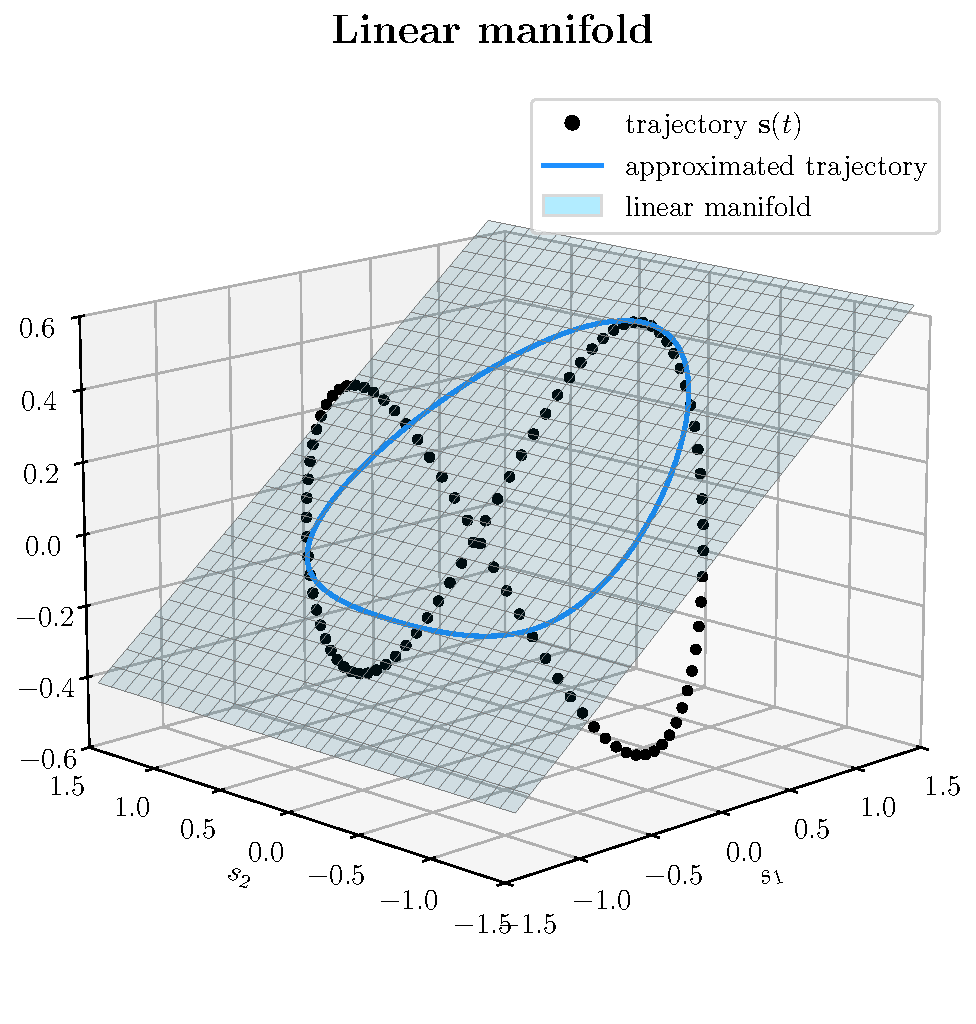
\includegraphics[width=0.45\textwidth]{Figures/linear_manifold.pdf}
  \caption{Global linear manifold (rank-2 plane) approximation of the 3D trajectory. The plane does not fully capture the redundant local curvature.}
  \label{fig:toy_linear_manifold}
\end{figure}

\vspace{0.5em}

\noindent
\textbf{Piecewise-linear manifold approximation.}  
To address this, the trajectory is partitioned into \(N_{\text{local}} = 4\) overlapping segments along the parameter \(t\).  
A local rank-2 POD basis is then constructed for each segment, creating a local linear manifold that best fits that region.  
By blending the local reconstructions in the overlap regions, the piecewise-linear manifold effectively captures the redundant structure and reconstructs the full closed trajectory with negligible error. Figures~\ref{fig:toy_local_manifold1}--\ref{fig:toy_local_manifold4} show each local manifold and its local reconstruction.

\begin{figure}[ht!]
  \centering
  \begin{subfigure}[b]{0.24\textwidth}
    \centering
    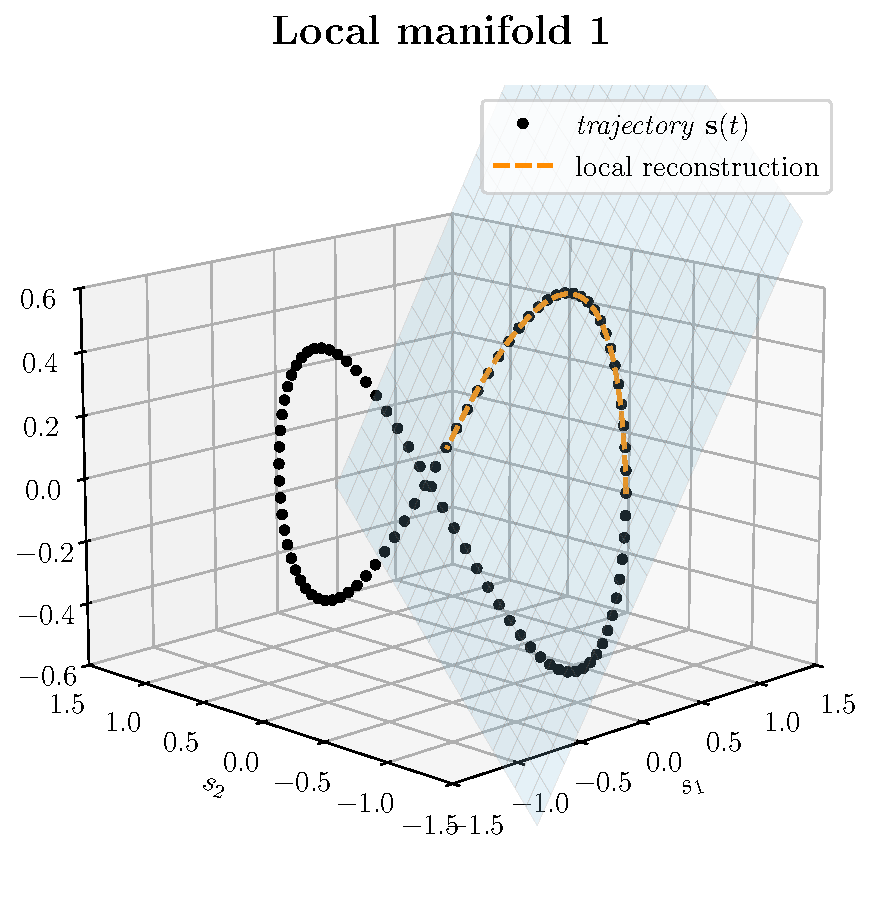
\includegraphics[width=\textwidth]{Figures/local_manifold_1.pdf}
    \caption{Local 1}
    \label{fig:toy_local_manifold1}
  \end{subfigure}
  \hfill
  \begin{subfigure}[b]{0.24\textwidth}
    \centering
    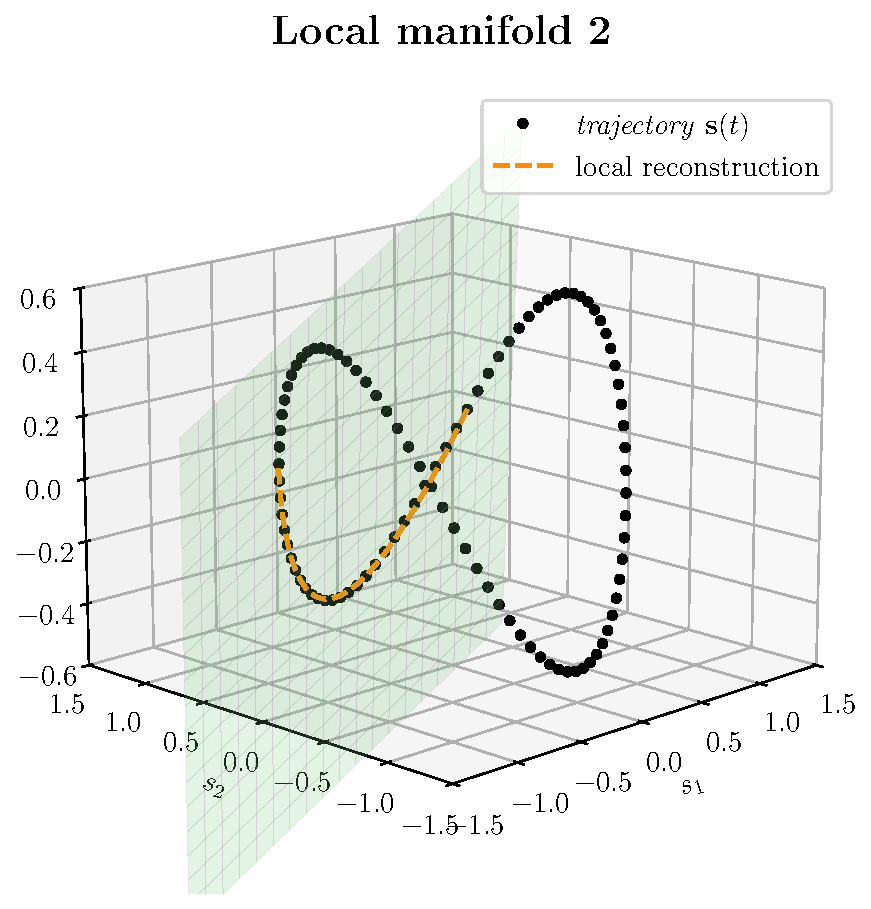
\includegraphics[width=\textwidth]{Figures/local_manifold_2.pdf}
    \caption{Local 2}
    \label{fig:toy_local_manifold2}
  \end{subfigure}
  \hfill
  \begin{subfigure}[b]{0.24\textwidth}
    \centering
    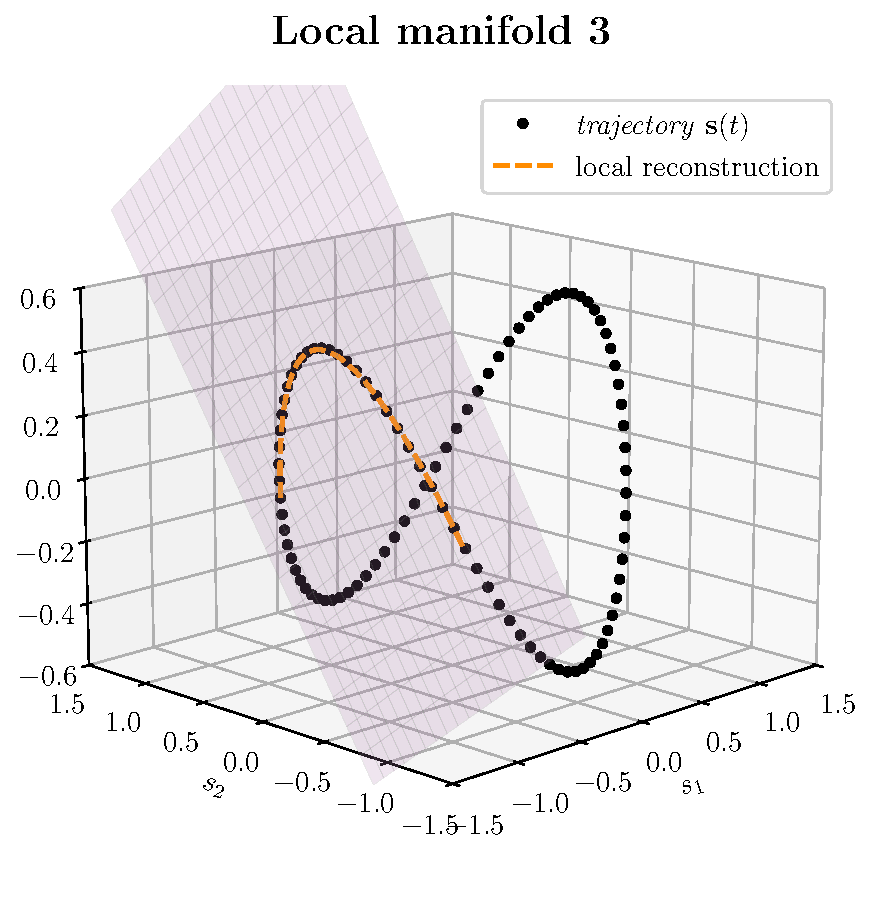
\includegraphics[width=\textwidth]{Figures/local_manifold_3.pdf}
    \caption{Local 3}
    \label{fig:toy_local_manifold3}
  \end{subfigure}
  \hfill
  \begin{subfigure}[b]{0.24\textwidth}
    \centering
    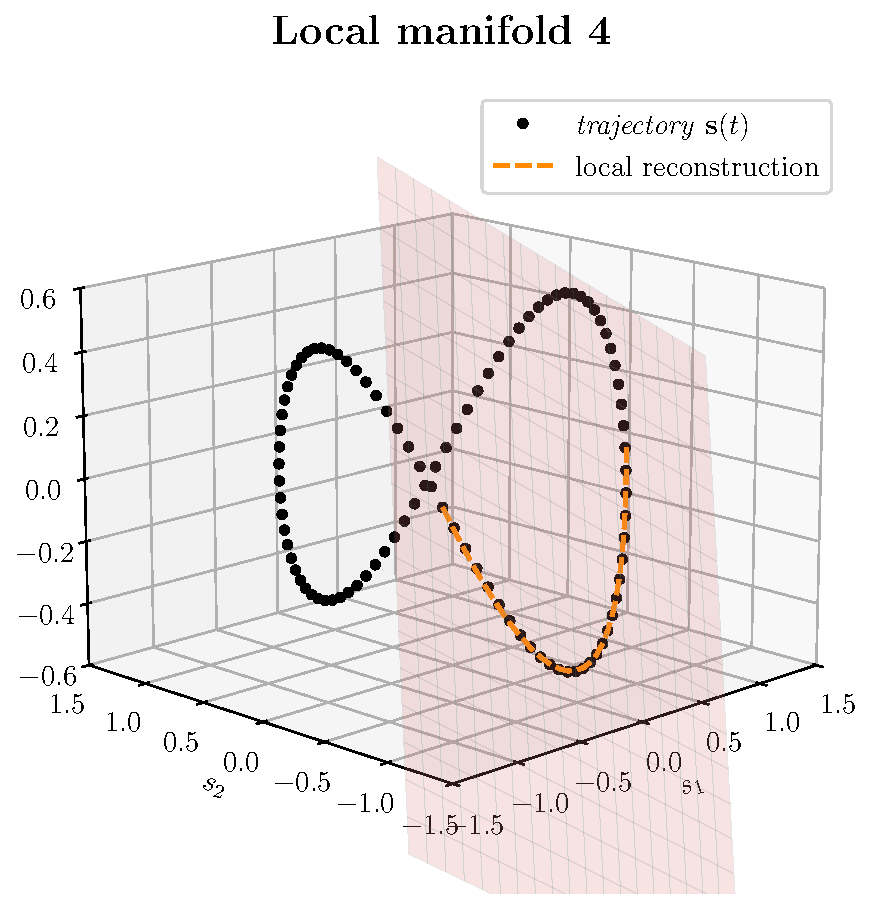
\includegraphics[width=\textwidth]{Figures/local_manifold_4.pdf}
    \caption{Local 4}
    \label{fig:toy_local_manifold4}
  \end{subfigure}

  \caption{Piecewise-local manifold approximations for segments 1--4 (horizontal layout).}
  \label{fig:toy_local_manifolds_all_horizontal}
\end{figure}

Finally, Figure~\ref{fig:toy_piecewise_combined} shows the combined piecewise-linear manifold and the blended approximation, which closely matches the original closed trajectory.  
This simple example highlights how local manifold approaches can overcome the approximation barrier imposed by the Kolmogorov \(n\)-width for problems with local nonlinear features.

\begin{figure}[ht!]
  \centering
  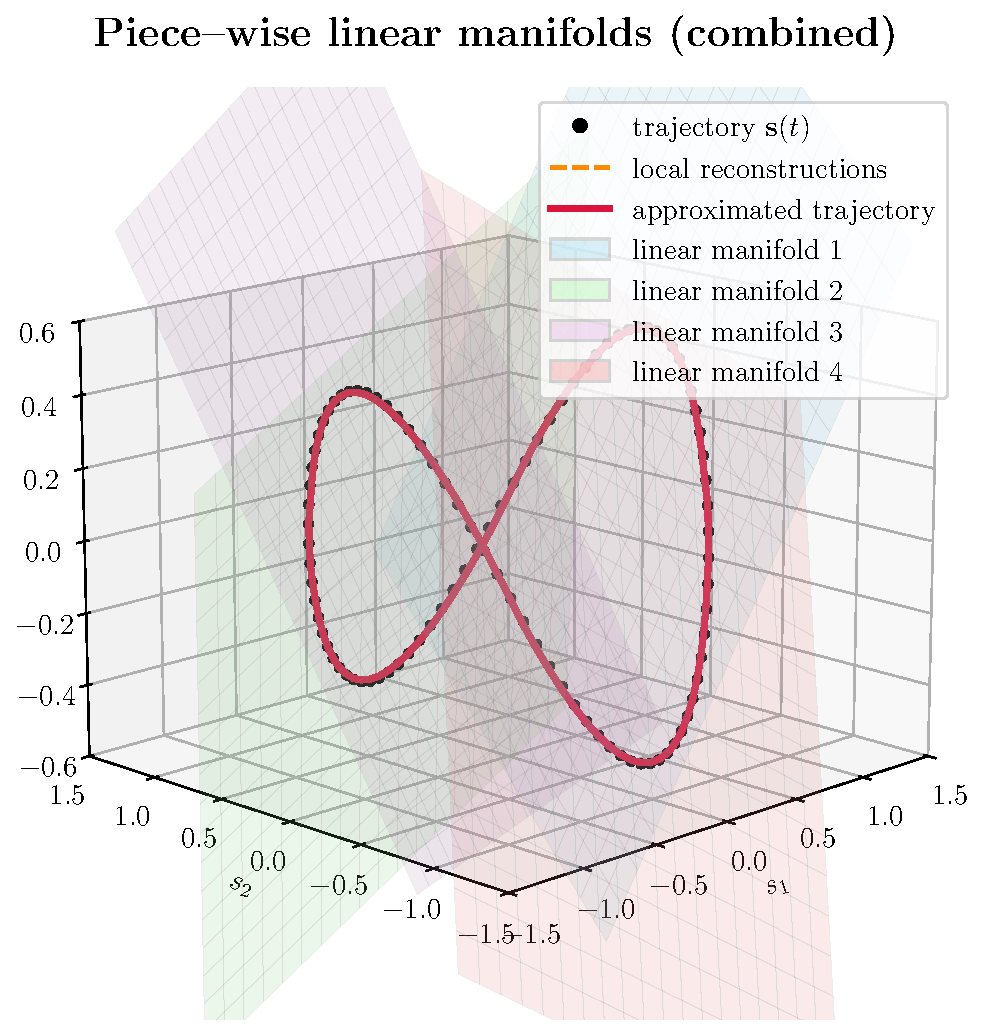
\includegraphics[width=0.45\textwidth]{Figures/piecewise_linear_combined.pdf}
  \caption{Combined piecewise-linear manifold approximation using four local POD bases with overlap. The blended local subspaces collectively recover the full 3D trajectory with minimal error.}
  \label{fig:toy_piecewise_combined}
\end{figure}

\subsection{Local POD PROM for the model problem}

Having established how piecewise-linear manifold approximations can overcome the limitations of a single global linear subspace, we now test this concept on the model problem introduced earlier.  
The inviscid one-dimensional Burgers’ equation, with its sharp gradients and convection-dominated character, provides an ideal setting to evaluate how local bases can reduce the approximation barrier imposed by the Kolmogorov~$n$-width.

In the offline stage, the full-order snapshot matrix is first projected onto a global POD basis, yielding reduced coordinates $\mathbf{q}_{g}$.  
A k-means clustering algorithm partitions these reduced coordinates into distinct clusters, with overlapping assignments to ensure smooth transitions across local bases.  
A local SVD is then performed for each cluster, retaining modes up to a common squared tolerance~$\epsilon^2$.

Figure~\ref{fig:average_modes_clusters} shows how the average number of modes per cluster changes as the number of clusters increases.  
A configuration with 20 clusters and an average of approximately 17.5 modes per cluster was selected, striking a balance between local adaptability and practical offline cost.

\begin{figure}[htbp]
    \centering
    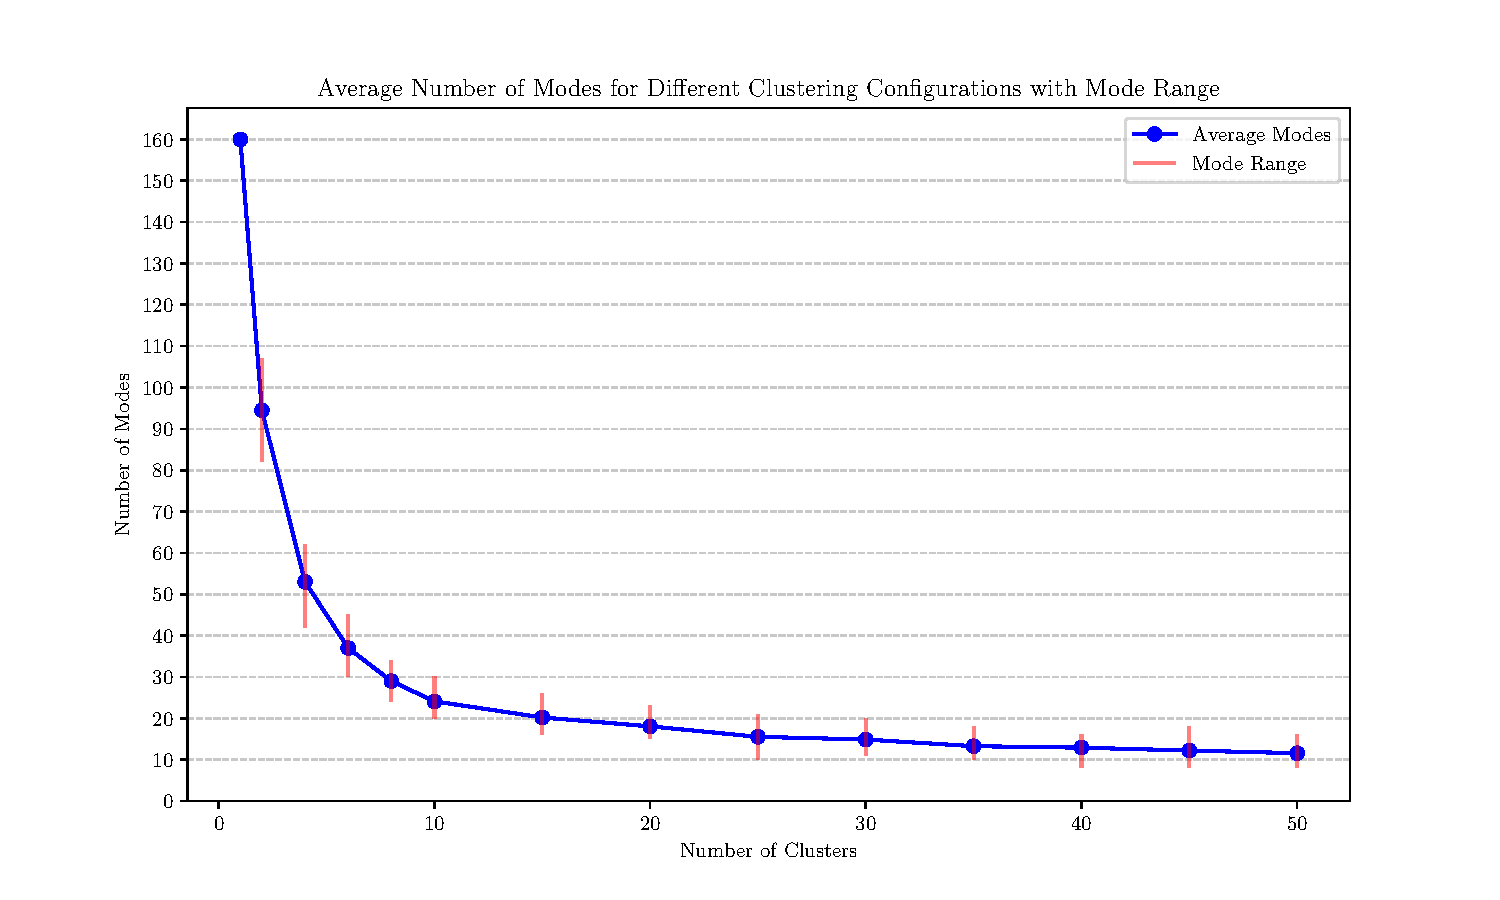
\includegraphics[width=0.7\textwidth]{Figures/average_modes_per_clustering_with_range.pdf}
    \caption{Average number of modes per cluster for different clustering configurations. Vertical bars indicate the range within each setup.}
    \label{fig:average_modes_clusters}
\end{figure}

For illustration, Figure~\ref{fig:fom_vs_local_global_pod} compares the full-order solution with its global and local PROM approximations for a representative parameter point~$\boldsymbol{\mu}_3 = [5.190,\,0.0260]$.  
The local approach visibly improves the resolution of steep wave fronts, demonstrating how local subspace partitioning adapts more effectively to convection-dominated features without requiring a significantly larger reduced dimension.

\begin{figure}[ht!]
    \centering
    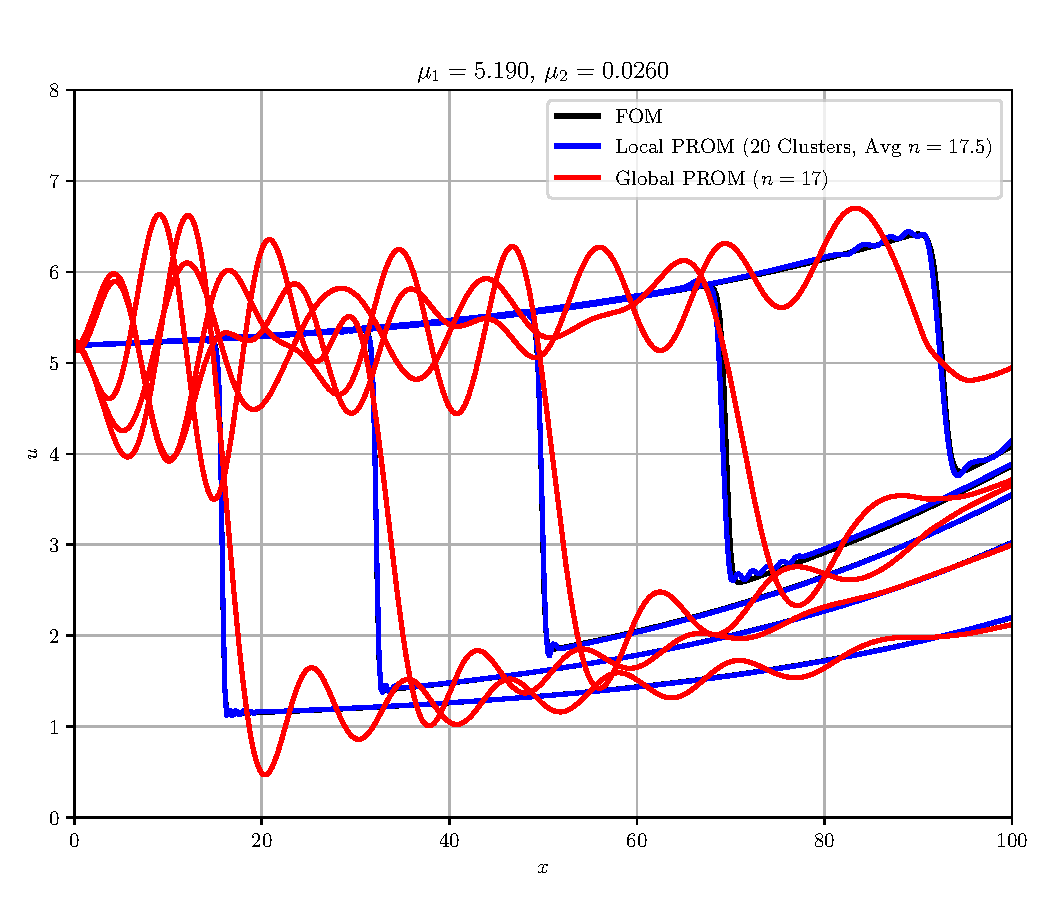
\includegraphics[width=0.7\textwidth]{Figures/fom_local_vs_global_pod_comparison_17_modes.pdf}
    \caption{Comparison of the FOM solution with the global PROM (17 modes) and the local PROM (20 clusters, average 17.5 modes) for $\mu_1 = 5.190$ and $\mu_2 = 0.0260$.}
    \label{fig:fom_vs_local_global_pod}
\end{figure}

Table~\ref{tab:local_global_pod_error_summary} summarizes the maximum relative $L_2$ error computed across three representative test configurations.  
The local PROM consistently achieves a substantial reduction in the worst-case error compared to the global basis while maintaining the same approximate basis size.

\begin{table}[htbp]
    \centering
    \begin{tabular}{c c c}
        \toprule
        Computational model & $n$ & $\mathbb{RE}^{\textbf{max}}_{2, \mathbf{u}}$ (\%) \\
        \midrule
        Global PROM & 17 & 13.52 \\
        Local PROM (20 Clusters) & 17.5 & 1.63 \\
        \bottomrule
    \end{tabular}
    \caption{Relative $L_2$ error across three test configurations for the global and local PROMs (LSPG). Maximum values across the points $\boldsymbol{\mu}_1 = [4.75,\, 0.0200]$, $\boldsymbol{\mu}_2 = [4.56,\, 0.0190]$, and $\boldsymbol{\mu}_3 = [5.19,\, 0.0260]$ are shown.}
    \label{tab:local_global_pod_error_summary}
\end{table}

\begin{table}[htbp]
\centering
\begin{tabular}{l c c}
    \toprule
        Computational model & $n$ & $\mathbb{RE}^{\textbf{max}}_{2, \mathbf{u}}$ (\%) \\
        \midrule
        Global PROM & 17 & 13.52 \\
        Local PROM (20 Clusters) & 17.5 & 1.63 \\
        \bottomrule
\end{tabular}

\medskip
{\small
Relative $L_2$ errors for the three test cases comparing the global and local PROMs.
}
\end{table}


These results confirm that piecewise-linear local PROMs offer a compelling and practical alternative to a single global subspace, especially for convection-dominated and transport problems where the Kolmogorov $n$-width is inherently large. While clustering, overlap, and online basis selection introduce additional offline complexity, these aspects remain manageable and justified by the improved accuracy and stability that local Petrov--Galerkin projections provide. From the hyper-reduction perspective, the local framework integrates well with ECSW-type methods~\cite{grimberg2021mesh}, which rigorously construct element-wise sampling sets through a convex formulation with minimal tuning parameters. This approach supports either a single reduced mesh shared by all local bases, or multiple reduced meshes adapted to each subspace, providing flexibility in balancing accuracy and online cost.

\textbf{As an additional contribution, I co-authored a related work~\cite{bravo2024subspace}} that proposes a novel subspace-adaptive weights cubature method, building on the ECM framework. This extension enables multiple local bases to share a common reduced mesh with tailored weights for each subspace. The resulting approach provides a robust third option for local hyper-reduction and demonstrates scalable performance for highly nonlinear problems, further reinforcing the practicality of local PROMs in large-scale applications.

% \section{Autoencoder-based nonlinear manifolds}

\section{Quadratic manifolds}

Quadratic approximation manifolds have emerged as a promising strategy for overcoming the limitations imposed by the Kolmogorov $n$-width barrier by extending the traditional affine approximation with explicit quadratic terms in the reduced coordinates. These models introduce controlled curvature into the solution representation, enabling more compact and accurate reduced-order models. Early developments in this area include simulation-free formulations for nonlinear structural dynamics problems~\cite{jain2017quadratic}, as well as fully data-driven versions tailored to large-scale CFD applications with transport phenomena~\cite{barnett2022quadratic}. 

Notably, the integration of quadratic approximation manifolds with robust projection and hyper-reduction frameworks, such as the LSPG projection~\cite{carlberg2011efficient} and energy-conserving sampling and weighting (ECSW)~\cite{grimberg2021mesh}, has demonstrated substantial speed-ups and high accuracy for challenging benchmarks like the Ahmed body turbulent wake~\cite{barnett2022quadratic} and hypersonic flow predictions~\cite{chmiel2025unified}. These results illustrate the potential of quadratic manifolds to deliver orders-of-magnitude performance improvements compared to conventional affine PROMs while remaining interpretable, simulation-driven, and relatively data-efficient.

In the following sections, we formalize the general quadratic manifold decoder, derive its associated minimum-residual projection, and present a representative toy example that highlights its ability to capture nonlinear solution features that lie beyond the reach of linear subspaces. Finally, the approach is evaluated for the one-dimensional inviscid Burgers’ equation, providing a consistent comparison to the linear and piecewise-linear strategies discussed earlier.

\subsection{Quadratic manifold formulation}
\label{sec:quad_manifold_formulation}

The quadratic manifold extends the traditional linear subspace approximation by enriching the solution representation with second-order terms in the reduced coordinates. Specifically, the quadratic approximation (decoder) is defined as:
%
\begin{equation}
\tilde{\mathbf{u}}(t,\boldsymbol{\mu}) =
\mathbf{u}_{\text{ref}} +
\boldsymbol{\Phi}\,\mathbf{q}(t,\boldsymbol{\mu}) +
\mathbf{H}\,\bigl(\mathbf{q}(t,\boldsymbol{\mu})\otimes\mathbf{q}(t,\boldsymbol{\mu})\bigr),
\quad
\boldsymbol{\Phi}\in\mathbb{R}^{N\times n},\;
\mathbf{H}\in\mathbb{R}^{N\times n^{2}},
\label{eq:quad_decoder_full}
\end{equation}
%
where $\mathbf{u}_{\text{ref}}\in\mathbb{R}^{N}$ is a chosen reference state (e.g., mean flow or steady-state solution), 
$\boldsymbol{\Phi}$ is the linear POD basis, and $\mathbf{H}$ is a second-order tensor reshaped as a matrix. For notational simplicity, the following derivations will assume $\mathbf{u}_{\text{ref}}=0$ and will omit explicit dependence on $t$ and $\boldsymbol{\mu}$, unless required for clarity.
The term $\mathbf{q}\otimes\mathbf{q}\in\mathbb{R}^{n^{2}}$ denotes the full Kronecker product, explicitly containing all quadratic monomials:
%
\[
\mathbf{q}\otimes\mathbf{q}=
\begin{bmatrix}
q_1^2,\,q_1 q_2,\,\dots,\,q_1 q_n,\,
q_2 q_1,\,q_2^2,\,\dots,\,q_n^2
\end{bmatrix}^T.
\]

However, this representation introduces redundancy since cross-terms such as \(q_i q_j\) and \(q_j q_i\) appear twice. To remove this redundancy, we employ the symmetric quadratic monomial vector:
%
\begin{equation}
\mathbf{Q}_s(\mathbf{q}) =
\begin{bmatrix}
q_1^{2},\, q_1 q_2,\, q_1 q_3,\, \dots,\, q_2^2,\,\dots,\,q_n^{2}
\end{bmatrix}^{T}\in\mathbb{R}^{k}, \quad k=\frac{n(n+1)}{2}.
\label{eq:symmetric_monomials}
\end{equation}

With this symmetric representation, the quadratic decoder becomes:
%
\begin{equation}
D_u(\mathbf{q}) =
\boldsymbol{\Phi}\mathbf{q} +
\mathbf{H}_s\,\mathbf{Q}_s(\mathbf{q}),
\quad \mathbf{H}_s\in\mathbb{R}^{N\times k}.
\label{eq:quad_decoder_sym}
\end{equation}

\paragraph{Practical selection of the latent dimension.}
Given a POD energy tolerance $\epsilon$ and a padding factor $\zeta$, 
we first compute the smallest integer $n_{\text{tra}}$ such that the leading
$n_{\text{tra}}$ singular values capture at least $(1-\epsilon)$ of the
snapshot energy.  
Since a quadratic manifold with $n$ primary coordinates contains
$k=\tfrac{n(n+1)}{2}$ distinct quadratic monomials, we choose the minimal $n$
satisfying $k \ge n_{\text{tra}}$ and then inflate it by the factor
$(1+\zeta)$ to provide headroom for additional variance.  
Finally, an upper bound 
$
n \le n_{\max}=\frac{\sqrt{1+8N_s}-1}{2}
$
is enforced so that the symmetric-Kronecker matrix has at least as many rows
as snapshots, keeping the ridge-regression system well posed.


\textbf{Offline construction of the quadratic manifold} The quadratic manifold is constructed from the available snapshot set by determining the linear basis \(\boldsymbol{\Phi}\) and the quadratic coefficient tensor \(\mathbf{H}_s\). For each of the \(N_s\) snapshots, we first define the linear reconstruction errors:
%
\[
\mathbf{e}_\ell =
\mathbf{u}_\ell - \boldsymbol{\Phi}\mathbf{q}_\ell,
\quad \ell=1,\dots,N_s,
\]
%
which are collected into the error matrix:
%
\[
\mathbf{E} =
\begin{bmatrix}
\mathbf{e}_1 & \dots & \mathbf{e}_m
\end{bmatrix}\in\mathbb{R}^{N\times N_s}.
\]

To identify the quadratic terms, we construct a symmetric quadratic regression matrix:
%
\[
\mathbf{Z} =
\begin{bmatrix}
\mathbf{Q}_s(\mathbf{q}_1) & \dots & \mathbf{Q}_s(\mathbf{q}_m)
\end{bmatrix}\in\mathbb{R}^{k\times N_s},
\]
%
where each column \(\mathbf{Q}_s(\mathbf{q}_\ell)\) contains the unique quadratic monomials defined in \eqref{eq:symmetric_monomials} evaluated at \(\mathbf{q}_\ell\).

The quadratic coefficient tensor \(\mathbf{H}_s\) is determined by solving the regularized least-squares (ridge regression) problem:
%
\[
\min_{\mathbf{H}_s}\|\mathbf{E}-\mathbf{H}_s\mathbf{Z}\|_F^2+\alpha^2\|\mathbf{H}_s\|_F^2,
\]
%
where \(\alpha>0\) is the Tikhonov regularization parameter. This problem admits a closed-form solution obtained via the thin SVD \(\mathbf{Z}= \mathbf{U}_z\boldsymbol{\Sigma}_z\mathbf{V}_z^T\):
%
\begin{equation}
\mathbf{H}_s=
(\mathbf{U}_z\operatorname{diag}(f))
\left(\mathbf{V}_z^T\mathbf{E}^T/\boldsymbol{\Sigma}_z\right)^T,
\quad
f_\ell=\frac{\sigma_\ell^2}{\sigma_\ell^2+\alpha^2},\, \ell=1,\dots,r.
\label{eq:H_closedform}
\end{equation}

Here, the division by \(\boldsymbol{\Sigma}_z\) denotes element-wise division by each singular value.

\textbf{Derivative of the quadratic decoder} The derivative of the quadratic decoder \eqref{eq:quad_decoder_full} with respect to the reduced coordinates \(\mathbf{q}\) in the full Kronecker form is initially expressed as:
%
\begin{equation}
\frac{\partial\tilde{\mathbf{u}}}{\partial\mathbf{q}}(\mathbf{q}) =
\boldsymbol{\Phi} +
\mathbf{H}\left[\mathbf{q}\otimes\mathbf{I}+\mathbf{I}\otimes\mathbf{q}\right],
\label{eq:quad_derivative_full}
\end{equation}
%
with \(\mathbf{I}\) the \(n\times n\) identity.

However, employing the symmetric quadratic monomial vector \(\mathbf{Q}_s(\mathbf{q})\), the derivative simplifies to a compact form directly suitable for efficient computation:
%
\begin{equation}
\frac{\partial D_u}{\partial\mathbf{q}} =
\boldsymbol{\Phi} +
\mathbf{H}_s\,\frac{\partial\mathbf{Q}_s}{\partial\mathbf{q}},
\quad
\frac{\partial\mathbf{Q}_s}{\partial\mathbf{q}}\in\mathbb{R}^{k\times n}.
\label{eq:quad_derivative_sym}
\end{equation}

Each row of the matrix \(\partial\mathbf{Q}_s/\partial\mathbf{q}\) is derived analytically as follows:

\begin{itemize}
    \item Diagonal terms: \(\displaystyle\frac{\partial(q_i^2)}{\partial q_i}=2q_i.\)
    \item Off-diagonal terms (\(j>i\)): 
    \(\displaystyle\frac{\partial(q_i q_j)}{\partial q_i}=q_j,\quad \frac{\partial(q_i q_j)}{\partial q_j}=q_i.\)
\end{itemize}

\paragraph{LSPG minimum-residual projection on quadratic manifolds}

The quadratic manifold PROM (QPROM) adopts the same minimum-residual projection framework introduced in Section~\ref{subsec:minres-manifold-rom}. At each online time step, the reduced coordinates are updated via a Gauss--Newton iteration that solves:
\begin{equation}
\Bigl(\frac{\partial D_u}{\partial\mathbf{q}}\Bigr)^{(k)T} 
\mathbf{J}^{(k)T} \mathbf{J}^{(k)}
\Bigl(\frac{\partial D_u}{\partial\mathbf{q}}\Bigr)^{(k)}
\,\delta\mathbf{q}^{(k)}
= 
-\Bigl(\frac{\partial D_u}{\partial\mathbf{q}}\Bigr)^{(k)T}
\mathbf{J}^{(k)T}\mathbf{R}^{(k)},
\label{eq:lspg_quad_proj}
\end{equation}
where the decoder derivative $\partial D_u/\partial \mathbf{q}$ follows its definition in Eq.~\eqref{eq:quad_derivative_sym}. This ensures a consistent and robust minimum-residual projection for quadratic manifold approximations.


\subsection{Illustrative toy example: quadratic manifold on a redundant 3D trajectory}

We revisit the illustrative example of Section~\ref{sec:piecewise_linear}, employing a quadratic manifold approximation instead of a piecewise-linear one. The trajectory \(\mathbf{s}(t)\) remains the same, embedding a closed curve in three-dimensional space with a nonlinear dependency that prevents accurate representation by a single linear subspace. First, a global rank-2 POD basis is obtained from the snapshot data as before. Rather than partitioning the manifold, we enrich this global linear representation by introducing quadratic terms, resulting in a single curved manifold (a paraboloid). Figure~\ref{fig:toy_quadratic_manifold} shows the resulting quadratic manifold, clearly demonstrating its improved capacity to represent the original trajectory without the need for multiple local bases.

\begin{figure}[ht!]
  \centering
  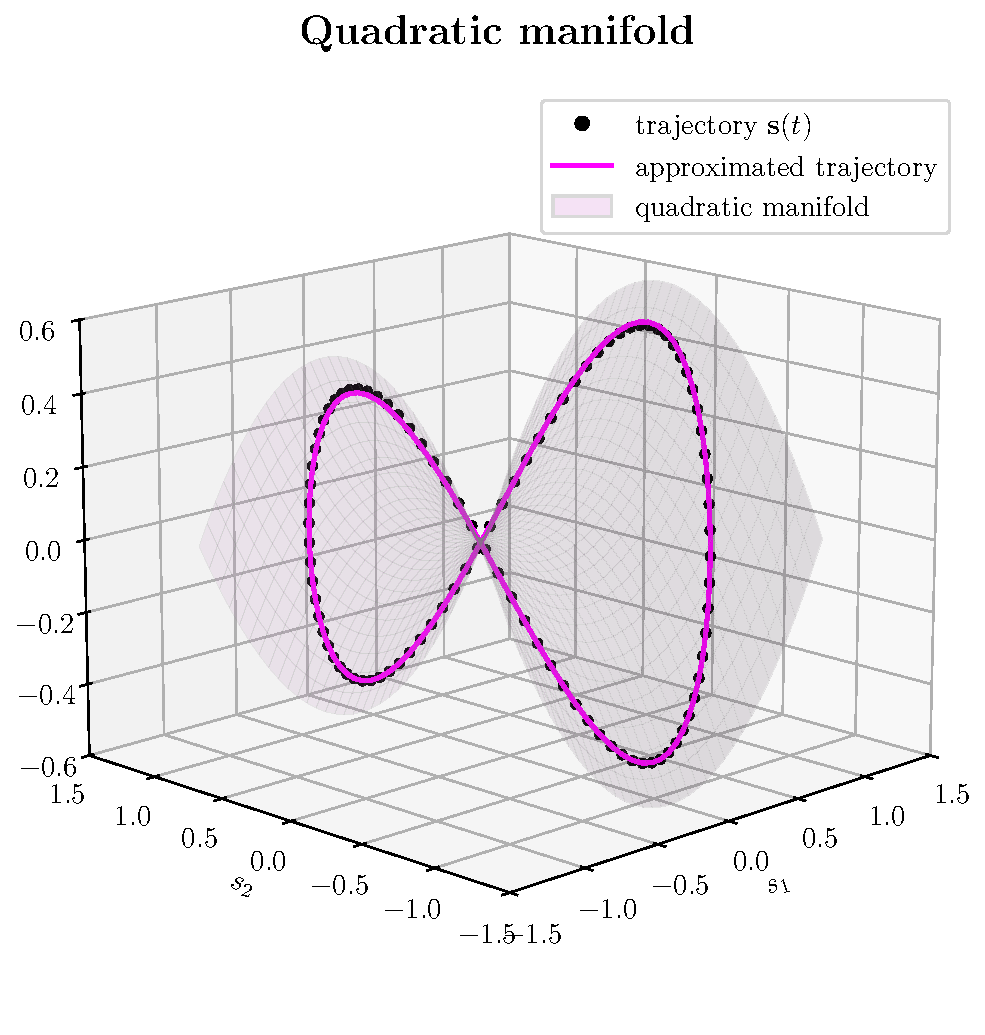
\includegraphics[width=0.6\textwidth]{Figures/quadratic_manifold.pdf}
  \caption{Quadratic manifold approximation of the 3D trajectory. By enriching the global linear subspace with quadratic terms, the manifold accurately captures the local curvature inherent in the trajectory.}
  \label{fig:toy_quadratic_manifold}
\end{figure}

Compared to the linear manifold approximation, the quadratic manifold achieves a significantly reduced approximation error due to its intrinsic ability to represent nonlinear solution structures. This simple yet illustrative example highlights the power of quadratic manifold approximations in overcoming the limitations imposed by the Kolmogorov \(n\)-width barrier, without the complexity associated with piecewise or local constructions.


\subsection{Quadratic manifold PROM for the model problem}

Having demonstrated the potential of quadratic manifold approximations to represent nonlinear solution features efficiently, we now evaluate this approach on the one-dimensional inviscid Burgers’ equation introduced previously as the model problem. The convection-dominated character and sharp gradients of this test case provide a stringent setting to assess the effectiveness of the quadratic manifold in addressing the limitations associated with global linear subspace approximations.

The offline construction begins by applying POD to the snapshot dataset, yielding a global linear subspace \(\boldsymbol{\Phi}\). The quadratic manifold tensor \(\mathbf{H}_s\) is then identified through regularized regression, following the procedure described in Section~\ref{sec:quad_manifold_formulation}. Using a POD energy tolerance of $\epsilon = 10^{-6}$ and a 10\% padding factor ($\zeta = 0.1$), the automatic dimension-selection procedure described in Section~\ref{sec:quad_manifold_formulation} yields $n = 21$ retained coordinates for the QPROM. This value balances reconstruction accuracy with computational cost while ensuring the quadratic regression system is well posed.


Figure~\ref{fig:fom_vs_quadratic_rom} compares the FOM solution with both the QPROM and a global linear POD PROM for the representative test case \(\boldsymbol{\mu} = [4.750,\,0.0200]\). Clearly, the quadratic manifold approximation significantly improves the resolution of the nonlinear features of the solution, capturing steep gradients and sharp wave fronts more accurately than the linear PROM.

\begin{figure}[htbp]
    \centering
    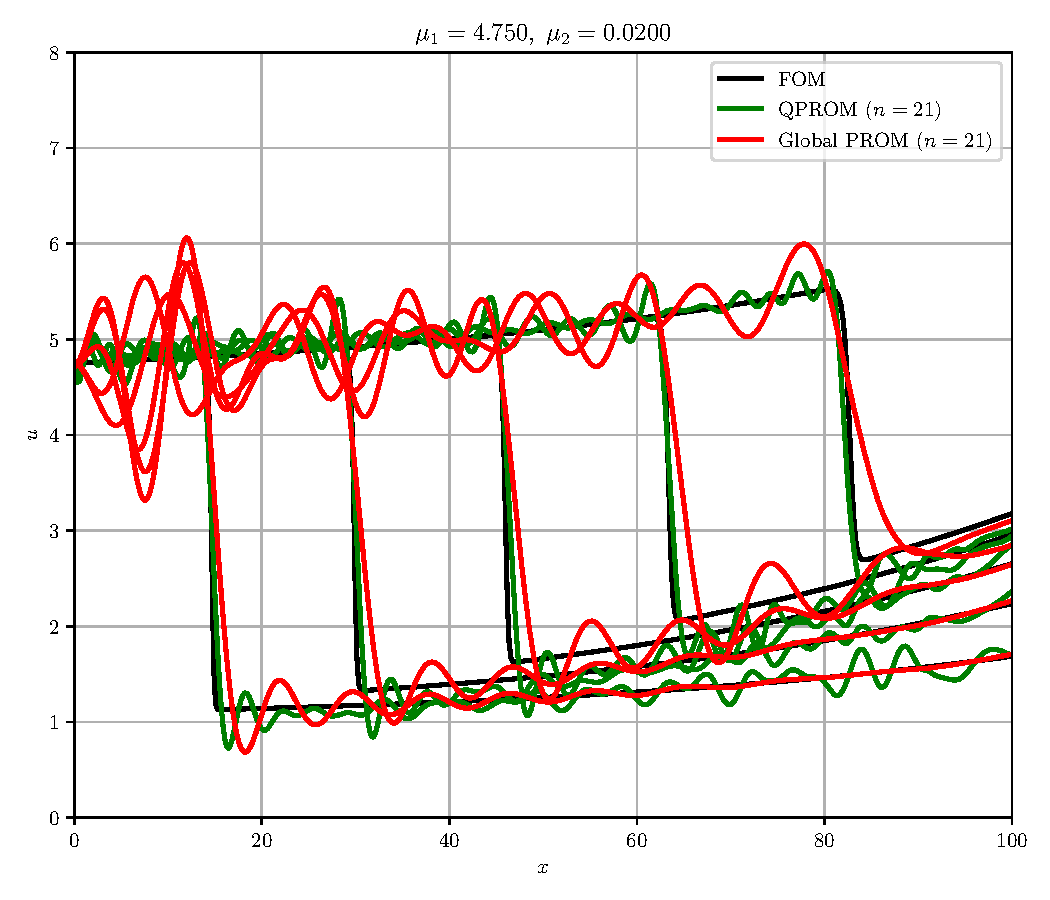
\includegraphics[width=0.7\textwidth]{Figures/fom_vs_qprom_mu1_4.750_mu2_0.0200.pdf}
    \caption{Comparison of the FOM solution with the QPROM (21 modes) and the global linear PROM (21 modes) for the parameter set \(\mu_1 = 4.750\), \(\mu_2 = 0.0200\).}
    \label{fig:fom_vs_quadratic_rom}
\end{figure}

Table~\ref{tab:quad_vs_global_pod_error_summary} summarizes the maximum relative \(L_2\) error computed across three representative test configurations. The quadratic manifold consistently achieves significant error reduction compared to the global linear POD PROM, clearly demonstrating its capability to overcome the approximation barrier posed by the Kolmogorov \(n\)-width with modest computational effort.

\begin{table}[htbp]
    \centering
    \begin{tabular}{c c c}
        \toprule
        Computational Model & $n$ & $\mathbb{RE}^{\textbf{max}}_{2, \mathbf{u}}$ (\%) \\
        \midrule
        Global PROM & 21 & 9.74 \\
        QPROM & 21 & 4.67 \\
        \bottomrule
    \end{tabular}
    \caption{Maximum relative \(L_2\) error computed across the three test parameter sets \(\boldsymbol{\mu}_1 = [4.750,\, 0.0200]\), \(\boldsymbol{\mu}_2 = [4.560,\, 0.0190]\), and \(\boldsymbol{\mu}_3 = [5.190,\, 0.0260]\).}
    \label{tab:quad_vs_global_pod_error_summary}
\end{table}


These results highlight the QPROM as a compelling and practical alternative to global linear subspace approaches. By explicitly introducing controlled nonlinear curvature through quadratic terms, this method substantially reduces approximation errors over purely linear representations, circumventing the dimensional limitations associated with linear subspaces, without introducing the complexity of clustering or local basis selection inherent to local POD methods. Furthermore, the quadratic manifold integrates naturally with hyper-reduction techniques such as ECSW or ECM, facilitating scalable and efficient implementations for large-scale industrial applications~\cite{barnett2022quadratic,chmiel2025unified}.

However, the quadratic manifold approach still has limitations. While its effectiveness is notable for problems exhibiting mild to moderate nonlinearities, highly complex phenomena, such as strong discontinuities, shock-shock interactions, or intricate parametric dependencies, may require even richer representations. In such cases, a single quadratic manifold may be insufficient, and extensions like piecewise quadratic approximations or fully nonlinear latent-space models based on machine learning regressors may be needed. This motivates the exploration of nonlinear latent-space closure modeling approaches in the next section, which aim to combine the robustness of projection-based formulations with the expressivity of modern machine learning architectures. In particular, recent results for the hypersonic double-cone problem~\cite{chmiel2025unified}, featuring shock-shock interactions and multiple nonlinear flow phenomena, demonstrate that, although the quadratic manifold reduces the number of retained modes from 16 to 12 compared to a standard PROM, it is ultimately outperformed by a PROM-ANN~\cite{barnett2023neural, chmiel2025unified} model using only 2 latent variables, achieving superior speed-ups and accuracy.


\section{Nonlinear manifold construction via latent-space closure modeling with neural networks}
\label{sec:latent_nn}

While quadratic manifold approaches provide a structured yet limited means of modeling closure errors by explicitly defining a quadratic dependence on generalized coordinates, a more general strategy is to represent the closure error using flexible, nonlinear functions learned directly from data. In this context, neural-network-based latent-space closure modeling emerges naturally as a powerful extension of previously discussed manifold formulations, particularly effective for problems exhibiting complex nonlinear behaviors, strong convection, or shocks.

Several neural-network-based methods have recently been proposed for constructing nonlinear approximation manifolds. Among them, convolutional autoencoder architectures \cite{lee2020model, romor2023non} represent an influential direction, utilizing deep convolutional neural networks to embed high-dimensional solutions into low-dimensional nonlinear manifolds. Lee and Carlberg \cite{lee2020model} successfully applied deep convolutional autoencoders to dynamical systems, while Romor et al. \cite{romor2023non} combined convolutional autoencoders with a reduced over-collocation method, achieving notable results in fluid dynamics. However, these convolution-based approaches inherently scale poorly with increasing problem dimensionality, restricting their applicability in practice primarily to problems of moderate size, far below the scales encountered in typical industrial models with millions of degrees of freedom.

An alternative nonintrusive strategy that avoids this scalability bottleneck is the POD-DL-ROM framework~\cite{FRESCA2022114181}, which decouples spatial complexity from network training via a deep feedforward network acting on POD-reduced coordinates. While this model has shown promising results in various parametric problems, its fully nonintrusive nature still limits the incorporation of governing physics or residual consistency into the learning process.

Addressing these scalability and physics-integration limitations, Barnett et al.~\cite{barnett2023neural} introduced a novel latent-space closure framework within the PMOR paradigm. Their approach, known as PROM-ANN, utilizes deep ANNs to model the closure errors explicitly within the low-dimensional latent space, directly circumventing the computational burden associated with high-dimensional network training. By training only within the reduced latent coordinates, thus decoupling the training complexity from the dimension of the original HDM, this methodology achieves significant computational advantages and improved scalability. Moreover, unlike nonintrusive models, PROM-ANN preserves the intrusive structure of projection-based ROMs, enabling future extensions that embed physical constraints into the training procedure.


This framework was successfully demonstrated for challenging convection-dominated problems characterized by slow-decaying Kolmogorov $n$-widths, such as unsteady parametric shock-driven flows and hypersonic flow regimes \cite{barnett2023neural, chmiel2025unified}. In particular, Barnett et al.~\cite{barnett2023neural} illustrated the PROM-ANN capability by constructing hyperreduced PROMs (HPROM-ANNs) achieving superior accuracy compared to traditional affine-based HPROMs. Specifically, they demonstrated nearly three orders of magnitude acceleration over the underlying HDM with approximately 97\% accuracy, utilizing dramatically smaller reduced dimensions. Moreover, Chmiel et al.~\cite{chmiel2025unified} successfully extended this method to hypersonic flows governed by the Navier–Stokes equations, highlighting its effectiveness even at extremely low-dimensional manifolds.

This thesis builds directly upon these developments, exploring deeper methodological improvements and alternative strategies aimed at further enhancing performance, robustness, and interpretability of latent-space closure models. The subsequent subsections provide detailed formulation and illustrative examples of ANN-based latent-space closure, setting the stage for the proposed methodological extensions presented in the following chapters.


\subsection{Latent closure model formulation: ANN-based nonlinear manifolds}
\label{subsec:latent_ann_formulation}

As previously discussed, the general manifold projection-based reduced order modeling approach seeks solutions on nonlinear manifolds parametrized by reduced coordinates~$\mathbf{q}(t,\boldsymbol{\mu})$. In the latent-space closure framework~\cite{barnett2023neural, cohen2023nonlinear}, the approximation manifold is constructed by partitioning a global reduced-order basis $\boldsymbol{\Phi}_{\text{tot}}$, obtained via POD and energy truncation, into two orthogonal subspaces:
\begin{equation}
\boldsymbol{\Phi}_{\text{tot}} = [\,\boldsymbol{\Phi},\, \overline{\boldsymbol{\Phi}}\,], 
\quad 
\boldsymbol{\Phi} \in \mathbb{R}^{N \times n}, 
\quad 
\overline{\boldsymbol{\Phi}} \in \mathbb{R}^{N \times \bar{n}},
\quad 
n \ll \bar{n} \ll N.
\label{eq:basis_partition_latent}
\end{equation}
The columns of $\boldsymbol{\Phi}$ define the retained modes explicitly resolved by the PROM, while the columns of $\overline{\boldsymbol{\Phi}}$ correspond to discarded modes, whose influence is modeled nonlinearly. The resulting nonlinear decoder takes the form:
\begin{equation}
\mathbf{u}(t,\boldsymbol{\mu}) \approx \tilde{\mathbf{u}}(t,\boldsymbol{\mu}) 
= D_u(\mathbf{q}(t,\boldsymbol{\mu})) 
= \mathbf{u}_{\text{ref}} + \boldsymbol{\Phi}\,\mathbf{q}(t,\boldsymbol{\mu}) 
+ \overline{\boldsymbol{\Phi}}\,\mathcal{N}(\mathbf{q}(t,\boldsymbol{\mu})),
\label{eq:decoder_latent}
\end{equation}
where $\mathbf{u}_{\text{ref}} \in \mathbb{R}^N$ is a chosen reference state and 
$\mathcal{N}:\mathbb{R}^n\rightarrow\mathbb{R}^{\bar{n}}$ is a nonlinear closure map, in this case, realized by an artificial neural network.

Unless otherwise stated, and for notational simplicity, the following derivations will assume $\mathbf{u}_{\text{ref}}=0$ and will omit explicit dependence on $(t,\boldsymbol{\mu})$.



\paragraph{Construction of the latent-space closure via ANN}
The nonlinear closure map $\mathcal{N}$ can be effectively represented using machine learning regression methods, particularly ANNs. Given the solution snapshots $\{\mathbf{u}_{s}\}_{s=1}^{N_s}$, the primary and secondary generalized coordinates for training are computed by projection onto the partitioned basis:
\begin{equation}
\mathbf{q}_{s} = \boldsymbol{\Phi}^T \mathbf{u}_{s},\quad
\bar{\mathbf{q}}_{s} = \overline{\boldsymbol{\Phi}}^T \mathbf{u}_{s}, 
\quad s = 1,\dots,N_s.
\label{eq:proj_coordinates_ann}
\end{equation}


The ANN approximation of the nonlinear latent map is then trained by minimizing a mean-squared-error loss:
\begin{equation}
\boldsymbol{\eta}^{*} = \arg\min_{\boldsymbol{\eta}} 
\frac{1}{N_{\text{train}}}
\sum_{s=1}^{N_{\text{train}}}
\left\|
\bar{\mathbf{q}}_{s}
-
\mathcal{N}(\mathbf{q}_{s};\,\boldsymbol{\eta})
\right\|_{2}^{2},
\label{eq:ann_training}
\end{equation}
where $\boldsymbol{\eta}$ denotes the ANN parameters. Note that the dimension of this regression problem scales with $n$ and $\bar{n}$, independently of the HDM dimension $N$, ensuring scalability to large-scale models.


\paragraph{LSPG minimum-residual projection on ANN-based nonlinear manifolds}

Given the nonlinear decoder in Eq.~\eqref{eq:decoder_latent}, the LSPG minimum-residual projection follows the general residual minimization framework introduced in Section~\ref{subsec:minres-manifold-rom}. For ANN-based latent-space closures, the Gauss--Newton iteration for the reduced coordinates at each discrete time step reads:
\begin{equation}
\Bigl(\frac{\partial D_u}{\partial \mathbf{q}}\Bigr)^{(k)T} 
\mathbf{J}^{(k)T} \mathbf{J}^{(k)}
\Bigl(\frac{\partial D_u}{\partial \mathbf{q}}\Bigr)^{(k)}
\,\delta\mathbf{q}^{(k)}
= 
-\Bigl(\frac{\partial D_u}{\partial \mathbf{q}}\Bigr)^{(k)T}
\mathbf{J}^{(k)T}\mathbf{R}^{(k)},
\label{eq:lspg_iter_ann}
\end{equation}
where the Jacobian of the nonlinear decoder is given by:
\begin{equation}
\frac{\partial D_u}{\partial\mathbf{q}} 
= \boldsymbol{\Phi} + \overline{\boldsymbol{\Phi}}\,\frac{\partial\mathcal{N}}{\partial\mathbf{q}},
\quad
\text{with} \quad 
\frac{\partial\mathcal{N}}{\partial\mathbf{q}} \text{ evaluated at iteration } (k).
\label{eq:decoder_derivative_ann}
\end{equation}
The term $\partial\mathcal{N}/\partial\mathbf{q}$ is efficiently computed via automatic differentiation or backpropagation.
  



\paragraph{Hyperreduction via ECSW/ECM for latent-space ANN closures}

For practical scalability, compatibility with project--then--approximate hyperreduction methods such as ECSW or ECM is essential. Following this approach, the full residual projection is approximated using a sparse cubature rule over a reduced mesh $\widetilde{\mathcal{E}}$:
\begin{equation}
\tilde{\mathbf{R}}(D_u(\mathbf{q})) 
= \sum_{e \in \widetilde{\mathcal{E}}} 
\xi_{e}\,\mathbf{L}_{e}^{T}\mathbf{R}_{e}\Bigl(\mathbf{L}_{e^{+}}D_u(\mathbf{q})\Bigr),
\end{equation}
where the positive weights $\{\xi_{e}\}$ and the reduced mesh are determined offline by solving a nonnegative least-squares problem:
\begin{equation}
\boldsymbol{\xi}^{*} = \arg\min_{\boldsymbol{\xi} \geq 0} 
\|\mathbf{C}\boldsymbol{\xi} - \mathbf{d}\|_2^2, 
\quad 
\|\mathbf{C}\boldsymbol{\xi} - \mathbf{d}\|_2 
\leq \varepsilon_{\text{tol}}\,\|\mathbf{d}\|_2,
\end{equation}
with rows of $\mathbf{C}$ and $\mathbf{d}$ encoding projected residual contributions from the training snapshots. 

A key step for nonlinear manifold approximations is that the generalized coordinates $\{\mathbf{q}_s\}_{s=1}^{N_s}$ used in the offline training must be recovered by solving a nonlinear manifold inversion for each snapshot:
\begin{equation}
\boldsymbol{\delta}(\mathbf{q}') = \boldsymbol{\Phi}\,\mathbf{q}' + \overline{\boldsymbol{\Phi}}\,\mathcal{N}(\mathbf{q}') - \mathbf{u}_s = \mathbf{0},
\end{equation}
which is typically solved by Gauss--Newton iteration with Moore--Penrose updates. For further details, see~\cite{barnett2023neural}.

\subsection{Illustrative toy example: latent closure on a redundant 3D trajectory}
\label{subsec:latent_ann_toy}

In this toy example, the latent-space closure framework is demonstrated on the same redundant 3D trajectory used in Section~\ref{sec:piecewise_linear}. A global POD basis is computed, yielding two retained modes ($n=2$) and one discarded mode ($\bar{n}=1$). The nonlinear map $\mathcal{N}$ is approximated using a simple feedforward ANN, which learns the relationship between the primary and secondary generalized coordinates.

Figure~\ref{fig:toy_ann_manifold} shows the closed trajectory, the ANN-based reconstruction, and the latent-space nonlinear manifold defined by the decoder in Eq.~\eqref{eq:decoder_latent}. Despite the minimal size of the closure ($\bar{n}=1$), the ANN captures the local curvature that a purely linear basis would miss. 

In practical high-dimensional problems, the number of discarded modes $\bar{n}$ is typically much larger than the toy example shown here, and a more expressive nonlinear mapping is required; this will be demonstrated for the model problem in the following section. This simple illustration highlights the role of latent closure modeling: to enrich the low-dimensional solution representation via a flexible nonlinear map, overcoming the limitations of linear subspaces with minimal additional cost.

\begin{figure}[ht!]
  \centering
  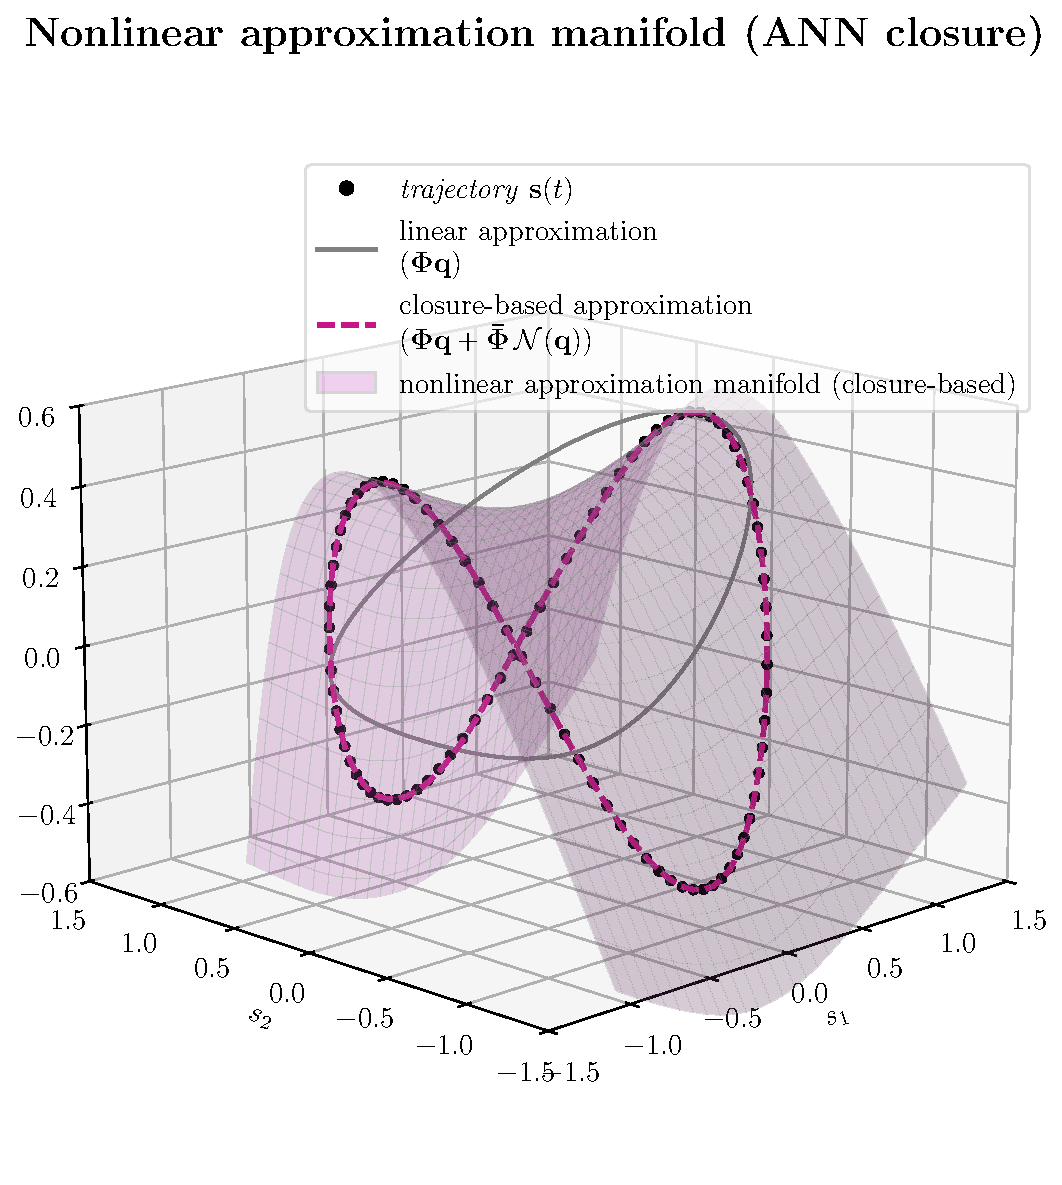
\includegraphics[width=0.6\textwidth]{Figures/nonlinear_closure_manifold_ann.pdf}
  \caption{ANN-based latent-space closure modeling inducing a nonlinear approximation manifold 
for the redundant 3D trajectory. The nonlinear mapping corrects the retained modes to recover 
the full trajectory.}
  \label{fig:toy_ann_manifold}
\end{figure}

\subsection{PROM-ANN with latent-space closure for the model problem}
\label{subsec:latent_ann_model_problem}

The nonlinear latent-space closure framework described in Section~\ref{subsec:latent_ann_formulation} is now tested on the same parametric inviscid Burgers’ problem.
This setup provides an ideal demonstration of how the PROM-ANN architecture can substantially mitigate the Kolmogorov $n$-width barrier by augmenting a minimal set of primary modes with a flexible data-driven correction.

For the offline stage, the full-order snapshots are projected onto a global POD basis and partitioned into retained modes (\(n\)) and discarded modes (\(\bar{n}\)).  
The closure map is constructed using a fully connected feed-forward neural network with five hidden layers and ELU activations, balancing expressiveness with training stability.  
This choice enables the model to learn complex latent relationships efficiently while keeping the regression problem tractable, especially when scaling to high-dimensional industrial meshes.

Figure~\ref{fig:fom_vs_ann_prom_5.19} illustrates the performance of the PROM-ANN at the representative point $\boldsymbol{\mu}_3 = [5.190,\, 0.0260]$ using $n=17$ retained modes and $\bar{n}=79$ discarded modes.
The PROM-ANN approximation significantly improves upon the equivalent global linear POD PROM with the same $n=17$, yielding sharper wavefront resolution and more accurate shock capturing while requiring no local bases or piecewise treatment.
A further comparison with the over-resolved global PROM ($n=96$) shows that the PROM-ANN achieves a competitive level of accuracy with an order-of-magnitude smaller linear subspace.

\begin{figure}[htbp]
    \centering
    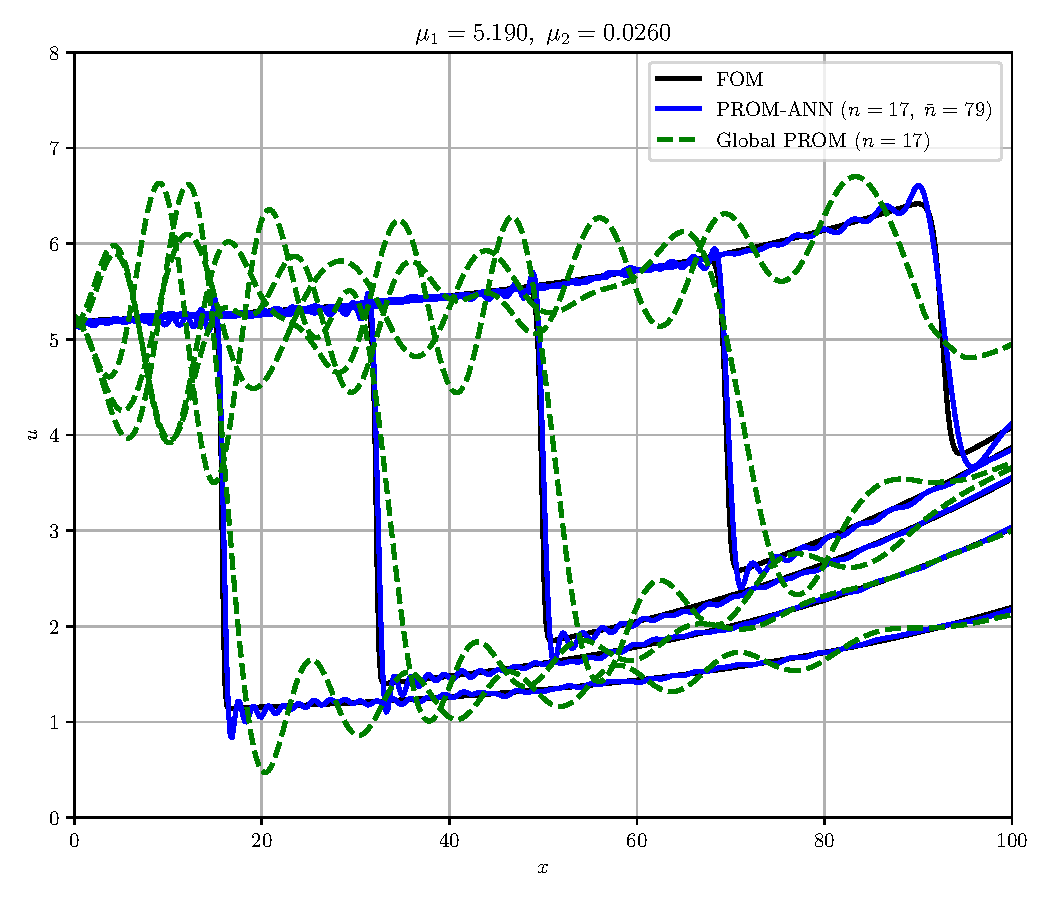
\includegraphics[width=0.49\textwidth]{Figures/fom_vs_ann17_nb79_vs_global17_mu1_5.190_mu2_0.0260.pdf}
    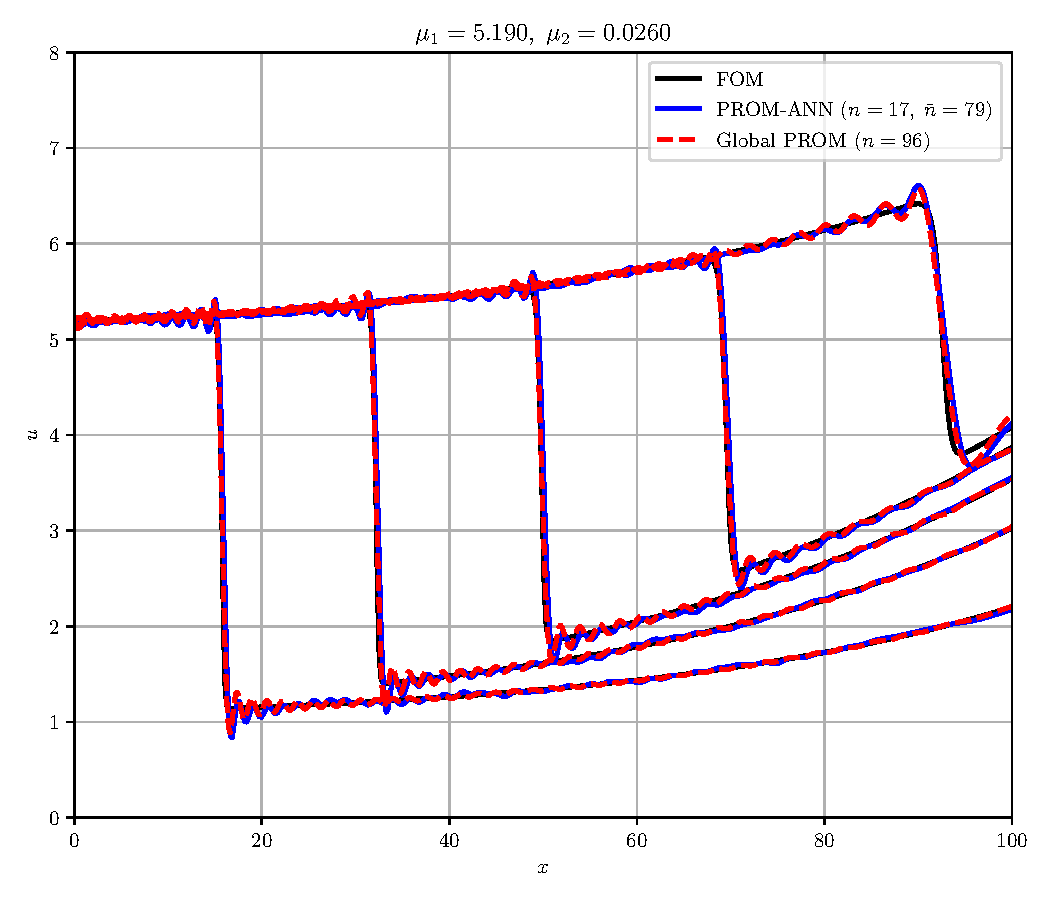
\includegraphics[width=0.49\textwidth]{Figures/fom_vs_ann17_nb79_vs_global96_mu1_5.190_mu2_0.0260.pdf}
    \caption{Comparison of the FOM solution with the PROM-ANN ($n=17$, $\bar{n}=79$) and two global linear POD PROMs ($n=17$ and $n=96$) for $\mu_1 = 5.190$, $\mu_2 = 0.0260$.}
    \label{fig:fom_vs_ann_prom_5.19}
\end{figure}

To further demonstrate the expressive power of the PROM-ANN approach, the retained basis is reduced aggressively to $n=5$, with a corresponding closure space of $\bar{n}=91$.  
Figure~\ref{fig:fom_vs_ann_prom_4.56} shows results at $\boldsymbol{\mu}_2 = [4.560,\, 0.0190]$.  
Despite the drastic dimension reduction, the PROM-ANN preserves a high level of fidelity, dramatically outperforming the global linear PROM with $n=5$ and remaining competitive with the global PROM with $n=96$ modes.

\begin{figure}[htbp]
    \centering
    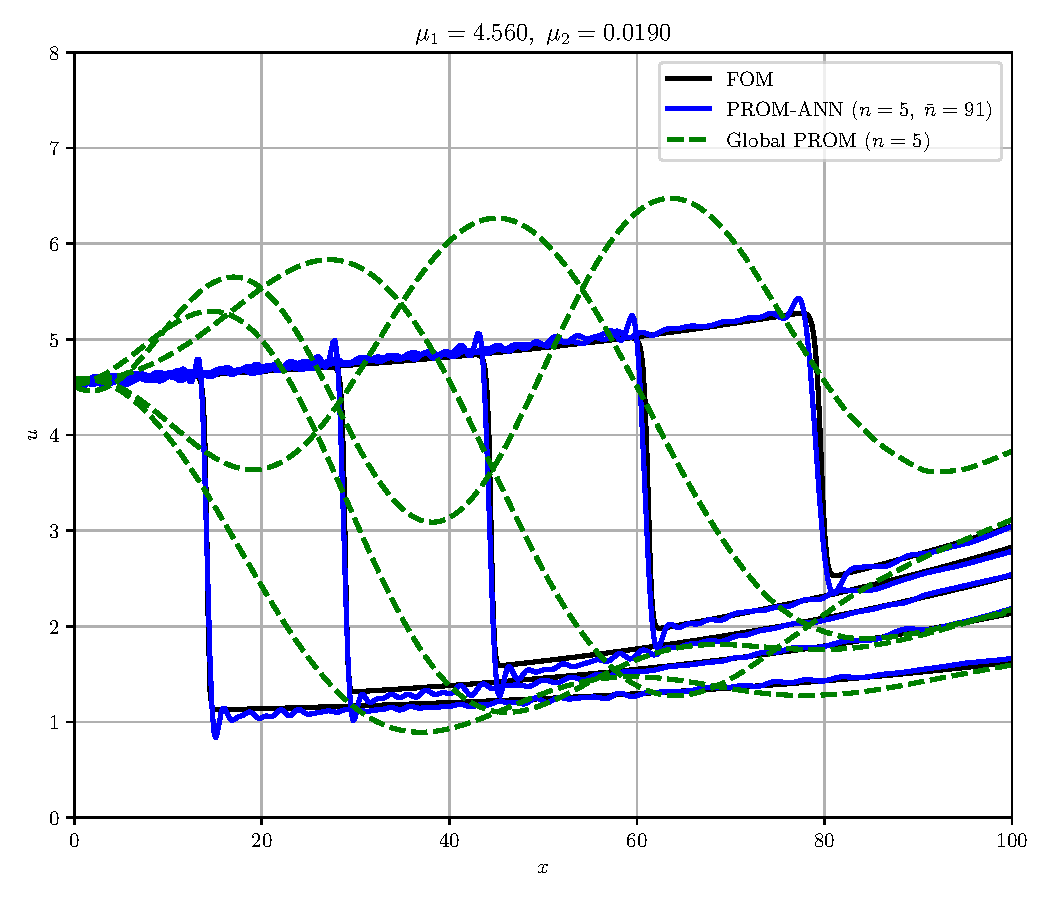
\includegraphics[width=0.49\textwidth]{Figures/fom_vs_ann5_nb91_vs_global5_mu1_4.560_mu2_0.0190.pdf}
    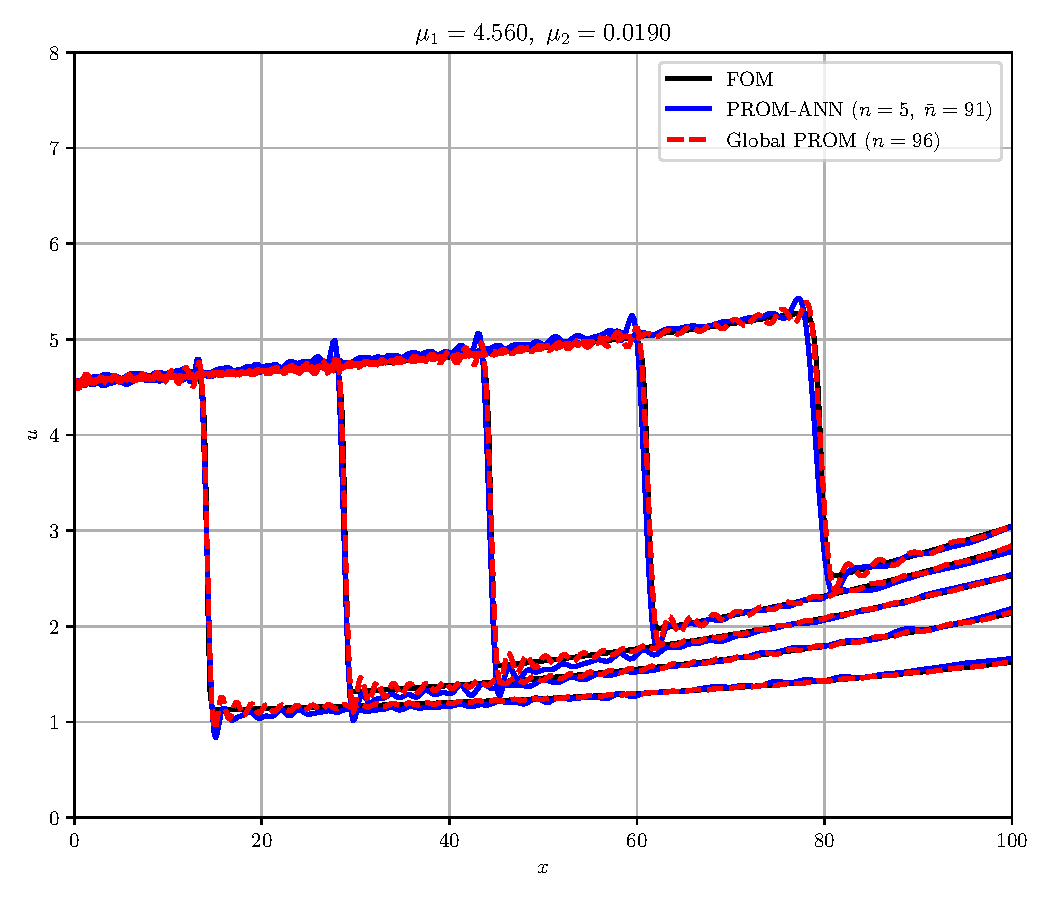
\includegraphics[width=0.49\textwidth]{Figures/fom_vs_ann5_nb91_vs_global96_mu1_4.560_mu2_0.0190.pdf}
    \caption{Comparison of the FOM solution with the PROM-ANN ($n=5$, $\bar{n}=91$) and two global linear POD PROMs ($n=5$ and $n=96$) for $\mu_1 = 4.560$, $\mu_2 = 0.0190$.}
    \label{fig:fom_vs_ann_prom_4.56}
\end{figure}

Table~\ref{tab:prom_ann_error_summary} summarizes the maximum relative $L_2$ errors computed across all three test configurations.
Compared to the best equivalent global linear PROM, the PROM-ANN achieves more than an order-of-magnitude improvement in worst-case error for the aggressively reduced case ($n=5$) and consistently delivers near-optimal accuracy for the moderate basis ($n=17$).

\begin{table}[htbp]
    \centering
    \begin{tabular}{c c c c}
        \toprule
        Computational model & $n$ & $\bar{n}$ & $\mathbb{RE}^{\textbf{max}}_{2, \mathbf{u}}$ (\%) \\
        \midrule
        Global PROM & 17 & - & 13.52 \\
        PROM-ANN & 17 & 79 & 2.40 \\
        \midrule
        Global PROM & 5 & - & 21.23 \\
        PROM-ANN & 5 & 91 & 2.36 \\
        \midrule
        Global PROM & 96 & - & 1.09 \\
        \bottomrule
    \end{tabular}
    \caption{Relative $L_2$ errors for the PROM-ANN and corresponding global linear PROMs across the three test configurations. Maximum values are shown for each setting.}
    \label{tab:prom_ann_error_summary}
\end{table}


These results highlight how latent-space closure modeling with an ANN can push the limits of linear subspace compression in convection-dominated regimes, providing a robust alternative to piecewise or polynomial manifold extensions.
The selected neural network architecture, while simple, demonstrates that even modest latent closures can deliver substantial gains when integrated into a residual-minimizing projection framework.
This flexibility underscores the PROM-ANN’s promise for scalable industrial applications, especially when combined with hyper-reduction strategies to ensure real-time performance.


\section{Towards improvements and alternatives to nonlinear latent-space closure models: discrete physics-informed training and machine learning regression for closure error modeling}
\label{sec:latent_closure_improvements}

The analyses presented in this chapter highlight both the promise and the current limitations of nonlinear manifold PROMs, particularly latent-space closure models. While the PROM-ANN approach demonstrates significant improvements over traditional linear subspace ROMs, especially in convection-dominated regimes, it still inherits key challenges common to data-driven surrogates: limited interpretability, sensitivity to training data availability, and potential inconsistencies with the physics governing the full-order model.

Addressing these aspects suggests methodological enhancements along two complementary directions: introducing \emph{physics-awareness} into the training process and exploring more \emph{transparent regression strategies} for modeling closure errors.

On one hand, ensuring that the learned nonlinear manifold behaves consistently with the governing equations is essential for robust intrusive PROM deployment. Motivated by this need for residual consistency:
\begin{itemize}
    \item \textbf{Chapter~\ref{chap:article3}} presents a discrete physics-informed training approach that augments the standard snapshot loss with a residual-based loss derived directly from the finite element residual. This hybrid training formulation blends data-driven and physics-informed components, explicitly driving the PROM-ANN manifold to represent not only the solution snapshots but also the residual structure that governs the dynamics. As demonstrated in the associated peer-reviewed study, this strategy improves the alignment between offline training and online residual minimization, paving the way for more reliable nonlinear PROMs for strongly nonlinear problems~\cite{sibuet2025discrete}.
\end{itemize}

On the other hand, the reliance on black-box neural networks for closure modeling often complicates interpretability and error certification, especially in data-sparse scenarios. To address this concern:
\begin{itemize}
    \item \textbf{Chapter~\ref{chap:article4}} investigates alternative latent-space closure models based on \emph{Gaussian Process Regression (PROM-GPR)} and \emph{Radial Basis Function interpolation (PROM-RBF)}. Both methods preserve the latent correction structure established in the PROM-ANN framework but replace the deep network with kernel-based surrogates that offer closed-form expressions, tunable hyperparameters, and, in the case of GPR, predictive uncertainty estimates. These regression-based strategies have proven particularly effective for transport-dominated flows and large-scale CFD models, delivering accuracy comparable to PROM-ANN while dramatically reducing data requirements and enhancing theoretical transparency~\cite{de2025nonlinear}.
\end{itemize}

Collectively, these two research directions---physics-informed training and interpretable regression for latent-space closures---form a critical bridge between the foundational PROM-ANN methodology and its practical extension to industrially relevant problems. The next two chapters consolidate these contributions, providing full mathematical derivations, detailed implementation workflows, and extensive validation studies that demonstrate the effectiveness of these advanced nonlinear PROMs.



% \clearpage

% \begin{tabbing}
% \hspace{4cm} \= \kill
% $N$ \> Number of full-order DoFs \\
% $n$ \> Number of retained modes (primary coordinates) \\
% $\bar{n}$ \> Number of discarded modes (closure coordinates) \\
% $N_s$ \> Total number of snapshots available \\
% $N_{\text{train}}$ \> Number of training snapshots for closure model \\
% $N_{\text{local}}$ \> Number of local clusters (piecewise-linear) \\
% $P$ \> Number of parameter samples \\
% $N_t$ \> Number of time steps per parameter \\
% $k$ \> Dimension of symmetric quadratic vector, $k = n(n+1)/2$ \\

% $\mathbf{u}$ \> Full-order state vector \\
% $\tilde{\mathbf{u}}$ \> ROM-reconstructed solution \\
% $\mathbf{u}_{\text{ref}}$ \> Reference state (mean or steady solution) \\
% $\mathbf{q}$ \> Retained reduced coordinates \\
% $\bar{\mathbf{q}}$ \> Latent closure coordinates \\
% $\mathbf{q}_c$ \> Local reduced coordinates (cluster $c$) \\
% $\mathbf{q}_g$ \> Global reduced coordinates for clustering \\
% $\mathbf{c}_c$ \> Cluster centroid \\
% $\delta_{\text{overlap}}$ \> Overlap threshold for clusters \\

% $\boldsymbol{\Phi}$ \> Retained POD basis matrix \\
% $\overline{\boldsymbol{\Phi}}$ \> Discarded POD basis \\
% $\boldsymbol{\Phi}_{\text{tot}}$ \> Total basis before partitioning \\
% $\boldsymbol{\Phi}_c$ \> Local POD basis (cluster $c$) \\
% $\mathbf{H}_s$ \> Quadratic manifold tensor (symmetric) \\
% $\mathbf{Q}_s(\mathbf{q})$ \> Symmetric quadratic monomial vector \\

% $D_u$ \> Nonlinear decoder mapping reduced $\to$ full \\
% $E_u$ \> Encoder mapping full $\to$ reduced \\
% $\mathcal{N}$ \> Nonlinear latent closure map (e.g., ANN, GPR) \\

% $\mathbf{R}$ \> Full residual vector \\
% $\mathbf{J}$ \> Full residual Jacobian \\
% $E_r$ \> Residual encoder for projection \\
% $\mathbf{r}$ \> Reduced residual vector \\
% $\mathbf{G}$ \> Weighting matrix for residual norm \\
% $\epsilon$ \> POD truncation tolerance (global) \\
% $\epsilon_{\text{tol}}$ \> POD truncation tolerance (local) \\
% $\alpha$ \> Tikhonov regularization for QPROM \\

% $\mathbf{S}$ \> Snapshot matrix \\
% $\widetilde{\mathcal{E}}$ \> Reduced mesh / element subset (hyper-reduction) \\
% $\xi_e$ \> Cubature weight for element $e$ \\

% PROM \> Projection-based Reduced Order Model \\
% PROM-ANN \> PROM with ANN latent closure \\
% PROM-GPR \> PROM with GPR latent closure \\
% PROM-RBF \> PROM with RBF latent closure \\
% QPROM \> Quadratic PROM \\
% POD \> Proper Orthogonal Decomposition \\
% LSPG \> Least-Squares Petrov--Galerkin \\
% ECSW \> Energy-Conserving Sampling and Weighting \\
% ECM \> Empirical Cubature Method \\
% PINN \> Physics-Informed Neural Network \\
% \textbf{Discrete PINN} \> Residual-based physics-informed training \\
% Kolmogorov $n$-width \> Best possible linear subspace error measure \\
% $\mathbb{RE}^{\textbf{max}}_{2, \mathbf{u}}$ \> Max relative $L_2$ error (solution) \\
% $\otimes$ \> Kronecker product operator \\
% \end{tabbing}







% % CHAPTER 7 - Article 3
\chapter{Discrete physics-informed training for projection-based reduced-order models with neural networks (Article 3)}
\label{chap:article3}

\section*{Preface}

This chapter reproduces the peer-reviewed article \textit{``Discrete Physics-Informed Training for Projection-Based Reduced-Order Models with Neural Networks''} published in \textit{Axioms}~\cite{sibuet2025discrete}. Building directly on the PROM-ANN latent-space closure framework discussed in earlier chapters, this work addresses one of its main limitations: the lack of physics consistency during training when purely data-driven loss functions are used.

Specifically, this contribution introduces a discrete physics-informed training strategy that augments the standard snapshot reconstruction loss with an additional residual-based term derived directly from the finite element discretization of the governing equations. This dual-loss formulation drives the nonlinear manifold learned by the PROM-ANN to align not only with the snapshot data but also with the residual behavior that is minimized during the intrusive online projection. While the methodology is demonstrated here in the context of PROM-ANN, the same discrete residual-based loss could be integrated into other neural-network-based nonlinear manifold models, including convolutional autoencoders such as those proposed by Lee and Carlberg~\cite{lee2020model}, Romor et al.~\cite{romor2023non}, and Fresca and Manzoni~\cite{FRESCA2022114181}.

The approach is formulated to be general and not tailored exclusively to structural problems, making it relevant for a broad class of nonlinear systems. The methodology is demonstrated on a nonlinear hyperelastic cantilever benchmark under multi-axial loading, providing an alternative test case that complements convection-dominated examples such as the Burgers equation. This setting highlights how discrete physics-informed training can potentially improve residual fidelity and help close the gap between reconstruction error and true online solve error, especially in strongly nonlinear regimes.

\vspace{0.5em}
\noindent
The core idea can be summarized by the following schematic formulation:
\begin{equation}
\tilde{\mathbf{u}} = D_u(\mathbf{q}) = \mathbf{u}_{\text{ref}} + \boldsymbol{\Phi} \mathbf{q} + \overline{\boldsymbol{\Phi}}\, \mathcal{N}(\mathbf{q}),
\quad
\mathcal{L} = 
\underbrace{\mathcal{L}_\text{d}}_{\substack{\text{data-driven} \\ \text{reconstruction}}}
+ 
\underbrace{\mathcal{L}_\mathbf{R}}_{\substack{\text{discrete} \\ \text{residual consistency}}},
\label{eq:high_level_loss_preface}
\end{equation}

where \(\mathcal{N}(\mathbf{q})\) is the neural network closure and the total training loss combines reconstruction and discrete residual terms, promoting consistency between the learned manifold and the full-order residual behavior.


The paper details:
\begin{itemize}
    \item A rigorous derivation of the residual-based loss term, its normalization, and its integration into the PROM-ANN training workflow.
    \item An efficient coupling strategy between the physics solver (Kratos Multiphysics) and the neural network framework, including practical residual vectorization and Jacobian operations.
    \item A systematic numerical assessment illustrating the possibility of improving residual representation through discrete physics-informed training for intrusive nonlinear ROMs.
\end{itemize}

Overall, this chapter situates discrete physics-informed training as a meaningful step toward more robust and physically consistent nonlinear PROMs. Together with the kernel-based latent-space closure strategies presented in Chapter~\ref{chap:article4}, it forms a key component of this thesis’s broader contribution: bridging the gap between data-driven manifold learning and the residual-consistent projection frameworks needed for scalable applications.

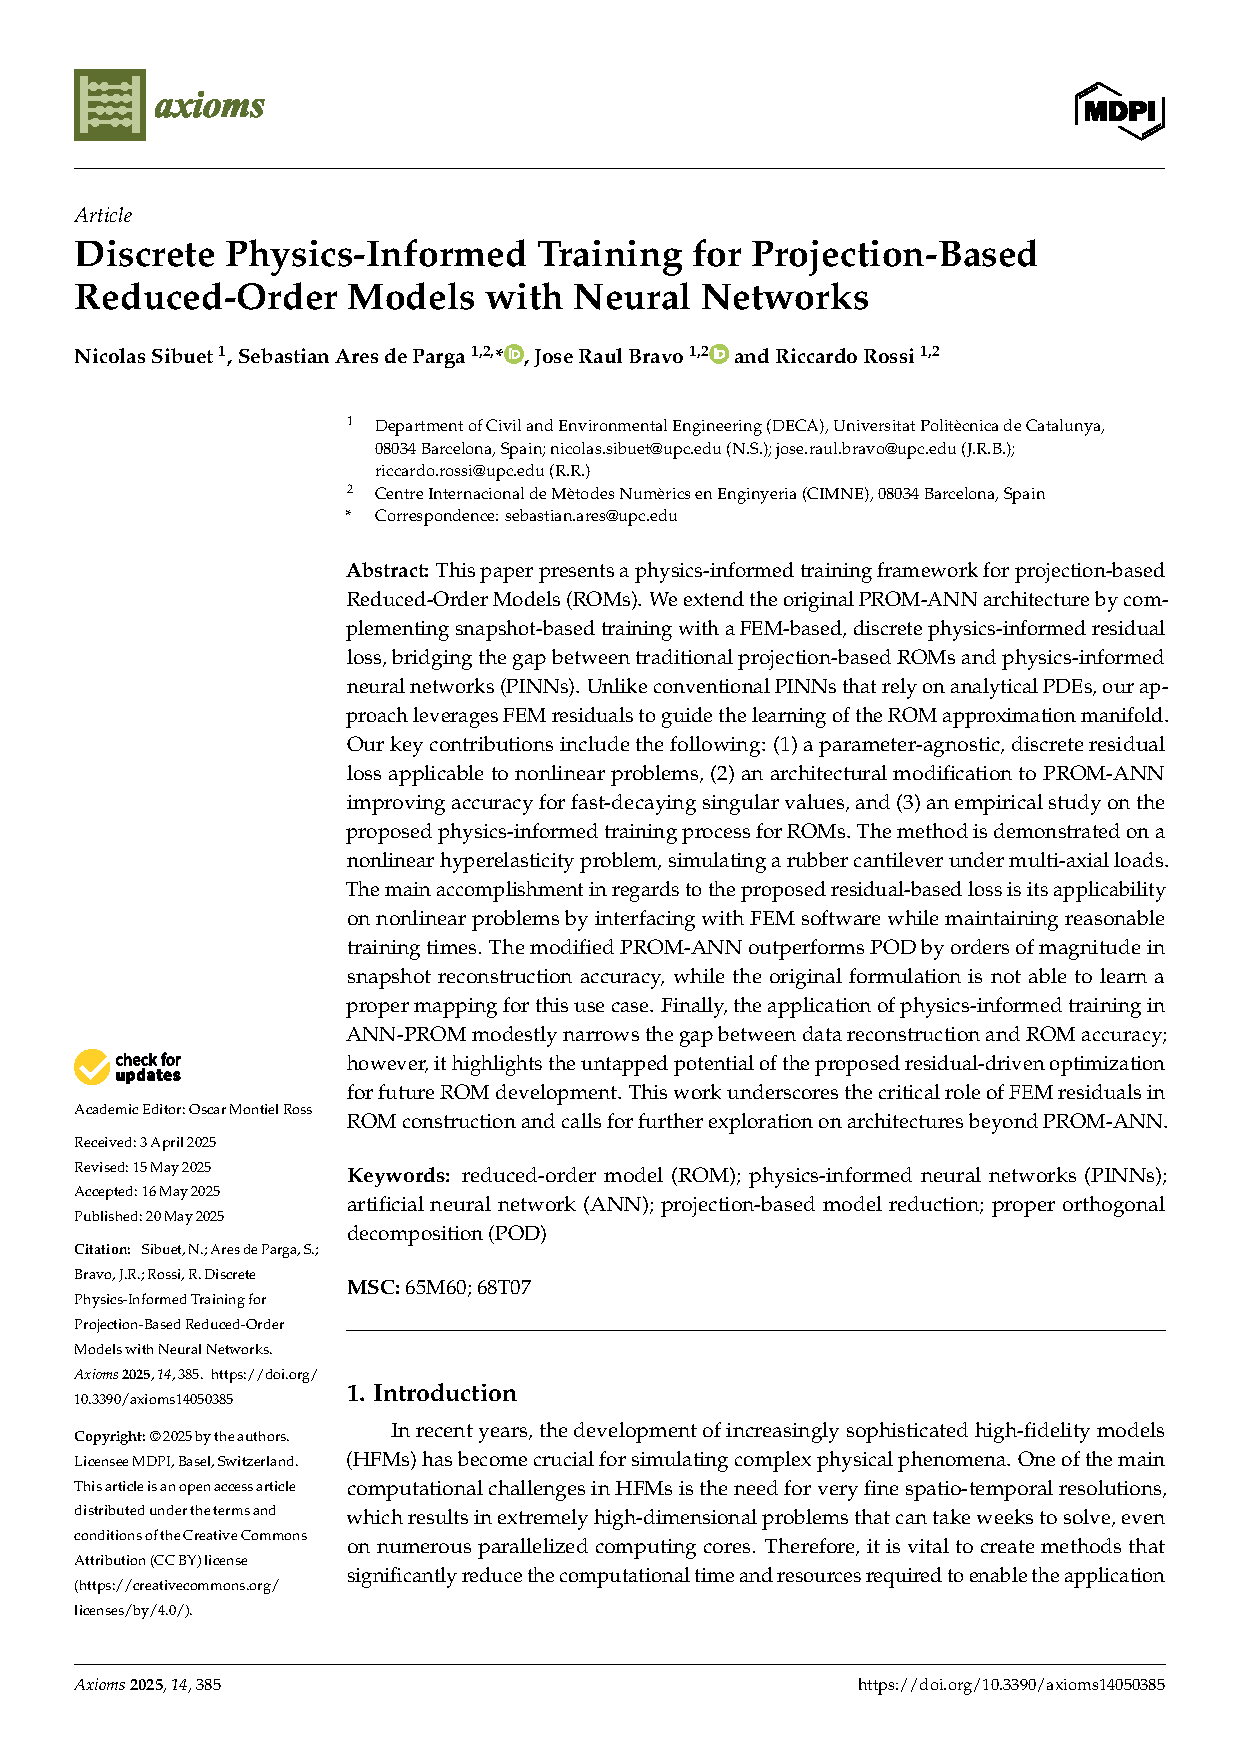
\includepdf[
  pages=-,
  pagecommand={},
  scale=0.92,
  delta=0 0,
  offset=32pt 0pt,
  turn=false
]{Papers/Discrete_Physics-Informed_Training_for_Projection-Based_Reduced-Order_Models_with_Neural_Networks.pdf}


% % CHAPTER 8 - Article 4
\chapter{Nonlinear projection-based model order reduction using machine learning regression to model closure error in the latent space (Article from International Research Stay)}
\label{chap:article4}
This chapter presents the article titled \emph{``Nonlinear projection-based model order reduction using machine learning regression to model closure error in the latent space''}~\cite{de2025nonlinear}, published in \textit{Computer Methods in Applied Mechanics and Engineering} (CMAME). This work was carried out as part of a long-term Fulbright predoctoral research stay as a Visiting Researcher at Stanford University within the research group of Professor Charbel Farhat.

Building on the latent-space closure modeling framework introduced in earlier chapters, this contribution investigates alternative, more interpretable regression strategies that address key limitations of PROM-ANN, such as its reliance on black-box neural networks and large training datasets. Specifically, it proposes Gaussian Process Regression (PROM-GPR) and Radial Basis Function interpolation (PROM-RBF) as kernel-based surrogates for modeling closure errors in the latent space, preserving the flexibility of the nonlinear manifold while enhancing interpretability, data efficiency, and potential certification.

The paper demonstrates:
\begin{itemize}
    \item A unified formulation of PROM-GPR and PROM-RBF within the general nonlinear manifold ROM framework, including analytical expressions for the kernel-based closure maps and their derivatives.
    \item The integration of these regression surrogates into the residual-minimizing Petrov--Galerkin projection and their compatibility with project-then-approximate hyper-reduction techniques.
    \item Validation on industrial-like cases, including a detached-eddy simulation of the Ahmed body wake flow and the two-dimensional inviscid Burgers' equation, illustrating how the approach delivers accuracy comparable to PROM-ANN with significantly reduced training data requirements.
\end{itemize}

This study showcases how kernel-based regression strategies, coupled with robust projection and hyper-reduction frameworks, can effectively mitigate the effects of the Kolmogorov $n$-width barrier in convection-dominated and strongly nonlinear systems. It represents a key contribution of this thesis toward scalable, interpretable, and industry-relevant nonlinear PROMs.

\includepdf[
  pages=-,
  pagecommand={},
  scale=0.92,
  delta=0 0,
  offset=32pt 0pt,
  turn=false
]{Papers/Nonlinear_projection_based_model_order_reduction_with_machine_learning_regression_for_closure_error_modeling_in_the_latent_space.pdf}



% CHAPTER 9 - Conclusion and Future Work
\chapter{Conclusions and Future Work}

This final chapter summarizes the main contributions and methodological advances achieved throughout the thesis and outlines recommended directions for future work and technology transfer.

\section*{Conclusions}

This thesis systematically advances the state of the art in both linear and nonlinear projection-based reduced order modeling by developing, implementing, and rigorously assessing new methodologies across a range of test cases, from canonical model problems to realistic industrial configurations. Key contributions include the formulation of robust hyper-reduction strategies for Petrov–Galerkin PROMs, the design of scalable HPC-enabled workflows for intrusive ROM training, and the development of novel nonlinear manifold approaches, such as PROM-ANN, PROM-GPR, and PROM-RBF, that mitigate the Kolmogorov $n$-width barrier.

A significant practical outcome is the extension of two open-source frameworks, Kratos Multiphysics and AERO-F, to support these advanced ROM techniques, enabling systematic testing from simplified problems like the Burgers equation to complex scenarios including nonlinear structural mechanics, incompressible Navier–Stokes flows, compressible aerodynamic benchmarks, and multiphysics cases such as the thermal dynamics of an electric motor in collaboration with Siemens and the Ahmed body wake flow problem in collaboration with the Farhat Research Group at Stanford University. This validation across diverse physical phenomena illustrates both the generality and robustness of the proposed methodologies.

While this thesis primarily focused on the development and rigorous evaluation of projection-based ROMs, it is important to note that no full digital twin was implemented. The PROMs developed here remain on the testing side and have not yet been connected to live physical assets, a prerequisite for realizing the closed-loop functionality of a true digital twin. Accordingly, the work presented can be seen as laying the foundation for future \textit{Component Twins} and \textit{Asset Twins}: digital representations of individual parts or complete physical assets that can be integrated into broader digital twin ecosystems.

Lastly, the impact of this work extends beyond academic contributions by planting a seed for technology transfer through the \textit{SimTwins} spin-off initiative. This effort aims to leverage the open-source capabilities of projection-based ROMs to deliver scalable digital shadows and digital twins that meet the emerging demands of Industry 4.0 and 5.0, thus positioning projection-based ROM techniques as central enabling technologies in the current and future deep-tech landscape.

\section*{Future Work}

Building on the findings and methodologies established in this thesis, several avenues are recommended for future research and development:
\begin{itemize}
    \item \textbf{Piecewise nonlinear closure modeling:} Extend nonlinear latent-space closure strategies (PROM-ANN, PROM-RBF, PROM-GPR) to piecewise or local subspace frameworks, leveraging Local POD or clustering strategies. This will further enhance efficiency and accuracy in complex, strongly nonlinear, or convection-dominated industrial problems.
    
    \item \textbf{Physics-embedded machine learning:} Further refine and expand methods that embed governing physics into machine learning-based ROMs, including residual-consistent training (such as the discrete physics-informed strategy demonstrated here) and projection-based hybrid formulations. Prioritize such approaches in settings where governing equations are available, thereby strengthening the reliability and robustness of forward simulations in industrial contexts.
    
    \item \textbf{Broader industrial application:} Expand these ROM techniques into increasingly challenging industrial configurations, particularly hypersonic flows and multiphysics models with extensive parametric spaces. Such applications will fully leverage and demonstrate the scalability and computational efficiency achievable by projection-based ROMs.
    
    \item \textbf{Closing the digital twin loop:} Focus efforts on integrating developed PROMs with real-time sensor data and physical assets, transitioning from robustly tested surrogates into operational \textit{Component Twins} and \textit{Asset Twins}. This integration is essential for continuous monitoring, adaptation, and real-time decision support capabilities in practical engineering systems.
    
    \item \textbf{Support for open-source frameworks and technology transfer:} Continue enhancing, maintaining, and contributing to open-source frameworks such as Kratos Multiphysics and AERO-F, ensuring advanced ROM techniques remain widely accessible. Simultaneously, further development through the \textit{SimTwins} initiative will be crucial for translating research advances into practical and industry-ready ROM-based solutions.
\end{itemize}

Together, these future directions aim to consolidate the impact of this thesis and further position projection-based reduced order modeling as a robust, scalable, and physically consistent tool for real-time digital twins and next-generation engineering applications.


% APPENDIX
\appendix
\chapter{Appendix}

\section{Crank--Nicolson time discretization (inviscid with SUPG)}
\label{appendix:cranknicolson}

The Crank--Nicolson (CN) scheme is a second-order, A-stable, implicit method obtained by applying the trapezoidal rule in time.  When it is applied to the spatially discretised, inviscid Burgers’ equation, including any Streamline-Upwind/Petrov–Galerkin (SUPG) stabilisation, the fully discrete equation for each time step $n\to n+1$ reads
%
\begin{equation}
\mathbf M \,\frac{\mathbf u^{n+1}-\mathbf u^{n}}{\Delta t}
\;+\;
\frac12\Bigl[
   \mathbf C\!\bigl(\mathbf u^{n}\bigr)\,\mathbf u^{n}
  +\mathbf C\!\bigl(\mathbf u^{n+1}\bigr)\,\mathbf u^{n+1}
\Bigr]
\;+\;
\frac12\Bigl[
   \mathbf S\!\bigl(\mathbf u^{n}\bigr)
  +\mathbf S\!\bigl(\mathbf u^{n+1}\bigr)
\Bigr]
\;=\;
\frac12\bigl(\mathbf F^{n}+\mathbf F^{n+1}\bigr),
\label{eq:cn_supg}
\end{equation}
%
where

\begin{itemize}
  \item $\mathbf M$ is the (constant) mass matrix,
  \item $\mathbf C(\mathbf u)$ is the nonlinear convection \emph{operator} and
        $\mathbf C(\mathbf u)\mathbf u$ its associated convective \emph{term},
  \item $\mathbf S(\mathbf u)$ is the SUPG stabilisation term,
  \item $\mathbf F^{n}$ is the external load vector at $t^{n}$,
  \item $\Delta t$ is the time step,
  \item $\mathbf u^{n}$, $\mathbf u^{n+1}$ are the nodal state vectors at
        $t^{n}$ and $t^{n+1}$.
\end{itemize}

\paragraph{Remarks.}
\begin{enumerate}
  \item The arithmetic average 
        $\tfrac12\!\left[\mathbf S(\mathbf u^{n})+\mathbf S(\mathbf u^{n+1})\right]$
        is the trapezoidal (Crank–Nicolson) quadrature for the stabilisation term and
        yields global second-order accuracy.  A common alternative that also achieves
        second order is to evaluate $\mathbf S$ at a midpoint in time,
        $\mathbf S(\mathbf u^{n+\frac12})$.  However,
        $\tfrac12\!\left[\mathbf S(\mathbf u^{n})+\mathbf S(\mathbf u^{n+1})\right]
        = \mathbf S\!\left(\tfrac{\mathbf u^{n}+\mathbf u^{n+1}}{2}\right)$
        holds only if $\mathbf S$ is linear (affine) in $\mathbf u$.  For nonlinear
        $\mathbf S$, the two forms are not algebraically identical (though both are
        second-order accurate), and using the arithmetic state average
        $\mathbf u^{n+\frac12}=\tfrac12(\mathbf u^{n}+\mathbf u^{n+1})$ does not in
        general coincide with the true mid-time state.
  \item CN is A-stable but not L-stable; in convection-dominated problems it may
        exhibit weak, non-damping oscillations compared with backward Euler.
        Consequently smaller $\Delta t$ or selective filtering may be required if
        very sharp shocks are present.
  \item Equation~\eqref{eq:cn_supg} is nonlinear because the convective and
        stabilisation terms depend on the unknown $\mathbf u^{n+1}$.  Each time step
        therefore requires the solution of a nonlinear system, typically by a Picard
        (frozen-convection) or Newton iteration.
\end{enumerate}


\section{Finite volume discretization of the inviscid Burgers' equation with source term}
\label{appendix:fvm_burgers}
We consider the one-dimensional inviscid Burgers' equation augmented by a spatially varying source term:
\begin{equation}
\frac{\partial u(x,t)}{\partial t} + u(x,t)\,\frac{\partial u(x,t)}{\partial x} = s(x,t),
\quad \forall x \in [0, L],\quad \forall t \in [0, T],
\label{eq:burgers_strong}
\end{equation}
where \( u(x,t) \) is the unknown solution (e.g., a velocity field), and \( s(x,t) \) is a prescribed source term that may depend on space and time.%
\footnote{In the finite element formulation, the source term is denoted \( f(x,t) \). Here \( s(x,t) \) is used instead to avoid conflict with the flux function notation \( f = \frac{1}{2} u^2 \) typically used in finite volume schemes.}
This equation represents a nonlinear, first-order, time-dependent conservation law with a forcing term.

\subsection{Spatial discretization and control volumes}

To apply the finite volume method (FV), the spatial domain \( [0, L] \) is divided into \( N \) non-overlapping control volumes (cells), each of uniform width \( \Delta x \). The \( i \)-th cell is bounded by the interfaces \( x_{i-1/2} \) and \( x_{i+1/2} \), with center at \( x_i \). The solution is represented in terms of its \textit{cell average}:
\begin{equation}
\bar{u}_i(t) := \frac{1}{\Delta x} \int_{x_{i-1/2}}^{x_{i+1/2}} u(x,t)\,\mathrm{d}x.
\label{eq:cell_average}
\end{equation}
The discrete vector of cell averages is defined as
\begin{equation}
\bar{\mathbf{u}}(t) := \begin{bmatrix} \bar{u}_1(t) & \bar{u}_2(t) & \cdots & \bar{u}_N(t) \end{bmatrix}^\top \in \mathbb{R}^N,
\end{equation}
in analogy with the nodal solution vector \( \mathbf{u}(t) \) used in the finite element formulation.

\subsection{Integral form of the conservation law}

To derive the finite volume formulation, the governing equation \eqref{eq:burgers_strong} is integrated over the spatial control volume \( [x_{i-1/2}, x_{i+1/2}] \):
\begin{equation}
\int_{x_{i-1/2}}^{x_{i+1/2}} 
\left( \frac{\partial u}{\partial t} + u\,\frac{\partial u}{\partial x} \right)\,\mathrm{d}x 
= \int_{x_{i-1/2}}^{x_{i+1/2}} s(x,t)\,\mathrm{d}x.
\label{eq:fv_integral}
\end{equation}

Each term in \eqref{eq:fv_integral} is analyzed separately below.

\subsubsection*{Time derivative term}

Applying the definition of the cell average \eqref{eq:cell_average} yields:
\begin{equation}
\int_{x_{i-1/2}}^{x_{i+1/2}} \frac{\partial u}{\partial t}\,\mathrm{d}x 
= \Delta x \cdot \frac{\mathrm{d} \bar{u}_i(t)}{\mathrm{d}t}.
\end{equation}

\subsubsection*{Convective term and conservative form}

The convective term is nonlinear, but can be expressed in conservative form via the identity:
\begin{equation}
u \, \frac{\partial u}{\partial x} = \frac{\partial}{\partial x} \left( \frac{1}{2} u^2 \right),
\end{equation}
which follows directly from the chain rule. Substituting into the integral yields:
\begin{equation}
\int_{x_{i-1/2}}^{x_{i+1/2}} u\,\frac{\partial u}{\partial x}\,\mathrm{d}x 
= \int_{x_{i-1/2}}^{x_{i+1/2}} \frac{\partial}{\partial x} \left( \frac{1}{2} u^2 \right)\,\mathrm{d}x.
\end{equation}
Applying the \textit{Fundamental Theorem of Calculus} gives:
\begin{equation}
\int_{x_{i-1/2}}^{x_{i+1/2}} \frac{\partial}{\partial x} \left( \frac{1}{2} u^2 \right)\,\mathrm{d}x 
= \left. \frac{1}{2} u^2 \right|_{x_{i-1/2}}^{x_{i+1/2}} 
= f_{i+1/2} - f_{i-1/2},
\label{eq:fv_flux_difference}
\end{equation}
where the \textit{numerical fluxes} \( f_{i\pm1/2} \) across each interface are defined by:
\begin{equation}
f_{i+1/2} := \left. \frac{1}{2} u^2 \right|_{x_{i+1/2}}, \quad
f_{i-1/2} := \left. \frac{1}{2} u^2 \right|_{x_{i-1/2}}.
\end{equation}
These fluxes will later be approximated using a suitable Riemann solver (e.g., Godunov flux).%
\footnote{In contrast to the finite element method, where stabilization (e.g., SUPG) is introduced to handle convective dominance, the finite volume approach employs numerical fluxes (such as Godunov flux) that inherently stabilize the solution by capturing shocks and discontinuities.}

\subsubsection*{Source term}

The integral of the source term is approximated using the midpoint rule:
\begin{equation}
\int_{x_{i-1/2}}^{x_{i+1/2}} s(x,t)\,\mathrm{d}x 
\;\approx\; 
\Delta x \cdot \bar{s}_i(t),
\end{equation}
where \( \bar{s}_i(t) := s(x_i,t) \) denotes the source term evaluated at the cell center.

\subsection{Semi-discrete finite volume formulation}

Collecting the contributions of the time derivative, convective, and source terms, and dividing by \( \Delta x \), the semi-discrete finite volume formulation becomes:
\begin{equation}
\frac{\mathrm{d} \bar{u}_i(t)}{\mathrm{d}t}
= - \frac{1}{\Delta x} \left( f_{i+1/2} - f_{i-1/2} \right) + \bar{s}_i(t),
\label{eq:fv_semidiscrete}
\end{equation}
where:
\begin{itemize}
    \item \( \bar{u}_i(t) \) is the cell average of the solution,
    \item \( f_{i\pm1/2} \) are the numerical fluxes at interfaces,
    \item \( \bar{s}_i(t) \) is the cell-centered source term.
\end{itemize}

This equation represents the finite volume counterpart to the Galerkin semi-discrete FEM formulation and provides the basis for subsequent time discretization and nonlinear solver development.


\subsection{Time discretization}

To advance the semi-discrete system \eqref{eq:fv_semidiscrete} in time, a first-order accurate \textit{Backward Euler} method is employed.\footnote{The Backward Euler scheme is adopted for consistency with the time discretization used in the finite element formulation and due to its robustness in convection-dominated regimes.} Let \( \Delta t \) denote the time step, and let \( \bar{u}_i^n \) and \( \bar{u}_i^{n+1} \) represent the cell-averaged solutions at time levels \( t^n \) and \( t^{n+1} = t^n + \Delta t \), respectively. The time derivative is approximated as:
\begin{equation}
\frac{\mathrm{d} \bar{u}_i(t)}{\mathrm{d}t} 
\;\approx\;
\frac{\bar{u}_i^{n+1} - \bar{u}_i^n}{\Delta t}.
\end{equation}

Substituting this approximation into \eqref{eq:fv_semidiscrete} yields the fully discrete form:
\begin{equation}
\frac{\bar{u}_i^{n+1} - \bar{u}_i^n}{\Delta t}
= - \frac{1}{\Delta x} \left( f_{i+1/2}^{n+1} - f_{i-1/2}^{n+1} \right) + \bar{s}_i^{n+1},
\label{eq:fv_fully_discrete}
\end{equation}
or equivalently,
\begin{equation}
\bar{u}_i^{n+1} = \bar{u}_i^n - \frac{\Delta t}{\Delta x} \left( f_{i+1/2}^{n+1} - f_{i-1/2}^{n+1} \right) + \Delta t \cdot \bar{s}_i^{n+1}.
\end{equation}

This formulation is \textit{implicit}, as the numerical fluxes \( f_{i\pm1/2}^{n+1} \) depend on the unknown solution \( \bar{u}^{n+1} \). Therefore, a nonlinear system must be solved at each time step. To define this system explicitly, the \textit{residual function} is introduced:
\begin{equation}
R_i\left( \bar{u}^{n+1} \right) := 
\bar{u}_i^{n+1} - \bar{u}_i^n 
+ \frac{\Delta t}{\Delta x} \left( f_{i+1/2}^{n+1} - f_{i-1/2}^{n+1} \right) 
- \Delta t \cdot \bar{s}_i^{n+1},
\label{eq:fv_residual}
\end{equation}
such that solving the finite volume system corresponds to finding \( \bar{\mathbf{u}}^{n+1} \in \mathbb{R}^N \) that satisfies:
\begin{equation}
\mathbf{R}(\bar{\mathbf{u}}^{n+1}) = \mathbf{0},
\label{eq:residual_fv}
\end{equation}

\subsection{Numerical flux approximation via the Godunov method}

To fully specify the residual \eqref{eq:fv_residual}, a numerical flux approximation must be provided for evaluating the convective terms \( f_{i+1/2}^{n+1} \) and \( f_{i-1/2}^{n+1} \). In the finite volume context, these fluxes depend on the values of the solution to the left and right of each interface. However, since only the cell-average \( \bar{u}_i \) is known in each control volume, interface values must be reconstructed from this cell-average data.

\paragraph{Constant Reconstruction.} A \textit{constant reconstruction} is adopted, assuming that the solution within each control volume is constant and equal to the cell average:
\[
u(x,t) \approx \bar{u}_i(t), \quad \forall x \in [x_{i-1/2}, x_{i+1/2}].
\]
This approximation yields the left and right states at each interface \( x_{i+1/2} \) as:
\[
u_L = \bar{u}_i, \qquad u_R = \bar{u}_{i+1}.
\]

This approach eliminates the need for slope reconstruction and limiting strategies, making it particularly robust in the presence of shocks or discontinuities. It also aligns naturally with the derivation assumptions underlying the \textit{Godunov flux} described below.

\paragraph{Riemann Problem.} The Godunov method computes numerical fluxes at interfaces by solving the following local Riemann problem:
\begin{equation}
\frac{\partial u}{\partial t} + \frac{\partial}{\partial x}\left( \frac{1}{2} u^2 \right) = 0,
\qquad
u(x,0) = 
\begin{cases}
u_L, & x < 0, \\
u_R, & x > 0,
\end{cases}
\label{eq:burgers_riemann}
\end{equation}
where \( u_L = \bar{u}_i \) and \( u_R = \bar{u}_{i+1} \) represent the reconstructed solution values to the left and right of the interface \( x_{i+1/2} \).

The solution \( u^\star \) to the Riemann problem at the interface (at \( x = 0 \), \( t > 0 \)) defines the Godunov numerical flux:
\begin{equation}
f^{\text{Godunov}}(u_L, u_R) := \frac{1}{2}(u^\star)^2.
\end{equation}

For the scalar Burgers' equation, the Riemann problem admits an exact solution that depends on the relationship between \( u_L \) and \( u_R \):

\begin{itemize}
    \item \textbf{Shock:} If \( u_L > u_R \), the solution forms a shock wave propagating with speed given by the \emph{Rankine--Hugoniot condition}:
    \[
    s = \frac{f(u_R) - f(u_L)}{u_R - u_L} 
    = \frac{\frac{1}{2}u_R^2 - \frac{1}{2}u_L^2}{u_R - u_L}
    = \frac{1}{2}(u_L + u_R).
    \]
    The state at the interface is:
    \[
    u^\star = 
    \begin{cases}
    u_L, & \text{if } s > 0, \\
    u_R, & \text{if } s < 0.
    \end{cases}
    \]

    \item \textbf{Rarefaction:} If \( u_L < u_R \), a centered rarefaction wave forms, with characteristics spreading between \( u_L \) and \( u_R \). The interface value is determined by the characteristic direction:
    \[
    u^\star = 
    \begin{cases}
    u_L, & \text{if } 0 < u_L, \\
    u_R, & \text{if } 0 > u_R, \\
    0,   & \text{if } u_L < 0 < u_R.
    \end{cases}
    \]
\end{itemize}

No flux splitting or directional notation (such as \( u^- \), \( u^+ \)) is required for this scalar problem since wave propagation behavior is completely determined by the Riemann solution. This is unlike systems of equations, where multiple characteristic fields and flux components may require directional decomposition.

The explicit form of the Godunov flux thus becomes:
\begin{equation}
f^{\text{Godunov}}(u_L, u_R) =
\begin{cases}
\frac{1}{2} u_L^2, & u_L > u_R \text{ and } \frac{1}{2}(u_L + u_R) > 0, \\
\frac{1}{2} u_R^2, & u_L > u_R \text{ and } \frac{1}{2}(u_L + u_R) < 0, \\
\frac{1}{2} u_L^2, & u_L \le u_R \text{ and } 0 \le u_L, \\
\frac{1}{2} u_R^2, & u_L \le u_R \text{ and } 0 \ge u_R, \\
0,                & u_L \le u_R \text{ and } u_L < 0 < u_R.
\end{cases}
\label{eq:godunov_flux}
\end{equation}

This flux formulation accurately captures shock and rarefaction behavior without requiring artificial dissipation or flux limiters. It is directly utilized to evaluate the interface terms \( f_{i+1/2}^{n+1} \) and \( f_{i-1/2}^{n+1} \) in the residual \eqref{eq:fv_residual}, defining the nonlinear system solved at each time step.

\subsection{Boundary conditions}

To evaluate the numerical fluxes at domain boundaries, the finite volume method requires solution values at the "ghost cells" located beyond the physical domain. Let \( \bar{u}_0 \) and \( \bar{u}_{N+1} \) denote these ghost cell values adjacent to the first and last control volumes, respectively.

A Dirichlet inflow condition at the left boundary is enforced as:
\begin{equation}
u(0,t) = u_{\text{left}}(t) = \mu_1,\end{equation}
by setting the left ghost cell as:
\begin{equation}\bar{u}_0^{n+1} := \mu_1(t^{n+1}).\end{equation}

At the right boundary, where explicit boundary data are not specified, a \textit{zero-gradient} (Neumann-type) outflow condition is adopted:
\begin{equation}\bar{u}_{N+1}^{n+1} := \bar{u}_N^{n+1}.\end{equation}

These boundary values are utilized to compute numerical fluxes at the domain interfaces \( f_{1/2}^{n+1} \) and \( f_{N+1/2}^{n+1} \), ensuring that the residuals \( R_1 \) and \( R_N \) are properly defined\footnote{In finite volume methods, ghost cell values are required to compute boundary fluxes. In finite element methods, Neumann conditions arise only when diffusion is present; in pure advection, only Dirichlet conditions need to be enforced.}.

\paragraph{Remark.} Alternative treatments, such as extrapolation or characteristic-based conditions, can be employed depending on problem specifics. The approach presented here prioritizes simplicity and consistency with standard finite volume implementations for scalar conservation laws.

\subsection{Nonlinear system and Newton--Raphson method}

Following the time discretization and flux approximations outlined in \eqref{eq:fv_fully_discrete}--\eqref{eq:fv_residual}, each time step \(n\) involves solving:
\begin{equation}
\mathbf{R}\bigl(\bar{\mathbf{u}}^{n+1}\bigr) = \mathbf{0},
\quad \text{where} \quad
R_i\bigl(\bar{u}^{n+1}\bigr)
=
\bar{u}_i^{n+1}
-
\bar{u}_i^n
+
\frac{\Delta t}{\Delta x}\left(
 f_{i+1/2}^{n+1} - f_{i-1/2}^{n+1}
\right)
-
\Delta t\,\bar{s}_i^{n+1},
\label{eq:fv_Ri_recall}
\end{equation}
and \(f_{i\pm1/2}^{n+1}=f^{\text{Godunov}}(\bar{u}_i^{n+1},\bar{u}_{i\pm1}^{n+1})\) are the nonlinear numerical fluxes evaluated at the unknown solution \(\bar{\mathbf{u}}^{n+1}\). Thus, \eqref{eq:fv_Ri_recall} forms a nonlinear algebraic system analogous to the nonlinear residual system in the finite element formulation (cf. Eq.~\eqref{eq:R_supg_inviscid}).

\paragraph{Newton--Raphson linearization.}
To efficiently solve \eqref{eq:fv_Ri_recall}, the Newton--Raphson method is applied. Let \(\bar{\mathbf{u}}^{(k)}\) represent the current iterate for solution \(\bar{\mathbf{u}}^{n+1}\). Expanding the residual around \(\bar{\mathbf{u}}^{(k)}\) yields:
\begin{equation}
\mathbf{R}\bigl(\bar{\mathbf{u}}^{(k+1)}\bigr)
\approx
\mathbf{R}\bigl(\bar{\mathbf{u}}^{(k)}\bigr)
+
\mathbf{J}\bigl(\bar{\mathbf{u}}^{(k)}\bigr)\left(\bar{\mathbf{u}}^{(k+1)} - \bar{\mathbf{u}}^{(k)}\right),
\end{equation}
where \(\mathbf{J}(\bar{\mathbf{u}}^{(k)})=\frac{\partial\mathbf{R}}{\partial\bar{\mathbf{u}}}\bigl(\bar{\mathbf{u}}^{(k)}\bigr)\) is the Jacobian matrix. Setting \(\mathbf{R}\bigl(\bar{\mathbf{u}}^{(k+1)}\bigr)=\mathbf{0}\) results in the Newton iteration:
\begin{equation}
\mathbf{J}\bigl(\bar{\mathbf{u}}^{(k)}\bigr)\,\delta\bar{\mathbf{u}}^{(k)}
=-\mathbf{R}\bigl(\bar{\mathbf{u}}^{(k)}\bigr),\quad\text{where}\quad
\delta\bar{\mathbf{u}}^{(k)}=\bar{\mathbf{u}}^{(k+1)}-\bar{\mathbf{u}}^{(k)}.
\label{eq:fv_newton_global}
\end{equation}

\paragraph{Jacobian assembly.}
The residual \(R_i\) depends only on local cell averages \(\bar{u}_{i-1}, \bar{u}_i, \bar{u}_{i+1}\), resulting in a tridiagonal structure similar to that encountered in finite element discretizations. The Jacobian entries are explicitly derived from the Godunov flux definition \eqref{eq:godunov_flux}:
\begin{align*}
\frac{\partial R_i}{\partial \bar{u}_{i-1}} &=
    -\frac{\Delta t}{\Delta x}
    \frac{\partial f^{\text{Godunov}}}{\partial u_L}\bigg|_{i-1/2},
\\[0.5em]
\frac{\partial R_i}{\partial \bar{u}_i} &=
    1 + \frac{\Delta t}{\Delta x} \left(
    \frac{\partial f^{\text{Godunov}}}{\partial u_L}\bigg|_{i+1/2}
    - \frac{\partial f^{\text{Godunov}}}{\partial u_R}\bigg|_{i-1/2}
    \right),
\\[0.5em]
\frac{\partial R_i}{\partial \bar{u}_{i+1}} &=
    \frac{\Delta t}{\Delta x}
    \frac{\partial f^{\text{Godunov}}}{\partial u_R}\bigg|_{i+1/2}.
\end{align*}


\paragraph{Implementation remark.}
Analytical differentiation of the Godunov flux ensures an accurate Jacobian matrix, which enhances Newton convergence compared to a numerical Jacobian obtained via finite differences, analogous to common practice in finite element implementations.

\paragraph{Linear system solution and update.}
The linear system \eqref{eq:fv_newton_global} is solved using standard sparse solvers. The iterate is updated as:
\begin{equation}
\bar{\mathbf{u}}^{(k+1)}
=\bar{\mathbf{u}}^{(k)}+\delta\bar{\mathbf{u}}^{(k)},
\end{equation}
and iteration proceeds until a suitable convergence criterion, such as \(\|\mathbf{R}(\bar{\mathbf{u}}^{(k)})\|\leq\text{tolerance}\), is satisfied.

\paragraph{Discussion and convergence.}
Newton--Raphson typically exhibits quadratic convergence near the solution, provided a good initial guess (usually \(\bar{\mathbf{u}}^{(0)}=\bar{\mathbf{u}}^{n}\)). Although each iteration is computationally more demanding than a simpler fixed-point (Picard) iteration, the overall rapid convergence makes Newton--Raphson a robust and efficient choice for implicit finite volume discretizations of nonlinear conservation laws. This parallels the FEM practice discussed in Section~\ref{sec:fem_discretization}.

\section{Finite difference discretization of the inviscid Burgers' equation with source term}
\label{appendix:fd_burgers}

This section presents a finite difference (FD) discretization for the inviscid one-dimensional Burgers' equation with a source term, employing second-order central differences, implicit (Backward Euler) time integration, artificial viscosity stabilization, and Newton--Raphson nonlinear solving. The formulation closely mirrors the previously presented finite element and finite volume methods.

\subsection{Strong Form of the Governing Equation}

We consider the following scalar conservation law:
\begin{equation}
\frac{\partial u(x,t)}{\partial t} + u(x,t)\frac{\partial u(x,t)}{\partial x} = s(x,t), \quad x \in [0, L],\quad t \in [0, T],
\label{eq:fd_strongform}
\end{equation}
with the boundary and initial conditions:
\begin{equation}
u(0,t)=\mu_1,\quad u(x,0)=u_{\text{initial}}(x), \quad \forall x \in [0,L].\end{equation}
The source term is explicitly defined as:
\begin{equation}
s(x,t) = 0.02\,e^{\mu_2\,x}.
\end{equation}

\subsection{Spatial discretization}

The spatial domain \([0,L]\) is partitioned into \(N\) uniformly distributed nodes:
\begin{equation}
x_i = i\Delta x, \quad \Delta x = \frac{L}{N-1}, \quad i = 0,1,\dots,N-1,
\end{equation}
and we denote \(u_i(t)\approx u(x_i,t)\). \\
The nodal values are gathered into the vector \(\mathbf{u}(t) = [u_0(t),u_1(t),\dots,u_{N-1}(t)]^\top\).

\paragraph{Convection and Stabilization.} The spatial derivative of the convective flux \(\frac{1}{2}u^2\) is approximated using second-order central differences with an artificial viscosity term for stabilization:
\begin{equation}
\frac{\partial}{\partial x}\left(\frac{1}{2}u^2\right)\bigg|_{x_i}\approx \frac{\frac{1}{2}u_{i+1}^2-\frac{1}{2}u_{i-1}^2}{2\Delta x} - \nu_{\text{artificial}}\frac{u_{i+1}-2u_i+u_{i-1}}{\Delta x^2},
\label{eq:fd_conv}
\end{equation}
where the artificial viscosity is chosen adaptively as:
\begin{equation}
\nu_{\text{artificial}} = 0.25\,\Delta x\,\max_{i}|u_i|.
\end{equation}
This term provides numerical stability by damping spurious oscillations common in convection-dominated problems.

\subsection{Implicit time integration}

To integrate in time, the implicit Backward Euler scheme is utilized:
\begin{equation}
\frac{u_i^{n+1}-u_i^n}{\Delta t}+\frac{\frac{1}{2}(u_{i+1}^{n+1})^2-\frac{1}{2}(u_{i-1}^{n+1})^2}{2\Delta x}-\nu_{\text{artificial}}\frac{u_{i+1}^{n+1}-2u_i^{n+1}+u_{i-1}^{n+1}}{\Delta x^2}=s_i^{n+1},
\label{eq:fd_fully_discrete}
\end{equation}
where \(u_i^n\approx u_i(t^n)\) and \(s_i^{n+1}=s(x_i,t^{n+1})\). This formulation leads to a nonlinear algebraic system at each time step.

\subsection{Nonlinear residual and Newton--Raphson method}

Defining the residual at node \(i\):
\begin{equation}
R_i(\mathbf{u}^{n+1}) = \frac{u_i^{n+1}-u_i^n}{\Delta t}+\frac{\frac{1}{2}(u_{i+1}^{n+1})^2-\frac{1}{2}(u_{i-1}^{n+1})^2}{2\Delta x}-\nu_{\text{artificial}}\frac{u_{i+1}^{n+1}-2u_i^{n+1}+u_{i-1}^{n+1}}{\Delta x^2}-s_i^{n+1},
\label{eq:residual_fd_component}
\end{equation}

this component-wise expression defines the global nonlinear residual vector:
\begin{equation}
\mathbf{R}(\mathbf{u}^{n+1}) = \mathbf{0}.
\label{eq:residual_fd_vector}
\end{equation}

The Newton--Raphson iteration is then formulated as:
\begin{equation}
\mathbf{J}(\mathbf{u}^{(k)})\delta \mathbf{u}^{(k)} = -\mathbf{R}(\mathbf{u}^{(k)}),\quad \mathbf{u}^{(k+1)}=\mathbf{u}^{(k)}+\delta \mathbf{u}^{(k)},
\label{eq:fd_newton_iteration}
\end{equation}
where \(\mathbf{J}\) is the analytical Jacobian with entries:
\begin{align}
\frac{\partial R_i}{\partial u_{i-1}}&=-\frac{u_{i-1}}{2\Delta x}-\frac{\nu_{\text{artificial}}}{\Delta x^2},\\[5pt]
\frac{\partial R_i}{\partial u_{i}}&=\frac{1}{\Delta t}+\frac{2\nu_{\text{artificial}}}{\Delta x^2},\\[5pt]
\frac{\partial R_i}{\partial u_{i+1}}&=\frac{u_{i+1}}{2\Delta x}-\frac{\nu_{\text{artificial}}}{\Delta x^2}.
\end{align}

Alternatively, a finite-difference approximation of the Jacobian can be employed for validation and debugging.


\subsection{Boundary conditions}

At the left boundary, a Dirichlet inflow condition is enforced:
\begin{equation}
u_0^{n+1}=\mu_1.\end{equation}
At the right boundary, a zero-gradient (Neumann-type) outflow condition is applied:
\begin{equation}
u_{N-1}^{n+1}=u_{N-2}^{n+1}.\end{equation}
These conditions match the implementation details in the finite element and finite volume formulations presented previously.

\paragraph{Remark.} While the Backward Euler scheme introduces additional numerical dissipation, its use here prioritizes robustness and direct consistency with the FEM and FV schemes employed previously. Higher-order schemes could be adopted to reduce numerical diffusion if accuracy requirements demand it.

%======================================================================
\section{Derivation of the Gauss--Newton reduced system on a general manifold}
\label{app:gauss_newton_manifold}
%======================================================================

This appendix collects, in a self-contained form, the detailed steps leading  
from the minimum–residual statement on a general approximation manifold to the
Gauss–Newton linear system that underpins the nonlinear PROM used in
Chapter~\ref{chap:nonlinear_prom}.  All quantities initially retain their
explicit dependence on time~\(t\), parameters~\(\boldsymbol{\mu}\), and the
reduced state~\(\mathbf{q}\); these dependences are suppressed after the
stationarity condition is derived, as indicated in the main text.

%----------------------------------------------------------------------
\subsection{Minimum–residual formulation}
%----------------------------------------------------------------------
Given the decoder \(D_u : \mathbb{R}^{n}\to\mathbb{R}^{N}\), the
reduced coordinates \(\mathbf{q}(t,\boldsymbol{\mu})\in\mathbb{R}^{n}\) are
defined by the weighted least–squares problem
%
\begin{equation}
\min_{\mathbf q\in\mathbb{R}^{n}}
\;\;
\frac12\,
\bigl\|
  \mathbf R\bigl(D_u(\mathbf q);\,t,\boldsymbol\mu\bigr)
\bigr\|_{\mathbf G}^{2},
\qquad
\|\mathbf v\|_{\mathbf G}^{2}:=\mathbf v^{T}\mathbf G\,\mathbf v,\;
\mathbf G\succ0.
\label{eq:A_minres}
\end{equation}

%----------------------------------------------------------------------
\subsection{Stationarity condition}
%----------------------------------------------------------------------
Let
\[
\mathbf J
\bigl(D_u(\mathbf q);\,t,\boldsymbol\mu\bigr)
:=
\frac{\partial\mathbf R}{\partial\mathbf u}
\quad\text{and}\quad
\frac{\partial D_u(\mathbf q)}{\partial\mathbf q}
\in\mathbb{R}^{N\times n}.
\]
Applying the chain rule,
\(
\tfrac{\partial\mathbf R}{\partial\mathbf q}
      =\mathbf J\,\tfrac{\partial D_u}{\partial\mathbf q}.
\)
The gradient of~\eqref{eq:A_minres} with respect to \(\mathbf q\) is therefore
\(
(\mathbf J\,\tfrac{\partial D_u}{\partial\mathbf q})^{T}
\mathbf G\,
\mathbf R,
\)
and the first-order optimality condition is
%
\begin{equation}
\left(
 \frac{\partial D_u}{\partial\mathbf q}
\right)^{T}
\mathbf J^{T}
\mathbf G\,
\mathbf R = \mathbf 0.
\label{eq:A_stationarity}
\end{equation}

%----------------------------------------------------------------------
\subsection{Reduced residual and its Jacobian}
%----------------------------------------------------------------------
Define the \emph{encoded residual}
\begin{equation}
E_r(\mathbf R):=
\left(
 \frac{\partial D_u}{\partial\mathbf q}
\right)^{T}
\mathbf J^{T}
\mathbf G\,\mathbf R
\quad\Longrightarrow\quad
\mathbf r(\mathbf q):=
E_r\bigl(\mathbf R(D_u(\mathbf q))\bigr)=\mathbf 0.
\label{eq:A_encodedResidual}
\end{equation}

Differentiating~\eqref{eq:A_encodedResidual} with respect to \(\mathbf q\)
gives the exact Jacobian
%
\begin{align}
\frac{\partial\mathbf r}{\partial\mathbf q}
&=
\left(
 \frac{\partial D_u}{\partial\mathbf q}
\right)^{T}
\mathbf J^{T}
\mathbf G\,
\mathbf J
\left(
 \frac{\partial D_u}{\partial\mathbf q}
\right)
\notag\\[4pt]
&\quad
+
\underbrace{
\left(
 \frac{\partial D_u}{\partial\mathbf q}
\right)^{T}
\Bigl(
      \partial_{\mathbf u}(\mathbf J^{T}\mathbf G\mathbf R)
 \Bigr)
 \frac{\partial D_u}{\partial\mathbf q}
}_{\text{variation of }\mathbf J}
\;+\;
\underbrace{
\frac{\partial}{\partial\mathbf q}
\Bigl(
 \tfrac{\partial D_u}{\partial\mathbf q}
\Bigr)^{T}
\mathbf J^{T}\mathbf G\mathbf R
}_{\text{curvature of }D_u}.
\label{eq:A_fullJac}
\end{align}

%----------------------------------------------------------------------
\subsection{Gauss–Newton approximation}
%----------------------------------------------------------------------
The last two terms in~\eqref{eq:A_fullJac} contain second-order derivatives of
the residual and the decoder.  They are omitted under the common
assumption that the residual is sufficiently small near the solution, yielding
the \emph{Gauss–Newton} system
%
\begin{equation}
\left(
 \frac{\partial D_u}{\partial\mathbf q}
\right)^{T}
\mathbf J^{T}
\mathbf G\,
\mathbf J
\left(
 \frac{\partial D_u}{\partial\mathbf q}
\right)
\delta\mathbf q
=
-
\left(
 \frac{\partial D_u}{\partial\mathbf q}
\right)^{T}
\mathbf J^{T}
\mathbf G\,\mathbf R.
\label{eq:A_GNsystem}
\end{equation}

%%%%%%  BIBLIOGRAPHY  *************************************
\phantomsection
\addcontentsline{toc}{chapter}{References}
\bibliographystyle{unsrt}
\bibliography{sample}


\end{document}


